\documentclass[cn,12pt,math=newtx,citestyle=gb7714-2015,bibstyle=gb7714-2015]{elegantbook}

\title{实变函数~讲义}
% \subtitle{Elegant\LaTeX{} 经典之作}

\author{张敬信}
\institute{哈尔滨商业大学}
\date{\zhtoday}
\version{2.0}
% \bioinfo{自定义}{信息}
% 
% \extrainfo{各人自扫门前雪，休管他人瓦上霜。—— 陈元靓}

\setcounter{tocdepth}{3}

\logo{logo-blue.png}
\cover{cover.jpg}

% 本文档命令
\usepackage{array}
\newcommand{\ccr}[1]{\makecell{{\color{#1}\rule{1cm}{1cm}}}}

% 去掉图表标题冒号
\usepackage{caption}
\captionsetup[table]{labelsep=space}
\captionsetup[figure]{labelsep=space}  

\usepackage{extarrows}

\def\R{\mathbb{R}}
\def\Z{\mathbb{Z}}
\def\N{\mathbb{N}}
\def\K{\mathbb{K}}
\def\Q{\mathbb{Q}}
\def\C{\mathbb{C}}
\def\d{\mathrm{d}}
\def\F{\mathcal{F}}
\def\L{\mathcal{L}}
\def\T{\mathcal{T}}
\def\A{\mathcal{A}}
\def\B{\mathfrak{B}}
\def\biancha{\mathop{\textstyle{\bigvee}}}
\def\medcup{\mathop{\textstyle{\bigcup}}}
\def\medcap{\mathop{\textstyle{\bigcap}}}
\def\smallcap{\mathop{\cap}}
\def\smallcup{\mathop{\cup}}

\newcounter{pubctr} %自定义新计数器
\newenvironment{publist}{%%%%%定义新环境
\begin{list}{(\arabic{pubctr})} %%标签格式
    {
     \usecounter{pubctr}
     \setlength{\leftmargin}{4em} % 左边界 \leftmargin =\itemindent + \labelwidth + \labelsep
     \setlength{\labelwidth}{4em}
     \setlength{\itemindent}{0em}     % 标号缩进量
     \setlength{\labelsep}{0.5em}       % 标号和列表项之间的距离,默认0.5em
     \setlength{\rightmargin}{0em}    % 右边界
     \setlength{\topsep}{0ex}         % 列表到上下文的垂直距离
     \setlength{\parsep}{0ex}         % 段落间距
     \setlength{\itemsep}{0.8ex plus 0.2ex}        % 标签间距
     \setlength{\listparindent}{0pt} % 段落缩进量
    }}
{\end{list}}%%%%%

\definecolor{customcolor}{RGB}{32,178,170}
\colorlet{coverlinecolor}{customcolor}

\begin{document}

\maketitle
\frontmatter
\tableofcontents
\mainmatter

\chapter*{绪论}  % 第零章
\addcontentsline{toc}{chapter}{\protect\numberline{绪论}{}}

实变函数是为数学系本科高年级学生开设的一门重要的基础课程, 它是在实数理论和测度理论上建立起来的现代分析, 讲述了一般空间上测度论的基础知识和~$\mathbb{R}^n$~上的勒贝格积分理论, 为现代数学的许多分支如概率论、泛函分析、群上调和分析等提供了坚实的理论基础．

\section{黎曼积分理论的缺陷}

\subsection*{可积函数对连续性要求太强}

设~$f(x)$~为定义在区间~$[a,\,b]$~上的有界实值函数, 对~$[a,\,b]$~做分割
\[
a = x_0 < x_1 < \cdots < x_n = b
\]
称为~$[a,\,b]$~的一个划分. 记~$\lambda = \max \limits_{1 \leqslant i \leqslant n} |x_i - x_{i-1}|$.

对每个~$i=1,\,2,\,\cdots,\,n$, 令
\[
m_i = \inf \big\{f(x): \: x \in [x_{i-1},\,x_i]\big\}
\]
\[
M_i = \sup \big\{f(x): \: x \in [x_{i-1},\,x_i]\big\}
\]
则~$f(x)$~在~$[a,\,b]$~上黎曼可积的充要条件是
\begin{equation} \label{eq01}
\lim_{\lambda \to 0} \sum^n _{i=1} (M_i - m_i)(x_i - x_{i-1}) = 0
\end{equation}
其几何意义就是曲线~$y = f(x)$~的下方图形（曲边梯形）的外接阶梯形与内接阶梯形面积之差趋于零（图~\ref{fig01}）. 因此为保证~$f(x)$~在~$[a,\,b]$~上可积, $f(x)$~在~$[a,\,b]$~上的不连续点不能太多.

\begin{figure}[htbp]
\centering
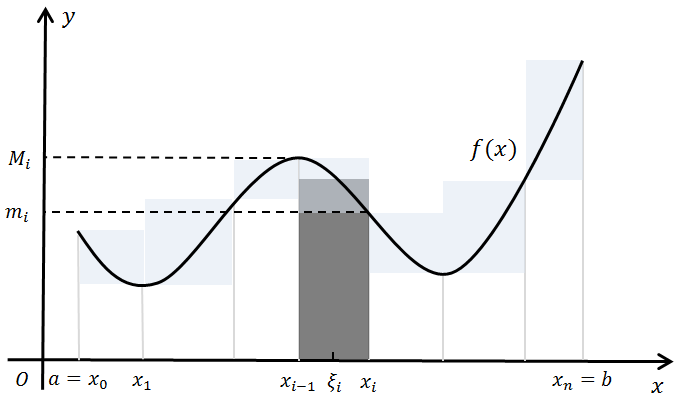
\includegraphics[width=0.7\textwidth]{image/Riemann.png}
\caption{黎曼可积的判别} \label{fig01}
\end{figure}

若条件~\eqref{eq01}~满足, 则~$f(x)$~在~$[a,\,b]$~上~的黎曼积分可表示为
\begin{equation} \label{eq02}
(R)\int_a ^b \!\! f(x) \mathrm{d}x = \lim_{\lambda \to 0} \sum^n _{i=1} f(\xi_i) \delta x_i
\end{equation}
其中, $\Delta x_i = x_i - x_{i-1}, \, \xi_i \in [x_{i-1},\,x_i]$. 注意, 这里的极限只是具有极限的形式, 不是一般意义上的极限.

由于黎曼积分对被积函数的连续性要求太强, 这样就限制了黎曼积分的应用.

例如, 狄利克雷函数
\[
D(x) = \left\{ \!\!
\begin{array}{ll}
1, & x \mbox{~为~} [0,\,1] \mbox{~上的有理数~} \\
0, & x \mbox{~为~} [0,\,1] \mbox{~上的无理数~}
\end{array}
\right.
\]
在~$[0,\,1]$~上不满足条件~\eqref{eq01}. 因此, $D(x)$~不是黎曼可积的.

\subsection*{积分与极限顺序不可交换}

设~$\{f_n(x)\}$~为~$[a,\,b]$~上的连续函数列, 且
\[
\lim_{n \to \infty} f_n(x) = f(x), \quad \forall~x \in [a,\,b]
\]
一般情况下, $f(x)$~在~$[a,\,b]$~上未必可积. 即使~$f(x)$~在~$[a,\,b]$~上可积, 也未必成立
\begin{equation} \label{eq03}
\lim_{n \to \infty} \int_a ^b \!\! f_n(x) \mathrm{d}x = \int_a ^b \!\! f(x) \mathrm{d}x
\end{equation}
为使~$f(x)$~在~$[a,\,b]$~上可积并且式~\eqref{eq03}~成立, 充分条件是~$\{f_n(x)\}$~在~$[a,\,b]$~上
一致收敛于~$f(x)$. 这不是必要条件（太强且不易验证）.

例如, 考虑~$[0,\,1]$~上的连续函数列~$f_n(x) = x^n, \, n = 1,\,2,\,\cdots$, 其极限为
\[
f(x) = \left\{ \!\!
\begin{array}{ll}
0, & x \in [0,\,1) \\
1, & x = 1
\end{array}
\right.
\]
易知, 式~\eqref{eq03}~成立, 但~$\{f_n(x)\}$~在~$[0,\,1]$~上不一致收敛于~$f(x)$
（因为连续函数列的一致收敛极限必连续, 而~$f(x)$~不连续）.

\subsection*{黎曼可积函数空间的不完备性}

$[a,\,b]$~上黎曼可积函数的全体构成的空间~$R[a,\,b]$~中, 并非每个柯西列都收敛, 即是不完备的.
而完备性在泛函分析理论中是非常重要的, 所以, $R[a,\,b]$~不是作为研究对象的理想空间.

以上几点表明, 黎曼积分有不少缺陷, 这就限制了黎曼积分的应用, 因此有必要加以改进.
20~世纪初, 法国数学家勒贝格~(1875\raisebox{0.5mm}{--}1941)~创建了一种新的勒贝格积分理论.
勒贝格积分理论是黎曼积分理论的推广和发展, 并且克服了黎曼积分理论的上述缺陷.

\section{勒贝格积分的大体思路}

为了使得很多连续性不好的函数也可积, 勒贝格提出了一种新的积分思想. 主要想法就是不从分割区间~$[a, \, b]$~着手,  而是从分割函数的值域出发.

为简单记, 这里只考虑~$f(x) \geqslant 0$~的情况. 注意到勒贝格积分的几何意义就是曲线~$y = f (x)$~的下方图形
~$G(f) = \big\{(x,\, y): \: a \leqslant x \leqslant b, \, 0 \leqslant y \leqslant f (x) \big\}$~的面积. 因此可以用下面的方式计算~$G(f)$~的面积.

令
\[
m = \inf \big\{f(x): \: x \in [a,\,b]\big\}, \quad M = \sup \big\{f(x): \: x \in [a,\,b]\big\}
\]
对~$[m,\,M]$~做分割
\[
m = y_0 < y_1 < \cdots < y_n = M
\]
记~$\lambda = \max \limits_{1 \leqslant i \leqslant n} |y_i - y_{i-1}|$. 令
\[
E_i = \big\{ x \in [a,\,b]: \: y_{i-1} \leqslant f(x) < y_i \big\}, \quad i = 1,\,2,\,\cdots,\,n
\]
则~$E_i$~是~$[a,\,b]$~的子集, 用~$|E_i|$~表示~$E_i$~的``长度''. 取~$\xi_i \in [y_{i-1},\,y_i]$, 则和式
\[
\sum^n _{i=1} \xi_i |E_i|
\]
是~$G(f)$~的近似值（图~\ref{fig02}）. 于是定义~$f(x)$~在~$[a,\,b]$~上的勒贝格积分为（若下面极限存在）
\begin{equation} \label{eq04}
(L)\int_a ^b \!\! f(x) \mathrm{d}x = \lim_{\lambda \to 0} \sum^n _{i=1} \xi_i |E_i|
\end{equation}

\begin{figure}[htbp]
\centering
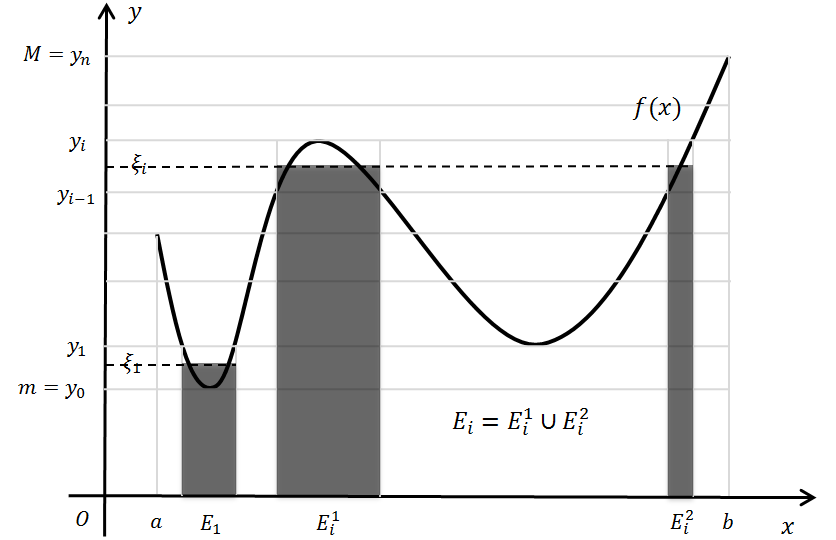
\includegraphics[width=0.8\textwidth]{image/Lebesgue.png}
\caption{勒贝格积分思想} \label{fig02}
\end{figure}

\begin{quote}
{\normalsize 对上述积分思想, 勒贝格自己曾作过一个比喻, 他说:
\begin{itemize}
  \item 假如我欠人家一笔钱, 现在要还, 此时按钞票的面值的大小分类, 然后计算每一类的面额总值, 再相加,
      这就是勒贝格积分思想;
  \item 如不按面额大小分类, 而是按从钱袋取出的先后次序来计算总数, 那就是黎曼积分思想.
\end{itemize}}
\end{quote}

按照勒贝格的方式定义积分的好处在于: 由于在每个~$E_i$~上, $f(x)$~的振幅都小于~$\lambda$,
因此很多连续性不好的函数也可积了. 但这产生了另一个困难: 要给出~$|E_i|$~的意义以及如何计算.

$|E_i|$~应该是一种类似区间长度的东西. 但是一般情况下, $E_i$~不是区间, 甚至也不是有限个不相
交区间的并, 因此必须对直线上比区间更一般的集合给出一种类似于区间长度的度量. 为
此, 勒贝格建立了测度理论, 并且在测度理论的基础上建立了勒贝格积分理论. 勒贝格 积分理论为建立近代分析理论打下了坚实的基础. 

\medskip

\section{本书的基本内容}

\qquad 本书的主要内容是紧紧围绕勒贝格积分理论的建立而展开的, 因此本书花了很大篇幅来介绍勒贝格测度理论.
由于测度理论要经常地遇到集合的运算和~$\mathbb{R}^n$~中的各种点集,  因此本书第一章先介绍了集合论和~$\mathbb{R}^n$~上点集的知识, 然后再介绍第二章勒贝格测度理论.

由于勒贝格测度理论并不能给直线上的每个集合定义测度, 只能对一部分集合即所谓``可测集''给出测度, 因此要定义~$f(x)$~的勒贝格积分, 必须要求由~$f(x)$~产生的形如
\[
E_i = \big\{ x: \: y_{i-1} \leqslant f(x) < y_i \big\}
\]
的集合是可测集, 这样的函数称为可测函数.

只有对可测函数才能定义新的积分, 因此在定义勒贝格积分之前, 需要定义可测函数并讨论可测
函数的性质, 这就是本书的第三章. 作了这些准备后, 就可以定义勒贝格积分,
并讨论勒贝格积分的性质以及与黎曼积分的关系, 构成本书的第四章.

进一步, 本书第五章利用勒贝格积分理论, 将黎曼积分的微积分学基本结果推广到更一般的函数类,
得到了勒贝格积分的微积分学基本定理、牛顿\raisebox{0.5mm}{--}莱布尼茨公式等, 使得勒贝格积分理论更加完善.

最后, 为了弥补黎曼可积函数空间不完备性缺陷, 本书在第六章介绍了所有~$p$~次幂~L-可积函数的全体构成
的空间\raisebox{0.5mm}{-----}$L^p$~空间理论, 讨论了勒贝格可积函数类的整体结构及其相互关系. $L^p$~空间的完备性和可分性为
人们解决一些具体数学问题带来了极大的便利, 为我们在其上建立分析学奠定了基础.
$L^p$~空间本身就是泛函分析课程中
巴拿赫空间的一类重要例子, 其理论也广泛地应用于微分方程、积分方程、傅里叶分析、有限元分析等许多领域.


\chapter{集合与点集} % 第一章

集合论自~19~世纪~80~年代由德国数学家康托尔创立以来, 已发展成为一个独立的数学分支, 其基本概念与方法已渗入到~20~世纪的各个数学领域. 集合与集合的运算是测度与勒贝格积分理论的基础. 本章先介绍集合论的一些基本内容, 包括集与集的运算、可列集和基数、$\R^n$~中开集、闭集及其性质、一维开集的构造、康托尔集.

\section{集合及其运算}

本节将引入集合的概念与集合的运算; 德·摩根公式是今后常用的公式; 证明两个集合相等是
经常要遇到的论证; 集列的极限是一种新型的极限, 利用上限集或下限集可以描述一些特殊的点集.

\subsection{集合的基本概念}

\begin{definition}
具有确定内容或满足一定条件的事物的全体称为集合\index{集合}(或集),
通常用大写字母如~$A,\,B, \,C$~等表示.
构成一个集合的那些事物称为集合的元素\index{元素}(或元),
通常用小写字母如~$a,\,b,\,c$~等表示.
\end{definition}

若~$a$~是集合~$A$~的元素, 则称~$a$~属于~$A$, 记为~$a \in A$; 若~$a$~不是集合~$A$~的元素, 则称~$a$~不属于~$A$, 记为~$a \notin A$. 对于给定的集合, 任一元素要么属于它, 要么不属于它, 二者必居其一\footnote{这里是指经典集合理论，模糊集合理论一个元素可以部分地隶属于某集合.}.

不含任何元素的集合称为空集, 用~$\emptyset$~表示;\  只含有限个元素的集合称为有限集;
不是有限集的集合称为无限集.

我们用~$\Z,\, \N,\, \Q,\, \R$~分别表示整数集、自然数集、有理数集和实数集.

\subsubsection*{集合的表示方法}

(1) 列举法~\raisebox{0.5mm}{-----} 列出给定集合的全部元素. 例如
\[
A = \{a,\,b,\,c\}, \; B = \{1,\,3,\,\cdots,2n-1\}
\]

(2) 描述法~\raisebox{0.5mm}{-----} $A = \{x: \: x \mbox{~具有性质~} P \}$. 例如
\[
\mathrm{ker} f = \big\{ x: \: f(x) = 0 \big\}
\]

\subsubsection*{ 集合的相等与包含}

若集合~$A$~和~$B$~具有完全相同的元素, 则称~$A$~与~$B$~相等, 记为~$A = B$.

若~$A$~中的每个元素都是~$B$~的元素, 则称~$A$~为~$B$~的子集, 记为~$A \subset B$~或~$B \supset A$.

若~$A \subset B$~且~$A \neq B$, 则称~$A$~为~$B$~的真子集, 记为~$A \subsetneqq B$.

\begin{remark}
$A = B \Longleftrightarrow A \subset B$~且~$B \subset A$. (经常用于证明两个集合相等)
\end{remark}

集合~$A$~的所有子集的全体, 称为~$A$~的幂集\index{幂集}, 记为~$2^A$.

\subsection{集合的运算}

\subsubsection*{交与并}

设~$A,\,B$~为两个集合, 由属于~$A$~或属于~$B$~的所有元素构成的集合, 称为~$A$~与~$B$~的并,
记为~$A \cup B$, 即
\[
A \cup B = \{x: \: x \in A \mbox{~或~} x \in B\}
\]

由既属于~$A$~又属于~$B$~的元素构成的集合, 称为~$A$~与~$B$~的交, 记为~$A \cap B$, 即
\[
A \cap B = \{x: \: x \in A \mbox{~且~} x \in B\}
\]
若~$A \cap B = \emptyset$, 则称~$A$~与~$B$~互不相交.

\subsubsection*{集族}

$\{A_\alpha\}_{\alpha \in \mathnormal{\Gamma}}$~称为集族\index{集族}, 其中~$\mathnormal{\Gamma}$~为指标集(有限或无限), $\alpha$~为指标.
特别地, 当~$\mathnormal{\Gamma} = \N$~时, 集族称为集列\index{集列}, 记为~$\{A_n\}^\infty_{n=1}$~或~$\{A_n\}$.

集族的并：
\[
\medcup_{\small \alpha \in \mathnormal{\Gamma}} A_\alpha = \big\{x: \: \exists~ \alpha_0 \in \mathnormal{\Gamma} \mbox{~使得~} x \in A_{\alpha_0} \big\}
\]

集族的交：
\[
\medcap_{\small \alpha \in \mathnormal{\Gamma}} A_\alpha = \big\{x: \: x \in A_\alpha, \, \forall~ \alpha \in \mathnormal{\Gamma} \big\}
\]


\subsubsection*{差与余}

由属于~$A$~但不属于~$B$~的元素构成的集合, 称为~$A$~与~$B$~的差, 记为~$A - B$~或~$A \setminus B$, 即
\[
A - B = \{x: \: x \in A \mbox{~且~} x \notin B\}
\]

通常所讨论的集合都是某一固定集~$X$~的子集, $X$~称为全集或基本集. 全集~$X$~与
子集~$A$~的差集~$X - A$, 称为~$A$~的余集, 记为~$A^c$, 即
\[
A^c = \{x: \: x \notin A\}
\]

\begin{remark}
补集是相对概念，若~$A \subset B$, 则~$B-A$~称为~$A$~关于~$B$~的补集。特别地，余集是集合关于全集的补集。
\end{remark}

\subsubsection*{笛卡儿积}

\[
A \times B = \big\{ (x,\,y): \: x \in A, \, y \in B \big\}
\]
\[
A_1 \times \cdots \times A_n = \big\{ (x_1,\, \cdots, \, x_n): \: x_i \in A_i, \, i = 1,\,\cdots,\,n \big\}
\]
例如, $n$~维欧氏空间~$\R^n = \overbrace{\R \times \cdots \times \R}^{\tiny n \mbox{~个}}$.

\subsubsection*{集合的运算及性质}

\begin{publist}
  \item[(1)] $A \cup A = A, \; A \cap A = A$;
  \item[(2)] $A \cup \emptyset = A, \; A \cap \emptyset = \emptyset$;
  \item[(3)] $A \cup B = B \cup A, \; A \cap B = B \cap A$;
  \item[(4)] $(A \cup B) \cup C = A \cup (B \cup C),  \;  (A \cap B) \cap C = A \cap (B \cap C)$;
  \item[(5)] $A \cap (B \cup C) = (A \cap B) \cup (A \cap C), \; A \cup (B \cap C) = (A \cup B) \cap (A \cup C)$, \\[0.08cm]
      $A \cap \big( \smallcup\limits_{\small \alpha \in \mathnormal{\Gamma}} B_\alpha \big) = \smallcup\limits_{\small \alpha \in \mathnormal{\Gamma}} (A \cap B_\alpha),\; A \cup \big( \smallcap\limits_{\small \alpha \in \mathnormal{\Gamma}} B_\alpha \big) = \smallcap\limits_{\small \alpha \in \mathnormal{\Gamma}} (A \cup B_\alpha)$;
      \smallskip
  \item[(6)] $A \cup A^c = X, \; A \cap A^c = \emptyset$;
  \item[(7)] $X^c = \emptyset, \; \emptyset^c = X$;
  \item[(8)] $A - B = A \cap B^c$.
\end{publist}

\begin{theorem}[德·摩根公式\index{德·摩根公式}]
设~$\{A_\alpha\}_{\alpha \in \mathnormal{\Gamma}}$~为一集族, 则

(i) $\big( \smallcup\limits_{\small \alpha \in \mathnormal{\Gamma}} A_\alpha \big)^c = \smallcap\limits_{\small \alpha \in \mathnormal{\Gamma}} A^c _\alpha$;

(ii) $\big( \smallcap\limits_{\small \alpha \in \mathnormal{\Gamma}} A_\alpha \big)^c = \smallcup\limits_{\small \alpha \in \mathnormal{\Gamma}} A^c _\alpha$.
\end{theorem}

\begin{proof}
(i) 设~$x \in \big( \smallcup\limits_{\small \alpha \in \mathnormal{\Gamma}} A_\alpha \big)^c$, 则~$x \notin \smallcup\limits_{\small \alpha \in \mathnormal{\Gamma}} A_\alpha$, 故对~$\forall~\alpha \in \mathnormal{\Gamma}, \, x \notin A_\alpha$, 即~$\forall~\alpha \in \mathnormal{\Gamma}, \, x \in A^c _\alpha$. 从而~$x \in \smallcap\limits_{\small \alpha \in \mathnormal{\Gamma}} A^c _\alpha$, 因此, $\big( \smallcup\limits_{\small \alpha \in \mathnormal{\Gamma}} A_\alpha \big)^c \subset \smallcap\limits_{\small \alpha \in \mathnormal{\Gamma}} A^c _\alpha$. 上述推理反过来也成立, 故~$\smallcap\limits_{\small \alpha \in \mathnormal{\Gamma}} A^c _\alpha \subset \big( \smallcup\limits_{\small \alpha \in \mathnormal{\Gamma}} A_\alpha \big)^c$. 因此, $\big( \smallcup\limits_{\small \alpha \in \mathnormal{\Gamma}} A_\alpha \big)^c = \smallcap\limits_{\small \alpha \in \mathnormal{\Gamma}} A^c _\alpha$. (ii)~类似可证.
\end{proof}

\subsection{上限集与下限集}

设~$\{A_n\}$~为单调集列, 若~$\{A_n\}$~单调递增, 即
\[
A_1 \subset A_2 \subset \cdots \subset A_n \subset \cdots
\]
则~$\{A_n\}$~收敛, 且~$\lim \limits_{n \to \infty} A_n = \smallcup^\infty \limits_{n=1} A_n$. 若~$\{A_n\}$~单调递减, 即
\[
A_1 \supset A_2 \supset \cdots \supset A_n \supset \cdots
\]
则~$\{A_n\}$~收敛, 且~$\lim \limits_{n \to \infty} A_n = \smallcap^\infty \limits_{n=1} A_n$.

\begin{definition}
对于一般的集列~$\{A_n\}$
\[
\medcup^\infty _{k=1} A_k \supset \medcup^\infty _{k=2} A_k \supset \cdots \supset \medcup^\infty _{k=n} A_k \supset \cdots
\]
记~$C_n = \smallcup^\infty \limits_{k=n} A_k$, 则~$\{C_n\}$~单调递减, 故~$\{C_n\}$~收敛且
\[
\lim_{n \to \infty} C_n = \medcap^\infty _{n=1} C_n = \medcap^\infty _{n=1} \medcup^\infty _{k=n} A_k
\]
称~$\smallcap^\infty \limits_{n=1} \smallcup^\infty \limits_{k=n} A_k$~为~$\{A_n\}$~的上限集\index{上限集}, 记为~$\limsup \limits_{n \to \infty} A_n$~或~$\varlimsup \limits_{n \to \infty} A_n$. 又
\[
\medcap^\infty _{k=1} A_k \subset \medcap^\infty _{k=2} A_k \subset \cdots \subset \medcap^\infty _{k=n} A_k \subset \cdots
\]
记~$D_n = \smallcap^\infty \limits_{k=n} A_k$, 则~$\{D_n\}$~单调递增, 故~$\{D_n\}$~收敛且
\[
\lim_{n \to \infty} D_n = \medcup^\infty \limits_{n=1} D_n = \medcup^\infty _{n=1} \medcap^\infty _{k=n} A_k
\]
称~$\smallcup^\infty \limits_{n=1} \smallcap^\infty \limits_{k=n} A_k$~为~$\{A_n\}$~的下限集\index{下限集}, 记为~$\liminf \limits_{n \to \infty} A_n$~或~$\varliminf \limits_{n \to \infty} A_n$. 显然有如下关系
\[
\medcap^\infty _{n=1} A_n \subset \liminf \limits_{n \to \infty} A_n \subset \limsup \limits_{n \to \infty} A_n \subset \medcup^\infty _{n=1} A_n
\]
若~$\liminf \limits_{n \to \infty} A_n = \limsup \limits_{n \to \infty} A_n$, 则称~$\{A_n\}$~收敛, 其极限记为~$\lim \limits_{n \to \infty} A_n$.
\end{definition}

\begin{proposition} \label{prop11}
设~$\{A_n\}$~为一集列, 则
\begin{eqnarray*}
\limsup_{n \to \infty} A_n = \medcap^\infty \limits_{n=1} \medcup^\infty \limits_{k=n} A_k &=& \big\{x: \: x \mbox{~属于无穷多个~} A_n \big\} \\
&=& \big\{x: \: \mbox{对~} \forall~ k \in \N, \, \mbox{都存在~} n_k \mbox{~使得~} x \in A_{n_k} \big\}
\end{eqnarray*}
\begin{eqnarray*}
\liminf_{n \to \infty} A_n = \medcup^\infty \limits_{n=1} \medcap^\infty \limits_{k=n} A_k &=& \big\{x: \: \mbox{除有限个~} A_n \mbox{~外, 都含有~} x \big\} \\
&=& \big\{ x: \: \exists~ n_0 \in \N, \, \mbox{使得~} x \in A_n, \, \forall~ n \geqslant n_0 \big\}
\end{eqnarray*}
\end{proposition}

\begin{proof}
(1) 设~$x \in \smallcap^\infty \limits_{n=1} \smallcup^\infty \limits_{k=n} A_k$, 则对~$n = 1$, 有~$x \in \smallcup^\infty \limits_{k=1} A_k$, 故~$\exists~ n_1 \in \N$, 使得~$x \in A_{n_1}$; 对~$n = n_1 + 1$, 有~$x \in \!\!\! \smallcup^\infty \limits_{k=n_1 + 1} \!\!\! A_k$, 故~$\exists~ n_2 > n_1$, 使得~$x \in A_{n_2}$; 以此类推, 得到一列~$\{n_k\}$~满足~$n_1 < n_2 < \cdots$, 且~$x \in A_{n_k}, \, \forall~k$. 因此, $x$~属于无穷多个~$A_n$.

反之, 若~$x$~属于无穷多个~$A_n$, 不妨设~$x \in A_{n_k}, \, k =1,\,2,\,\cdots$, 且~$n_1 < n_2 < \cdots$,
则对~$\forall~n \in \N$, 都存在~$n_k > n$. 从而~$x \in A_{n_k} \subset \smallcup^\infty \limits_{k = n} A_k$. 因此, $x \in \smallcap^\infty \limits_{n=1} \smallcup^\infty \limits_{k=n} A_k$.

(2) $x \in \smallcup^\infty \limits_{n=1} \smallcap^\infty \limits_{k=n} A_k$ $\Longleftrightarrow$ $\exists~n_0 \in \N$, 使得~$x \in \smallcap^\infty \limits_{k=n_0} A_k$ $\Longleftrightarrow$ $x \in A_n, \, \forall~ n \geqslant n_0$. 
\end{proof}

\medskip

\begin{example}
设~$A_{2n +1} = \big[0,\,2-1/(2n+1)\big], \, n = 0,\,1,\,2,\,\cdots, \; A_{2n} = \big[0,\,1+1/2n\big], \, n = 1,\,2,\,\cdots$, 求~$\liminf \limits_{n \to \infty} A_n$~与~$\limsup \limits_{n \to \infty} A_n$.
\end{example}

\begin{solution}
注意到
\[
[0,\,1] \subset \medcap^\infty _{n=1} A_n \subset \liminf \limits_{n \to \infty} A_n \subset \limsup \limits_{n \to \infty} A_n \subset \medcup^\infty _{n=1} A_n \subset [0,\,2)
\]
故只需考察~$(1,\,2)$~中的点. 对~$\forall~x \in (1,\,2)$, 存在~$n_0 \in \N$(与~$x$~有关), 使得
\[
1+ \frac{1}{2n} < x < 2- \frac{1}{2n+1}, \quad \forall~ n \geqslant n_0
\]
即当~$n \geqslant n_0$~时, 有~$x \notin A_{2n}, \, x \in A_{2n+1}$. 这说明: (i)~$x$~不能``除有限个~$A_n$~外, 都含有~$x$'', 即~$x \notin \liminf \limits_{n \to \infty} A_n$; (ii)~``$x$~属于无穷多个~$A_n$'', 故~$x \in \limsup \limits_{n \to \infty} A_n$. 因此, $\liminf \limits_{n \to \infty} A_n = [0,\,1]$, $\limsup \limits_{n \to \infty} A_n = [0,\,2]$.
\end{solution}

\medskip

\begin{example} \label{ex112} 设~$f_n(x),\,f(x)$~为~$\R$~上的实值函数, 则所有~$\{f_n(x)\}$~不收敛于~$f(x)$~的
点~$x$~构成的集合~$D$~可表示为
\[
D = \medcup^\infty _{k=1} \medcap^\infty _{N=1} \medcup^\infty _{n=N} \Big\{x: \: |f_n(x)-f(x)| \geqslant \frac{1}{k}\Big\}
\]
\end{example}

\begin{proof}
若~$x \in D$, 则~``$f_n(x) \nrightarrow f(x)$'', 即~$\exists~\varepsilon_0 > 0$, 对~$\forall~k \in \N, \, \exists~ n_k \geqslant k$, 使得
\[
|f_{n_k}(x)-f(x)| \geqslant \varepsilon_0
\]
记~$E_n(\varepsilon_0) = \big\{x: \: |f_n(x)-f(x)| \geqslant \varepsilon_0 \big\}$, 则由命题~\ref{prop11}~知,
\[
D = \medcap^\infty _{N=1} \medcup^\infty _{n=N} E_n(\varepsilon_0), \quad \exists~\varepsilon_0 > 0
\]

考虑到~$\varepsilon_0$~的取法, 不妨设~$\varepsilon_0 = 1/k_0, \, k_0 \in \N$. 因此
\begin{eqnarray*}
D &=& \medcup^\infty _{k=1} \medcap^\infty _{N=1} \medcup^\infty _{n=N} E_n \Big(\frac{1}{k}\Big) \\
&=& \medcup^\infty _{k=1} \medcap^\infty _{N=1} \medcup^\infty _{n=N} \Big\{x: \: |f_n(x)-f(x)| \geqslant \frac{1}{k}\Big\}
\end{eqnarray*}
\end{proof}

\begin{remark}
由于收敛点集是不收敛点集的余集, 由德·摩根公式, 所有~$\{f_n(x)\}$~收敛于~$f(x)$~的
点~$x$~构成的集合~$C$~可表示为
\[
C = \medcap^\infty _{k=1} \medcup^\infty _{N=1} \medcap^\infty _{n=N} \Big\{x: \: |f_n(x)-f(x)| < \frac{1}{k}\Big\}
\]
\end{remark}

\section{映射与集合的对等}

\subsection{映射}

数学分析中研究的函数可以看成是数集与数集之间的一种对应关系, 把数集换成一般的集合就得到映射的概念.

\begin{definition}
设~$A,\,B$~为非空集, 若存在对应法则~$f$, 使得对每个~$x \in A$~都有唯一确定的~$y \in B$~与之对应, 则称对应法则~$f$~为从~$A$~到~$B$~的映射\index{映射}.
记为~$f:\: A \rightarrow B$, 其表达形式为~$y = f(x), \, x \in A$.

$A$~称为~$f$~的定义域\footnote{函数的定义域, 通常是让函数表达式有意义的自变量的全体,
或根据实际问题的需要所确定的自变量范围. }, 记为~$D(f)$.

$A$~在~$f$~下的象称为~$f$~的值域, 记为~$R(f)$, 即
\[
R(f) = f(A)=\{f(x): \: x \in A\}
\]

集合~$B_0 \subset B$~在~$f$~下的原象, 记为~$f^{-1}(B_0)$, 即
\[
f^{-1}(B_0)=\{x \in A: \: f(x) \in B_0\}
\]
\end{definition}

除了函数之外, 我们还经常遇到许多其他的映射. 例如, 定积分可以看作是可积函数集到
实数集的映射, 求导运算可以看作是可导
函数集到函数集的映射, 线性代数中的线性变换就是线性空间到线性空间的映射等.

\begin{remark}
关于映射的定义, 我们作以下几点说明:

(1) 对每一个~$x \in A$, 只能有唯一的~$y \in B$~与它对应;

(2) $f(A) \subset B$, 不一定有~$f(A) = B$;


(3) 映射是由定义域和对应法则共同确定的, 但对应法则的表达形式可能不唯一. 例如
  \[
  y = |x|, \,\, x \in \R \quad \mbox{和} \quad y = \sqrt{x^2}, \,\, x \in \R
  \]

(4) 值域中的元可以是集合. 例如~$A = \N, \, B = \{B_n\}^\infty_{n=1}, \, \phi(n)=B_n$;

(5) 定义域中的元也可以是集合. 例如~$A$~可列, $\mathcal{D} \subset 2^A$, 定义~$\phi: \: \mathcal{D} \rightarrow \{0\} \cup \N$~为
      \[
      \phi(A_0) = A_0 \mbox{~中元素个数}, \quad  A_0 \in \mathcal{D}
      \]
\end{remark}

\begin{definition}
若~$x_1 \neq x_2$, 则~$f(x_1) \neq f(x_2)$, 则称~$f$~为单射\index{单射}

若~$f(A)=B$, 即~$\forall y \in B$, 都存在~$x \in A$~使得~$f(x) = y$, 则称~$f$~为满射\index{满射}(或到上的). 

既单且满的映射, 称为一一映射\index{一一映射}(或双射).
\end{definition}

\begin{figure}[htbp]
\centering
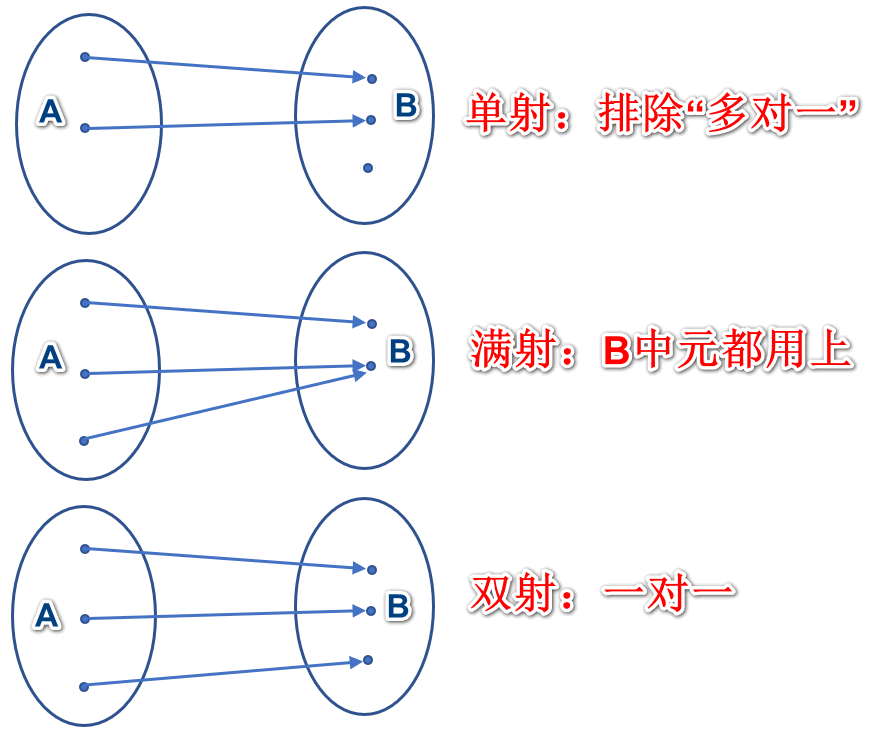
\includegraphics[width=0.5\textwidth]{image/mapping.png}
\caption{单射/满射/双射示意图} \label{fig:mapping}
\end{figure}

\begin{definition}
设~$f: \: A \rightarrow B$~为一一映射, 则对每个~$y \in B$, 都有唯一确定的~$x \in A$~满足~$y = f(x)$. 定义~$f^{-1}: \: B \rightarrow A$~为~$f^{-1}(y) = x$, 则称~$f^{-1}$~为~$f$~的逆映射.
\end{definition}

逆映射是反函数概念的推广, 由逆映射的定义
\[
f^{-1}\big(f(x)\big) = x, \quad x \in A
\]
\[
f\big(f^{-1}(y)\big) = y, \quad y \in B
\]

\begin{definition}
设映射~$f: \: A \rightarrow B, \, g: \: B \rightarrow C$, 定义~$g \circ f: \: A \rightarrow C$~为
\[
g \circ f(x) = g \big(f(x)\big), \quad x \in A
\]
称为~$f$~与~$g$~的复合映射.

设映射~$f: \: A \rightarrow B$, $A_0 \subset A$, 若~$g: \: A_0 \rightarrow B$~满足
\[
g(x) = f(x), \quad x \in A_0
\]
则称~$g$~为~$f$~在~$A_0$~上的限制, 记为~$g = f|_{A_0}$, 也称$f$~为~$g$~在~$A$~上的延拓.
\end{definition}

集合的特征函数是本书常用到的一种特殊映射. 

\begin{definition}
集合~$E$~的特征函数\index{特征函数}定义为
\[
\chi_E(x) = \left\{\!\!
\begin{array}{ll}
1, & x \in E \\
0, & x \notin E
\end{array}
\right.
\]
\end{definition}

特征函数~$\chi_E$~在一定意义上反映出集合~$E$~本身的特征, 可以通过它来表示各种集合关系. 例如, $A = B$~$\Leftrightarrow$~$\chi_A(x) = \chi_B(x)$; $A \subset B$~$\Leftrightarrow$~$\chi_A(x) \leqslant \chi_B(x)$. 容易验证:

(i) $\chi_{A \cap B}(x) = \chi_A(x) \cdot \chi_B(x)$;

(ii) $\chi_{A \cup B}(x) = \chi_A(x) + \chi_B(x) - \chi_A(x) \cdot \chi_B(x)$;

(iii) $\chi_{A - B}(x) = \chi_A(x) [1 - \chi_B(x)]$.

\begin{proposition}
对于映射, 下列事实成立:

(i) 若~$A \subset B$, 则~$f(A) \subset f(B)$;

(ii) $f\big(\smallcup\limits_{\alpha \in I} {A_\alpha} \big) = \smallcup\limits_{\alpha \in I} {f(A_\alpha)}$;

(iii) $f\big(\smallcap\limits_{\alpha \in I} {A_\alpha} \big) \subset \smallcap\limits_{\alpha \in I} {f(A_\alpha)}$, 当且仅当~$f$~为单射时, ``$=$''成立;

(iv) $f\big(f^{-1}(B)\big) \subset B$, 当且仅当~$f$~为满射时, ``$=$''成立;

 ~~~~~ $A \subset f^{-1}\big(f(A)\big)$, 当且仅当~$f$~为单射时, ``$=$''成立;

(v) $f^{-1}(B^c) = \big(f^{-1}(B)\big)^c$.
\end{proposition}

\begin{proof}
(i)~显然, (ii)~和~(v)~容易验证.

(iii) 只证明两个集合的情形. 注意到~$A_1 \cap A_2 \subset A_1, \, A_1 \cap A_2 \subset A_2$, 由~(i)~知
\[
f(A_1 \cap A_2) \subset f(A_1), \quad f(A_1 \cap A_2) \subset f(A_2)
\]
故~$f(A_1 \cap A_2) \subset f(A_1) \cap f(A_2)$.

设~$y \in f(A_1) \cap f(A_2)$, 则~$y \in f(A_1)$~且~$y \in f(A_2)$, 故存在~$x_1 \in A_1,\, x_2 \in A_2$~使得~$y = f(x_1) = f(x_2)$. 由于~$f$~是单射, 则必有~$x_1 = x_2 = x$. 所以
\[
x \in A_1 \cap A_2, \quad y = f(x) \in f(A_1 \cap A_2)
\]
故
\[
f(A_1) \cap f(A_2) \subset f(A_1 \cap A_2)
\]
因此, ``$=$''成立.

反之, 假设~$f$~不是单射, 则存在~$x_1 \neq x_2$~使得~$f(x_1) = f(x_2)$. 构造集合~$A_1 = \{x_1\}, \, A_2 = \{x_2\}$, 则~$A_1 \cap A_2 = \emptyset$, 从而~$f(A_1 \cap A_2) = \emptyset$. 而
\[
f(A_1) \cap f(A_2) = \{f(x_1)\} \neq \emptyset
\]
故~$f(A_1 \cap A_2) \neq f(A_1) \cap f(A_2)$. 矛盾.

(iv) (1) 设~$y \in f\big(f^{-1}(B)\big)$, 则存在~$x \in f^{-1}(B)$~使得~$y = f(x)$. 故~$y = f(x) \in B$. 因此, $f\big(f^{-1}(B)\big) \subset B$.

设~$y \in B$, $f$~为满射, 则存在~$x \in A$~使得~$y = f(x)$. 故~$x \in f^{-1}(y) \subset f^{-1}(B)$, 从而~$y = f(x) \in f\big(f^{-1}(B)\big)$, 于是~$B \subset f\big(f^{-1}(B)\big)$, 因此, ``$=$''成立.

反之, 假设~$f$~不是满射, 则~$f(A) \subsetneqq B$. 由于~$f^{-1}(B) \subset A$, 故
\[
f\big(f^{-1}(B)\big) \subset f(A) \subsetneqq B
\]
与~$B = f\big(f^{-1}(B)\big)$~矛盾.

(2) 设~$x \in A$, 则~$f(x) \in f(A)$, 故~$x \in f^{-1}\big(f(A)\big)$. 因此, $A \subset f^{-1}\big(f(A)\big)$.

设~$x \in f^{-1}\big(f(A)\big)$, 则~$f(x) \in f(A)$. 再由~$f$~是单射, 则必有~$x \in A$. 从而~$f^{-1}\big(f(A)\big) \subset A$. 因此, ``$=$''成立.

反之, 假设~$f$~不是单射, 则存在~$x_1 \neq x_2$~使得~$f(x_1) = f(x_2)$. 构造集合~$A = \{x_1\}$, 则~$f(A) = \{f(x_1)\}$. 故~$\{x_1, \, x_2\} \subset f^{-1}\big(f(A)\big)$, 从而~$A \neq f^{-1}\big(f(A)\big)$. 矛盾.
\end{proof}

\subsection{集合的对等}

研究集合的一个基本问题, 就是比较两个集合包含元素的多与少. 对于有限集, 我们可以通过分别数数的方法来比较. 例如, 比较某班学生人数与某教室座位数的多少, 就可以分别数出学生人数和座位个数, 然后比较两个数的大小来确定. 那么, 两个无限集是否可以比较元素的多少呢？

初看起来, 无限集都含有无限多个元素, 似乎不能比较元素的多与少, 现在我们换一种方式来考虑这个问题. 在比较两个有限集元素多少的时候, 还可以采用另一种方法, 即``一一对应''的方法. 比如前面的例子中, 可以考虑让一个学生坐一个座位(建立一一对应关系), 若学生和座位都恰好没有剩余, 则学生与座位数相等; 若仍有站着的学生, 则说明学生人数多; 若仍有空座位, 则说明座位数多.

用集合语言来描述就是, 若集~$A$~与~$B$~之间能建立一种一一对应, 则~$A$~与~$B$~具有同样多的元素. 如果~$A$~与~$B$~的一个真子集之间能建立一一对应, 则~$A$~的元素比~$B$~的元素少. 这种方法也适用于无限集的情形.

因此, 可以利用映射来研究比较两个集合元素多少的问题.

\begin{definition}
设~$A, \, B$~为非空集, 若存在从~$A$~到~$B$~的一一映射, 则称~$A$~与~$B$~对等\index{对等},
记为~$A \sim B$. 规定~$\emptyset \sim \emptyset$.
\end{definition}

$A$~与~$B$~对等就是两个集合的元素可以建立一一对应的关系. 对等关系具有如下性质:

(i) (反身性)$A \sim A$;

(ii) (对称性)若~$A \sim B$, 则~$B \sim A$;

(iii) (传递性)若~$A \sim B, \, B \sim C$, 则~$A \sim C$.

\medskip

\begin{example} \label{ex1.2.1}
自然数集~$\N$~$\sim$~正偶数集~$\sim$~正奇数集~$\sim$~整数集~$\Z$.
\end{example}

\begin{proof}
正偶数集~$= \{2n: \: n \in \N\}$; \quad 正奇数集~$= \{2n-1: \: n \in \N\}$;

\qquad \quad $\Z = \{(-1)^{n+1} [n/2]: \: n \in \N\}$.
\end{proof}

\medskip

\begin{example} \label{ex1.2.2}
$(-1, \, 1)~\sim~\R$.
\end{example}

\begin{proof}
$f(x) = \tan \dfrac{\pi}{2}x$.
\end{proof}

\medskip

\begin{example} \label{ex1.2.3}
\{去掉一点的圆周\}~$\sim~\R$.
\end{example}

\begin{proof}
如图~\ref{fig1.1.1}, 设圆周为~$C$, 从除去的点~$P$~作过圆心的直线, 取与该直线垂直且与圆周相切(不过点~$P$~)的直线
表示实轴~$\R$. 对于~$C - \{P\}$~上的每一点~$c$, 从点~$P$~作过点~$c$~的直线必与实轴相交于某点,
记为~$x$. 建立一一对应: $s: \: \R \rightarrow C - \{P\}$~为~$s(x) = c$. (点~$P$~对应~$\infty$)
\end{proof}

\begin{figure}[!htb]
\centering
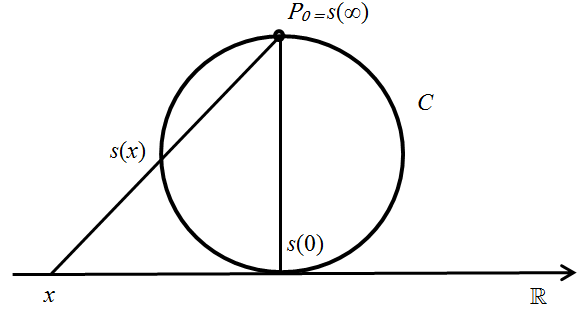
\includegraphics[width=0.56\textwidth]{image/duideng.png}
\caption{去掉一点的圆周与实轴对等} \label{fig1.1.1}
\end{figure}

类似地, 球面去掉一点与平面上的点集对等.

证明两个集合对等, 通常采用中间集合过渡(例~\ref{ex1.2.1})、寻找一一映射
(例~\ref{ex1.2.2})等方法. 另一个
重要方法就是利用伯恩斯坦定理.

\begin{lemma} \label{lem1.2.1}
设~$A,\,B$~为非空集, 若~$f: \: A \rightarrow B, \, g: \: B \rightarrow A$, 则~$A$~与~$B$~存在如下分解:

(i) $A = A_1 \cup A_2, \, B = B_1 \cup B_2$;

(ii) $A_1 \cap A_2 = \emptyset, \, B_1 \cap B_2 = \emptyset$;

(iii) $f(A_1) = B_1, \, g(B_2) = A_2$.
\end{lemma}

\begin{proof}
作集族
\[
\mathnormal{\Gamma} = \{E \subset A: \: E \cap g\big(B-f(E)\big) = \emptyset\}
\]
$\mathnormal{\Gamma}$~中的元称为~$A$~中的隔离集. 令~$A_1 = \smallcup \limits_{E \in \mathnormal{\Gamma}} E$, 则~$A_1 \in \mathnormal{\Gamma}$. 实际上, 对任意的~$E \in \mathnormal{\Gamma}$, 都有~$E \subset A_1$, 再由~$E \cap g\big(B-f(E)\big) = \emptyset$~知
\[
E \cap g\big(B-f(A_1)\big) = \emptyset
\]
从而
\[
A_1 \cap g\big(B-f(A_1)\big) = \smallcup \limits_{E \in \mathnormal{\Gamma}} \big[E \cap g\big(B-f(E)\big)\big] = \emptyset
\]
因此, $A_1$~是~$A$~中隔离集, 且是~$\mathnormal{\Gamma}$~中的最大元.

现在令~$B_1 = f(A_1), \, B_2 = B - B_1, \, A_2 = g(B_2)$, 则
\[
A_1 \cap A_2 = A_1 \cap g\big(B - f(A_1)\big) = \emptyset
\]
下面只需验证~$A_1 \cup A_2 = A$.

若不然, 则存在~$x_0 \in A, \, x_0 \notin A_1 \cup A_2$. 令~$A_0 = A_1 \cup \{x_0\}$, 由于~$B_1 = f(A_1) \subset f(A_0)$, 故
\[
B - f(A_0) \subset B - B_1 = B_2
\]
从而
\[
g\big(B - f(A_0)\big) \subset g(B_2) = A_2
\]
再由~$A_1 \cap A_2 = \emptyset$~以及~$x_0 \notin A_2$~知
\[
A_1 \cap g\big(B - f(A_0)\big) = \emptyset, \quad x_0 \notin g\big(B - f(A_0)\big)
\]
因此
\[
A_0 \cap g\big(B - f(A_0)\big) = \emptyset
\]
故~$A_0 \in \mathnormal{\Gamma}$. 这与~$A_1$~是~$\mathnormal{\Gamma}$~中的最大元矛盾.
\end{proof}

\begin{theorem}[伯恩斯坦定理\index{伯恩斯坦定理}] \label{Bernstein} 
若~$A$~与~$B$~的某子集对等, $B$~与~$A$~的某子集对等, 则~$A \sim B$.
\end{theorem}

\begin{proof}
由题设存在单射~$f: \: A \rightarrow B, \, g: \: B \rightarrow A$, 利用引理~\ref{lem1.2.1}~可得到~$A$~与~$B$~的分解
\[
A = A_1 \cup A_2, \quad B = B_1 \cup B_2
\]
\[
f(A_1) = B_1, \quad g(B_2) = A_2
\]
其中, $A_1 \cap A_2 = \emptyset, \, B_1 \cap B_2 = \emptyset$. 注意到~$f: \: A_1 \rightarrow B_1, \, g^{-1}: \: A_2 \rightarrow B_2$~是一一映射, 作映射
\[
F(x) = \left\{\!\!
\begin{array}{ll}
f(x), & x \in A_1 \\
g^{-1}(x), & x \in A_2
\end{array}
\right.
\]
则~$F: \: A \rightarrow B$~是一一映射, 从而~$A \sim B$.
\end{proof}

\medskip

\begin{example} \label{ex1.2.4}
$[-1,\,1] \sim \R$.
\end{example}

\begin{proof}
由例~\ref{ex1.2.2}, $\R \sim (-1,\,1) \subset [-1,\,1]$; 又~$[-1,\,1] \sim [-1,\,1] \subset \R$. 由伯恩斯坦定理, $[-1,\,1] \sim \R$.
\end{proof}

\subsection{集合的基数}

\begin{definition}
设~$A, \, B$~为两个集合, 若~$A \sim B$, 则称~$A$~与~$B$~的基数\index{基数}或势相同, 记为~$\overline{\overline A} = \overline{\overline B}$.
\end{definition}

由对等的传递性, 所有互相对等的集合都有相同的基数, 可见基数反映了对等集在元素数量级别上
的共性. 若~$A$~与
~$B$~的一个子集对等, 则~$\overline{\overline A} \leqslant \overline{\overline B}$. 结合映射的定义,  映射与基数之间存在如下关系:

(i) 若存在从~$A$~到~$B$~的单射, 则~$\overline{\overline A} \leqslant \overline{\overline B}$;

(ii) 若存在从~$A$~到~$B$~的满射, 则~$\overline{\overline A} \geqslant \overline{\overline B}$;

(iii) 若存在从~$A$~到~$B$~的一一映射, 则~$\overline{\overline A} = \overline{\overline B}$. \\
\noindent 因此, 伯恩斯坦定理也可以改写为下面的形式:

\begin{theorem}
若集合~$A,\,B$~满足~$\overline{\overline A} \leqslant \overline{\overline B}, \, \overline{\overline B} \leqslant \overline{\overline A}$, 则~$\overline{\overline A} = \overline{\overline B}$.
\end{theorem}

规定~$\overline{\overline{\emptyset}} = 0$. 若存在自然数~$n$, 使得~$A \sim \{1,\,2,\,\cdots, \, n\}$, 则称~$A$~为有限集, 并记~$\overline{\overline A} = n$. 因此有限集的基数等于该集合元素的个数. 这样,  集合的基数就是有限集元素个数的推广.

不是有限集的集合称为无限集. 有限集和无限集的本质区别在于: 有限集不能与其真子集对等,
而无限集必与其某个真子集对等.

\begin{theorem} \label{thm1.2.2}
有限集不可能与其某个真子集对等.
\end{theorem}

\begin{proof}
用数学归纳法证明, $n = 1$, 显然. 假设~$n = k$~时, 结论成立.

当~$n = k + 1$~时, 若存在~$A$~的某个真子集~$A_0$~使得~$A \sim A_0$, 则存在一一映射~$\varphi: \: A \rightarrow A_0$. 下面分两种情况:

(1) $\exists \, \ a \in A$, 使得~$\varphi(a) = a$.

令~$A_1 = A - \{a\}, \, A_2 = A_0 - \{a\}$, 则~$A_2$~是~$A_1$~的真子集, $\overline{\overline {A_1}} = k$. 而~$\varphi|_{A_1}$~是~$A_1$~到~$A_2$~的一一映射, 故~$A_1 \sim A_2$. 这与假设矛盾.

(2) $\forall \, a \in A$, 都有~$\varphi(a) \neq a$.

$A_0$~是~$A$~的真子集, 则存在~$x_0 \in A, \, x_0 \notin A_0$. 令
\[
A_3 = A - \{x_0\}, \quad A_4 = A_0 - \{\varphi(x_0)\}
\]
注意到~$x_0 \notin A_0$~以及~$A_0$~是~$A$~的真子集, 则~$A_4$~是~$A_3$~的子集. 又由于
\[
\varphi(x_0) \in A_0 \subset A, \quad \varphi(x_0) \neq x_0
\]
故~$\varphi(x_0) \in A - \{x_0\} = A_3$, 而~$\varphi(x_0) \notin A_0 - \{\varphi(x_0)\} = A_4$. 从而~$A_4$~是~$A_3$~的真子集,  于是~$\overline{\overline {A_3}} = k$, ~$\varphi|_{A_3}$~是~$A_3$~到~$A_4$~的一一映射, 故~$A_3 \sim A_4$. 这与假设矛盾.
\end{proof}

\section{可列集}

\subsection{可列集的定义}

无限集中最简单、最常见、包含元素个数最少的一类就是可列集.

\begin{definition}
与自然数集~$\N$~对等的集合称为可列集\index{可列集},
其基数记为~$\aleph_0$(读作阿列夫零). 有限集和可列集统称
为可数集\index{可数集}.
\end{definition}

\begin{remark}
$A$~是可列集, 当且仅当~$A$~可以写成~$A = \{a_n\}_{n = 1} ^\infty$.
\end{remark}

\begin{proof}
$A$~可列, 则存在~$\N$~到~$A$~的一一映射~$\varphi$, 记为~$\varphi(n) = a_n, \, n \in \N$, 则~$A = \{a_n\}_{n = 1} ^\infty$. 反过来, 若~$A = \{a_n\}_{n = 1} ^\infty$, 将每个~$a_n$~与其下标~$n$~建立一一对应, 则~$A$~与~$\N$~对等, 从而是可列集.
\end{proof}

由~\S~1.2~例~\ref{ex1.2.1}, 自然数集、正偶数集、正奇数集、整数集都是可列集.

\subsection{可列集的性质}

\begin{proposition} \label{thm1.3.1}
任何无限集必包含一个可列子集.
\end{proposition}

\begin{proof}
设~$A$~为无限集. 从~$A$~中任取一元~$a_1$; 由于~$A - \{a_1\} \neq \emptyset$, 取~$a_2 \in A - \{a_1\}$; 又~$A - \{a_1, \, a_2\} \neq \emptyset$, 取~$a_3 \in A - \{a_1, \, a_2\}$; $\cdots\cdots$,  因为~$A$~是无限集, 这一过程可以一直继续下去, 从而得到~$A$~的一个可列子集~$\{a_n\}_{n = 1} ^\infty$.
\end{proof}

该定理也说明, 众多无限集中, 最小的基数是可列集的基数~$\aleph_0$.

\begin{corollary} \label{cor1.3.1}
无限集必与其某个真子集对等.
\end{corollary}

\begin{proof}
设~$A$~为无限集, 由定理~\ref{thm1.3.1}, 存在可列子集~$\{a_n\}_{n = 1} ^\infty \subset A$. 令~$B = A - \{a_1\}$, 则~$B$~是~$A$~的真子集. 定义映射
\begin{eqnarray*}
\varphi(a_k) &=& a_{k+1}, \quad k = 1, \, 2, \, \cdots \\
\varphi(x) &=& x, \quad x \in A - \{a_n\}_{n = 1} ^\infty
\end{eqnarray*}
则~$\varphi: \: A \rightarrow B$~是一一映射, 故~$A \sim B$.
\end{proof}

结合定理~\ref{thm1.2.2}~与推论~\ref{cor1.3.1}, 可以得到有限集和无限集的如下等价定义
\[
\left\{\!\!
\begin{array}{lcl}
A \mbox{~是有限集~} & \Longleftrightarrow & A \mbox{~不与其任意真子集对等~} \\
A \mbox{~是无限集~} & \Longleftrightarrow & A \mbox{~必与其某个真子集对等~}
\end{array}
\right.
\]

\begin{proposition} \label{thm1.3.2}
可列集的任何无限子集都是可列集.
\end{proposition}

\begin{proof}
设~$A = \{a_1, \, a_2, \, \cdots, \, a_n, \, \cdots\}$. $B$~是~$A$~的无限子集, 按照~$A$~中元素的次序依次寻找~$B$~中元素, 分别记为~$a_{n_1},\, a_{n_2}, \, \cdots$, 则~$B = \{a_{n_1}, \, a_{n_2}, \, \cdots, \, a_{n_k}, \, \cdots\}$~为可列集.
\end{proof}

\begin{proposition} \label{thm1.3.4}
有限集与可列集的并集是可列集.
\end{proposition}

\begin{proof}
设~$A = \{a_1, \, a_2, \, \cdots, \, a_n\}, \, B = \{b_1, \, b_2, \, \cdots\}$. 不妨设~$A \cap B = \emptyset$, 则
\[
A \cup B = \{a_1, \, a_2, \, \cdots, \, a_n, \, b_1, \, b_2, \, \cdots\}
\]
可列.
\end{proof}

\begin{proposition} \label{thm1.3.5}
有限个可列集的并集是可列集.
\end{proposition}

\begin{proof}
设~$A_k = \{a_1 ^{(k)}, \, a_2 ^{(k)}, \, a_3 ^{(k)}, \, \cdots\}, \, k = 1,\,2,\, \cdots, \,n$~为可列集, 则~$\smallcup \limits_{k=1} ^n A_k$~的元素可以按下面的方式编号排序
\[
\begin{array}{cccccc}
A_1 & = & \{~a_1 ^{(1)} & a_2 ^{(1)} & a_3 ^{(1)} & \cdots~\} \\
    &   &   \downarrow  & \downarrow & \downarrow &           \\
A_2 & = & \{~a_1 ^{(2)} & a_2 ^{(2)} & a_3 ^{(2)} & \cdots~\} \\
    &   &   \downarrow  & \downarrow & \downarrow &           \\
    &   &   \vdots      &    \vdots  &    \vdots  &           \\
    &   &   \downarrow  & \downarrow & \downarrow &           \\
A_n & = & \{~a_1 ^{(n)} & a_2 ^{(n)} & a_3 ^{(n)} & \cdots~\}
\end{array}
\]
必要时删掉后续的重复元, 可得到
\[
\medcup \limits_{k=1} ^n A_k = \big\{a_1 ^{(1)}, \, \cdots, \, a_1 ^{(n)}, \, a_2 ^{(1)}, \, \cdots, \, a_2 ^{(n)}, \, a_3 ^{(1)}, \, \cdots\big\}
\]
可列.
\end{proof}

\begin{proposition} \label{thm1.3.6}
可列个可列集的并集是可列集.
\end{proposition}

\begin{proof}
设~$\{A_n\}_{n=1} ^\infty$~为一列可列集, 则~$\smallcup \limits_{n=1} ^\infty A_n$~的元素可以按下面的方式编号排序
\[
\begin{array}{cccccccccc}
A_1 &=& \{~a_1 ^{(1)} & \rightarrow & a_2 ^{(1)} && a_3 ^{(1)} & \rightarrow & a_4 ^{(1)} & \cdots~\} \\
    &&                &  \swarrow   &      & \nearrow &        &  \swarrow   &            &   \\
A_2 &=& \{~a_1 ^{(2)} &  & a_2 ^{(2)} && a_3 ^{(2)} &  & a_4 ^{(2)} & \cdots~\} \\
    &&   \downarrow   &  \nearrow   &      & \swarrow &        &  &  &   \\
A_3 &=& \{~a_1 ^{(3)} &  & a_2 ^{(3)} && a_3 ^{(3)} &  & a_4 ^{(3)} & \cdots~\} \\
    & &     \vdots    &  &   \vdots   &&    \vdots  &  &   \vdots   &           \\
A_n &=& \{~a_1 ^{(n)} &  & a_2 ^{(n)} && a_3 ^{(n)} &  & a_4 ^{(n)} & \cdots~\} \\
    & &     \vdots    &  &    \vdots  &&    \vdots  &  &   \vdots   &
\end{array}
\]
必要时删掉后续的重复元, 可得到
\[
\medcup \limits_{n=1} ^\infty A_n = \big\{a_1 ^{(1)}, \, a_2 ^{(1)}, \, a_1 ^{(2)}, \, \cdots, \, a_1 ^{(2n+1)}, \, a_2 ^{(2n)}, \, \cdots, \, a_{2n+1} ^{(1)}, \, \cdots\big\}
\]
(依次是下标之和等于~$2, \, 3, \, \cdots, \, 2n+2, \, \cdots$)可列.
\end{proof}

\begin{proposition} \label{thm1.3.7}
若~$A$~为无限集, $B$~为有限集或可列集, 则~$\overline{\overline{A \cup B}} = \overline{\overline{A}}$.
\end{proposition}

\begin{proof}
不妨设~$A \cap B = \emptyset$, 否则用~$B - A$~代替~$B$~即可. $A$~为无限集, 由定理~\ref{thm1.3.1}, $A$~包含一个可列子集~$A_1$. 由于~$A_1 \cup B$~是可列集, 故~$A_1 \cup B \sim A_1$. 注意到~$(A - A_1) \cap (A_1 \cup B) = \emptyset$, 则有
\begin{eqnarray*}
A \cup B &=& (A - A_1) \cup A_1 \cup B \\
&=& (A - A_1) \cup (A_1 \cup B) \sim (A - A_1) \cup A_1 = A
\end{eqnarray*}
因此, $\overline{\overline{A \cup B}} = \overline{\overline{A}}$.
\end{proof}

\subsection{可列集的例}

\begin{example} \label{ex1.3.1}
有理数集~$\Q$~是可列集.
\end{example}

\begin{proof}
$\Q = \Q^+ \cup \{0\} \cup \Q^-$, 其中~$\Q^+, \, \Q^-$~分别表示正、负有理数集. 由对称性以及定理~\ref{thm1.3.4}~和
定理~\ref{thm1.3.5}, 只需证明$\Q^+$~可列.

对每个~$n \in \N$, 令
\[
A_n = \Big\{\frac{1}{n},\,\frac{2}{n},\,\frac{3}{n},\,\cdots\Big\}
\]
则~$A_n$~可列. 又~$\Q^+ = \smallcup \limits_{n=1} ^\infty A_n$(除去重复元), 由可列集性质知~$\Q^+$~可列.
\end{proof}

\medskip

\begin{example} \label{ex1.3.2}
实轴上互不相交的开区间至多有可列个.
\end{example}

\begin{proof}
开区间的长度大于~$0$, 故必含有有理数, 在每一个开区间内取出一个有理数. 因为开区间互不相交,
所以取出的有理数都不相等, 从而这些有理数构成~$\Q$~的一个子集. 又~$\Q$~是可列集,
故这样的开区间至多有可列个.
\end{proof}

\medskip

\begin{example} \label{ex1.3.3}
设~$A, \, B$~为可列集, 则~$A \times B$~是可列集.
\end{example}

\begin{proof}
注意到
\[
A \times B = \big\{(x,\,y): \: x \in A, \, y \in B\big\} = \medcup_{x \in A} \big\{(x,\,y): \: y \in B\big\}
\]
由可列集性质知~$A \times B$~可列.
\end{proof}

\begin{remark} \label{rem1.3.2}
类似地, 用数学归纳法易证: 若~$A_1,\, A_2,\, \cdots,\, A_n$~可列, 则
\[
A_1 \times A_2 \times \cdots \times A_n
\]
可列.
\end{remark}

\medskip

\begin{example} \label{ex1.3.4}
整系数多项式的全体~$\mathbf{P}$~是可列集.
\end{example}

\begin{proof}
对每个~$n \in \{0\} \cup \N$, 令
\[
P_n = \big\{a_0 x^n + a_1 x^{n-1} + \cdots + a_n: \: a_i \in \Z, \, i=0,\,1,\, \cdots, \,n, \, a_0 \neq 0\big\}
\]
则
\[
P_n \sim \Z-\{0\} \times \overbrace{\Z \times \cdots \times \Z}^{\tiny n\mbox{\tiny 个}}
\]
由注~\ref{rem1.3.2}~知~$P_n$~可列. 又~$\mathbf{P} = \mathop{\cup} \limits_{n = 0} ^\infty P_n$, 由可列集性质知~$\mathbf{P}$~可列.
\end{proof}

整系数多项式的根称为代数数, 由于每个多项式只有有限个根, 故代数数的全体构成一可列集.

\medskip

\begin{example} \label{ex1.3.5}
$\R$~上单调函数的不连续点至多有可列个.
\end{example}

\begin{proof}
不妨设~$f$~单调递增, 若~$x_0$~是~$f$~的不连续点, 则
\[
f(x_0 - 0) = \lim_{x \to x_0 ^-} f(x) < \lim_{x \to x_0 ^+} f(x) = f(x_0 + 0)
\]
故~$x_0$~就对应着一个开区间~$\big( f(x_0 - 0), \, f(x_0 + 0) \big)$. 显然, 若~$x_1, \, x_2$~是~$f$~的不同不连续点, 则对应区间~$\big( f(x_1 - 0), \, f(x_1 + 0) \big)$~与~$\big( f(x_2 - 0), \, f(x_2 + 0) \big)$~互不相交. 而~$\R$~上互不相交的开区间至多有可列个,
故~$f$~的不连续点也至多有可列个.
\end{proof}

\subsection{不可列集, 连续基数}

下面的定理表明不可列集是存在的.

\begin{theorem}
$[0,1]$~是不可列集.
\end{theorem}

\begin{proof}
假设~$[0,1]$~可列, 则可表示为~$[0,1] = \{x_n\}_{n=1}^\infty$.

把~$[0,1]$~三等分为: $[0,\,1/3], \, [1/3,\,2/3], \, \big[2/3,\,1]$, 则其中至少有一个闭区间不包含~$x_1$, 记该区间为~$I_1$, 则~$x_1 \notin I_1$; 把~$I_1$~三等分, 则其中至少有一个闭区间不包含~$x_2$, 记该区间为~$I_2$, 则~$x_2 \notin I_2, \, I_2 \subset I_1$; $\cdots\cdots$, 依次做下去, 可得到一列闭区间~$\{I_n\}$~满足:

(i) $I_1 \supset I_2 \supset \cdots \supset I_n \supset \cdots$;

(ii) $x_n \notin I_n, \, n \in \N$;

(iii) $I_n$~的长度为~$1/3^n \rightarrow 0, \, n \rightarrow \infty$.

由闭区间套定理, 存在~$\xi \in \mathop{\cap} \limits_{n=1} ^\infty I_n$. 由于~$\xi \in [0,1] = \{x_n\}_{n=1}^\infty$, 则必存在~$n_0 \in \N$~使得~$\xi = x_{n_0}$. 而~$x_{n_0} \notin I_{n_0}$, 这与~$\xi \in \mathop{\cap} \limits_{n=1} ^\infty I_n$~矛盾.
\end{proof}

\begin{definition}
若~$A \sim [0,1]$, 则称~$A$~具有连续基数\index{连续基数}, 记~$\overline{\overline{A}} = \aleph$.
\end{definition}

\begin{theorem}
$\overline{\overline{[a,\,b]}} = \overline{\overline{(a,\,b)}} = \overline{\overline{(a,\,b]}} = \overline{\overline{\R}} = \aleph$.
\end{theorem}

\begin{proof}
映射~$f(x) = a + (b - a)x$~建立了~$[0,\,1]$~与~$[a,\,b]$~之间的一一对应, 故~$\overline{\overline{[a,\,b]}} = \aleph$. 又~$(a,\,b)$~和~~$(a,\,b]$~与~$[a,\,b]$~分别只差一个点和两个点, 由定理~\ref{thm1.3.7}~知~$
\overline{\overline{(a,\,b)}} = \overline{\overline{(a,\,b]}} = \overline{\overline{[a,\,b]}} = \aleph$.
最后, 由~\S~1.2~例~\ref{ex1.2.4}~以及前面的结论可得, $\overline{\overline{\R}} = \overline{\overline{[-1,\,1]}} = \aleph$.
\end{proof}

\begin{corollary}
无理数的基数为~$\aleph$.
\end{corollary}

\begin{proof}
记无理数集为~$\mathbb{I}$, 注意到~$\mathbb{I} \cup \Q = \R$, 且~$\Q$~可列, 由定理~\ref{thm1.3.7}~可得~$\overline{\overline{\mathbb{I}}} = \overline{\overline{\mathbb{I} \cup \Q}} = \overline{\overline{\R}} = \aleph$.
\end{proof}

\begin{theorem}
设~$\{A_n\}$~为一集列, 若对每个~$n$~都有~$\overline{\overline{A_n}} = \aleph$, 则~$\overline{\overline{\mathop{\cup}\limits_{n=1}^\infty A_n}} = \aleph$.
\end{theorem}

\begin{proof}
不妨设~$A_i \cap A_j = \emptyset$. 由于~$\overline{\overline{A_n}} = \aleph$, 则~$A_n \sim (n,\,n+1]$, 从而~$\smallcup\limits_{n=1}^\infty A_n \sim [1,\,\infty) \sim \R$.
\end{proof}

设~$A$~为集合, 记~$2^A$~为~$A$~的幂集. 若~$A$~为~含有~$n$~个元素的有限集, 则~$2^A$~由~$1$~个空集,
$\mathrm{C}_n ^1$~个单元素集, $\mathrm{C}_n ^2$~个两元素集, $\cdots\cdots,\, \mathrm{C}_n^n$~个~$n$~元素集,  所以, $2^A$~中元素的个数为
\[
1 + \mathrm{C}_n ^1 + \mathrm{C}_n ^2 + \cdots + \mathrm{C}_n ^n = (1 + 1)^n = 2^n = 2^{\overline{\overline{A}}}
\]
更一般地, 设~$\overline{\overline{A}} = \mu$, 定义~$\overline{\overline{2^A}} = 2^\mu$.

对于每个~$E \in 2^A$, 可以唯一的对应一个特征函数
\[
\chi_E(x) = \left\{\!\!
\begin{array}{ll}
1, & x \in E \\
0, & x \in A - E
\end{array}
\right.
\]
反之亦然. 这说明~$A$~上所有特征函数的全体与~$2^A$~对等.

\begin{theorem} \label{thm1.3.11}
$\aleph = 2^{\aleph_0}$.
\end{theorem}

\begin{proof}
用~$\mathcal{F_{\N}}$~表示~$\N$~上特征函数的全体, 只需证
~$\mathcal{F_{\N}}$~与~$(0,\,1]$~对等.

对任意的~$\varphi \in \mathcal{F_{\N}}$, 作映射
\[
f: \: \varphi \rightarrow \sum_{n=1} ^\infty \frac{\varphi(n)}{3^n}
\]
易知, $f$~是从~$\mathcal{F_{\N}}$~到~$(0,\,1]$~的单射, 故
~$\overline{\overline{\mathcal{F_{\N}}}} \leqslant \overline{\overline{(0,\,1]}}$.

另一方面, 对每一个~$x \in (0,\,1]$, 用~$2$~进制表示为(不进位)
\[
x = \sum_{n=1} ^\infty \frac{a_n}{2^n}, \quad a_n \in \{0,\,1\}
\]
定义映射
\[
g: \: x \rightarrow \varphi \in \mathcal{F_{\N}}, \quad \varphi(n) = a_n, \quad n = 1, \,2, \, \cdots
\]
易知, $g$~是从~$(0,\,1]$~到~$\mathcal{F_{\N}}$~的单射, 故
~$\overline{\overline{(0,\,1]}} \leqslant \overline{\overline{\mathcal{F_{\N}}}}$.

由伯恩斯坦定理, $\overline{\overline{(0,\,1]}} = \overline{\overline{\mathcal{F_{\N}}}}$.
\end{proof}

\medskip

\begin{example}
$\R^2 \sim \R$.
\end{example}

\begin{proof}
由于~$\R \sim 2^{\N} \sim 2^{\Z - \N}$, 故~$\R \times \R \sim 2^{\N} \times 2^{\Z - \N} \sim 2^{\Z} \sim 2^{\N} \sim \R$.
\end{proof}

\medskip

\begin{example}
用~$M$~表示~$[0,\,1]$~上实值有界函数的全体, 则~$\overline{\overline{M}} = 2^\aleph$.
\end{example}

\begin{proof}
设~$E$~为~$[0,\,1]$~的任一子集, 则~$E$~唯一对应一个特征函数
\[
\chi_E(x) = \left\{\!\!
\begin{array}{ll}
1, & x \in E \\
0, & x \in [0,\,1] - E
\end{array}
\right.
\]
显然, $\chi_E \in M$. 故~$\overline{\overline{M}} \geqslant \overline{\overline{2^{[0,1]}}} = 2^\aleph$.

另一方面, 对每一个~$f \in M$, 其图像~$\{\big(x,\,f(x)\big): \: x \in [0,\,1]\}$~为平面上的一有界子集,
两者构成一一对应关系, 故~$\overline{\overline{M}} \leqslant \overline{\overline{2^{\R^2}}} = \overline{\overline{2^\R}} = 2^\aleph$. 由伯恩斯坦定理, $\overline{\overline{M}} = 2^\aleph$.
\end{proof}

\begin{theorem}[无最大基数定理\index{无最大基数定理}]
设~$A$~为非空集, 则~$\overline{\overline{A}} < \overline{\overline{2^A}}$.
\end{theorem}

\begin{proof}
由于~$2^A$~中的单元素集与~$A$~对等, 故~$\overline{\overline{A}} \leqslant \overline{\overline{2^A}}$.

若存在集合~$A$~满足~$\overline{\overline{A}} = \overline{\overline{2^A}}$, 则存在~$f: \: A \rightarrow 2^A$~为一一映射. 令
\[
B = \{x \in A: \: x \notin f(x)\}
\]
注意到~$\emptyset \in 2^A$, 则存在~$x_0 \in A$~使得~$f(x_0) = \emptyset$, 故~$x_0 \notin f(x_0)$. 这说明~$x_0 \in B$, 从而~$B \neq \emptyset$.

又~$B \in 2^A$, 则存在~$x_B \in A$~使得~$f(x_B) = B$. 下面考察~$x_B$~与~$B$~的关系: 若~$x_B \in B$, 则~$x_B \notin f(x_B) = B$, 矛盾; 若~$x_B \notin B$, 即~$x_B \notin f(x_B)$, 这又蕴涵~$x_B \in B$, 矛盾.
\end{proof}



\section{$\R^n$~中开集、闭集及其性质}

本节将讨论~$\R^n$~中的一些常见的点集及其拓扑性质.

\subsection{$n$~维欧氏空间}

我们用~$\R^n$~表示~$n$~维欧氏空间\index{欧氏空间}, 即
\[
\R^n = \big\{(x_1,\,x_2,\, \cdots, \, x_n): \: x_1,\,x_2,\, \cdots, \, x_n \in \R\big\}
\]
其中, $x_i$~称为~$x$~的第~$i$~个坐标.

设~$x = (x_1,\,x_2,\, \cdots, \, x_n), \, y = (y_1,\,y_2,\, \cdots, \, y_n) \in \R^n, \, k \in \R$, 按如下的加法、数乘
\[
x + y = (x_1 + y_1,\, x_2 + y_2, \, \cdots, \, x_n + y_n)
\]
\[
k x = (k x_1,\, k x_2, \, \cdots, \, k x_n)
\]
构成线性空间.

对于任意的~$x,\,y \in \R^n$, 定义
\[
d(x,\,y) = \Big( \sum_{i=1} ^n |x_i - y_i|^2 \Big)^\frac{1}{2}
\]
表示点~$x$~到~$y$~的距离. 容易验证, 距离满足下列性质:

(i) (非负性) $d(x,\,y) \geqslant 0$, $d(x,\,y) = 0$~当且仅当~$x = y$;

(ii) (对称性) $d(x,\,y) = d(y,\,x)$;

(iii) (三角不等式) 对任意的~$x,\,y,\,z \in \R^n$, 都有
\[
d(x,\,y) \leqslant d(x,\,z) + d(z,\,y)
\]

通常记~$d(x,\,0) = \|x\|$, 表示~$x$~的范数, 若~$x \in \R^1$, 则~$\|x\|$~即为~$x$~的绝对值.

\begin{definition}
设~$\{x_k\}$~为~$\R^n$~中的点列, 若存在~$x \in \R^n$~使得
\[
\lim_{k \to \infty} d(x_k, \, x) = 0
\]
则称~$\{x_k\}$~收敛于~$x$, 记为~$\lim\limits_{k \to \infty} x_k = x$~或~$x_k \rightarrow x(k \to \infty)$.
\end{definition}

设~$x_k = \big(\xi_1 ^{(k)}, \, \xi_2 ^{(k)}, \, \cdots, \, \xi_n ^{(k)}\big), \, x = (\xi_1,\,\xi_2,\, \cdots, \, \xi_n)$. 注意到
\[
|\xi_i ^{(k)} - \xi_i| \leqslant d(x_k,\,x) \leqslant \sum_{i = 1}^n |\xi_i ^{(k)} - \xi_i|
\]
易证~$x_k \rightarrow x$, 当且仅当对每个坐标位置~$i$, 都有~$\xi_i ^{(k)} \rightarrow \xi_i(k \to \infty)$. 再由柯西收敛准则可得:

\begin{proposition}
设~$\{x_k\} \subset \R^n$, 则~$\{x_k\}$~是收敛列, 当且仅当
\[
\lim_{i,j \to \infty} d(x_i,\,x_j) = 0
\]
\end{proposition}

\subsection{$\R^n$~中的开集及其性质}

\begin{definition}
设~$x_0 \in \R^n, \, \varepsilon > 0$, 定义
\[
U(x_0,\,\varepsilon) = \{x \in \R^n: \: d(x,\, x_0) < \varepsilon\}
\]
为~$x_0$~的~$\varepsilon-$邻域\index{邻域}.

设~$A \subset \R^n, \, x \in A$, 若存在~$\varepsilon_0 > 0$~使得~$U(x,\,\varepsilon_0) \subset A$, 则称~$x$~为~$A$~的内点. $A$~的全体内点, 记为~$A^\circ$.

若~$A$~中每个点都是~$A$~的内点\index{内点}, 则称~$A$~为开集\index{开集}.
\end{definition}

例如, $(a, \, b), \, (-\infty, \, a), \, (a, \, +\infty)$~都是~$\R$~中的开集; 邻域~$U(x_0,\,r)$, 又称以~$x_0$~为心、以~$r$~为半径的开球, 是~$\R^n$~中的开集; $A^\circ$~也是开集.

\begin{proposition} \label{prop1.4.2}
开集具有以下性质:


(i) $\emptyset$~和~$\R^n$~是开集;

(ii) 任意个开集的并集是开集;

(iii) 有限个开集的交集是开集.
\end{proposition}

\begin{proof}
(i) 显然.

(ii) 设~$\{G_\alpha: \: \alpha \in \mathnormal{\Gamma}\}$~为一族开集. 任取~$x \in \smallcup\limits_{\alpha \in \mathnormal{\Gamma}} G_\alpha$, 则存在~$\alpha_0 \in \mathnormal{\Gamma}$~使得~$x \in G_{\alpha_0}$.  由于~$G_{\alpha_0}$~是开集, 则存在~
$\varepsilon_0 > 0$~使得
\[
U(x,\,\varepsilon_0) \subset G_{\alpha_0} \subset \medcup_{\alpha \in \mathnormal{\Gamma}} G_\alpha
\]
故~$x$~是~$\smallcup\limits_{\alpha \in \mathnormal{\Gamma}} G_\alpha$~的内点.  再由~$x$~的任意性知~$\smallcup\limits_{\alpha \in \mathnormal{\Gamma}} G_\alpha$~是开集.

(iii) 设~$G_1,\,G_2,\,\cdots,\,G_n$~为开集, 任取~$x \in \smallcap\limits_{i=1}^n G_i$,
则~$x \in G_i,\, i=1,\,2,\,\cdots,\,n$. 由于~$G_i$~是开集, 故存在~$\varepsilon_i > 0$~使得
\[
U(x,\,\varepsilon_i) \subset G_i, \quad i = 1,\,2,\,\cdots,\,n
\]
令~$\varepsilon = \min\{\varepsilon_1,\,\varepsilon_2,\,\cdots,\,\varepsilon_n\}$, 则~$\varepsilon > 0$~且~$U(x,\,\varepsilon) \subset \smallcap\limits_{i=1}^n G_i$,\  故~$x$~是~$\smallcap\limits_{i=1}^n G_i$~的内点. 再由~$x$~的任意性知
~$\smallcap\limits_{i=1}^n G_i$~是开集.
\end{proof}

\begin{remark}
无限个开集的交集不一定是开集. 例如
\[
\medcap\limits_{n=1}^\infty \Big(-\frac{1}{n},\,\frac{1}{n}\Big) = \big\{0\big\}
\]
\end{remark}

\begin{theorem}
$A^\circ$~为开集.
\end{theorem}

\begin{proof}
任取~$x \in A^\circ$, 则存在~$r > 0$~使得~$U(x,\,r) \subset A$. 对~$\forall~y \in U(x,\,r)$, 令~$\delta = r - d(x,\,y)$, 则易知~$U(y,\,\delta) \subset A$, 故~$y \in A^\circ$. 从而~$U(x,\,r) \subset A^\circ$, 因此, $A^\circ$~是开集.
\end{proof}

\subsection{$\R^n$~中的闭集及其性质}

\begin{definition}
设~$x_0 \in \R^n, \, A \subset \R^n$. 若对~$\forall~\varepsilon > 0$, 都有
\[
U(x_0,\,\varepsilon) \cap \big(A - \{x_0\}\big) \neq \emptyset
\]
则称~$x_0$~为~$A$~的聚点\index{聚点}或极限点.
\end{definition}

\begin{remark}
(i) 聚点不一定属于~$A$. 例如, $A = (0,\,1)$, $[0,\,1]$~都是~$A$~的聚点.

(ii) 若~$x_0$~是~$A$~的聚点, 则对~$\forall~\varepsilon > 0$, $U(x,\,\varepsilon)$~中含有无穷多~$A$~中的点.

\begin{proof}
假设存在~$\varepsilon_0 > 0$, 使得
\[
U(x_0,\,\varepsilon_0) \cap \big(A - \{x_0\}\big) = \{x_1,\,x_2,\,\cdots,\,x_n\}
\]
令
\[
\delta = \min\{|x_0 - x_i|: \: i=1,\,2,\, \cdots, \, n\}
\]
则~$U(x_0,\,\delta)$~中不含~$A$~中异于~$x_0$~的点, 这与~$x_0$~是~$A$~的聚点矛盾.
\end{proof}
\end{remark}

\begin{definition}
设~$A \subset \R^n$, 则~$A$~的聚点的全体, 称为~$A$~的导集, 记为~$A'$. 若~$A' = A$, 则称~$A$~为完全集(无孤立点).

$A - A'$~中的点, 称为孤立点.

$A \cup A'$~称为~$A$~的闭包, 记为~$\overline{A}$.

开集的余集, 称为闭集\index{闭集}.
\end{definition}

例如, $[a, \, b], \, (-\infty, \, a], \, [a, \, +\infty)$~都是~$\R$~中的闭集; 以~$x_0$~为心, 以~$r$~为半径的闭球~$B(x_0,\,r) = \{x \in \R^n: \: d(x,\,x_0) \leqslant r\}$~是~$\R^n$~中的闭集; $A',\,\overline{A}$~也是闭集.

\begin{proposition}
利用导集的定义容易验证:

(i) 若~$A \subset B$, 则~$A' \subset B'$;

(ii) $(A \cup B)' = A' \cup B'$.
\end{proposition}

由命题~\ref{prop1.4.2}, 闭集的定义以及德·摩根公式, 容易得到下面的命题:

\begin{proposition}
闭集具有以下性质:

(i) $\emptyset$~和~$\R^n$~是闭集;

(ii) 任意个闭集的交集是闭集;

(iii) 有限个闭集的并集是闭集.
\end{proposition}

\begin{remark}
无限个闭集的并集不一定是闭集. 例如, $\smallcup\limits_{n=1}^\infty \big[1/n,\,1\big] = (0,\,1]$.
\end{remark}

\begin{proposition} \label{prop1.4.5}
设~$A \subset \R^n$, 则:
(i) $x \in A'~\Leftrightarrow~\exists~\{x_n\} \subset \big(A - \{x\}\big)$~使得~$x_n \rightarrow x$;

(ii) $x \in \overline{A}~\Leftrightarrow~\exists~\{x_n\} \subset A$~使得~$x_n \rightarrow x$.
\end{proposition}

\begin{proof}
(i) ``$\Rightarrow$''. 若~$x \in A'$, 则对~$\forall~\varepsilon > 0$, 都有~$U(x,\,\varepsilon) \cap \big(A - \{x\}\big) \neq \emptyset$. 特别地, 依次令~$\varepsilon_n = 1/n, \, n =1,\,2,\,\cdots$, 取~$x_n \in U\big(x,\,1/n\big) \cap \big(A - \{x_0\}\big)$, 则~$x_n \rightarrow x$.

``$\Leftarrow$''. 设~$\{x_n\} \subset \big(A - \{x\}\big)$~满足~$x_n \rightarrow x$. 由于~$x_n \rightarrow x$, 则对~$\forall~\varepsilon > 0$, $\exists~N \in \N$, 使得当~$n \geqslant N$~时有~$d(x_n,\,x) < \varepsilon$, 即~$x_n \in U(x,\,\varepsilon), \, \forall~n \geqslant N$. 又~$x_n \neq x$, 故~$U(x,\,\varepsilon) \cap \big(A - \{x\}\big) \neq \emptyset$. 因此, $x \in A'$.

(ii) ``$\Rightarrow$''. $\overline{A} = A \cup A'$. 若~$x \in A$, 令~$x_n = x, \, n \in \N$, 则~$x_n \rightarrow x$. 若~$x \in A'$, 由~(i)~知, 结论仍然成立.


``$\Leftarrow$''. 设~$\{x_n\} \subset A$~满足~$x_n \rightarrow x$. 若~$\exists~n_0 \in \N$, 使得~$x_{n_0} = x$, 则~$x \in A \subset \overline{A}$. 否则~$\forall~n \in \N$, 都有~$x_n \neq x$, 则由~(i)~知, $x \in A' \subset \overline{A}$.
\end{proof}

\begin{theorem} \label{thm1.4.3}
$A$~为闭集~$\Leftrightarrow$~$A' \subset A$.
\end{theorem}

\begin{proof}
``$\Rightarrow$''. 设~$A$~为闭集, 则~$A^c$~为开集. 任取~$x \in A'$, 往证~$x \in A$, 即~$x \notin A^c$. 若~$x \in A^c$, 由于~$A^c$~是开集, 则存在~$\varepsilon_0 > 0$~使得~$U(x,\,\varepsilon_0) \subset A^c$. 故~$U(x,\,\varepsilon_0) \cap A = \emptyset$, 从而~$U(x,\,\varepsilon_0) \cap \big(A - \{x\}\big) = \emptyset$. 这与~$x \in A'$~矛盾.

``$\Leftarrow$''. 设~$A' \subset A$, 往证~$A$~是闭集, 即~$A^c$~是开集. 任取~$x \in A^c$, 由于~$A' \subset A$, 则~$x \notin A'$. 故~$\exists~\varepsilon_0 > 0$~使得~$U(x,\,\varepsilon_0) \cap \big( A - \{x\} \big) = \emptyset$, 从而
\[
U(x,\,\varepsilon_0) \subset \big( A - \{x\} \big)^c = \big( A \cap \{x\}^c \big)^c = A^c \cup \{x\} =A^c
\]
因此, $A^c$~是开集.
\end{proof}

\begin{theorem}
$A$~为闭集~$\Leftrightarrow$~$A = \overline{A}$.
\end{theorem}

\begin{proof}
``$\Rightarrow$''. $A$~为闭集, 则~$A' \subset A$. 故~$\overline{A} = A \cup A' \subset A \subset \overline{A}$. 因此, $A = \overline{A}$.

``$\Leftarrow$''. 若~$A = \overline{A}$, 则~$A' \subset \overline{A} = A$, 故~$A$~是闭集.
\end{proof}

\begin{theorem}
$A'$~为闭集.
\end{theorem}

\begin{proof}
只需证明~$(A')' \subset A'$. 设~$x \in (A')'$, 由命题~\ref{prop1.4.5}~(i), 存在~$\{x_n\} \subset A' - \{x\}$~使得~$x_n \rightarrow x$. 往证~$x \in A'$, 即存在~$\{y_n\} \subset A - \{x\}$~使得~$y_n \rightarrow x$.

对于固定的~$n \in \N$, 由于~$x_n \in A'$, 则存在~$y_n \in A - \{x,\,x_n\}$~使得~$d(y_n,\,x_n) < 1/n$. 于是
\[
d(y_n,\,x) \leqslant d(y_n,\,x_n) + d(x_n,\,x) \rightarrow 0, \quad n \to \infty
\]
故~$y_n \rightarrow x$.
\end{proof}

作为应用, 我们举一个借用集合论的观点来描述连续函数的例子.

\begin{definition}
设$X,\,Y$~为距离空间, 称映射~$f:\: X \rightarrow Y$~在点~$x_0 \in X$~处连续, 是指对~$\forall~\varepsilon > 0$, 存在~$\delta > 0$~使得当~$d(x,\,x_0) < \delta$~时, 有~$d\big(f(x),\,f(x_0)\big) < \varepsilon$.

若~$f$~在任意点~$x \in X$~都连续, 则称~$f$~为~$X$~上的连续映射\index{连续映射}.
\end{definition}

\begin{remark}
$f$~~在~$x_0$~点~连续~可等价地用集合语言描如下:
\[
\forall~\varepsilon >0, \, \exists~\delta > 0, \, \text{~使得~} f\big(U(x_0, \delta)\big) \subset U\big(f(x_0), \varepsilon \big)
\]
\end{remark}

\begin{theorem} \label{thm1.4.1}
设~$f: \: X \rightarrow Y$~是映射, 则下列条件等价:

(i) $f$~连续;

(ii) $Y$~的任一开集在~$f$~下的原象是~$X$~中的开集;

(iii) $Y$~的任一闭集在~$f$~下的原象是~$X$~中的闭集.
\end{theorem}

\begin{proof}
(i) $\Rightarrow$ (ii). 设~$f$~连续, $G \subset Y$~为开集. 不妨设~$f^{-1}(G) \neq \emptyset$, 任取~$x_0 \in f^{-1}(G)$, 则~$f(x_0) \in G$. 由于~$G$~是开集, 则~$\exists~\varepsilon > 0$~使得~$U\big(f(x_0),\,\varepsilon\big) \subset G$. 又~$f$~连续, 则对上述~$\varepsilon$, $\exists~\delta > 0$~使得
\[
f\big(U(x_0, \delta)\big) \subset U\big(f(x_0), \varepsilon \big) \subset G
\]
从而~$U(x_0,\,\delta) \subset f^{-1}(G)$. 这就证明了~$x_0$~是~$f^{-1}(G)$~的内点. 因此, ~$f^{-1}(G)$~是开集.

(ii) $\Rightarrow$ (i). 设~$x_0 \in X$, 对~$\forall~\varepsilon > 0$, 都有~$U\big(f(x_0),\,\varepsilon\big)$~是~$Y$~中的开集, 从而由~(ii)~知
~$f^{-1}(U(f(x_0),\,\varepsilon))$~
是~$X$~中的开集. 又~$x_0 \in f^{-1}(U(f(x_0),\,\varepsilon))$, 则存在~$\delta > 0$~使得
\[
U(x_0,\,\delta) \subset f^{-1}(U(f(x_0),\,\varepsilon))
\]
故~$f\big(U(x_0,\,\delta)\big) \subset U(f(x_0),\,\varepsilon)$, 从而~$f$~在点~$x_0$~连续, 再由~$x_0$~的任意性知~$f$~连续.

(ii) $\Rightarrow$ (iii). 设~$F \subset Y$~为闭集, 则~$F^c$~是开集, 故由~(ii)~知~$f^{-1}(F^c)$~是~$X$~中的开集. 于是, $f^{-1}(F) = \big(f^{-1}(F^c)\big)^c$~是~$X$~中的闭集. (iii) $\Rightarrow$ (ii) 类似.

\end{proof}

\begin{remark}
若定理~\ref{thm1.4.1}~(ii)~换成``$X$~的任一开集在~$f$~下的象
是~$Y$~中的开集'', 结论不一定成立. 因为连续映射在
开集上的象未必是开集. 例如, $f(x) = |x|$, 则~$f$~在开区间~$(-1,\,1/2)$~上连续, 但~$f$~的象是~$[0,\,1)$, 不是开集.
\end{remark}

\section{$\R^n$~中点集间的距离}

\subsection{点集距离概念及性质}

设~$A \subset \R^n$~为非空集, 则~$A$~的直径定义为
\[
\mathrm{diam}(A) = \sup\big\{d(x,\,y):\: x,\,y \in A\big\}
\]
若~$\mathrm{diam}(A) < + \infty$, 则称~$A$~为有界集. 容易验证: $A$~有界, 当且仅当存在~$M \geqslant 0$~使得~$d(0,\,x) \leqslant M, \, \forall x \in A$.

设~$x \in \R^n$, 则点~$x$~到集合~$A$~的距离定义为
\[
d(x,\,A) = \inf\big\{d(x,\,y):\: y \in A\big\}
\]

设~$A,\,B \subset \R^n$~为非空集, 则集合~$A$~到~$B$~的距离定义为
\[
d(A,\,B) = \inf\big\{d(x,\,y):\: x \in A,\,y \in B\big\}
\]

\begin{proposition} \label{prop161}
设~$E$~为~$\R^n$~中的非空点集, 则~$d(x,\,E)$~作为~$x$~的函数在~$\R^n$~上是一致连续的.
\end{proposition}

\begin{proof}
设~$x,\,y \in \R^n$, 由~$d(y,\,E)$~的定义, 对~$\forall~\varepsilon > 0$, 存在~$z \in E$~使得~$d(y,\,z) < d(y,\, E) + \varepsilon$. 从而
\[
d(x,\,E) \leqslant d(x,\,z) \leqslant d(x,\,y) + d(y,\,z) < d(x,\,y) + d(y,\, E) + \varepsilon
\]
由~$\varepsilon$~的任意性, $d(x,\,E) - d(y,\,E) \leqslant d(x,\,y)$. 同理可证~$d(y,\,E) - d(x,\,E) \leqslant d(x,\,y)$. 从而
\[
|d(x,\,E) - d(y,\,E)| \leqslant d(x,\,y), \, \quad  \forall~x,\,y \in \R^n
\]
因此, $d(x,\,E)$~在~$\R^n$~上是一致连续.
\end{proof}

\begin{proposition}
设~$F_1,\,F_2$~为~$\R^n$~中互不相交的非空闭集, 则存在~$\R^n$~上的连续函数~$f(x)$~满足:

(i) $0 \leqslant f(x) \leqslant 1, \, \forall~x \in \R^n$;

(ii) $F_1 = \{x \in \R^n: \: f(x) = 1\}, \, F_2 = \{x \in \R^n: \: f(x) = 0\}$.
\end{proposition}

\begin{proof}
定义函数
\[
f(x) = \frac{d(x,\,F_2)}{d(x,\,F_1) + d(x,\,F_2)}, \, \quad x \in \R^n
\]
则由命题~\ref{prop161}~以及连续函数四则运算封闭性知~$f(x)$~连续.
容易验证~$f(x)$~满足条件~(i),(ii).
\end{proof}

\begin{proposition}
$\R^n$~中每个闭集可表示为可列个开集的交集; 每个开集可表示为可列个闭集的并集.
\end{proposition}

\begin{proof}
首先证明: 若~$A \subset \R^n$~为非空集, $r > 0$, 则~$G = \{x \in \R^n: \: d(x,\,A) < r\}$~ 是开集. 实际上, 任取~$x \in G$, 则~$d(x,\,A) < r$. 令~$h = r - d(x,\,A)$, 则对~$\forall y \in U\big(x,\,h/2\big)$, 有
\[
d(y,\,A) \leqslant d(y,\,x) + d(x,\,A) < \frac{h}{2} + d(x,\,A) = \frac{r}{2} + \frac{d(x,\,A)}{2} < r
\]
故~$U\big(x,\,h/2\big) \subset G$. 从而~$x$~是~$G$~的内点, 因此, $G$~是开集.

(1) 设~$F \subset \R^n$~为闭集, 令
\[
G_n = \Big\{x \in \R^n:\: d(x,\,F) < \frac{1}{n} \Big\}
\]
则~$G$~是开集. 下面证~$F = \mathop{\cap}\limits_{n=1}^\infty G_n$.

设~$x \in F$, 则~$d(x,\,F) = 0 < 1/n, \, n = 1, \, 2, \, \cdots$, 故~$x \in G_n, \, n = 1, \, 2, \, \cdots$, 于是~$x \in \mathop{\cap}\limits_{n=1}^\infty G_n$. 从而~$F \subset \mathop{\cap}\limits_{n=1}^\infty G_n$.

设~$x \in \mathop{\cap}\limits_{n=1}^\infty G_n$, 则~$x \in G_n, \, n = 1, \, 2, \, \cdots$, 故~$d(x,\,F) < 1/n, \, n = 1, \, 2, \, \cdots$. 令~$n \rightarrow \infty$, 可得~$d(x,\,F) = 0$. 又~$F$~是闭集, 故~$x \in F$. 从而~$\mathop{\cap}\limits_{n=1}^\infty G_n \subset F$.

(2) 设~$G \subset \R^n$~为开集, 则~$G^c$~是闭集. 由~(1)~知~$G^c = \mathop{\cap}\limits_{n=1}^\infty G_n$, 其中, $G_n$~为开集. 从而~$G = \big(\mathop{\cap}\limits_{n=1}^\infty G_n\big)^c = \mathop{\cup}\limits_{n=1}^\infty G_n^c$, 其中~$G_n^c$~为闭集.
\end{proof}

特别地, 对于一维的闭区间与开区间, 有
\[
[a,\,b] = \medcap_{n=1}^\infty \Big(a - \frac{1}{n},\,b + \frac{1}{n}\Big), \quad (a,\,b) = \medcup_{n=1}^\infty \Big[a + \frac{1}{n},\,b - \frac{1}{n}\Big]
\]

\subsection{$\R^n$上的完备性定理及应用}

我们知道, 数学分析中学过的实数集完备性的基本定理是构建极限理论和数学分析的基础.
实际上这些结果在~$\R^n$~中仍然成立.

\begin{theorem}[致密性定理\index{致密性定理}]
$\R^n$~中任意有界点列都存在收敛子列.
\end{theorem}

\begin{proof}
设~$\{x_k\} \subset \R^n$~为有界点列, 记
\[
x_k = (x_1 ^{(k)},\, x_2 ^{(k)},\, \cdots, \, x_n ^{(k)}), \quad k = 1, \, 2, \, \cdots
\]
则~$\{x_1 ^{(k)}\}$~是~$\R$~中的有界数列, 由实数集上的致密性定理, 存在~$\{x_1 ^{(k)}\}$~的子列~$\{x_1 ^{(k_1)}\}$~满足~$x_1 ^{(k_1)} \rightarrow x_1$; 同理, 存在~$\{k_1\}$~的子列~$\{k_2\}$~使得~$x_2 ^{(k_2)} \rightarrow x_2$; $\cdots\cdots$; 存在~$\{k_{n-1}\}$~的子列~$\{k_n\}$~使得~$x_n ^{(k_n)} \rightarrow x_n$. 令~$x = (x_1,\,x_2,\, \cdots,\,x_n)$, 则
\[
d(x_{k_n},\,x) =\Big( \sum_{j=1}^n \big(x_j ^{(k_n)} - x_j \big)^2 \Big) ^\frac{1}{2} \rightarrow 0
\]
因此, $x_{k_n} \rightarrow x, \, k_n \rightarrow \infty$.
\end{proof}

\begin{theorem}[闭集套定理\index{闭集套定理}]
设~$\{A_n\}$~为~$\R^n$~中一列单调递减
的非空闭集列, 则~$\mathop{\cap}\limits_{n=1}^\infty A_n$~为非空有界闭集. 若~$\lim\limits_{n \to \infty} \mathrm{diam}(A_n) = 0$, 则~$\mathop{\cap}\limits_{n=1}^\infty A_n$~为单点集.
\end{theorem}

\begin{proof}
$A_n \neq \emptyset$, 取~$x_n \in A_n,\, n \in \N$, 则~$\{x_n\}$~有界. 由致密性定理, 存在子列~$\{x_{n_k}\} \subset \{x_n\}$~满足~$x_{n_k} \rightarrow x_0, \, k \to \infty$.

由于~$\{A_n\}$~单调递减, 则对~$\forall~k \in \N$, 有~$x_{n_k},\,x_{n_{k+1}},\,\cdots \in A_{n_k}$. 注意到~$x_{n_k} \rightarrow x_0$~以及~$A_{n_k}$~是闭集, 可得~$x_0 \in A_{n_k} \subset A_k$~(因为~$n_k \geqslant k$). 因此, $x_0 \in \mathop{\cap}\limits_{k=1}^\infty A_k$.

设~$\lim\limits_{n \to \infty} \mathrm{diam}(A_n) = 0$. 若存在~$y_0 \in \mathop{\cap}\limits_{n=1}^\infty A_n$~且~$y_0 \neq x_0$, 则
\[
\mathrm{diam}(A_n) \geqslant \mathrm{diam}\Big({\textstyle \mathop{\cap}\limits_{n=1}^\infty A_n}\Big) \geqslant d(x_0,\,y_0)
\]
这与~$\mathrm{diam}(A_n) \rightarrow 0$~矛盾.
\end{proof}

\begin{theorem}[有限开覆盖定理\index{有限开覆盖定理}] \label{thm1.4.7}
设~$A$~为~$\R^n$~中的有界闭集,
若~$A \subset \smallcup\limits_{\alpha \in \mathnormal{\Gamma}} G_\alpha$, 其中~$G_\alpha$~为开集, 则存在~$G_1,\,G_2,\,\cdots,\,G_n$~使得~$A \subset \smallcup\limits_{i=1}^n G_i$.
\end{theorem}

\begin{proof}
令~$E_n = \mathop{\cup}\limits_{i=1}^n G_i, \, F_n = E_n ^c \cap A$. 往证存在~$n_0 \in \N$, 使得~$F_{n_0} = \emptyset$.

若对~$\forall~n \in \N$, 都有~$F_n \neq \emptyset$. 注意到~$\{E_n\}$~是单调递增的开集列, $A$~是有界闭集, 则~$\{F_n\}$~是有界单调递减的非空闭集列. 由闭集套定理知~$\mathop{\cap}\limits_{n=1}^\infty F_n \neq \emptyset$, 则存在~$x_0 \in F_n, \, \forall n \in \N$. 又~$F_n = E_n ^c \cap A$, 从而~$x_0 \in A$, 且~$x \notin E_n, \, \forall~n \in \N$, 故~$x \notin \mathop{\cup}\limits_{i=1}^\infty G_i$. 这与~$x_0 \in A \subset \mathop{\cup}\limits_{i=1}^\infty G_i$~\footnote{~$\R^n$~中点集的任一开覆盖, 都含有一个可数子覆盖. }矛盾.
\end{proof}

\begin{definition}
若~$X$~的任一开覆盖均含有一个有限子覆盖, 则称~$X$~为紧集\index{紧集}.
\end{definition}

\begin{theorem} \label{thm1.4.8}
设~$A \subset \R^n$~为紧集, 则~$A$~是有界闭集.
\end{theorem}

\begin{proof}
设~$y \in A^c$, 则对~$\forall~ x \in A$, 存在~$\delta_x > 0$~使得~$U(x,\,\delta_x) \cap U(y,\,\delta_x) = \emptyset$~(取~$\delta_x = d(x,\,y)/2$~即可). 显然, $A \subset \mathop{\cup}\limits_{x \in A} U(x,\,\delta_x)$, 由于~$A$~是紧集, 则存在~$x_1,\,x_2,\,\cdots,\,x_m \in A$~使得~$A \subset \mathop{\cup}\limits_{i=1} ^m U(x_i,\,\delta_{x_i})$, 由此易知~$A$~有界. 令~$\delta = \min\{\delta_{x_1},\,\delta_{x_2},\,\cdots,\,\delta_{x_m}\}$, 则~$U(y,\,\delta) \cap A = \emptyset$, 故~$y \notin A'$. 这说明~$A' \subset A$, 因此, $A$~是闭集.
\end{proof}

定理~\ref{thm1.4.7}~和定理~\ref{thm1.4.8}~说明~$\R^n$~中的集合是紧集当且仅当
它是有界闭集. 接下来, 我们考虑点到集合、集合到集合距离的可达以及集合分离和函数延拓问题.

\begin{theorem}
设~$A \subset \R^n$~为非空闭集, $x \in \R^n$, 则存在~$y_0 \in A$~使得
\[
d(x,\,A) = d(x,\,y_0)
\]
\end{theorem}

\begin{proof}
由~``$\inf$''~的定义, 存在点列~$\{y_n\} \subset A$~满足
\[
d(x,\,A) = \lim_{n \to \infty} d(x,\,y_n)
\]
故存在~$M > 0$~使得~$d(x,\,y_n) \leqslant M$. 再由
\[
d(0, \, y_n) \leqslant d(0, \, x) + d(x, y_n) \leqslant d(0, \, x) + M
\]
知~$\{y_n\}$~有界, 利用致密性定理, 存在子列~$\{y_{n_k}\} \subset \{y_n\}$~满足~$y_{n_k} \rightarrow y_0, \, k \to \infty$. 又~$A$~是闭集, 故~$y_0 \in A$, 从而
\[
d(x,\,y_0) = \lim_{k \to \infty} d(x,\,y_{n_k}) = d(x,\,A)
\]
\end{proof}

\begin{theorem} \label{thm1.4.9}
设~$A,\,B$~为~$\R^n$~中的非空闭集, 且其中之一有界, 则存在~$x_0 \in A, \, y_0 \in B$~使得~$d(A,\,B) = d(x_0,\,y_0)$. 若~$A \cap B = \emptyset$, 则~$d(A,\,B) > 0$.
\end{theorem}

\begin{proof}
由~$d(A,\,B)$~的定义, 存在~$\{x_n\} \subset A$~与~$\{y_n\} \subset B$~满足
\[
d(A,\,B) = \lim_{n \to \infty} d(x_n,\,y_n)
\]
故存在~$M \geqslant 0$~使得~$d(x_n,\,y_n) \leqslant M$.

不妨设~$A$~有界, 则~$\{x_n\}$~有界. 由致密性定理,
存在子列~$\{x_{n_k}\} \subset \{x_n\}$~满足~$x_{n_k} \rightarrow x_0, \, k \to \infty$. 又~$A$~是闭集, 故~$x_0 \in A$. 注意到
\[
d(0,\,y_n) \leqslant d(0,\,x_n) + d(x_n,\,y_n) \leqslant d(0,\,x_n) + M
\]
以及~$\{x_n\}$~的有界性, 则有~$\{y_n\}$~有界. 再由致密性定理, 存在子列~$\{y_{n_{k'}}\} \subset \{y_{n_k}\}$~满足~$y_{n_{k'}} \rightarrow y_0, \, k' \to \infty$. 同样, $B$~是闭集保证了~$y_0 \in B$. 于是
\[
d(x_0,\,y_0) = \lim_{k' \to \infty} d\big(x_{n_{k'}}, \, y_{n_{k'}}\big) = d(A,\,B)
\]

若~$A \cap B = \emptyset$, 则~$x_0 \neq y_0$, 从而~$d(A,\,B) = d(x_0,\,y_0) > 0$.
\end{proof}

\begin{remark}
若定理~\ref{thm1.4.9}~中的~$A,\,B$~均为无界闭集, 则上述结论不一定成立. 例如
\[
A = \{n\}, \quad B = \{n + 1/2n\}
\]
则~$A' = B' = \emptyset$, 从而~$A,\,B$~是闭集. 显然, $d(A,\,B) = 0$, 而~$A \cap B = \emptyset$, 故不存在~$x_0 \in A,\,y_0 \in B$~使得~$d(x_0,\,y_0) = 0$.
\end{remark}

\begin{theorem} \label{thm1.4.10}
设~$F_1,\,F_2 \subset \R^n$, 若~$d(F_1, \, F_2) > 0$, 则存在开集~$G_1,\,G_2$~满足~$G_1 \supset F_1,\,G_2 \supset F_2$~且~$G_1 \cap G_2 = \emptyset$.
\end{theorem}

\begin{proof}
由于~$d(F_1, \, F_2) > 0$, 则对~$\forall x \in F_1$, 都有~$d(x,\,F_2) \geqslant d(F_1,\,F_2) >0$. 同理，对~$\forall y \in F_2$, 都有~$d(y,\,F_1) \geqslant d(F_1,\,F_2) >0$. 令
\[
G_1 = \medcup_{x \in F_1} U\Big(x,\,\frac{d(x,\,F_2)}{2}\Big), \quad G_2 = \medcup_{y \in F_2} U\Big(y,\,\frac{d(y,\,F_1)}{2}\Big)
\]
则~$G_1,\,G_2$~是开集, 且~$G_1 \supset F_1,\,G_2 \supset F_2$. 下面证明~$G_1 \cap G_2 = \emptyset$.

若存在~$z \in G_1 \cap G_2$, 即~$z \in G_1$~且~$z \in G_2$, 则存在~$x_0 \in F_1,\,y_0 \in F_2$~使得
\[
z \in U\Big(x_0,\,\frac{d(x_0,\,F_2)}{2}\Big), \quad z \in U\Big(y_0,\,\frac{d(y_0,\,F_1)}{2}\Big)
\]
不妨设~$d(y_0,\,F_1) \leqslant d(x_0,\,F_2)$, 则有
\begin{eqnarray*}
d(x_0,\,F_2) &\leqslant& d(x_0,\,y_0) \leqslant d(x_0,\,z) + d(z,\,y_0) \\
&<& \frac{d(x_0,\,F_2)}{2} + \frac{d(y_0,\,F_1)}{2} \\
&\leqslant& d(x_0,\,F_2)
\end{eqnarray*}
矛盾.
\end{proof}

\begin{theorem}[分离定理\index{分离定理}] \label{thm1413}
设~$F_1,\,F_2$~为~$\R^n$~中的闭集, 且~$F_1 \cap F_2 = \emptyset$, 则存在开集~$G_1,\,G_2$~满足~$G_1 \supset F_1,\,G_2 \supset F_2$~且~$G_1 \cap G_2 = \emptyset$.
\end{theorem}

\begin{proof}
由于~$F_1,\,F_2$~是闭集, 且~$F_1 \cap F_2 = \emptyset$, 则~$\forall~x \in F_1$~都有~$d(x,\,F_2) > 0$; ~$\forall~y \in F_2$~都有~$d(y,\,F_1) > 0$. 由定理~\ref{thm1.4.10}~的证明知结论成立.
\end{proof}

\begin{theorem}[连续函数延拓定理\index{连续函数延拓定理}, 也称为蒂策扩张定理] \label{thm1414}
设~$F$~是~$\R^n$~中的闭集, $f(x)$~是定义在~$F$~上的连续函数, 且~$|f(x)| \leqslant M, \, \forall~x \in F$, 则存在~$\R^n$~上的连续函数~$g(x)$~满足:

(i) $g(x) = f(x), ~ \forall~x \in F$;

(ii) $|g(x)| \leqslant M, ~ \forall~x \in \R^n$.
\end{theorem}

\begin{proof}
(1) 把~$F$~分为三个点集
\[
F_1 = \{x \in F: \: M/3 \leqslant f(x) \leqslant M\}
\]
\[
F_2 = \{x \in F: \: -M \leqslant f(x) \leqslant -M/3\}
\]
\[
F_3 = \{x \in F: \: -M/3 < f(x) < M/3\}
\]
则~$F_1, \,F_2$~是互不相交的闭集, 作~$\R^n$~上的函数
\[
g_1(x) = \frac{M}{3} \cdot \frac{d(x,\,F_2) - d(x,\,F_1)}{d(x,\,F_2) + d(x,\,F_1)}, \, \quad x \in \R^n
\]
由命题~\ref{prop161}~以及连续函数四则运算封闭性, 知~$g_1(x)$~在~$\R^n$~上连续.
又容易验证
\[
|g_1(x)| \leqslant \frac{M}{3}, \, \quad \forall~x \in \R^n
\]
\[
|f(x) - g_1(x)| \leqslant \frac{2M}{3}, \, \quad \forall~x \in F
\]

(2) 用~(1)~的方法在~$F$~上考察函数~$f(x) - g_1(x)$(相当于上述的~$f(x)$). 由于~$|f(x) - g_1(x)| \leqslant 2M/3$, 故得到~$\R^n$~上的函数~$g_2(x)$~满足
\[
|g_1(x)| \leqslant \frac{1}{3} \cdot \frac{2M}{3}, \, \quad \forall~x \in \R^n
\]
\[
|f(x) - g_1(x) - g_2(x)| \leqslant \frac{2}{3} \cdot \frac{2M}{3} = \Big(\frac{2}{3}\Big)^2 M, \, \quad \forall~x \in F
\]

(3) 依次做下去, 得到一列~$\R^n$~上的函数~$\{g_k(x)\}$~满足
\begin{equation} \label{eq161}
|g_k(x)| \leqslant \frac{1}{3} \times \Big(\frac{2}{3}\Big)^{k-1} M, \, \quad \forall~x \in \R^n, \, \quad k = 1,\,2,\, \cdots
\end{equation}
\begin{equation} \label{eq162}
|f(x) - \sum_{i=1}^k g_i(x)| \leqslant \Big(\frac{2}{3}\Big)^k M, \, \quad \forall~x \in F, \, \quad k = 1,\,2,\, \cdots
\end{equation}
式~\eqref{eq161}~表明函数项级数~$\sum\limits_{k=1}^\infty g_k(x)$~一致收敛, 记其和函数为~$g(x)$,  则~$g(x)$~连续(连续函数项级数一致收敛的和函数是连续函数). 令式~\eqref{eq162}~中的~$k \to \infty$~得
\[
f(x) = \sum_{k=1}^\infty g_k(x) = g(x), \, \quad \forall~x \in F
\]

(4) 对~$\forall~x \in \R^n$, 有
\[
|g(x)| \leqslant \sum_{k=1}^\infty |g_k(x)| \leqslant \frac{M}{3} \Big( 1 + \frac{2}{3} + \Big(\frac{2}{3}\Big)^2 + \cdots \Big) = M
\]
定理得证.
\end{proof}

注: $f(x)$~无界时, 定理中连续延拓的结论仍成立.


\section{一维开集的构造与康托尔集}

\subsection{一维开集的构造}

\begin{definition}
设~$G \subset \R$~为开集, 若区间~$(\alpha,\,\beta)$~满足:

(i) $(\alpha,\,\beta) \subset G$;

(ii) $\alpha \notin G,\,\beta \notin G$.

\noindent 则称~$(\alpha,\,\beta)$~为~$G$~的一个构成区间\index{构成区间}.
\end{definition}

\begin{proposition} \label{prop151}
设~$G_1,\,G_2$~为~$\R$~中的开集, 若~$G_1 \subset G_2$, 则~$G_1$~的每个构成区间都含于~$G_2$~的某个构成区间.
\end{proposition}

\begin{proof}
设~$(\alpha_1,\, \beta_1)$~为~$G_1$~的构成区间, 取~$x \in (\alpha_1,\, \beta_1)$, 则~$x \in G_2$. 记~$G_2$~中包含~$x$~的构成区间为~$(\alpha_2,\, \beta_2)$. 往证~$(\alpha_1,\, \beta_1) \subset (\alpha_2,\, \beta_2)$, 即~$\alpha_2 \leqslant \alpha_1,\,\beta_1 \leqslant \beta_2$.

若~$\alpha_2 > \alpha_1$, 又~$x > \alpha_2$, 故
\[
\alpha_2 \in (\alpha_1,\,x) \subset (\alpha_1,\,\beta_1) \subset G_1 \subset G_2
\]
这与~$\alpha_2 \notin G_2$~矛盾. 故~$\alpha_2 \leqslant \alpha_1$. 类似可证~$\beta_1 \leqslant \beta_2$.
\end{proof}

\begin{theorem} [开集构造定理\index{开集构造定理}] $\R$~上每个非空开集都可表示为至多可列个互不相交的构成区间的并集.
\end{theorem}

\begin{proof}
分三个步骤. 设~$G$~为~$\R$~中的非空开集.

(1) 对~$\forall x_0 \in G$, 存在~$G$~的一个构成区间~$(\alpha,\,\beta)$, 使得~$x_0 \in (\alpha,\,\beta)$.

由于~$G$~是开集, 故存在~$\delta > 0$~使得~$(x_0 - \delta,\,x_0 + \delta) \subset G$. 令
\[
\alpha = \inf\{x \in \R:\: (x,\,x_0) \subset G\}
\]
\[
\beta = \sup\{x \in \R:\: (x_0,\,x) \subset G\}
\]
($\alpha$~可以是~$-\infty$, $\beta$~可以是~$+ \infty$). 显然, $x_0 \in (\alpha,\,\beta)$. 下面证~$(\alpha,\,\beta)$~为~$G$~的构成区间.

设~$x' \in (\alpha,\,\beta)$, 不妨设~$\alpha < x' < x_0$. 由~$\alpha$~的定义, 存在~$z$~满足~$\alpha < z < x'$~且~$(z,\,x_0) \subset G$, 故~$x' \in (z,\,x_0) \subset G$. 因此~$(\alpha,\,\beta) \subset G$.

若~$\alpha \in G$, 由于~$G$~是开集, 则存在~$\eta > 0$~使得~$(\alpha - \eta,\,\alpha + \eta) \subset G$,  从而~$(\alpha - \eta,\,x_0) \subset G$. 这与~$\alpha$~的定义矛盾, 故~$\alpha \notin G$. 类似地, $\beta \notin G$.

(2) 设~$(\alpha_1,\,\beta_1)$~和~$(\alpha_2,\,\beta_2)$~是~$G$~的两个构成区间,
则或者~$(\alpha_1,\,\beta_1) = (\alpha_2,\,\beta_2)$~或者~$(\alpha_1,\,\beta_1) \cap (\alpha_2,\,\beta_2) = \emptyset$.

假设存在~$x \in (\alpha_1,\,\beta_1) \cap (\alpha_2,\,\beta_2)$, 则
\[
\alpha_1 < x < \beta_1, \quad \alpha_2 < x < \beta_2
\]
若~$\beta_1 < \beta_2$, 则~$\beta_1 \in (x,\,\beta_2) \subset (\alpha_2,\,\beta_2) \subset G$,  这与~$\beta_1 \notin G$~矛盾, 故~$\beta_1 \geqslant \beta_2$. 同理, $\beta_2 \geqslant \beta_1$. 因此, $\beta_1 = \beta_2$. 类似地, $\alpha_1 = \alpha_2$. 即~$(\alpha_1,\,\beta_1) = (\alpha_2,\,\beta_2)$.

(3) $G = \smallcup\limits_k (\alpha_k,\,\beta_k)$.

由于~$\R$~上互不相交的开区间至多有可列个, 故~$G$~的构成区间至多有可列个,
记为~$(\alpha_k,\,\beta_k),\, k=1,\,2,\,\cdots$, 下面证~$G = \smallcup\limits_k (\alpha_k,\,\beta_k)$.

由构成区间的定义, $(\alpha_k,\,\beta_k) \subset G, \, k=1,\,2,\,\cdots$, 故~$\smallcup\limits_k (\alpha_k,\,\beta_k) \subset G$. 另一方面, 对~$\forall~x \in G$, 由~(1)~知存在一个构成区间~$(\alpha_{k_0},\,\beta_{k_0})$~使得
\[
x \in (\alpha_{k_0},\,\beta_{k_0}) \subset \medcup_k (\alpha_k,\,\beta_k)
\]
故~$G \subset \smallcup\limits_k (\alpha_k,\,\beta_k)$. 因此, $G = \smallcup\limits_k (\alpha_k,\,\beta_k)$.
\end{proof}

由于闭集是开集的余集, 由开集构造定理知, $\R$~上的闭集或者是全直线, 或者是从直线上挖去有限个或可列个互不相交的开区间所得到的集合. 而后者恰好就是直线上挖去那些开区间所剩下的孤立点和闭区间. 注意, 这些孤立点和闭区间不一定是可列个.

\subsection{康托尔集}

\begin{definition}
若~$\overline{A} = X$, 则称~$A$~为~$X$~中的稠密集\index{稠密集}. 若~$X$~存在可数稠密子集, 则称~$X$~是可分的. 若~$\overline{A}~^\circ = \emptyset$, 则称~$A$~为疏朗集\index{疏朗集}(闭包中不包含任何邻域).
\end{definition}

康托尔(三分)集在举反例时经常用到, 下面给出康托尔集的构造.

记~$C_0 = [0,\,1]$. 第~$1$~步: 将~$C_0$~三等分, 去掉中间的开区间~$\big(1/3,\,2/3\big)$, 剩下的部分记为~$C_1$, 即
\[
C_1 = \big[0,\,\frac{1}{3}\big] \medcup \big[\frac{2}{3},\,1\big]
\]
第~$2$~步: 将~$C_1$~中每个闭区间都三等分, 再去掉各自中间的开区间~$\big(1/9,\,
2/9\big)$~和~$\big(7/9,\,8/9\big)$, 剩下的部分记为~$C_2$, 即~
\[
C_2 = \big[0,\,\frac{1}{9}\big] \medcup \big[\frac{2}{9},\,\frac{3}{9}\big] \medcup \big[\frac{6}{9},\,\frac{7}{9}\big] \medcup \big[\frac{8}{9},\,1\big]
\]
\noindent 依次做下去$\cdots\cdots$, 得到一集列~$\{C_n\}$, 其中~$C_n$~是~$2^n$~个互不相交的闭区间的并, 每个闭区间的长度为~$1/3^n$.

\begin{figure}[!h]
\centering
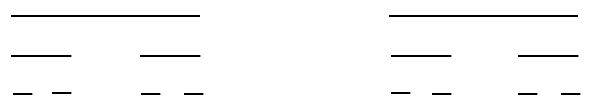
\includegraphics[width=0.75\textwidth]{image/CantorSet.jpg}
\vspace*{-0.3cm}
\caption{康托尔集的构造} \label{fig12}
\end{figure}

\noindent 令~$C = \smallcap^\infty \limits_{n=1} C_n$, 称为康托尔集\index{康托尔集}. 康托尔集具有以下性质:

\smallskip

(1) 康托尔集是闭的疏朗集(康托尔集无内点).

\smallskip

\begin{proof}
由闭集的性质易知康托尔集~$C$~是闭集. 为证~$C$~为疏朗集, 只需证明~$C^\circ = \emptyset$, 即任意~$C$~中的点都不是内点. 假设存在~$x \in C^\circ$, 则~$\exists~\varepsilon_0 > 0$, 使得~$(x-\varepsilon_0,\,x + \varepsilon_0) \subset C$. 取足够大的~$n_0$~使得~$1/3^{n_0} < \varepsilon_0$, 则~$(x-\varepsilon_0,\,x + \varepsilon_0)$~中必含有不属于~$C_{n_0}$~的点, 这与~$(x-\varepsilon_0,\,x + \varepsilon_0) \subset C = \smallcap\limits_{n=1}^\infty C_n$~矛盾.
\end{proof}

(2) 构造康托尔集从~$[0,\,1]$~中去掉的开区间长度之和为~$1$.

\smallskip

\begin{proof}
第~$n$~步, 去掉了~$2^{n-1}$~个长度为~$1/3^n$~的区间. 因此, 去掉的开区间长度之和为
\[
\sum^\infty _{n=1} \frac{2^{n-1}}{3^n} = \frac{1}{3}\sum^\infty _{n=1} \Big(\frac{2}{3}\Big)^{n-1} = 1
\]
\end{proof}

\smallskip

(3) 康托尔集是完全集(康托尔集每个点都是聚点).

\smallskip

\begin{proof}
设~$x \in C$, 则~$x \in C_n, \, n =1,\,2,\,\cdots$, 故对每个~$n \in \N$, $x$~属于长度为~~$1/3^n$~的闭区间
中的某一个, 记为~$F_n$. 于是, 对~$\forall~\varepsilon > 0$, 存在足够大的~$n_0$~使得~$1/3^{n_0} < \varepsilon$, 故~$F_{n_0} \subset U(x,\,\varepsilon)$. 又~$F_{n_0}$~的两个端点都属于~$C$, 故至少有一个端点不是~$x$, 记为~$x'$, 从而~$x' \in U(x,\,\varepsilon) \bigcap \big(C - \{x\}\big) \neq \emptyset$, 即~$x \in C'$.
\end{proof}

(4) $\overline{\overline{C}} = \overline{\overline{[0,\,1]}}$.

\smallskip

\begin{proof}
考虑~$[0,\,1]$~中的点用三进制小数表示. 去掉的开区间~$\big(1/3,\,2/3\big)$~
中的每个点~$x$~可表示为
\[
x = 0.1x_2x_3\cdots,\ \mbox{其中, } x_2,\,x_3,\,\cdots \in \{0,\,1,2\}
\]
区间端点~$1/3$~和~$2/3$~(属于~$C$)作特殊处理, 两种表示
\[
\frac{1}{3} = 0.100\cdots = 0.022\cdots, \quad \frac{2}{3} = 0.122\cdots = 0.200\cdots
\]
都采用后一种表示(不出现``1''). 去掉的开区间~$\big(1/9,\,2/9\big)$~
和~$\big(7/9,\,8/9\big)$~中
的点~$x$~可表示为
\[
x = 0.01x_3x_4\cdots \quad \mbox{~或~} \quad x = 0.21x_3x_4\cdots
\]
其中,  $x_3,\,x_4,\,\cdots \in \{0,\,1,2\}$. 区间端点~$1/9,\,2/9,\,7/9,\,8/9$~(属于~$C$)采用如下表示
\[
\frac{1}{9} = 0.0022\cdots, \quad \frac{2}{9} = 0.0200\cdots
\]
\[
\frac{7}{9} = 0.2022\cdots, \quad \frac{8}{9} = 0.2200\cdots
\]
依此类推, 去掉的开区间中的点必出现``1'', 而~$C$~则与所有不出现~``1''的小数一一对应, 即
\[
C \sim \big\{0.x_1x_2x_3\cdots: \: x_k \in \{0,\,2\}\big\}
\]
而
\[
\big\{0.x_1x_2x_3\cdots: \: x_k \in \{0,\,2\}\big\} \sim \big\{0.x_1x_2x_3\cdots: \: x_k \in \{0,\,1\}\big\}
\]
上式右端即为~$[0,\,1]$~的二进制小数表示, 故与~$[0,\,1]$~对等. 因此,
$\overline{\overline{C}} = \overline{\overline{[0,\,1]}}$.
\end{proof}

\begin{definition}
定义如下函数
\[
C(x)=\left\{\!\!
\begin{array}{cl}
0, & x = 0 \\[0.2cm]
\dfrac{2k-1}{2^n}, & x \in I_{n,k}  \\[0.2cm]
1, & x = 1
\end{array}
\right.
\]
其中, $I_{n,k}$($n=1,\,2,\,\cdots; \; k=1,\,\cdots, 2^{n-1}$)为康托尔集在构造过程中第~$n$~步挖去的
三分开区间, 该函数称为康托尔函数\index{康托尔函数}.
\end{definition}

康托尔函数~$C(x)$~是~$[0,\,1]$~上的单调递增的连续函数.

\newpage

\section*{附注~一}

\subsection*{实数的进制表示与转换}

下面介绍一下实数的~$p$~进制表示, $p \geqslant 2$~为整数. 首先回忆一下~$10$~进制表示
\[
256 = 2 \times 10^2 + 5 \times 10^1 + 6 \times 10^0
\]
\[
\pi = 3 \times 10^0 + 1 \times 10^{-1} + 4 \times 10^{-2} + \cdots
\]
\[
4.6799\cdots = 4.68
\]

类似地, 设~$x$~为一正实数, $p \geqslant 2$~为整数, 则~$x$~的~$p$~进制表示可以写成
\begin{eqnarray*}
x &=& b_m p^m + b_{m-1} p^{m-1} + \cdots + b_0 p^0 + a_1 p^{-1} + \cdots + a_n p^{-n} + \cdots \\
&=& \sum_{i=0} ^m b_i p^i + \sum_{j=1} ^\infty a_j p^j \\
&=& b_m b_{m-1} \cdots b_0.a_1 \cdots a_n \cdots
\end{eqnarray*}
其中, $b_i,\,a_j \in \{0,\,1,\,\cdots,\, p-1\}$. 若~$a_i$~从第~$i_0$~项之后都为~$p-1$, 而~$a_{i_0} \neq p-1$, 则把~$x$~表示为
\[
b_m b_{m-1} \cdots b_0.a_1 \cdots (a_{i_0}+1)
\]

上面的等式说明把~$x$~表示为一个正项级数, 其部分和~$S_{m+1+n}$~即为~$x$~的保留至第~$n$~位小数. 负实数~$y = - (-y)$, 则~$y$~的~$p$~进制表示即为正实数~$-y$~的~$p$~进制表示前面加负号. 因此, 每一个实数都可以
表示成~$p$~进制, 这也表明实数不同进制之间存在一一对应的关系.

$10$~进制转~$p$~进制算法:

\medskip

\begin{example}
$(14.267)_{10} = (~?~)_{3}$.
\end{example}

\begin{solution}
整数部分
\[
\left.
\begin{array}{l}
3~ | \! \underline{~14~~} \\[-0.2em]
~~3~ | \! \underline{~4~~} ~\cdots\cdots~ 2~ \quad b_0 \\[-0.2em]
~~\ 3~ | \! \underline{~1~} ~\cdots\cdots~ 1~ \quad b_1 \\[-0.2em]
~~~~~~~0~~\cdots\cdots~ 1~ \quad b_2
\end{array}
\right.
\quad \Longrightarrow \quad (14)_{10} = (112)_3
\]
小数部分
\[
\left.
\begin{array}{l}
~~0.267 \\[-0.3em]
\underline{\times ~~~~~3~} \\[-0.1em]
~~0.801 ~\cdots\cdots~ 0 ~\quad a_1 \\[-0.3em]
\underline{\times ~~~~~3~}  \\[-0.1em]
~~2.403 ~\cdots\cdots~ 2 ~\quad a_2 \\[-0.2em]
~~0.403 \\[-0.3em]
\underline{\times ~~~~~3~}  \\[-0.1em]
~~1.209 ~\cdots\cdots~ 1 ~\quad a_3 \\[-0.2em]
~~0.209 \\[-0.2em]
~~~~~\vdots ~~~~~~~~~~~~~~\vdots~~~~~\vdots
\end{array}
\right.
\quad \Longrightarrow \quad (0.256)_{10} = (0.021\cdots)_3
\]
故~$(14.267)_{10} = (112.021\cdots)_{3}$.
\end{solution}

$q$~进制转~$p$~进制算法: $q$~进制~$\rightarrow$~$10$~进制~~$\rightarrow$~$p$~进制.

\subsection*{集合悖论}

本章我们将集合定义为``具有确定内容或满足一定条件的事物的全体'', 这在历史上也曾被认为是一种满意的说法. 但在~20~世纪初, 英国逻辑学家罗素提出了下述悖论\footnote{悖论, 是指这样一个命题~$A$, 从~$A$~出发可以导出一个语句~$B$. 然而, 若假定~$B$~真, 则可推知~$B$~不真; 若假定~$B$~不真, 又推知~$B$~真. }
(也称为罗素悖论)
\begin{center}
``令~$X=\{E:\: E \in E\}$, 问集合~$X$~是否属于~$X$?''
\end{center}

该悖论给数学界带来了灾难性的后果! 它震撼了整个数学界乃至整个思想界, 从而促发了第三次数学危机.

\subsection*{集合论公理系统}

为了克服罗素悖论, 人们试图把集合论公理化, 用公理对集合加以限制.
第一个常用的公理系统是策梅洛和弗伦克尔等提出的~Z-F~集合论公理系统.
这个系统中只有一个非逻辑二元关系符号~``$\in$'', 非逻辑公理有: 外延公理、空集公理、无序对公理、并集公理、幂集公理、无穷公理、
分离公理模式、替换公理模式、正则公理, 再加上选择公理就构成~Z-F-C~系统.

利用公理可以定义出空集、序对、关系、函数等集合, 还可以给出序关系、良序关系、
序数、基数, 也可以给出自然数、整数、实数等概念. 集合论中有关集合的性质,
在公理集合论中都可以得到证明.\ 公理系统中还可以证明公理之间的相对和谐性和独立性,
例如, 柯恩于~1960~年创立公理集合论中的力迫法, 并用来证明~Z-F-C~系统与
连续统假设独立. 公理集合论发展很快, 马丁公理、苏斯林假设等新公理新方法已被广泛使用,
组合集合论、描述集合论、大基数、力迫法的研究已经渗透到数学的各个分支.

\subsection*{连续统假设}

关于无限集的基数, 我们知道最小的是可列集的基数~$\aleph_0$, 其次是实轴~$\R$~为代表的连续基数~$c$. 那么在~$\aleph_0$~和~$c$~之间是否还存在别的基数？这一问题曾耗费了康托尔本人不少的精力, 但并没有得出任何结论.

1900~年, 希尔伯特在巴黎数学家大会上提出了~23~个最重要的问题供~20~世纪的数学家们去研究, 这就是著名的``希尔伯特~23~个问题''. 其中列在首位的问题就是连续统假设

\begin{center}
``$\aleph_0$~与~$c$~之间不存在其他基数''
\end{center}

虽经后继者的许多努力, 也提出了若干等价的原则, 但还没有一个绝对的观念来说这一
猜测的真假. 不过在如今的~Z-F~集合论公理系统里, 哥德尔在~1940~年发表的文章中
证明了连续统假设的相容性(即连续统假设与~Z-F~集合论公理系统不矛盾). 而在~1963~年柯恩又证明了它的独立性(即连续统假设与~Z-F~集合论公理系统是相互独立的). 因此, 在目前最广泛采用的集合论公理系统中, 这一问题就算有了一个解答. 当然, 有的数学家认为: 应当有一个确定的集合理论出现, 使其中连续统假设是真或是假得到肯定回答.

\newpage

\begin{problemset}

\item 证明下列关于集合的关系式
\begin{enumerate}
\item[(1)] $A - (B-C) \subset (A-B) \cup C$.
\item[(2)] $(A-B)\cap (C-D) = (A \cap C)-(B \cup D)$.
\item[(3)] $A - (B - C) \subset (A - B) \cup C$. 问取~``=''~的充分必要条件是？
\item[(4)] 问~$A \cup (B-C) = (A \cup B) - C$~是否成立？
\end{enumerate}

\item 证明: $\{x : \: x>0\} = \smallcup\limits_{n=1}^\infty \big\{x: \: x > 1/n \big\}$.

\item 证明: $B - \limsup\limits_{n \to \infty} A_n = \liminf\limits_{n \to \infty} \big(B - A_n\big)$.

\item 设~$A_{2k-1} = \big(0,\, 1/k\big), \, A_{2k} = (0,\,k)$, $k=1,\,2,\,\cdots$, 求集列~$\{A_n\}$~的上限集和下限集.

\item 设当~$n$~为奇数时, $A_n = \big(0,\,1- 1/(n+2)\big)$; 当~$n$~为偶数时, $A_n = \big(1/n,\,1\big)$. 证明~$\lim\limits_{n \to \infty} A_n$~存在, 并求该极限.

\item 设~$f(x)$~为~$E$~上的实值函数, 则对任意的~$a \in \R$~有
\[
\big\{x \in E: \: f(x) > a \big\} = \medcup_{n=1}^\infty \Big\{ x \in E: \: f(x) > a+ \frac{1}{n} \Big\}
\]

\item 设~$\{f_n(x)\}$~为~$E$~上的实值函数列, 满足
\[
f_1(x) \leqslant f_2(x) \leqslant \cdots \leqslant f_n(x) \leqslant \cdots
\]
\[
\lim_{n \to \infty} f_n(x) = f(x)
\]
证明: 对任意~$a \in \R$, 都有
\[
\big\{ x \in E: \: f(x) > a \big\} = \medcup_{n =1}^\infty \big\{ x \in E: \: f_n(x) > a \big\}
\]

\item 设~$\{f_n(x)\}$~为~$E$~上收敛的实值函数列, 其极限函数记为~$f(x)$, 证明: 对~$\forall~a \in \R$~有
\[
\big\{x \in E: \: f(x) > a \big\} = \medcup_{k=1}^\infty \liminf_{n \to \infty} \Big\{x \in E: \: f_n(x) > a+\frac{1}{k} \Big\}
\]

\item 设~$X$~为全集, $A, \, A_\alpha \subset X, \, \alpha \in \mathnormal{\Gamma}$, 则
\begin{enumerate}
\item[(1)] $A = X$ $\Longleftrightarrow$ $\chi_A(x) = 1$;
\item[(2)] $A = \emptyset$ $\Longleftrightarrow$ $\chi_A(x) = 0$;
\item[(3)] $\chi_{\smallcup\limits_{\alpha \in \mathnormal{\Gamma}} A_\alpha} (x) = \max\limits_{\alpha \in \mathnormal{\Gamma}} \chi_{A_\alpha} (x)$;
\item[(4)] $\chi_{\smallcup\limits_{\alpha \in \mathnormal{\Gamma}} A_\alpha} (x) = \min\limits_{\alpha \in \mathnormal{\Gamma}} \chi_{A_\alpha} (x)$.
\end{enumerate}

\item 设~$\{A_n\}$~为集列, 证明\footnote{该结论表明: 集列的极限存在等价于函数列~$\{\chi_{\tiny{A_n}}(x)\}$~的极限存在. }
\[
\chi_{\limsup\limits_{n \to \infty} A_n}(x) = \limsup_{n \to \infty} \chi_{A_n}(x), \, \quad \chi_{\liminf\limits_{n \to \infty} A_n}(x) = \liminf_{n \to \infty} \chi_{A_n}(x)
\]

\item 证明: 单位圆周与整个实数轴对等.

\item 设~$\{A_n\}, \, \{B_n\}$~分别为两两互不相交的集列, 若~$A_n \sim B_n, \, n=1,\,2,\,\cdots$, 则对任意的~$N$~(有限或为~$+\infty$), 都有~$\smallcup\limits_{n=1}^N A_n \sim \smallcup\limits_{n=1}^N B_n$.

\item 设~$A_1 \smallcap A_2 = \emptyset, \, B_1 \smallcap B_2 = \emptyset$, 又~$\varphi_1:\:A_1 \rightarrow B_1,\, \varphi_2:\: A_2 \rightarrow B_2$~为两个一一映射, 若~$A_1 \subset A_2, \, B_1 \subset B_2$, 问是否存在~$A_2-A_1$~到~$B_2-B_1$~上的一一映射?

\item 用另一种方法证明定理~\ref{thm1.3.7}. (提示: 构造一一映射)

\item 证明: 有理数多项式全体构成的集合是可列集.

\item 证明: 平面上坐标为有理数的点组成的集合为可列集.

\item 设~$A$~为平面上以有理数点为中心, 以有理数为半径的圆的全体构成的集合, 则~$A$~为可列集.

\item 设~$B$~为自然数列的全体构成的集合, 问~$B$~与~$\N$~对等吗?

\item 设实轴上所有闭区间的全体构成的集合为~$E$, 则~$\overline{\overline{E}} = \aleph$.

\item 用~$\R^\infty = \big\{\{x_1, \, x_2, \, \cdots\}: \: x_i \in \R \big\}$~表示实数列的全体, 证明: $\overline{\overline{\R^\infty}} = \aleph$.

\item 用~$C[0,\,1]$~表示~$[0,\,1]$~上实值连续函数的全体,
      则~$\overline{\overline{C[0,\,1]}} = \aleph$.

\item 若~$\overline{\overline{\smallcup\limits_{n=1}^\infty A_n}} = \aleph$, 则必存在~$n_0$~使得~$\overline{\overline{A_{n_0}}} = \aleph$.

\item 证明: 设~$f(x)$~为~$(a,\,b)$~上的凸函数, 即对任意的~$x_1,\,x_2 \in (a,\,b)$~以及~$\lambda \in (0,\,1)$, 都有
\[
f\big(\lambda x_1+(1-\lambda)x_2 \big) \leqslant \lambda f(x_1) + (1- \lambda) f(x_2)
\]
则~$f(x)$~在除了一个至多可列集外的点上都是可微的.

\item 举例给出具有下列性质的点集:
\begin{enumerate}
  \item[(1)] $A_1$~只有一个极限点, 且极限点不属于~$A_1$;
  \item[(2)] $A_2$~有可列个极限点, 且极限点不属于~$A_2$;
  \item[(3)] 有边界点, 但边界点不属于该集合的平面点集;
  \item[(4)] 极限点一部分在集合中, 另一部分不在集合中, 甚至极限点比集合本身的点还要多.
\end{enumerate}

\item 设~$X = \R^2$~($xOy$~平面)为全集.

\begin{enumerate}
\item[(1)] $A = \{ (x,\,y): \: x^2 + y^2 < 1\}$, 求~$A',\, A^\circ,\,\overline{A}$;
\item[(2)] 设~$B = \{(x,\,y):\: x \in \R, \, y=f(x)\}$, 其中
\[
f(x) = \left\{ \!\!
\begin{array}{cl}
\sin \dfrac{1}{x}, & x \neq 0 \\[0.2cm]
0, & x=0
\end{array}
\right.
\]
求~$B',\,B^\circ$.
\end{enumerate}

\item 设~$A \subset \R^n$~为闭集, $B \subset \R^n$~为开集, 且~$A \subset B$, 则存在~$d > 0$~使得~$\smallcup\limits_{x \in A} U(x,\,d) \subset B$.

\item 设~$E \subset \R$~为可数集, 证明存在一点~$a \in \R$~使得~$E \cap \big(E + \{a\}\big) = \emptyset$.

\item 证明: 无理数的全体不能表示为可数个闭集的并.

\item 设~$f(x)$~为~$\R$~上的实值函数, 若~$f$~把任一开集映为开集,
      问~$f(x)$~是否连续? 又连续映射是否一定映开集为开集?

\item 设~$f(x)$~为~$\R$~上的连续函数, 证明对任意的~$a \in \R$:

\noindent (1) $\{x \in \R: \: f(x) > a\}$~与~$\{x \in \R: \: f(x) < a\}$~都是开集;

\noindent (2) $\{x \in \R: \: f(x) \geqslant a\}$~与~$\{x \in \R: \: f(x) \leqslant a\}$~都是闭集.

\item 设~$E$~为孤立点集, 问~$E$~上的任一函数是否连续? 是否一致连续?

\item 是否存在~$[0,\,1]$~上的函数, 满足它在每个有理数点不连续, 而在每个无理数点都连续?

\item 是否存在~$[0,\,1]$~上的函数, 满足它在每个有理数点都连续, 而在每个无理数点都不连续?
\end{problemset}

\chapter{勒贝格测度}

本章主要讨论~$\R$~中点集的测度理论, 先以第一章的``开集构造定理''为基础定义
一维有界开集、闭集的测度, 然后利用它们定义出~$\R$~中一般有界集的外测度与内测度,
进而给出~$\R$~中可测集的定义并讨论其性质. 另外, 简要介绍了~$\R^n$~中点集测度、波雷尔集以及不可测集的存在性.

回顾序章中介绍的勒贝格积分的大体思路, $f(x)$~在~$[a,\, b]$~上的勒贝格积分可定义为
\begin{equation} \label{eq20}
(L)\int_a ^b \!\! f(x) \mathrm{d}x = \lim_{\lambda \to 0} \sum^n _{i=1} \xi_i |E_i|
\end{equation}
其中, $\xi_i \in [y_{i-1},\,y_i]$
\[
E_i = \big\{ x \in [a,\,b]: \: y_{i-1} \leqslant f(x) < y_i \big\}
\]
$|E_i|$~表示一维集合~$E_i$~的``长度''.

可见, 建立勒贝格积分理论不可避免地要对~$\R^n$~中的一般点集给出类似于
一维区间长度的``适当的度量'', 为了测量~$\R^n$~中一般的集合的``大小''引入一种
适当的度量\raisebox{0.5mm}{-----}测度\index{测度}, 用~$m(\cdot)$~表示. 这种测度是长度、面积、
体积的推广, 并且要满足下列性质(以一维为例):

(i) (\textbf{非负性}) $m(E) \geqslant 0;$

(ii) (\textbf{有限可加性}) 若~$E_1 \cap E_2 = \emptyset$, 则
\[
m(E_1 \cup E_2) = m(E_1)+m(E_2)
\]

(iii) (\textbf{正则性}) $m\big([0,\,1]\big) = 1$.

以上三条性质又称为勒贝格测度公理.

\section{一维有界开集、闭集的测度}

\subsection{一维有界开集、闭集测度的定义}

\begin{definition}
设~$G \subset \R$~为有界开集, 由开集构造定理, $G = \smallcup\limits_k
(\alpha_k,\,\beta_k)$ ($k$~有限或可列, $(\alpha_k,\,\beta_k)$~为~$G$~的构成区间,
互不相交), 则
\[
m(G) = \sum_k (\beta_k - \alpha_k)
\]
称为一维有界开集~$G$~的测度\index{开集测度}.
\end{definition}

\begin{remark}
该定义要求~$m(G) < +\infty$, 即级数~$\sum\limits_{k=1}^\infty (\beta_k - \alpha_k)$~收敛.
$G$~有界, 则存在~$a,\,b \in \R$~使得~$G \subset (a,\,b)$.
又~$(\alpha_k,\,\beta_k)$~互不相交, 故对~$\forall~n \in \N$
\[
\sum^n _{k=1} (\beta_k - \alpha_k) \leqslant b-a
\]
令~$n \rightarrow \infty$, 得
\[
\sum^\infty_{k=1} (\beta_k - \alpha_k) \leqslant b-a < +\infty
\]
\end{remark}

\begin{definition}
设~$F \subset \R$~为有界闭集, 任取开区间~$(a,\,b) \supset F$,
令~$G = (a,\,b) - F$, 则~$G$~为~$\R$~中的有界开集
\[
m(F) = b - a - m(G)
\]
称为一维有界闭集~$F$~的测度\index{闭集测度}.
\end{definition}

\begin{remark}
(i) 对~$\forall~(a,\,b) \supset F$~都有~$m\big((a,\,b)-F\big) = b - a - m(F)$;

(ii) 上述定义中~$F$~的测度与开区间的选取无关;

(iii) $m\big( [a,\,b] \big) = b - a$.
\end{remark}

\begin{proof}
(i) 显然.

(ii) 若~$F$~为单点集. 设~$F = \{x\},\,x \in (a,\,b)$, 则~$G = (a,\,b) - \{x\}
= (a,\,x) \cup (x,\,b)$. 从而
\[
m(F) = b - a - m(G) = b -a -[(x-a)+(b-x)] = 0
\]

若~$F$~不是单点集. 令
\[
\alpha = \inf\{x: \: x\in F\},\quad \beta = \sup\{x: \: x\in F\}
\]
则~$\alpha \neq \beta$~且~$\alpha,\,\beta \in F$. 设~$F \subset (a,\,b),\,
G = (a,\,b) - F$, 则
\[
G = (a,\,\alpha) \cup (\beta,\,b) \cup \big( (\alpha,\,\beta) - F \big)
\]

\begin{figure}[!h]
\centering
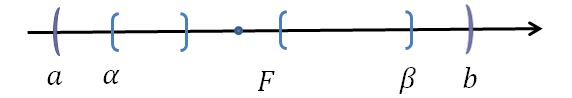
\includegraphics[width=0.5\textwidth]{image/ClosedSet.jpg}
\end{figure}

\noindent 故~$m(G) = \alpha - a + b - \beta + m\big( (\alpha,\,\beta) - F \big)$, 从而
\[
m(F) = b-a - m(G) = \beta - \alpha - m\big( (\alpha,\,\beta) - F \big)
\]

(iii) 由~(ii)~的证明知, $m\big([a,\,b]\big) = b - a - m\big( (a,\,b)
- [a,\,b] \big) = b - a$.
\end{proof}

\medskip

\begin{example}
求康托尔集的测度.
\end{example}

\medskip

\begin{solution}
记挖去的开区间全体为~$G_0$, 则~$G_0$~是~$\R$~中的有界开集, 故
\[
m(G_0) = \frac{1}{3} + \frac{2}{3^2} + \cdots + \frac{2^n}{3^{n+1}} + \cdots = 1
\]
从而~$m(C) = m\big([0,\,1]\big) - m(G_0) = 0$. 因此, 康托尔集是测度为~$0$~的不可列集.
\end{solution}

\subsection{一维有界开集测度的性质}

\begin{proposition} \label{prop221}
$\R$~中的有界开集测度具有如下性质:

(i) (\textbf{非负性}) $m(G) \geqslant 0$;

(ii) (\textbf{单调性}) 若~$G_1 \subset G_2$, 则~$m(G_1) \leqslant m(G_2)$;

(iii) (\textbf{次可加性}\index{次可加性}) 设~$k$~有限或可列
\[
m\big( \medcup_k G_k \big) \leqslant \sum_k m(G_k)
\]
\noindent 若~$G_k$~互不相交, 则
\[
m\big( \medcup_k G_k \big) = \sum_k m(G_k)
\]
\end{proposition}

\begin{proof}
(i) 显然.

(ii) 设~$G_1 = \smallcup\limits_k \big(\alpha^{(1)}_k,\,\beta^{(1)}_k\big),\,
G_2 = \smallcup\limits_k \big(\alpha^{(2)}_k,\,\beta^{(2)}_k \big)$, 则
\[
m(G_1) = \sum_k \big(\beta^{(1)}_k - \alpha^{(1)}_k\big), \quad m(G_2) =
\sum_k \big(\beta^{(2)}_k - \alpha^{(2)}_k\big)
\]
故对~$\forall~\varepsilon > 0$, 存在~$n_0 \in \N$~使得
\[
m(G_1) < \sum^{n_0}_{k=1} \big(\beta^{(1)}_k - \alpha^{(1)}_k\big) + \varepsilon
\]
由于~$G_1 \subset G_2$, 由命题~\ref{prop151}, $\big(\beta^{(1)}_k -
\alpha^{(1)}_k\big),\,k=1,\,\cdots,n_0$~必含于某~$m_0$~个~$G_2$~的构成区间
~$\big(\alpha^{(2)}_{k_j},\,\beta^{(2)}_{k_j} \big), j=1,\,\cdots,\,m_0$~
中($m_0 \leqslant n_0$), 故
\[
\sum^{n_0}_{k=1} \big(\beta^{(1)}_k - \alpha^{(1)}_k\big) \leqslant \sum^{m_0}_{j=1}
\big(\beta^{(2)}_{k_j} - \alpha^{(2)}_{k_j} \big)
\]
从而
\[
m(G_1) < \sum^{m_0}_{j=1} \big(\beta^{(2)}_{k_j} - \alpha^{(2)}_{k_j} \big) + \varepsilon \leqslant m(G_2) + \varepsilon
\]
由~$\varepsilon$~的任意性, $m(G_1) \leqslant m(G_2)$.

(iii) 不妨设~$\sum\limits_k m(G_k)<+\infty$, 否则显然成立.
记~$G = \smallcup\limits_k G_k$~是开集, 设
\[
G_k = \medcup\limits_i \big(\alpha^{(k)}_i,\, \beta^{(k)}_i \big),\quad
G = \medcup_j (\alpha_j, \, \beta_j)
\]
则每个区间~$(\alpha_j, \, \beta_j)$~都是某些小区间~$\big(\alpha^{(k)}_i,\,
\beta^{(k)}_i \big)$~的并. 由于~$\big\{(\alpha_j, \, \beta_j)\big\}$~互不相交,
故当~$j$~不同时, 构成~$(\alpha_j,\,\beta_j)$~的小区间的并也互不相交.
于是, 对任意的~$0 < \varepsilon < (\beta_j - \alpha_j)/2$,
闭区间~$[\alpha_j+\varepsilon,\,\beta_j -\varepsilon]$~中每个点都是构成
~$(\alpha_j,\,\beta_j)$~的某个小区间~$\big(\alpha^{(k)}_i,\, \beta^{(k)}_i \big)$~的
内点, 即~$[\alpha_j+\varepsilon,\,\beta_j -\varepsilon]$~中每个点都被
某个小开区间~$\big(\alpha^{(k)}_i,\, \beta^{(k)}_i \big)$~覆盖. 由有限开覆盖定理,
这些小区间~$\big(\alpha^{(k)}_i,\, \beta^{(k)}_i \big)$~中的有限个小开区间就可以
覆盖~$[\alpha_j+\varepsilon,\,\beta_j -\varepsilon]$, 故
\begin{eqnarray*}
\beta_j - \alpha_j - 2 \varepsilon &\leqslant& m\Big( \mbox{有限个~}
\big(\alpha^{(k)}_i,\, \beta^{(k)}_i \big) \Big) \\
&\leqslant& m \Big( \mbox{构成~}(\alpha_j, \, \beta_j)\mbox{~的所有~}
\big(\alpha^{(k)}_i,\, \beta^{(k)}_i \big) \Big)
\end{eqnarray*}
令~$\varepsilon \to 0$, 得
\[
\beta_j - \alpha_j \leqslant m \Big( \mbox{构成~}(\alpha_j, \, \beta_j)\mbox{~的所有~}
\big(\alpha^{(k)}_i,\, \beta^{(k)}_i \big) \Big)
\]
从而对所有的~$j$~求和得到
\begin{eqnarray*}
m(G) &=& \sum_j (\beta_j - \alpha_j) \\
&\leqslant& m\Big( \medcup_k \medcup_i \big( \alpha^{(k)}_i,\, \beta^{(k)}_i \big) \Big) \\
&=& \sum_k \sum_i \big(\beta^{(k)}_i - \alpha^{(k)}_i \big) \\
&=& \sum_k m(G_k)
\end{eqnarray*}

若~$\{G_k\}$~互不相交, 则每个~$(\alpha_j,\,\beta_j)$~正好是某一个
~$\big(\alpha^{(k)}_i,\, \beta^{(k)}_i \big)$. 此时
\[
m(G) = \sum_j(\beta_j - \alpha_j) = \sum_k \sum_i \big(\beta^{(k)}_i
- \alpha^{(k)}_i \big) = \sum_k m(G_k)
\]
\end{proof}

\subsection{一维有界闭集测度的性质}

\begin{proposition} \label{prop222}
$\R$~中的有界闭集测度具有如下性质:

(i) (\textbf{非负性}) $m(F) \geqslant 0$;

(ii) (\textbf{单调性}) 若~$F_1 \subset F_2$, 则~$m(F_1) \leqslant m(F_2)$.
\end{proposition}

\begin{proof}
(i) 设~$\alpha = \inf\{x: \: x\in F\},\,\beta = \sup\{x: \: x\in F\}$,
则开集~$(\alpha,\,\beta) - F \subset (\alpha,\,\beta)$. 由命题~\ref{prop221}~(ii)
\[
m\big( (\alpha,\,\beta) - F \big) \leqslant m\big( (\alpha,\,\beta) \big) = \beta - \alpha
\]
故~$m(F) = \beta - \alpha - m\big( (\alpha,\,\beta) - F \big) \geqslant 0$.

(ii) 设~$F_2 \subset (a,\,b)$, 由于~$F_1 \subset F_2$, 则开集~$(a,\,b) - F_2 \subset
(a,\,b) - F_1$. 由命题~\ref{prop221}~(ii), $m\big( (a,\,b) - F_2 \big) \leqslant
m\big( (a,\,b) - F_1 \big)$. 又
\[
m(F_1) = b-a - m\big( (a,\,b) - F_1 \big)
\]
\[
m(F_2) = b-a - m\big( (a,\,b) - F_2 \big)
\]
故~$m(F_1) \leqslant m(F_2)$.
\end{proof}

\begin{lemma} \label{lem223}
设~$F \subset \R$~为闭集, $G \subset \R$~为有界开集,
若~$F \subset G$, 则~$m(F) \leqslant m(G)$.
\end{lemma}

\begin{proof}
设~$G \subset (a,\,b)$, 由于~$F \subset G$, 则~$(a,\,b) = G \cup
\big( (a,\,b) - F \big)$. 由命题~\ref{prop221}~(iii)
\[
b - a = m\big((a,\,b)\big) \leqslant m(G) + m\big( (a,\,b) - F \big)
\]
又~$m(F) = b - a - m\big( (a,\,b) - F \big)$, 故~$m(F) \leqslant m(G)$.
\end{proof}

\begin{theorem} \label{thm221}
设~$G \subset \R$~为有界开集, 则~$m(G) = \sup\big\{m(F): \: F \subset G,\,
F \mbox{~闭}\big\}$.
\end{theorem}

\begin{proof}
由引理~\ref{lem223}, $\forall~F \subset G$, $F$~闭, 都有~$m(F) \leqslant m(G)$. 下
面证~$\forall~\varepsilon > 0$, 存在~$F_0 \subset G$,  $F_0$~闭, 使得
~$m(F_0) > m(G) - \varepsilon$.

设~$G = \smallcup\limits_k (\alpha_k,\,\beta_k)$, 则~$m(G) = \sum\limits_k(\beta_k -
\alpha_k)$. 故对上述~$\varepsilon$, 存在足够大的~$n_0$, 使得
\[
m(G) - \frac{\varepsilon}{2} < \sum^{n_0}_{k=1} (\beta_k - \alpha_k) < m(G) +
\frac{\varepsilon}{2}
\]
作
\[
[\alpha_k + \theta_k,\,\beta_k - \theta_k] \subset (\alpha_k,\,\beta_k),\quad
k=1,\,\cdots,\,n_0
\]
其中, $0< \theta_k < \min\big\{\varepsilon/4n_0,\,(\beta_k -
\alpha_k)/2 \big\}$. 令~$F_0 = \smallcup\limits_{k=1}^{n_0} [\alpha_k + \theta_k,\,\beta_k -
\theta_k]$, 则~$F_0$~闭, $F_0 \subset G$~且
\begin{eqnarray*}
m(F_0) &>& \sum^{n_0}_{k=1} \Big(\beta_k - \alpha_k - \frac{\varepsilon}{2n_0}\Big) \\
&=& \sum^{n_0}_{k=1} (\beta_k - \alpha_k) - \frac{\varepsilon}{2} \\
&>& m(G) - \varepsilon
\end{eqnarray*}
故定理结论成立.
\end{proof}

\begin{theorem} \label{thm222}
设~$F \subset \R$~为有界闭集, 则~$m(F) = \inf\big\{m(G): \: G \supset F,\,
G \mbox{~开}\big\}$.
\end{theorem}

\begin{proof}
由引理~\ref{lem223}, $\forall~G \supset F$, $G$~开, 都有~$m(F) \leqslant m(G)$.
取~$(a,\,b) \supset F$, 则~$(a,\,b) - F$~是有界开集. 由定理~\ref{thm221},
对~$\forall~\varepsilon > 0$, 存在闭集~$H \subset (a,\,b) - F$, 使得
\[
m\big((a,\,b) - F\big) < m(H) + \varepsilon
\]
即
\[
(b-a) - m(F) < m(H) + \varepsilon
\]
令~$G_0 = (a,\,b)-H$, 则~$G_0$~是开集, 满足
\[
F = (a,\,b) - \big[(a,\,b) - F\big] \subset (a,\,b) - H = G_0
\]
\[
m(G_0) = (b -a) - m(H) <  m(F) + \varepsilon
\]
故定理结论成立.
\end{proof}

\begin{proposition} \label{prop223}
设~$F_1,\,F_2,\,\cdots,\,F_n$~为~$\R$~中互不相交的有界闭集, 则
\[
m\Big( \medcup^n_{k=1} F_k \Big) = \sum^n_{k=1} m(F_k)
\]
\end{proposition}

\begin{proof}
只证~$n = 2$~的情形. 由定理~\ref{thm222}, 对~$\forall~\varepsilon > 0$,
存在有界开集~$G_1,\,G_2$~使得
\[
G_i \supset F_i, \quad m(G_i) < m(F_i) + \varepsilon, \quad i =1,\,2
\]
令~$G = G_1 \cup G_2$, 则~$G \supset F_1 \cup F_2$~且
\begin{eqnarray*}
m\big(F_1 \cup F_2\big) &\leqslant& m(G) \leqslant m(G_1) + m(G_2) \\
&<& m(F_1)+m(F_2) + 2\varepsilon
\end{eqnarray*}
由~$\varepsilon$~的任意性, $m\big(F_1 \cup F_2 \big) \leqslant  m(F_1)+m(F_2)$.

另一方面, $F_1,\,F_2$~闭, 且~$F_1 \cap F_2 = \emptyset$. 由定理~\ref{thm1413},
存在开集~$G_1,\,G_2$~使得~$F_1 \subset G_1, \, F_2 \subset G_2$, 且~$G_1 \cap G_2 =
\emptyset$. 又~$F_1 \cup F_2$~闭, 由定理~\ref{thm222}, 对~$\forall~\varepsilon > 0$,
存在有界开集~$G$~使得
\[
G \supset F_1 \cup F_2,\quad m(G) < m(F_1 \cup F_2) + \varepsilon
\]
注意到~$F_i \subset G_i \cap G,\,i=1,\,2$, 以及~$(G_1 \cap G) \cap (G_2 \cap G)
= \emptyset$. 则有
\begin{eqnarray*}
m(F_1) + m(F_2) &\leqslant& m(G_1 \cap G) + m(G_2 \cap G) \\
&=& m\big(G \cap (G_1 \cup G_2)\big) \\
&\leqslant& m(G) < m(F_1 \cup F_2) + \varepsilon
\end{eqnarray*}
由~$\varepsilon$~的任意性, $m(F_1)+m(F_2) \leqslant  m(F_1 \cup F_2)$.
\end{proof}

\begin{theorem} \label{thm223}
设~$F\subset \R$~为闭集, $G \subset \R$~为有界开集, 若~$F \subset G$, 则
\[
m(G-F) = m(G) - m(F)
\]
\end{theorem}

\begin{proof}
设~$G = \smallcup\limits_k (\alpha_k,\,\beta_k)$. 闭集~$F \subset G$, 由有限覆盖定理,
存在~$n$~使得~$F \subset \smallcup\limits_{k=1}^n (\alpha_k,\,\beta_k)$. 令
~$F_k = F \cap (\alpha_k,\,\beta_k), \, k = 1,\,\cdots,\,n$, 则~$F_k$~闭, 故
\[
m(F_k) = \beta_k - \alpha_k - m\big((\alpha_k,\,\beta_k) - F_k\big)
\]

\vspace*{-0.5cm}

\begin{figure}[!h]
\centering
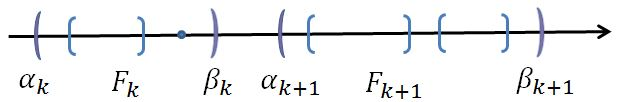
\includegraphics[width=0.5\textwidth]{image/ClosedSet2.jpg}
\end{figure}

\vspace*{-0.3cm}

注意到
\[
F = F \cap \big(\medcup\limits_{k=1}^n (\alpha_k,\,\beta_k)\big) =
\medcup\limits_{k=1}^n \big(F \cap (\alpha_k,\,\beta_k)\big) = \medcup\limits_{k=1}^n F_k
\]
由于~$\{F_k\}$~为互不相交的闭集, 由命题~\ref{prop223}
\begin{eqnarray} \label{eq221}
m(F) &=& m \Big(\medcup_{k=1}^n F_k \Big) = \sum_{k=1}^n m(F_k) \nonumber \\
&=& \sum_{k=1}^n (\beta_k - \alpha_k) - \sum_{k=1}^n m\big((\alpha_k,\,\beta_k)
- F_k\big) \\
&=& m(G) - \sum_{k=n+1}^\infty (\beta_k - \alpha_k) -
\sum_{k=1}^n m\big((\alpha_k,\,\beta_k) - F_k\big) \nonumber
\end{eqnarray}
并且
\[
G-F = \medcup\limits_{k=1}^n \big((\alpha_k,\,\beta_k) - F_k\big)
\medcup \big({\medcup\limits_{k=n+1}^\infty} (\alpha_k,\,\beta_k)\big)
\]
由于它们是互不相交的开集, 故由命题~\ref{prop221}
\begin{eqnarray} \label{eq222}
m(G-F) &=& m\big( \medcup_{k=1}^n \big((\alpha_k,\,\beta_k) - F_k\big) \big) +
m\big( \medcup_{k=n+1}^\infty (\alpha_k,\,\beta_k) \big) \nonumber \\
&=& \sum_{k=n+1}^\infty (\beta_k - \alpha_k) + \sum_{k=1}^n m\big((\alpha_k,\,\beta_k)
- F_k\big)
\end{eqnarray}
由式~\eqref{eq221},\,\eqref{eq222}~得, $m(G-F) = m(G) - m(F)$.
\end{proof}

\section{一维有界集的外测度、内测度}

\subsection{一维有界集的外测度}

\begin{definition}
设~$E \subset \R$~为有界集, 则~$E$~的外测度\index{外测度}定义为包含~$E$~的开集测度的下确界,
记为~$m^*(E)$, 即
\[
m^*(E) = \inf\big\{m(G): \: G \supset E,\, G \mbox{~开}\big\}
\]
\end{definition}

\begin{remark} \label{rem231}
(i) $E \subset \R$~有界, 则存在开区间~$(a,\,b) \supset E$,
即
\[
(a,\,b) \in \{G: \: G \supset E,\, G \mbox{~开}\}
\]
故~$m^*(E) \leqslant b - a < +\infty$. 从而上述定义有意义.

(ii) 任意一维有界集都有外测度, 若~$E$~是开集, 由开集测度的单调性
可得~$m^*(E) = m(E)$.
\end{remark}

\begin{theorem} \label{thm231}
设~$E \subset \R$~为有界集, 则存在单调递减开集列~$G_n$~满足~$G_n \supset E$,
且~$\lim\limits_{n \to \infty} m(G_n) = m^*(E)$.
\end{theorem}

\begin{proof}
$m^*(E) = \inf\{m(G): \: G \supset E,\, G \mbox{~开}\}$, 由~``$\inf$''~的定义,
对~$\varepsilon_1 = 1$, 存在开集~$G_1 \supset E$~使得
\[
m^*(E) \leqslant m(G_1) < m^*(E) + 1
\]
对~$\varepsilon_2 = 1/2$, 存在开集~$G'_2 \supset E$~使得
\[
m^*(E) \leqslant m(G'_2) < m^*(E) + \frac{1}{2}
\]
令~$G_2 = G'_2 \cap G_1$, 则~$G_2$~是开集, $G_2 \supset E$, 且
\[
m^*(E) \leqslant m(G_2) < m^*(E) + \frac{1}{2}
\]
依次做下去, 得到单调递减的开集列~$\{G_n\}$~满足~$G_n \supset E$, 且
\[
m^*(E) \leqslant m(G_n) < m^*(E) + \frac{1}{n}, \quad n = 1,\,2,\,\cdots
\]
两边取极限得~$m^*(E) = \lim\limits_{n \to \infty} m(G_n)$.
\end{proof}

\subsection{一维有界集外测度的性质}

\begin{proposition}[外测度性质]
设~$E,\,E_1,\,E_2,\,E_k$~为~$\R$~中的有界集, 则它们具有如下性质:

(i) (\textbf{非负性}) $m^*(E) \geqslant 0$;

(ii) (\textbf{单调性}) 若~$E_1 \subset E_2$, 则~$m^*(E_1) \leqslant m^*(E_2)$;

(iii) (\textbf{次可加性}) $m^*\big( \smallcup\limits_{k=1}^\infty E_k \big) \leqslant \sum\limits_{k=1}^\infty m^*(E_k)$.
\end{proposition}

\begin{proof}
(i), (ii)~显然.

(iii) 不妨设~$m^*(E_k) < +\infty, \, \forall~k \in \N$. 由外测度定义,
对~$\forall~\varepsilon > 0$, 存在开集~$G_k \supset E_k$~使得
\[
m(G_k) < m^*(E_k) + \frac{\varepsilon}{2^k}, \quad \forall~k \in \N
\]
令~$G = \smallcup\limits_{k=1}^\infty G_k$, 则~$G$~是开集, 且~$G \supset
\smallcup\limits_{i=1}^\infty E_k$. 故
\[
m^*\Big(\medcup^\infty_{k=1} E_k\Big) \leqslant m(G) \leqslant \sum^\infty_{k=1}m(G_k)
< \sum^\infty_{k=1} m^*(E_k) + \varepsilon
\]
由~$\varepsilon$~的任意性可得~$m^*\Big( \smallcup\limits_{k=1}^\infty E_k \Big) \leqslant
\sum\limits_{k=1}^\infty m^*(E_k)$.
\end{proof}

\medskip

\begin{example} \label{ex231}
若~$E$~是可数集, 则~$m^*(E) = 0$.
\end{example}

\medskip

\begin{proof}
不妨设~$E = \{x_n\}^\infty_{n=1}$, 对~$\forall~\varepsilon > 0$, 令
~$E_\varepsilon = \smallcup\limits_{n=1}^\infty \big(x_n-\varepsilon/2^{n+1},\,x_n+\varepsilon/2^{n+1}\big)$.
则~$E_\varepsilon$~是开集, 且~$E_\varepsilon \supset E$. 故
\[
m^*(E) \leqslant m(E_\varepsilon) = \sum_{n=1}^\infty \Big(2 \cdot
\frac{\varepsilon}{2^{n+1}} \Big) = \varepsilon
\]
由~$\varepsilon$~的任意性以及外测度的非负性得, $m^*(E) = 0$.
\end{proof}

\begin{theorem}
设~$E_1,\,E_2$~为~$\R$~中的有界集, 若~$d(E_1,\,E_2) > 0$, 则\footnote{外测度满足该定理条件, 也称其满足距离外测度性质. }
\[
m^*(E_1 \cup E_2) = m^*(E_1) + m^*(E_2)
\]
\end{theorem}

\begin{proof}
只需证明~$m^*(E_1) + m^*(E_2) \leqslant m^*(E_1 \cup E_2)$. 由外测度的定义,
对任意开集~$G \supset E$, $m^*(E)$~可表示为
\[
m^*(E) = \inf\{m(E'): \: E \subset E' \subset G, \, E' \mbox{~开}\}
\]
由于~$d(E_1,\,E_2)>0$, 由定理~\ref{thm1.4.10}, 则存在开集~$G_1,\,G_2$~
使得~$E_1 \subset G_1,\,
E_2\subset G_2$, 且~$G_1 \cap G_2 = \emptyset$. 从而
\begin{eqnarray*}
&& m^*(E_1)+m^*(E_2) \\
&=& \inf\big\{m(E'_1):\:E_1 \subset E'_1 \subset G_1,\, E'_1 \mbox{~开}\big\} + \inf\big\{m(E'_2):\:E_2 \subset E'_2 \subset G_2,\, E'_2 \mbox{~开}\big\} \\
&\leqslant& \inf\big\{m(E'_1)+m(E'_2):\:E_i \subset E'_i \subset G_i,\, E'_i \mbox{~开},
\,i=1,\,2\big\} \\
&=& \inf\big\{m(E'_1 \cup E'_2): \: (E_1 \cup E_2) \subset (E'_1 \cup E'_2) \subset
(G_1 \cup G_2),\,(E'_1 \cup E'_2) \mbox{~开}\big\} \\
&=& m^*(E_1 \cup E_2)
\end{eqnarray*}
定理得证.
\end{proof}

注意: 若定理条件减弱为~``$E_1 \cap E_2 = \emptyset$'', 则结论不一定成立.

\begin{theorem}[外测度平移不变性\index{外测度平移不变性}]
设~$E$~为~$\R$~中的有界集, $x_0 \in \R$, 则
\[
m^*\big(E + \{x_0\} \big) = m^*(E)
\]
\end{theorem}

\begin{proof}
若~$G$~是包含~$E$~的开集, 则~$G + \{x_0\}$~是包含~$E + \{x_0\}$~的开集,
且从~$G$~到~$G + \{x_0\}$~只是构成区间平移了~$x_0$~个单位, 区间长度并未发生变化.
由外测度的定义知定理结论成立.
\end{proof}

\subsection{一维有界集的内测度及性质}

\begin{definition}
设~$E \subset \R$~为有界集, 则~$E$~的内测度\index{内测度}定义为含于~$E$~的闭集测度的上确界,
记为~$m_*(E)$, 即
\[
m_*(E) = \sup \big\{m(F): \: F \subset E,\, F \mbox{~闭}\big\}
\]
\end{definition}

\begin{remark} \label{rem233}
任意一维有界集都有内测度, 若~$E$~是闭集, 由闭集测度单调性可得~$m_*(E) = m(E)$.
\end{remark}

\begin{proposition}
由内测度的定义, 易知~$\R$~上的内测度具有如下性质:

(i) (\textbf{非负性}) $m_*(E) \geqslant 0$;

(ii) (\textbf{单调性}) 若~$E_1 \subset E_2$, 则~$m_*(E_1) \leqslant m_*(E_2)$.
\end{proposition}

\begin{theorem}
设~$E \subset \R$~为有界集, 则存在单调递增闭集列~$F_n$~满足~$F_n \subset E$,
且~$\lim\limits_{n \to \infty} m(F_n) = m_*(E)$.
\end{theorem}

\begin{proof}
类似定理~\ref{thm221}~可证.
\end{proof}

\begin{proposition}
设~$E \subset \R$~为有界集, 则~$m_*(E) \leqslant m^*(E)$.
\end{proposition}

\begin{proof}
对任意有界开集~$G \supset E$, 闭集~$F \subset E$~都有~$F \subset E \subset G$,
故~$F \subset G$. 由引理~\ref{lem223}, $m(F) \leqslant m(G)$. 固定~$F$, 对~$G$~取~``$\inf$''~得
~$m(F) \leqslant m^*(E)$. 再对~$F$~取~``$\sup$''~得~$m_*(E) \leqslant m^*(E)$.
\end{proof}



\section{一维有界可测集及性质}

\subsection{一维有界可测集}

\begin{definition}
设~$E \subset \R$~为有界集, 若~$m_*(E) = m^*(E)$, 则称~$E$~为勒贝格可测集, 简称可测集\index{可测集}, 其测度记为~$m(E)$.
\end{definition}
\begin{remark}
一维有界开集、闭集都是可测集, 其测度就是~\S~2.1~中定义的测度.
\end{remark}

\begin{proof}
若~$G \subset \R$~为有界开集, 则由注~\ref{rem231}~和定理~\ref{thm221}~得~$m^*(G) = m(G) = m_*(G)$. 若~$F \subset \R$~为有界闭集,
则由注~\ref{rem233}~和定理~\ref{thm222}~得~$m_*(F) = m(F) = m^*(F)$.
\end{proof}

\begin{definition}
测度为~$0$~的集合, 称为零测集\index{零测集}.
\end{definition}

\begin{theorem}
零测集的任意子集可测, 且也是零测集.
\end{theorem}

\begin{proof}
设~$m(E) = 0, \, E_0 \subset E$, 则
\[
0 \leqslant m_*(E_0) \leqslant m^*(E_0) \leqslant m^*(E) = m(E) = 0
\]
故~$m(E_0) = m_*(E_0) = m^*(E_0) = 0$.
\end{proof}

\medskip

\begin{example}
设~$E$~是可数集, 则~$m(E) = 0$.
\end{example}

\medskip

\begin{proof}
由~\S~2.2~例~\ref{ex231}~知, $m^*(E) = 0$. 又~$0 \leqslant m_*(E) \leqslant m^*(E) =0$,
故~$m(E) = m_*(E) = m^*(E) =0$.
\end{proof}

\begin{theorem} \label{thm0}
可数个零测集的并是零测集.
\end{theorem}

\begin{proof}
设~$E_1,\,E_2,\,\cdots,\, E_n, \, \cdots$~是零测集, 记~$E = \smallcup\limits_{n=1}^\infty
E_n$. 由外测度定义, 对~$\forall~\varepsilon > 0$, 以及~$n \in \N$, 都存在开集~
$G_n \supset E_n$~满足
\[
m(G_n) < m^*(E_n) + \frac{\varepsilon}{2^n} = m(E_n) + \frac{\varepsilon}{2^n}
= \frac{\varepsilon}{2^n}
\]
令~$G = \smallcup\limits_{n=1}^\infty G_n$, 则~$G$~开, $G \supset E$, 且
\[
m^*(E) \leqslant m(G) \leqslant \sum_{n=1}^\infty m(G_n) < \varepsilon
\]
由~$\varepsilon$~的任意性, $m^*(E) = 0$, 从而~$m(E) = 0$.
\end{proof}

\begin{theorem} \label{thm242}
设~$E \subset \R$~为有界集, $E_0$~为零测集, 则:

(i) $m^*(E \cup E_0) = m^*(E)$;

(ii) $m_*(E \cup E_0) = m_*(E)$.
\end{theorem}

\begin{proof}
(i) 对~$\forall~\varepsilon > 0$, 取开集~$G \supset E,\,G_0 \supset E_0$~满足
\[
m(G) \leqslant m^*(E) + \frac{\varepsilon}{2}, \quad m(G_0) < \frac{\varepsilon}{2}
\]
则开集~$G \cup G_0 \supset E \cap E_0$, 且
\[
m(G \cup G_0) \leqslant m(G) + m(G_0) < m^*(E) + \varepsilon
\]
由~$\varepsilon$~的任意性, $m(G \cup G_0) \leqslant m^*(E)$, 再由外测度的定义
\[
m^*(E \cup E_0) \leqslant m(G \cup G_0) \leqslant m^*(E)
\]
而相反的不等式显然, 因此, $m^*(E \cup E_0) = m^*(E)$.

(ii) 设~$\varepsilon,\,G_0$~如~(i)~所述, 任取闭集~$F \subset E \cup E_0$, 则
\begin{eqnarray*}
m_*(F) &=& m_*\big((F - G_0) \cup G_0 \big) \leqslant m^*\big((F - G_0) \cup G_0 \big) \\
&\leqslant& m^*(F - G_0) + m^*(G_0)
\end{eqnarray*}
注意到~$F$~闭, $F - G_0$~闭, 且~$F - G_0 \subset E$,\, $G_0$~开, 故它们都是可测集, 于是
\[
m(F) \leqslant m(F-G_0) + m(G_0) < m_*(E) + \frac{\varepsilon}{2}
\]
由~$\varepsilon$~的任意性, $m(F) \leqslant m^*(E)$, 对闭集~$F$~取~``$\sup$''~得
\[
m_*(E \cup E_0) \leqslant m_*(E)
\]
而相反的不等式显然, 因此, $m_*(E \cup E_0) = m_*(E)$.
\end{proof}

由定理~\ref{thm242}, 对于~$\R$~中任意有界集~$E$, 并上零测集~$E_0$~不改变~$E$~的外测度和内测度, 从而:

\begin{corollary}
$\R$~中有界集并上零测集不改变可测性, 即若~$E$~不可测, 则~$E \cup E_0$~也不可测;
若~$E$~可测, 则~$E \cup E_0$~也可测, 且~$m(E \cup E_0) = m(E)$.
\end{corollary}

\begin{theorem} \label{thm243}
设~$E$~为~$\R$~中的有界集, 则~$E$~可测, 当且仅当存在开集~$G \supset E$,
闭集~$F \subset E$, 使得~$m(G-F) < \varepsilon$.
\end{theorem}

\begin{proof}
``$\Rightarrow$''. $E$~可测, 则~$m^*(E) = m_*(E) = m(E)$, 故对~$\forall~\varepsilon > 0$,
存在开集~$G \supset E$, 闭集~$F \subset E$~使得
\[
m(G) < m^*(E) + \frac{\varepsilon}{2} = m(E) + \frac{\varepsilon}{2}
\]
\[
m(F) > m_*(E) - \frac{\varepsilon}{2} = m(E) - \frac{\varepsilon}{2}
\]
从而由定理~\ref{thm223}, $m(G-F) = m(G)-m(F) < \varepsilon$.

``$\Leftarrow$''. 设对~$\forall~\varepsilon > 0$, 存在开集~$G \supset E$,
闭集~$F \subset E$~
使得~$m(G-F) < \varepsilon$. 由定理~\ref{thm223}, $m(G) - m(F) < \varepsilon$. 又
\[
m(F) \leqslant m_*(E) \leqslant m^*(E) \leqslant m(G)
\]
故~$m^*(E) - m_*(E) < \varepsilon$. 由~$\varepsilon$~的任意性,
则有~$m^*(E) \leqslant m_*(E)$. 而~$m^*(E) \geqslant m_*(E)$~总成立, 故~$m^*(E) = m_*(E)$,
从而~$E$~可测.
\end{proof}

\subsection{一维有界可测集的性质}

设下文中出现的集~$E,\,E_1,\,E_2,\,E_k$~等都是一维有界集.

\begin{proposition}[非负性]
$m(E) \geqslant 0$.
\end{proposition}

\begin{proposition}[平移不变性]
$m\big(E + \{x_0\} \big) = m(E)$.
\end{proposition}

\begin{proof}
由于~$m(E) = m^*(E)$, 再由外测度平移不变性可得.
\end{proof}

\begin{proposition}[集运算封闭性Ⅰ] \label{prop242}

(i) 设~$X = (a,\,b)$~为全集, 若~$E$~可测, 则~$E^c$~可测;

(ii) 若~$E_1,\,E_2$~可测, 则~$E_1 \cup E_2,\,E_1 \cap E_2,\,
E_1 - E_2$~都可测; 若~$E_1 \cap E_2 = \emptyset$, 则~$m(E_1 \cup E_2) = m(E_1) + m(E_2)$.
\end{proposition}

\begin{proof}
(i) $E$~可测, 由可测集等价定义, 对~$\forall~\varepsilon > 0$,
存在开集~$G \supset E$~与闭集~$F \subset E$, 使得~$m(G-F) < \varepsilon$.

则~$G^c$~闭满足~$G^c \subset E^c$, $F^c$~开满足~$F^c \supset E^c$, 并且
\[
F^c - G^c = \big[(a,\,b)-F\big] - \big[(a,\,b)-G\big] = G - F
\]
故~$m(F^c - G^c) = m(G - F) < \varepsilon$. 由可测集等价定义, $E^c$~可测.

(ii) $E_1,\,E_2$~可测, 由定理~\ref{thm243}, 存在开集~$G_i$, 闭集~$F_i$, 使得
\[
G_i \supset E_i \supset F_i, \quad m(G_i - F_i) < \varepsilon, \quad i = 1,\,2
\]
令~$G = G_1 \cup G_2,\,F = F_1 \cup F_2$, 则~$G \supset (E_1 \cup E_2) \supset F$, 且
\[
G-F \subset (G_1 - F_1) \cup (G_2 - F_2)
\]
从而
\begin{eqnarray*}
m(G-F) &\leqslant& m\big( (G_1 - F_1) \cup (G_2 - F_2) \big) \\
&\leqslant& m(G_1 - F_1) + m(G_2 - F_2) \\
&<& 2 \varepsilon
\end{eqnarray*}
由定理~\ref{thm243}, $E_1 \cup E_2$~可测.

若~$E_1 \cap E_2 = \emptyset$, 则~$F_1 \cap F_2 = \emptyset$. 由命题~\ref{prop223}
\begin{eqnarray*}
m(E_1 \cup E_2) &\geqslant& m(F_1 \cup F_2) = m(F_1) + m(F_2) \\
&>& m(G_1) + m(G_2) - 2 \varepsilon \\
&\geqslant& m(E_1) + m(E_2) - 2 \varepsilon
\end{eqnarray*}
由~$\varepsilon$~的任意性, $m(E_1 \cup E_2) \geqslant m(E_1) + m(E_2)$. 另一方面
\begin{eqnarray*}
m(E_1 \cup E_2) &\leqslant& m(G_1 \cup G_2) \leqslant m(G_1) + m(G_2) \\
&<& m(F_1) + m(F_2) + 2 \varepsilon \\
&\leqslant& m(E_1) + m(E_2) + 2 \varepsilon
\end{eqnarray*}
由~$\varepsilon$~的任意性得
\[
m(E_1 \cup E_2) \leqslant m(E_1) + m(E_2)
\]
综上~$m(E_1 \cup E_2) = m(E_1) + m(E_2)$.

注意到~$E_1 \cap E_2 = \big(E_1^c \cup E_2^c\big)^c$, 故~$E_1 \cap E_2$~可测.
再由~$E_1 - E_2 = E_1 \cap E_2^c$~知, $E_1 - E_2$~可测.
\end{proof}

\begin{remark} \label{rem242}
设~$X = (a,\,b)$~为全集, $E \subset X$, 则~$m(E^c) = b-a - m(E)$.
\end{remark}

\begin{proof}
由命题~\ref{prop242}~(ii), $m\big( (a,\,b) \big) = m(E \cup E^c) = m(E) + m(E^c)$.
注意到~$m(E) < +\infty$, 故
\[
m(E^c) = m\big( (a,\,b) \big) - m(E) = b-a - m(E)
\]
\end{proof}

\begin{proposition}[单调性]
设~$E_1,\,E_2$~可测, 且~$E_1 \subset E_2$, 则~$m(E_1) \leqslant m(E_2)$.
\end{proposition}

\begin{proof}
由命题~\ref{prop242}~(ii), $E_2 - E_1$~可测. 又~$E_2 = E_1 \cup (E_2 - E_1)$~且
~$E_1 \cap (E_2 - E_1) = \emptyset$, 注意到测度的非负性, 再由命题~\ref{prop242}~(ii)~得
\[
m(E_2) = m(E_1) + m(E_2 - E_1) \geqslant m(E_1)
\]
\end{proof}

\begin{proposition}[集运算封闭性Ⅱ] \label{prop244}

(i) 设~$E_1,\,E_2,\,\cdots$~可测, 则~$\smallcup\limits_{k=1}^\infty
E_k$~可测, 且满足次可加性
\[
m\big( \medcup_{k=1}^\infty E_k \big) \leqslant \sum_{k=1}^\infty m(E_k)
\]
若~$E_k$~互不相交, 则
\[
m\big( \medcup_{k=1}^\infty E_k \big) = \sum_{k=1}^\infty m(E_k)
\]

(ii) 设~$E_1,\,E_2,\,\cdots$~可测, 则~$\smallcap\limits_{k=1}^{\infty}E_k$~可测.
\end{proposition}

\begin{proof}
(i) 设~$E_1,\,E_2,\,\cdots$~可测, 记~$E = \smallcup\limits_{k=1}^\infty E_k$.

若~$E_k$~互不相交, 由命题~\ref{prop242}~易知, 对~$\forall~n \in \N$,
都有~$\smallcup\limits_{k=1}^n E_k$~可测, 且~$m\big( \smallcup\limits_{k=1}^n E_k \big)
= \sum\limits_{k=1}^n m(E_k)$. 故对~$\forall~\varepsilon > 0$, 存在闭集
~$F \subset \smallcup\limits_{k=1}^n E_k$, 使得
\[
m(F) > m_*\big( \medcup\limits_{k=1}^n E_k \big) - \varepsilon = m\big( \medcup\limits_{k=1}^n E_k \big) - \varepsilon
\]
故
\[
m_*(E) \geqslant m(F) > m\big( \medcup_{k=1}^n E_k \big) - \varepsilon =
\sum_{k=1}^n m(E_k) - \varepsilon
\]
由~$\varepsilon$~的任意性, $m_*(E) \geqslant \sum\limits_{k=1}^n m(E_k)$. 令~$n \to \infty$~得
~$m_*(E) \geqslant \sum\limits_{k=1}^\infty m(E_k)$.

另一方面, 对~$\forall~\varepsilon > 0$~及每个~$k$, 作开集~$G_k \supset E_k$, 满足
\[
m(G_k) < m^*(E_k) + \frac{\varepsilon}{2^k} = m(E_k) + \frac{\varepsilon}{2^k}
\]
令~$G = \smallcup\limits_{k=1}^\infty G_k$, 则~$G$~开, 且~$G \supset E$. 故
\[
m^*(E) \leqslant m(G) \leqslant \sum_{k=1}^\infty m(G_k) < \sum_{k=1}^\infty m(E_k)
+ \varepsilon
\]
由~$\varepsilon$~的任意性, $m^*(E) \leqslant \sum\limits_{k=1}^\infty m(E_k)$.
综上再由~$m_*(E) \leqslant m^*(E)$~可得, $m(E) = \sum\limits_{k=1}^\infty m(E_k)$.

若~$E_k$~相交, 则
\[
E = E_1 \cup (E_2 - E_1) \cup (E_3 - E_2 - E_1) \cup \cdots
\]
可测.

(ii) $\smallcap\limits_{k=1}^\infty E_k = \big( \smallcup\limits_{k=1}^\infty
E_k^c \big)^c$~可测.
\end{proof}

\begin{proposition}[单调集列测度的极限性质\index{单调集列测度的极限性质}] \label{prop245}

(i) 设~$\{E_k\}$~为单调递增的可测集列, 则~$E =\smallcup\limits_{k=1}^\infty E_k$~可测, 且
\[
m\big( \lim_{k \to \infty} E_k \big) = m(E) = \lim_{k \to \infty} m(E_k)
\]

(ii) 设~$\{E_k\}$~为单调递减的可测集列, 则~$E = \smallcap\limits_{k=1}^\infty E_k$~可测, 且
\[
m\big( \lim_{k \to \infty} E_k \big) = m(E) = \lim_{k \to \infty} m(E_k)
\]
\end{proposition}

\begin{proof}
(i) 由命题~\ref{prop244}, $E$~可测. 又~$E$~可分解为如下互不相交集的并
\[
E = E_1 \cup (E_2 - E_1) \cup \cdots \cup (E_k - E_{k-1}) \cup \cdots
\]
由于
\[
m(E_k) = m\big((E_k - E_{k-1}) \cup E_{k-1}\big) = m(E_k - E_{k-1}) + m(E_{k-1})
\]
注意到~$m(E_{k-1}) < +\infty$, 故~$m(E_k - E_{k-1}) = m(E_k) - m(E_{k-1})$.
于是由命题~\ref{prop244}~得
\begin{eqnarray*}
m(E) &=& m(E_1) + \sum_{k=2}^\infty m(E_k - E_{k-1}) \\
&=& m(E_1) + \sum_{k=2}^\infty \big(m(E_k) - m(E_{k-1})\big) \\
&=& \lim_{k \to \infty} m(E_k)
\end{eqnarray*}

(ii) 设~$X = (a,\,b)$~为全集. $\{E_k\}$~单调递减, 则~$\{E_k^c\}$~单调递增.
又~$E^c = \smallcup\limits_{k=1}^\infty E_k^c$, 应用~(i)~得~$m(E^c) =
\lim\limits_{k \to \infty} m(E_k^c)$. 由注~\ref{rem242}~得
\[
b-a - m(E) = \lim\limits_{k \to \infty} \big( b-a - m(E_k) \big)
\]
因此, $m(E) = \lim\limits_{k \to \infty} m(E_k)$.
\end{proof}

\subsection{测度的另一种定义}

\begin{lemma} \label{lem241}
设~$E \subset (a,\,b)$, 则~$m_*(E) + m^*(E^c) = b-a$.
\end{lemma}

\begin{proof}
对~$\forall~\varepsilon > 0$, 取闭集~$F \subset E$~满足~$m(F) > m_*(E) - \varepsilon$.
又~$F^c$~开, 且~$F^c \supset E^c$, 故由注~\ref{rem242}~得
\[
m^*(E^c) \leqslant m(F^c) = b-a - m(F)
\]
从而~$m_*(E) + m^*(E^c) < b-a + \varepsilon$. 由~$\varepsilon$~的任意性,
$m_*(E) + m^*(E^c) \leqslant b-a$.

另一方面, 设~$X = (a,\,b)$~为全集, 不妨设既开又闭. 

对~$\forall~\varepsilon > 0$, 取开集~$G \supset E^c$~满足~$m(G) < m^*(E^c) + \varepsilon$. 
又~$G^c$~闭, 且~$G^c \subset E$, 故
\[
m_*(E) \geqslant m(G^c) = b-a - m(G)
\]
从而~$m_*(E) + m^*(E^c) > b-a - \varepsilon$. 由~$\varepsilon$~的任意性,
$m_*(E) + m^*(E^c) \geqslant b-a$.

综上可得~$m_*(E) + m^*(E^c) = b-a$.
\end{proof}

\begin{theorem} \label{thm244}
设~$E \subset \R$~为有界集, 则~$E$~可测~$\Leftrightarrow$~对任意点集~
$T \subset \R$, 都有
\begin{equation} \label{eq21}
m^*(T) = m^*(T \cap E) + m^*(T \cap E^c)
\end{equation}
\end{theorem}

\begin{proof}
``$\Rightarrow$''.\ 设~$T$~为~$\R$~中的有界点集,
对~$\forall~\varepsilon > 0$, 由外测度定义, 存在开集~$G \supset T$~
使得~$m(G) < m^*(T) + \varepsilon$. 由于~$G \cap E \supset T \cap E,\,
G \cap E^c \supset T \cap E^c$, 故
\[
m^*(T \cap E) \leqslant m^*(G \cap E) = m(G \cap E)
\]
\[
m^*(T \cap E^c) \leqslant m^*(G \cap E^c) = m(G \cap E^c)
\]
注意到~$G \cap E$~与~$G \cap E^c$~互不相交, 则有
\[
m(G \cap E) + m(G \cap E^c) = m\big( (G \cap E) \cup (G \cap E^c) \big) = m(G)
\]
从而
\begin{eqnarray*}
m^*(T) &>& m(G) - \varepsilon \\
&=& m(G \cap E) + m(G \cap E^c) - \varepsilon \\
&\geqslant& m^*(T \cap E) + m^*(T \cap E^c) - \varepsilon
\end{eqnarray*}
由~$\varepsilon$~的任意性, $m^*(T) \geqslant m^*(T \cap E) + m^*(T \cap E^c)$.

另一方面, 由外测度的次可加性
\begin{eqnarray*}
m^*(T) &=& m^*\big( T \cap (E \cup E^c) \big) \\
&=& m^*\big( (T \cap E) \cup (T \cap E^c) \big) \\
&\leqslant& m^*(T \cap E) + m^*(T \cap E^c)
\end{eqnarray*}

综上可得~$m^*(T) = m^*(T \cap E) + m^*(T \cap E^c)$.

\smallskip

``$\Leftarrow$''.\ 设~$X = (a,\,b)$~为全集, 取~$T = (a,\,b)$, 则由条件~\eqref{eq21}
\[
b - a = m^*\big( (a,\,b) \big) = m^*(E) + m^*(E^c)
\]
故由引理~\ref{lem241}, $m^*(E) = b - a - m^*(E^c) = m_*(E)$. 因此, $E$~可测.
\end{proof}

\begin{remark}
(i) 条件~\eqref{eq21}~又称为卡拉西尔德瑞条件\index{卡拉西尔德瑞条件}, 许多实变函数教材把
定理~\ref{thm244}~作为勒贝格可测集的原始定义;

(ii) 由引理~\ref{lem241}, 有界集~$E$~的内测度可以表示为:
$m_*(E) = b - a - m^*(E^c)$. 可见, 一维有界集~$E$~的内测度、测度
都可以用外测度来定义.
\end{remark}

\subsection{波雷尔集}

下面讨论~$\R$~中可测集\footnote{~这里不区分有界、无界, 一维无界集的测度定义见~\S2.4.}的构造问题, 即~$\R$~中哪些点集是可测的？能否对可测集给出一种相对直观的描述？

我们知道, 一维开集、闭集是可测集, 由命题~\ref{prop244}, 可列个开集的并(是开集)、可列个开集的交、可列个闭集的并、可列个闭集的交(是闭集)仍是可测集.

\begin{definition}
可列个开集的交, 称为~$G_\delta$~集\index{$G_\delta$~集}; 可列个闭集的并,
称为~$F_\sigma$~集\index{$F_\sigma$~集}.
可见~$G_\delta$~集的余集是~$F_\sigma$~集; $F_\sigma$~集的余集是~$G_\delta$~集.
\end{definition}

\medskip

\begin{example}
有理数点集~$\Q$~可表示为~$\smallcup\limits_{k=1}^\infty \{r_k\}$,
从而是~$F_\sigma$~集.
\end{example}

\medskip

\begin{example}
设~$f(x)$~为定义在开集~$G \subset \R$~上的实值函数, 则~$f(x)$~的连续点集
是~$G_\delta$~集.
\end{example}

\medskip

\begin{proof}
记~$\omega(x)$~为~$f$~在点~$x$~的振幅, 则~$f(x)$~在~$x = x_0$~处连续的充要条件\footnote{该结论的证明见第四章第~4~节. }是
~$\omega(x_0) = 0$. 故~$f(x)$~的连续点集可表示为
\[
\medcap_{k=1}^\infty \Big\{ x \in G: \: \omega(x) < \frac{1}{k} \Big\}
\]
由于~$\{ x \in G: \: \omega(x) < 1/k \}$~是开集, 故~$f(x)$~的连续点集是~$G_\delta$~集.
\end{proof}

\begin{definition}
由~$\R$~中的开集、闭集, 经过至多可列次``并、交、差''~的运算得到的集合,
称为波雷尔集\index{波雷尔集}.
\end{definition}

波雷尔集, 也可以用~$\sigma$-代数\index{$\sigma$-代数}的方式定义如下:


\begin{definition}
设~$\mathnormal{\Gamma}$~是由~$X$~的子集构成的集族, 且满足:

(i) $\emptyset \in {\mathnormal\Gamma}$;

(ii) 若~$A \in {\mathnormal\Gamma}$, 则~$A^c \in {\mathnormal\Gamma}$;

(iii) 若~$A_n \in {\mathnormal\Gamma}, \, n = 1,\,2,\,\cdots$, 则~$\smallcup
\limits_{n = 1}^\infty A_n \in {\mathnormal\Gamma}$.
则称~${\mathnormal\Gamma}$~是一个~$\sigma$-代数.
\end{definition}

由~$\sigma$-代数的定义易知:
\begin{publist}
\item[(1)] 若~$A_n \in {\mathnormal\Gamma}, \, n = 1,\,\cdots, \, m$, 则~$\smallcup
\limits_{n = 1}^m A_n \in {\mathnormal\Gamma}$;
\item[(2)] 若~$A_n \in {\mathnormal\Gamma}, \, n = 1,\,2,\,\cdots$, 则
\[
\medcap_{n = 1}^\infty A_n \in {\mathnormal\Gamma}, \quad \limsup_{n \to \infty} A_n \in {\mathnormal\Gamma},
\quad \liminf_{n \to \infty} A_n \in {\mathnormal\Gamma}
\]
\item[(3)] 若~$A,\,B \in {\mathnormal\Gamma}$, 则~$A - B \in {\mathnormal\Gamma}$;
\item[(4)] $X \in {\mathnormal\Gamma}$.
\end{publist}

设~${\mathnormal\Sigma}$~是由~$X$~的子集构成的集族, 包含~${\mathnormal\Sigma}$~的最小
\footnote{按集合包含关系: ${\mathnormal\Sigma}_1 \preccurlyeq {\mathnormal\Sigma}_2 \Leftrightarrow {\mathnormal\Sigma}_1
\subset {\mathnormal\Sigma}_2$. }~$\sigma$-代数, 称为由~${\mathnormal\Sigma}$~生成的~$\sigma$-代数.

由~$\R$~中所有开集构成的开集族所生成的~$\sigma$-代数, 称为波雷尔
集类, 记为~$\mathfrak{B}(\R)$. $\mathfrak{B}(\R)$~中的元素,
称为波雷尔集.

显然, 开集、闭集、$G_\delta$~集、$F_\sigma$~集都是波雷尔集; 波雷尔集的余集是波雷尔集;
波雷尔集的有限或可列交、并是波雷尔集; 波雷尔集的上、下限集是波雷尔集.

\begin{theorem}
任意波雷尔集都是可测集.
\end{theorem}

\begin{theorem} \label{thm246}
设~$E \subset \R$~可测, 则存在~$G_\delta$~集~$A$~以及~$F_\sigma$~集~$B$,
使得~$A \supset E \supset B$~且~$m(A) = m(E) = m(B)$.
\end{theorem}

\begin{proof}
设~$E$~可测, 由外测度定义, 对每个~$n \in \N$, 存在开集~$G_n \supset E$~使得
\[
m(G_n) < m^*(E) + \frac{1}{n} = m(E) + \frac{1}{n}
\]
令~$A = \smallcap\limits_{n=1}^\infty G_n$, 则~$A$~是~$G_\delta$~集. 由于~$E \subset
A \subset G_n$, 故由测度的单调性
\[
0 \leqslant m(A) - m(E) \leqslant m(G_n) - m(E) < \frac{1}{n}
\]
令~$n \to \infty$~得, $m(A) = m(E)$.

由内测度的定义, 对每个~$n \in \N$, 存在闭集~$F_n \subset E$~使得
\[
m(F_n) > m_*(E) - \frac{1}{n} = m(E) - \frac{1}{n}
\]
令~$B = \smallcup\limits_{n=1}^\infty F_n$, 则~$B$~是~$F_\sigma$~集. 由于~$F_n \subset
B \subset E$, 故由测度的单调性
\[
0 \leqslant m(E) - m(B) \leqslant m(E) - m(F_n) < \frac{1}{n}
\]
令~$n \to \infty$~得, $m(B) = m(E)$.
\end{proof}

\begin{remark}
从前面定理证明可看出, 若~$E$~可测, 则存在~$G_\delta$~集~$A$~以及~$F_\sigma$~集~$B$,
使得~$A \supset E \supset B$~且~$m(A) = m^*(E),\, m(B) = m_*(E)$.
\end{remark}

由定理~\ref{thm246}, $\R$~中的可测集~$E$~与某个~$G_\delta$~集以及
某个~$F_\sigma$~集只相差一个零测集. 反过来, 某个$G_\delta$~集或~$F_\sigma$~集
并上零测集仍是可测集. 因此, 我们得到~$\R$~中可测集的一种构造:

\begin{theorem}
可测集~$=$~波雷尔集~$\smallcup$~零测集.
\end{theorem}

那么是否存在不是波雷尔集的可测集呢? 回答是肯定的, 下面给出这样一个例子.

\begin{lemma} \label{lem232}
设~$f(x)$~为定义在~$E \subset \R^n$~上的实值函数, ${\mathnormal\Gamma}$~为~$\R^n$~中一些子集构成的~$\sigma$-代数且~$E \subset {\mathnormal\Gamma}$. 令
\[
\A=\{A \subset \R: \: f^{-1}(A) \in {\mathnormal\Gamma}\}
\]
则~$\A$~是~$\sigma$-代数.
\end{lemma}

\begin{proof}
(i) 由于~$f^{-1}(\R)=E \in {\mathnormal\Sigma}$, 故~$\R \in \A$.

(ii) 若~$A \in \A$, 则由~$f^{-1}(A^c)=E-f^{-1}(A)$~可知~$f^{-1}(A^c) \in {\mathnormal\Gamma}$, 从而~$A^c \in \A$.

(iii) 若~$\{A_k\}$~是~$\A$~中的集列, 即~$f^{-1}(A_k) \in {\mathnormal\Gamma}$. 则由
\[
f^{-1}\big( \medcup_{k=1}^\infty A_k \big) = \medcup_{k=1}^\infty f^{-1}(A_k)
\]
可得~$f^{-1}\big( \smallcup\limits_{k=1}^\infty A_k \big) \in {\mathnormal\Gamma}$, 从而~$\smallcup\limits_{k=1}^\infty A_k \in \A$.

\medskip

综上可证得~$\A$~是一个~$\sigma$-代数.
\end{proof}

\begin{corollary} \label{cor232}
设~$f(x)$~为~$\R$~上的连续函数, 若~$A$~是波雷尔集,
则~$f^{-1}(A)$~也是波雷尔集.
\end{corollary}

\begin{proof}
设~${\mathnormal\Gamma}$~为~$\R$~中的~$\sigma$-代数, $G$~是~$\R$~中的开集,
由~$f$~的连续性知, $f^{-1}(G)$~也是开集. 令
\[
\A=\{A: \: f^{-1}(A) \in {\mathnormal\Gamma}\}
\]
则
\[
f^{-1}(G) \in {\mathnormal\Gamma}
\]
从而~$G \in \A$. 由引理~\ref{lem232}~可得~$\A$~是~$\sigma$-代数, 由此知一切波雷尔集
都属于~$\A$. 因此, 若~$A$~是波雷尔集, 则~$f^{-1}(A) \in {\mathnormal\Gamma}$, 即~$f^{-1}(A)$~是波雷尔集.
\end{proof}

\medskip

\begin{example}[非波雷尔集的可测集]
设~$C(x)$~为~$[0,\,1]$~上的康托尔函数, 作函数
\[
\mathnormal{\Phi}(x)=\frac{1}{2}\big( x + C(x) \big), \quad  x \in [0,\,1]
\]
显然, $\mathnormal{\Phi}(x)$~是~$[0,\,1]$~上的严格单调递增的连续函数,
且~$\mathnormal{\Phi}(0)=0,\,\mathnormal{\Phi}(1)=1$. 记其反函数为~$\mathnormal{\Phi}^{-1}$, 则~$\mathnormal{\Phi}^{-1}$~也连续.

现在取~$[0,\,1]$~中的康托尔集~$C$, 并记在构造过程中每步挖去的中间三等分开区间为~$I_{n,k}$
($n=1,\,2,\,\cdots;\;k=1,\,2,\,\cdots,\,2^{n-1}$), 其长度为~$|I_{n,k}|$, 则~$\mathnormal{\Phi}(I_{n,k})$~是长度为~$|I_{n,k}|/2$~的开区间, 从而
\[
m \Big(\mathnormal{\Phi}\big( \medcup_{n=1}^\infty \medcup_{k=1}^{2^{n-1}} I_{n,k} \big) \Big) = \frac{1}{2}
\]
若令~$\mathnormal{\Phi}(C)=H$, 则有~$m(H)=1/2$.

令~$W$~为~$H$~中的不可测集, 并记~$\mathnormal{\Phi}^{-1}(W)=S$. 则由~$S \subset C$~知, $S$~是可测集, 但~$S$~不是波雷尔集, 否则根据推论~\ref{cor232}~可
得~$W$~也是波雷尔集, 从而是可测集, 矛盾.
\end{example}

\medskip

注: 本节~$\R$~中的波雷尔集的定义和结论, 都可以平移到~$\R^n$~中.

\section{关于测度的几点注记}

\subsection{一维无界集的测度}

\begin{definition}
设~$E \subset \R$~为无界集, 若~$E$~与任何开区间的交集是可测的,
则称~$E$~是可测的, 其测度定义为
\[
m(E) = \lim_{\alpha \to \infty} m\big( (-\alpha,\,\alpha) \cap E\big)
\]
\end{definition}

\begin{remark}
若~$E$~可测, 则上述极限恒存在, 可能有限, 也可能为~$+\infty$. 若~$E$~有界, 则上述极限
与~\S2.3~中一维有界集的测度一致.
\end{remark}

一维无界可测集与一维有界可测集具有完全类似的性质, 例如:

\begin{proposition}
设~$\{E_k\}$~为~$\R$~中的可测集列(有界或无界), 则~$\smallcup\limits_{k=1}
^\infty E_k$~可测; 若~$E_k$~互不相交, 则~$m\big( \smallcup\limits_{k=1}^\infty E_k\big) =
\sum\limits_{k=1}^\infty m(E_k)$.
\end{proposition}

\begin{proof}
记~$E = \smallcup\limits_{k=1}^\infty E_k$, 则对任意的开区间~$I$, 有
\[
E \cap I = \medcup_{k=1}^\infty (E_k \cap I)
\]
$E_k$~可测, 故~$E_k \cap I$~是含于~$I$~内的有界可测集. 由命题~\ref{prop244},
$\smallcup\limits_{k=1}^\infty (E_k \cap I)$~可测, 从而~$E \cap I$~可测, 再由定义知~$E$~可测.

若~$E_k$~互不相交, 取
\[
I = I_\alpha = (-\alpha,\,\alpha), \quad \alpha > 0
\]
则~$E_k \cap I_\alpha$~也互不相交, 由命题~\ref{prop244}~得
\[
m(E \cap I) = m \big(\medcup_{k=1}^\infty (E_k \cap I)\big) = \sum_{k=1}^\infty
m(E_k \cap I_\alpha)
\]
令~$\alpha \to \infty$, 得~$m(E) = \sum\limits_{k=1}^\infty m(E_k)$.
\end{proof}

\subsection{$\R^n$~中点集的测度}

\begin{definition}
设实数~$a_i < b_i,\,i=1,2,\,\cdots,\,n$, 则称~$\R^n$~中的点集
\[
\big\{(\xi_1,\,\xi_2,\,\cdots,\xi_n):\: a_i < \xi_i < b_i,\,i=1,\,\cdots,\,n\big\}
\]
为~$\R^n$~中的开矩体, 也可写为直积形式
\[
(a_1,\,b_1) \times (a_2,\,b_2) \times \cdots \times (a_n,\,b_n)
\]
通常用~$I,\,J$~表示, 矩体~$I$~的体积记为~$|I|$, 直径记为~$\mathrm{diam}(I)$, 则
\[
|I| = \mathop{\textstyle{\prod}}\limits_{i=1}^n(b_i - a_i), \quad \mathrm{diam}(I) = \Big(\mathop{\textstyle{\sum}}\limits_{i=1}^n (b_i - a_i)^2
\Big)^\frac{1}{2}
\]
类似地可定义闭矩体、半开半闭矩体.
\end{definition}

\begin{definition}
设~$E \subset \R^n$, 若存在可数个开矩体~$\{I_k\}$~使得~$E \subset \bigcup
\limits_k I_k$, 则称~$\{I_k\}$~是~$E$~的一个~$L$-覆盖. 定义
\[
m^*(E) = \inf \Big\{ \mathop{\textstyle{\sum}}\limits_k |I_k|: \: \{I_k\} \mbox{~为~$E$~的~$L$-覆盖} \Big\}
\]
为~$E$~的外测度. 若对~$E$~的任一~$L$-覆盖, 均有~$\sum\limits_k |I_k| = \infty$, 则
~$m^*(E) = \infty$, 否则~$m^*(E) < \infty$.
\end{definition}

可见, $\R^n$~中点集~$E$~的外测度, 就是包含~$E$~最小开矩体的``体积''.

\S2.2~中一维有界集的外测度具有的性质: 非负性、单调性、次可加性(分离可加性)、
平移不变性等, 推广到~$\R^n$~中点集的外测度仍然成立.

\begin{definition}
设~$E \subset \R^n$, 若对任意点集~$T \subset \R^n$~都有
卡拉西尔德瑞条件成立, 即
\[
m^*(T) = m^*(T \cap E) + m^*(T \cap E^c)
\]
则称~$E$~为勒贝格可测集, 简称可测集.
\end{definition}

\S2.3~中一维有界可测集具有的性质: 非负性、单调性、集运算封闭性、单调集列测度的极限性质等,
推广到~$\R^n$~中可测点集仍然成立.


\subsection{不可测集\index{不可测集}的例}

实际中所遇到的~$\R^n$~中的点集都是可测集, 遇到不可测集的机会极少. 但不可测集确实存在, 通常用它来构造各种反例. 例如, 用不可测集可以作出是勒贝格可测集, 但不是波雷尔集的例子.

为了简单, 我们只给出一维不可测集\index{不可测集}的例, 它是基于选择公理构造出来的. 下文将会用到勒贝格测度的平移不变性.

\begin{lemma} \label{lem251}
设~$E \subset \R$, 且~$m(E) > 0$, 则对任意的~$\eta \in (0,\,1)$, 都存在
开区间~$(\alpha,\,\beta)$~使得~$m\big(E \cap (\alpha,\,\beta) \big) >
\eta (\beta - \alpha)$.
\end{lemma}

\begin{proof}
由外测度定义, 对~$\forall~\eta \in (0,\,1)$, 存在开集~$G \supset E$~使得
\[
m(G) < m^*(E)/\eta = m(E) / \eta
\]
即~$\eta m(G) < m(E)$. 记~$G = \smallcup\limits_{k} (\alpha_k,\,\beta_k)$,
其中~$(\alpha_k,\,\beta_k)$~为~$G$~的构成区间, 则必存在某个
~$(\alpha_{k_0},\,\beta_{k_0})$~符合引理要求. 若不然, 则对每个~$k \in \N$,
都有~$m\big(E \cap (\alpha_k,\,\beta_k) \big) \leqslant \eta (\beta_k - \alpha_k)$. 从而
\begin{eqnarray*}
m(E) &=& m(E \cap G) = m \big( \medcup_k \big(E \cap (\alpha_k,\,\beta_k)\big) \big) \\
&=& \sum_k m\big(E \cap (\alpha_k,\,\beta_k)\big) \leqslant \sum_k \eta (\beta_k - \alpha_k) = \eta m(G)
\end{eqnarray*}
矛盾.
\end{proof}

\begin{lemma} \label{lem252}
设~$E \subset \R$, 且~$m(E) > 0$. 作点集
\[
E - E = \{x-y:\: x,\,y \in E\}
\]
则存在~$\delta > 0$, 使得~$(-\delta,\,\delta) \subset E - E$.
\end{lemma}

\begin{proof}
由引理~\ref{lem251}, 存在开区间~$(\alpha,\,\beta)$, 记为~$I$, 使得
\[
m\big(E \cap I \big) > \frac{3}{4}(\beta - \alpha) = \frac{3}{4} m(I)
\]
取~$\delta = (\beta-\alpha)/2 = m(I)/2$, 则符合引理要求.

事实上, 任取~$z \in (-\delta,\,\delta)$, 则~$|z| < m(I)/2$. 由于
\[
(E \cap I) \cup \big((E \cap I) + \{z\}\big) \subset I \cup \big(I + \{z\}\big)
\]
注意到
\[
m\big(I \cup (I + \{z\})\big) \leqslant m(I) + |z| < \frac{3}{2}m(I)
\]
则有~$(E \cap I) \cap \big((E \cap I)+\{z\}\big) \neq \emptyset$. 否则,
由测度的平移不变性
\begin{eqnarray*}
&& m\big( (E \cap I) \cup \big((E \cap I)+\{z\}\big) \big) \\
&=& m(E \cap I) + m\big((E \cap I) + \{z\}\big) \\
&=&2 m(E \cap I) > \frac{3}{2}m(I)
\end{eqnarray*}
矛盾.

于是, 可以取到一点~$x \in (E \cap I) \smallcap \big((E \cap I)+\{z\}\big)$. 从而
~$x \in E$~且~$x \in E + \{z\}$, 即存在~$y \in E$~使得~$x = y + z$. 因此
\[
z = x - y, \quad x,\,y \in E
\]
即~$z \in E - E$. 再由~$z$~的任意性知, $(-\delta,\,\delta) \subset E - E$.
\end{proof}

\begin{theorem}
一维不可测集是存在的.
\end{theorem}

\begin{proof}
对于~$\forall~x,\,y \in \R$, 定义二元关系
\[
x \sim y ~\Leftrightarrow~ x - y \in \Q
\]
则容易验证~$\sim$~是~$\R$~上的等价关系. 用这一等价关系将~$\R$~分成
两两互不相交的等价类. 根据选择公理\footnote{选择公理: 若~${\mathnormal\Sigma}$~是由互不相交的一些
非空集合构成的集族, 则存在集合~$X$, 是由~${\mathnormal\Sigma}$~的每个集合中恰取一元所构成. },
在每一类中取出且只取一点, 构成的集合记为~$E$.
下面证明~$E$~是不可测集.

假设~$E$~可测, 分两种情况:

(1) $m(E) > 0$.

由引理~\ref{lem252}, 存在~$\delta > 0$~使得点集~$E - E$~中含有区间
~$(-\delta,\,\delta)$. 故存在
\[
x \in (E - E) \cap \Q, \quad x \neq 0
\]
于是存在~$y,\,z \in E$~满足~$y - z = x \in \Q, \, y \neq z$. 这说明~$y \sim z$,
从而~$y$~和~$z$~属于同一个等价类. 这与~$E$~的构造矛盾.

(2) $m(E) = 0$.

记~$\Q = \{r_k\}_{k=1}^\infty$. 考虑~$E$~的可列个平移集~$E + \{r_k\}, \,
k=1,\,2,\,\cdots$, 则有
\[
\R = \medcup_{k=1}^\infty \big(E + \{r_k\}\big)
\]
由于~$m(E) = 0$, 由测度的平移不变性知, $m\big(E + \{r_k\}\big) = 0$,
从而由上式及定理~\ref{thm0}~得到~$\R$~是零测集. 矛盾.
\end{proof}

\begin{remark}
定理证明中构造点集~$E$~时, 若把在每个等价类中选取的点限制在区间~$[0,\,1)$~内,
则得到~$E$~是有界不可测集.
\end{remark}

\newpage

\section*{附注~二}

\subsection*{等价关系与等价类}

\begin{definition}
设~$\sim$~为非空集~$X$~上的二元关系, 且满足:

(i) (\textbf{自反性}) $x \sim x$;

(ii) (\textbf{对称性}) 若~$x \sim y$, 则~$y \sim x$;

(iii) (\textbf{传递性}) 若~$x \sim y, \, y \sim z$, 则~$x \sim z$.
则称~$\sim$~是定义在~$X$~上的一个等价关系.
\end{definition}

例如, $x \equiv y ~(\mathrm{mod~} 2)$~是~$\mathbb{Z}$~上的等价关系; 三角形相似、
全等都是等价关系.

给定非空集~$X$~和等价关系~$\sim$, 对每个~$x \in X$, 可以定义~$x$~的等价类
\[
[x] := \{y \in X: \: y \sim x\}
\]
显然, $x \in [x]$, $x$~称为等价类~$[x]$~的代表元. 等价类的全体称为~$X$~关于~$\sim$~的商集
\[
X/\sim ~:= \{[x]:\: x \in X\}
\]
每个等价类的基数都相同(记为~$\overline{\overline{[~\!\cdot~\!]}}$), 且满足
\[
\overline{\overline{X}}  ~=~ \overline{\overline{X/\sim}}  ~\times~
\overline{\overline{[~\!\cdot~\!]}}
\]
例如, 等价关系~$x \equiv y ~(\mathrm{mod~} 2)$~生成两个等价类
\[
[0] = \{\mbox{偶数集}\}, \quad [1] = \{\mbox{奇数集}\}
\]

\begin{proposition}
等价类具有如下性质:

(i) $x \sim y~\Leftrightarrow~[x] = [y]$;

(ii) 对~$\forall~x, \, y \in X$, 则~$[x] = [y]$~或~$[x] \cap [y]
= \emptyset$.
\end{proposition}

\begin{proof}
(i) ``$\Rightarrow$''. 任取~$z \in [x]$, 则~$z \sim x$. 又~$x \sim y$,
故由传递性~$z \sim y$, 从而~$z \in [y]$. 于是~$[x] \subset [y]$.
同理可证~$[y] \subset [x]$. 因此, $[x] = [y]$.

``$\Leftarrow$''. 设~$[x] = [y]$, 由于~$x \in [x]$, 故~$x \in [y]$, 从而~$x \sim y$.

(ii) 设~$x, \, y \in X$, 假设~$[x] \cap [y] \neq \emptyset$, 则存在~$z \in [x] \cap [y]$,
故~$z \in [x]$~且~$z \in [y]$. 从而~$z \sim x$~且~$z \sim y$. 再由~(i)~得~$[z] = [x],
\, [z] = [y]$. 因此, $[x] = [y]$.
\end{proof}


\subsection*{偏序集·佐恩引理}

\begin{definition}
对给定的集合~$X$, 若它的某些元之间可以建立如下二元关系~$\preceq$:

(i)\ $x \preccurlyeq x$; (自反性)

(ii)\ $x \preccurlyeq y, \, y \preccurlyeq x$, 则~$x = y$; (对称性)

(iii)\ $x \preccurlyeq y, \, y \preccurlyeq z$, 则~$x \preccurlyeq z$. (传递性)

则称二元关系~$\preccurlyeq$~为集合~$X$~中的一个偏序(也称半序), 定义了偏序的集合~$(X,\,\preccurlyeq)$~称为偏序集.
\end{definition}

注意, 偏序集中并不要求每两个元素之间都存在偏序关系, 即偏序集中不是任何两个元素都可以比较``大小''.

\begin{definition}
设~$(X,\,\preccurlyeq)$~为偏序集, 若对~$\forall~x,\,y \in X$, 关系式~$x \preccurlyeq y$~或~$y \preccurlyeq x$~必有一个成立, 则称~$X$~的一个全序集.
\end{definition}

可见, 全序集中任何两个元素都可以比较``大小''.

\medskip

\begin{example}
自然数集~$\N$~与区间~$[0,\,1]$~都是全序集.
\end{example}

\medskip

\begin{example}
设~$A$~为非空集, 记~$X=2^A$~为~$A$~的幂集, 则~$X$~中的元按照集合的包含关系~$\subset$~构成一个偏序集,
但不是全序集.
\end{example}

\medskip

\begin{definition}
设~$(X,\,\preccurlyeq)$~为偏序集, $A \subset X$, 若存在~$b \in A$~使得
\[
b \preccurlyeq x, \, \quad \forall~x \in A
\]
则称~$b$~为~$A$~的下界, 最``大''的下界~$\tilde{b}$, 称为~$A$~的下确界, 记为~$\inf A$. 即若对~$A$~的任一下界~$b$, 都有~$b \preccurlyeq \tilde{b}$. 类似地可定义上界和上确界.
\end{definition}

\begin{definition}
设~$(X,\,\preccurlyeq)$~为偏序集, $A \subset X$, 若存在~$b \in A$, 使得对~$x \in A$~有
\[
b \preccurlyeq x \quad \mbox{或者} \quad  x \mbox{~与~} b \mbox{~无关}
\]
则称~$b$~为~$A$~的极小元\footnote{等价地: 对~$\forall~x \in A$, 若~$x \leqslant b$, 则~$x = b$.}, 类似地可定义极大元.
\end{definition}

\begin{definition}
设~$(X,\,\preccurlyeq)$~为全序集, 若~$X$~的每个非空子集都有极小元, 则称偏序关系~$\preccurlyeq$~为良序,
称~~$(X,\,\preccurlyeq)$~为良序集.
\end{definition}

\begin{remark}
良序集的所有子集都是良序集; 良序集一定是全序集, 反之不然; 有限的全序集一定是良序集.
\end{remark}

\medskip

\begin{example}
自然数集~$\N$~是良序集, 但区间~$[0,\,1]$~不是良序集, 因为~$(0.5,\,0.6] \subset [0,\,1]$~没有极小元.
\end{example}

\medskip

\begin{theorem}[佐恩引理\index{佐恩引理}]
设~$X$~为非空偏序集, 若~$X$~的任一非空全序子集都有下界, 则~$X$~必存在极小元.
\end{theorem}

\subsection*{选择公理}

在某些命题的证明中, 经常需要在一些集合中选取元素, 那么这种做法是否行得通呢？这就涉及选择公理.

1904~年, 策梅洛提出了选择公理, 并用它证明了良序定理\footnote{任何集合~$X$, 都存在偏序关系~$\preccurlyeq$, 使得~$(X,\,\preccurlyeq)$~是良序集. }. 选择定理与良序定理、佐恩引理等是等价的.
这些等价命题在许多数学分支中均有着应用. 例如建立实数的哈梅尔基、本课程中
勒贝格不可测集的存在、泛函分析中的哈恩\raisebox{0.5mm}{--}巴拿赫延拓定理、拓扑学中乘积拓扑
空间紧性的吉洪诺夫定理等.

\begin{theorem}[选择公理\index{选择公理}]
若~${\mathnormal\Gamma}$~是由一些互不相交的非空集合构成的集族, 则存在集合~$X$~满足: 它是由~${\mathnormal\Gamma}$~中每一个集合中恰取一个元素所构成.
\end{theorem}

选择公理并不限制集合中的元素是什么, 它与~Z-F~集合论公理系统是相容(不矛盾)
且相互独立的.

对于每个确定的非空集合, 指定属于它自身的一个元素总是可以做到的, 如果这些集合的个数有限,
则一个一个指定就行了. 所以选择公理的关键在于: 对无限多个非空集合, 同时指定属于每个集合自身的一个元素.
因此, 在没有选择公理的情况下, 除非另有标准外, 一般不能保证这样的元素同时被指定.

为了更好地理解选择公理, 下面引用罗素曾经举过的一个通俗例子:


假定有无限多双鞋, 我们要从每一双鞋中选出一只左脚穿的鞋, 并将其总体构成一个
集合, 那么这个集合是存在的. 但若将鞋换成袜子, 情况就不同了, 因为袜子不分左右,
所以就没有任何标准可以在两只中取一只.


\newpage
\begin{problemset}

\item 设~$E \ne \emptyset$, 但~$E'  = \emptyset$, 能否断定~$E$~可测？

\item 若~$m(E)=0$, 是否一定有~$m(\overline{E})=0$?

\item 对任一开集~$G$, 是否一定有~$m(G) = m(\overline{G})$?

\item $\R$~中至少含有一个内点的集合~$E$~(假设~$E$~可测)的测度可否为零？

\item 证明: 区间~$(a,\,b),\,[a,\,b],\, (a,\,b]$~ 都是可测集, 且其测度为~$b-a$.

\item 设~$E$~为~$\R$~的真子集, 且~$m^*(E) > 0$, 问是否~$E$~中必含有区间？

\item 设开集~$G_1$~是开集~$G_2$~的真子集, 则是否一定有~$m(G_1) < m(G_2)$?

\item 设~$\mathbb{I}$~为~$[0,\,1]$~中全体无理数点构成的集合.

\begin{enumerate}
  \item[(1)] 求~$m(\mathbb{I})$;
  \item[(2)] 由内外测度的定义, 考察其测度与~$1$~任意接近的含于~$\mathbb{I}$~内的闭集, 以及包含~$\mathbb{I}$~的开集是怎样的?
\end{enumerate}

\item 如果把外测度的定义改为`` 有界集~$E$~的外测度是包含~$E$~的闭集测度的下确界''
是否合理？

\item 设~$E_1,\,E_2$~为~$\R$~中的有界可测集, 证明
\[
m(E_1 \cup E_2) + m(E_1 \cap E_2) = m(E_1) + m(E_2)
\]

\item $E$~为~$\R$~中的不可测集, $A$~为零测集, 问~$E \smallcap A$~与~$E \smallcap A^c$~是否可测？

\item 对于有界集~$E \subset \R$, 是否必有~$m^*(E) < +\infty$?

\item 设~$E \subset \R$~为无界可测集, 是否必有~$m(E) = +\infty$~或~$m(E) > 0$?

\item 设~$E = \smallcup\limits_{n=1}^\infty E_n$, 其中, $E_1 \subset E_2 \subset \cdots \subset E_n \subset \cdots$, 且~$m(E_n) < +\infty$, 问~$E$~是否有有限测度？能否有无穷测度？

\item 设~$E = \smallcap\limits_{n=1}^\infty E_n$, 其中, $E_1 \supset E_2 \supset \cdots \supset E_n \supset \cdots$, 且~$m(E_n) = +\infty$, 问~$E$~能否有无穷、有限、零测度？

\item 设~$E$~为~$\R$~中的任一集合, 定义
\[
\mu(E) = \left\{\!\!
\begin{array}{cl}
m, & \mbox{若~} E \mbox{~只含~} m \mbox{~个点($m$~为有限的数)} \\[0.2cm]
+\infty, & \mbox{若~} E \mbox{~为无穷点集}
\end{array}
\right.
\]
问~$\mu(\cdot)$~是否为~$\R$~上的一个外测度？

\item 设~$A_1,\,\cdots,\,A_k, \, k=1,\,\cdots,\,n$~是有限个互不相交的可测集, 且~$E_k \subset A_k$, 证明
\[
m^*\big(\smallcup\limits_{k=1}^n E_k \big) = \sum\limits_{k=1}^n m^*(E_k)
\]

\item 设~$E_1 \subset E_2 \subset \cdots \subset E_n \subset \cdots$, 且~$\smallcup\limits_{n=1}^\infty E_n$~有界, 证明
\[
m^*\big(\smallcup\limits_{n=1}^\infty E_n \big) = \lim\limits_{n \to \infty} m^*(E_n)
\]

\item 设~$E_1 \supset E_2 \supset \cdots \supset E_n \supset \cdots$, 且~$E_1$~有界, 证明
\[
m_*\big(\smallcap\limits_{k=1}^\infty E_n \big) = \lim\limits_{n \to \infty} m_*(E_n)
\]

\item 试作一闭集~$F \subset [0,\,1]$, 使得~$F$~中不含任何开区间, 且~$m(F)=1/2$; 进一步, 对任意正数~$\alpha \in (0,\,1)$, 能否让~$m(F) = \alpha$?

\item 在~$[0,\,1]$~中作开集~$G$, 使得~$\overline{G} =[0,\,1]$, 而~$m(G) = 1/2$.

\item 在~$[0,\,1]$~中作点集
\[
E = \{x \in [0,\,1]:\: x \mbox{~的十进制小数表示中只出现~9~个数字}\}
\]
问~$E$~的测度与基数是多少？

\item 作~$[0,\,1] \times [0,\,1]$~中的点集
\[
E = \{(x,\,y):\: x \mbox{~与~} y \mbox{~至少有一个是有理数}\}
\]
试求~$m(E)$.

\item (\textbf{测度的介值定理})\ 设~$E$~为~$\R$~中的可测集, 且~$m(E) > 0$, 则对任意的~$0 < c < m(E)$, 都存在有界可测集~$E_0 \subset E$~使得~$m(E_0)=c$.

\item 设~$E$~为~$\R$~中的可测集, 且~$m(E) > 0$, 则存在~$x \in E$~使得对~$\forall~\delta >0$, 都有
\[
m\big( E \cap (x-\delta,\,x+\delta) \big) > 0
\]

\item 设~$\{E_n\}$~为~$\R^n$~中的可测集列, 且~$\smallcup\limits_{n=1}^\infty E_n$~有界, 则
\begin{enumerate}
  \item $m\big( \liminf\limits_{n \to \infty} E_n \big) \leqslant \liminf\limits_{n \to \infty} m(E_n)$;
  \item $m\big( \limsup\limits_{n \to \infty} E_n \big) \leqslant \limsup\limits_{n \to \infty} m(E_n)$.
\end{enumerate}

\item 举例给出一列可测集~$\{E_n\}$, 含在一个有限区间内, 且~$\lim\limits_{n \to \infty} E_n$~存在, 但
\[
m\big( \limsup_{n \to \infty} E_n \big) \neq m\big( \liminf_{n \to \infty} E_n \big)
\]
\end{problemset}


\chapter{可测函数}

本章先给出可测空间、测度空间的概念, 首先
\[
\mbox{空间~} = \mbox{~集合~} + \mbox{~一定结构或运算}
\]
例如, 定义了线性运算的集合~$(X,\,+,\cdot)$, 称为线性空间\index{线性空间};\
定义了距离的集合~$(X,\,d)$, 称为距离空间\index{距离空间}.

\begin{example}
设~$X$~为非空集, $\T$~是~$X$~的子集族, 且满足

(i) $\emptyset, \, X \in \T$;

(ii) 若~$A_1,\,\cdots,\,A_m \in \T$, 则~$\smallcap\limits_{k=1}^m A_k \in \T$;

(iii) 若~$A_1,\,A_2,\,\cdots \in \T$, 则~$\smallcup\limits_{k=1}^\infty A_k \in \T$.

\noindent 则称~$\T$~是~$X$~上的一个拓扑, $\T$~中的元称为开集, $(X,\,\T)$~
称为拓扑空间\index{拓扑空间}.
\end{example}

\begin{definition}
设~$X$~为非空集, 若~$X$~的子集族~$\F$~是~$\sigma$-代数, 即:

(i) $\emptyset \in \F$;

(ii) 若~$A \in \F$, 则~$A^c \in \F$;

(iii) 若~$A_n \in \F, \, n = 1,\,2,\,\cdots$, 则~$\smallcup
\limits_{n = 1}^\infty A_n \in \F$.

\noindent 若~$\F$~为~$\sigma$-代数，则可以对~$\F$~中的元定义测度, $\F$~中的元称为~$\F$-可测集,
简称可测集. 此时, 称二元组~$(X,\,\F)$~为可测空间\index{可测空间}.
\end{definition}

\begin{definition}
设~$(X,\,\F)$~为可测空间, 在~$\F$~上定义测度记为~$\mu$, 则称三元组
~$(X,\,\F,\,\mu)$~为测度空间\index{测度空间}.
\end{definition}

通常用~$(\R^n,\,\F,\,\mu)$~表示勒贝格测度空间, 其中~$\F$~为
~$\R^n$~中的勒贝格可测集, $\mu$~表示勒贝格测度.

定义在测度空间上的函数可以自然产生出各种各样的集合. 为用测度论的方法研究这个函数, 特别是在定义勒贝格积分时, 必须要求这些集合是勒贝格可测集, 由此产生了可测函数的概念. 勒贝格可积函数首先必须是可测函数. 本章介绍可测函数的定义、性质及构造, 可测函数的几种收敛性以及著名的叶戈洛夫定理、卢津定理、里斯定理.

\section{可测函数及其性质}

\subsection{可测函数的概念}

\begin{definition}
设~$E$~为可测集, $f: \: E \to \R \cup \{\pm \infty\}$~为实值函数, 若对~$\forall~a \in \R$, 都有~$\{x \in E: \: f(x) > a\}$~是可测集, 则称~$f$~为可测函数
\footnote{设~$f$~为波雷尔集~$E$~上的实值函数, 若对~$\forall~a \in \R$, 都有~$\{x \in E: \: f(x) > a\}$~是波雷尔集, 则称~$f(x)$~为~$E$~上的波雷尔可测函数\index{波雷尔可测函数}.}\index{可测函数}.
\end{definition}

\begin{definition}[用可测空间描述可测函数]
设~$(X,\,\F)$~为可测空间, $E$~为可测集, $f: \: E \to \R \cup \{\pm \infty\}$~为实值函数, 若对~$\forall~a \in \R$, 都有~$\{x \in E: \: f(x) > a\} \in \F$, 则称~$f$~为~$\F$-可测函数.
\end{definition}

\begin{proposition}[可测函数的等价定义] \label{prop311}
\quad ~~~(i) $f$~可测;\

$\Leftrightarrow$ ~ (ii) ~$\forall~a \in \R,\,\{x \in E: \: f(x) \geqslant a\}$~是可测集;\

$\Leftrightarrow$ ~ (iii) ~$\forall~a \in \R,\,\{x \in E: \: f(x) < a\}$~是可测集;\

$\Leftrightarrow$ ~ (iv) ~$\forall~a \in \R,\,\{x \in E: \: f(x) \leqslant a\}$~是可测集;\

$\Rightarrow$ ~ (v) ~$\forall~a,\,b \in \R,\, a < b, \,\{x \in E: \: f(x) \in [a,\,b) \}$~是可测集.

若~$|f(x)| < +\infty$, 则~(i)-(v)~等价.
\end{proposition}

\begin{proof}
(i) $\Rightarrow$ (ii). $f$~可测, 则~$\forall~a \in \R, \, \{x \in E: \: f(x) > a\}$~是可测集, 故
\[
\{x \in E: \: f(x) \geqslant a\} = \medcap_{n=1}^\infty \Big\{x \in E: \: f(x) > a - \frac{1}{n} \Big\}
\]
是可测集.

(ii) $\Rightarrow$ (iii). $\{x \in E: \: f(x) < a\} = \{x \in E: \: f(x) \geqslant a\}^c$~可测.

(iii) $\Rightarrow$ (iv). $\{x \in E: \: f(x) \leqslant a\} = \bigcap\limits_{n=1}^\infty \{x \in E: \: f(x) < a + 1/n\}$~可测.

(iv) $\Rightarrow$ (i).  $\{x \in E: \: f(x) > a\} = \{x \in E: \: f(x) \leqslant a\}^c$~可测. 故~(i)-(iv)~等价.

$\Rightarrow$ (v). 由~(ii)~和~(iii)~得
\[
\{x \in E: \: a \leqslant f(x) < b\} = \{x \in E: \: f(x) \geqslant a\} \cap \{x \in E: \: f(x) < b\}
\]
是可测集.

若~$|f(x)| < +\infty$, 则~$\{x \in E: \: f(x) = + \infty\} = \emptyset$, 从而
\[
\{x \in E: \: f(x) \geqslant a\} = \medcup\limits_{n=1}^\infty \{x \in E: \: a \leqslant f(x) < n\} \cup \{x \in E: \: f(x) = + \infty\}
\]
是可测集.
\end{proof}

\begin{remark}
条件~(v)~中的``~$[a,\,b)$''~换成~$\R$~中任一波雷尔集, 结论仍成立.
\end{remark}

\begin{proposition}
设~$f$~可测, 则下列集合都是可测集
\[
\{x \in E: \: f(x) = a\}, \quad \{x \in E: \: f(x) < +\infty \}
\]
\[
\{x \in E: \: f(x) > -\infty \}, \quad \{x \in E: \: |f(x)| = +\infty \}
\]
\end{proposition}

\begin{proof}
利用命题~\ref{prop311}, 只需注意到下述事实
\[
\{x \in E: \: f(x) = a\} = \{x \in E: \: f(x) \leqslant a\} \cap \{x \in E: \: f(x) \geqslant a\}
\]
\[
\{x \in E: \: f(x) < +\infty\} = \medcup_{n=1}^\infty \big\{x \in E: \: f(x) < n\big\}
\]
\[
\{x \in E: \: f(x) > -\infty\} = \medcup_{n=1}^\infty \big\{x \in E: \: f(x) > -n \big\}
\]
\[
\{x \in E: \: |f(x)| = +\infty\} = \medcap_{n=1}^\infty \big\{x \in E: \: |f(x)| \geqslant n\big\}
\]
\end{proof}

\begin{example} \label{ex311}
由于零测集的任意子集都是零测集(可测), 故定义在零测集上的任何函数都是可测函数.
\end{example}

\begin{definition}
设~$E = \smallcup\limits_{i=1}^n E_i$, $E_i$~可测且互不相交, 若定义在~$E$~上的函数
~$f(x)$~在每个~$E_i$~上取常数值~$c_i$, 即~$f(x) = \sum\limits_{i=1}^n c_i \chi_{E_i} (x)$, 则称~$f(x)$~是~$E$~上的简单函数\index{简单函数}.
\end{definition}

\begin{example} \label{ex312}
简单函数是可测函数.
\end{example}

\begin{proof}
不妨设~$c_1 < c_2 < \cdots < c_n$, 对~$\forall~a \in \R$, 有
\[
\{x \in E: \: f(x) > a\} = \left\{\!\!
\begin{array}{cl}
\emptyset, & \quad \mbox{若~} a \geqslant c_n \\
E_n, & \quad \mbox{若~} c_{n-1} \leqslant a < c_n \\
E_n \cup E_{n-1}, & \quad \mbox{若~} c_{n-2} \leqslant a < c_{n-1} \\
\vdots & \qquad  \qquad \vdots \\
E_n \cup \cdots \cup E_2,  & \quad \mbox{若~} c_1 \leqslant a < c_2 \\
E, & \quad \mbox{若~} a < c_1
\end{array}
\right.
\]
均是可测集, 故~$f(x)$~可测.
\end{proof}

\begin{example}
狄利克雷函数
\[
D(x) = \left\{ \!\!
\begin{array}{ll}
1, & x \mbox{~为~} [0,\,1] \mbox{~上的有理数~} \\[0.1cm]
0, & x \mbox{~为~} [0,\,1] \mbox{~上的无理数~}
\end{array}
\right.
\]
是可测函数.
\end{example}

\begin{proof}
对~$\forall~a \in \R$, 有
\[
\{x \in [0,\,1]: \: D(x) > a\} = \left\{\!\!
\begin{array}{cl}
\emptyset, & \quad \mbox{若~} a \geqslant 1 \\[0.1cm]
\Q_{[0,1]}, & \quad \mbox{若~} 0 \leqslant a < 1 \\[0.1cm]
{[}0,\,1{]}, & \quad \mbox{若~} a < 0
\end{array}
\right.
\]
均是可测集, 故~$D(x)$~可测.
\end{proof}

\begin{example}
连续函数是可测函数.
\end{example}

\begin{proof}
设~$f$~是定义在可测集~$E$~上的连续函数, 对~$\forall~a \in \R$, 记~$E_a = \{x \in E: \: f(x) > a\}$, 下面证明~$E_a$~是可测集.

任取~$x_0 \in E_a$, 则~$f(x_0) > a$. 令~$\varepsilon = f(x_0) - a > 0$, 由~$f$~连续, 则~$\exists~\delta > 0$~使得, 当~$x \in U(x_0,\,\delta) \cap E$~时, 有
\[
a = f(x_0) - \varepsilon < f(x) < f(x_0) + \varepsilon
\]
故~$U(x_0,\,\delta) \cap E \subset E_a$. 令~$G = \smallcup\limits_{x \in E_a} U(x,\,\delta_x)$, 则~$G$~是开集, 且
\[
G \cap E = \big( \medcup_{x \in E_a} U(x,\,\delta_x) \big) \cap E = \medcup_{x \in E_a} \big( U(x,\,\delta_x) \cap E \big) \subset E_a
\]
\[
E_a \subset \big( \medcup_{x \in E_a} U(x,\,\delta_x) \big) \cap E = G \cap E
\]
故~$G \cap E = E_a$, 再由~$G \cap E$~是可测集, 故~$E_a$~是可测集.
\end{proof}

\begin{example}
单调函数是可测函数.
\end{example}

\begin{proof}
不妨设~$f$~是定义在可测集~$E$~上的单调递增函数, 记~$R(f)$~表示~$f$~的值域.
对~$\forall~a \in \R$, 有
\[
\{x \in E: \: f(x) \geqslant a\} = \left\{\!\!
\begin{array}{cl}
\emptyset & \quad \mbox{若对~}\forall~ y \in R(f), \, \mbox{都有~} a > y \\[0.1cm]
E, & \quad \mbox{若对~}\forall~ y \in R(f), \, \mbox{都有~} a < y \\[0.1cm]
{[}x_0,\,+\infty) \cap E, & \quad \mbox{若~} a \in R(f)
\end{array}
\right.
\]
(其中, $x_0 \in E$~满足~$f(x_0) = a$)~均是可测集, 故~$f(x)$~可测.
\end{proof}

\subsection{可测函数的性质}

\begin{definition}
若~$m\{x \in E: \: f(x) \neq g(x)\} = 0$, 则称函数~$f$~与~$g$~在~$E$~上几乎处处\index{几乎处处}相等, 也称~$f$~与~$g$~对等. 记为~$f(x) = g(x), \, \mathrm{a.e.~} x \in E$.

若~$m\{x \in E: \: |f(x)| = + \infty\} = 0$, 则称函数~$f$~在~$E$~上几乎处处有限.

若~$f(x) = 0, \, \mathrm{~a.e.~} x \in E$, 则称~$f(x)$~为~$E$~上的零函数\index{零函数}.
\end{definition}

\begin{proposition} \label{prop313}
(i) 设~$f(x)$~在~$E$~上可测, $E_0$~是~$E$~的可测子集, 则~$f|_{E_0}(x)$;

(ii) 设~$f(x)$~在~$E_k$~上可测, $E = \smallcup\limits_k E_k$, 则~$f(x)$~在~$E$~上可测.
\end{proposition}

\begin{proof}
(i) $\{x \in E_0: \: f(x) > a\} = \{x \in E: \: f(x) > a\} \cap E_0$.

(ii) $\{x \in E: \: f(x) > a\} = \smallcup\limits_k\{x \in E_k: \: f(x) > a\}$.
\end{proof}

\begin{proposition}
若~$f(x)$~在~$E$~上可测, $g(x) = f(x), \, \mathrm{a.e.~} x \in E$, 则~$g(x)$~在~$E$~上可测.
\end{proposition}

\begin{proof}
令
\[
E_1 = \{x \in E: \: g(x) = f(x)\}, \quad E_2 = \{x \in E: \: g(x) \neq f(x)\}
\]
则~$E = E_1 \cup E_2$~且~$m(E_2) = 0$, 从而$E_1$可测. 由命题~\ref{prop313}~(i), $g|_{E_1} = f|_{E_1}$~可测; 由本节的例~\ref{ex311}, $g|_{E_2}$~可测, 再由命题~\ref{prop313}~(ii), $g$~在~$E$~上可测.
\end{proof}

\begin{definition}
设~$f(x)$~为定义在~$E$~上的函数, 则
\[
f^+(x) = \max\{f(x),\,0\} = \left\{\!\!
\begin{array}{cl}
f(x), & f(x) \geqslant 0 \\[0.1cm]
0, & f(x) < 0
\end{array}
\right.
\]
\[
f^-(x) = \max\{-f(x),\, 0\} = \left\{\!\!
\begin{array}{cl}
0, & f(x) \geqslant 0 \\[0.1cm]
-f(x), & f(x) < 0
\end{array}
\right.
\]
分别称为~$f$~的正部\index{函数正部}和负部\index{函数负部}. 
\end{definition}

显然有~$f^+(x), \, f^-(x)$~均非负, 且
\[
|f(x)| = f^+(x) + f^-(x), \quad f(x) = f^+(x) - f^-(x).
\]

\begin{figure}[!htb]
\centering
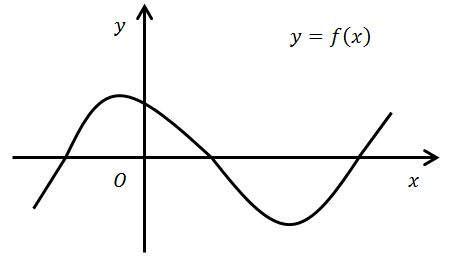
\includegraphics[width=0.31\textwidth]{image/yuanhanshu.jpg}
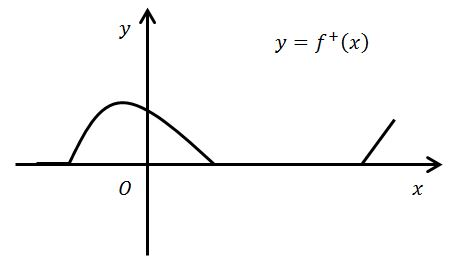
\includegraphics[width=0.31\textwidth]{image/hanshuzhengbu.jpg}
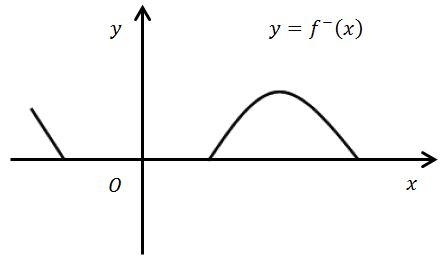
\includegraphics[width=0.31\textwidth]{image/hanshufubu.jpg}
\caption{~函数的正部与负部} \label{fig31}
\end{figure}

\begin{proposition}
设~$f(x),\,g(x)$~在~$E$~上可测, 则

(i) $f(x) \pm g(x), \, f(x)g(x), \, f(x)/g(x)$~均在~$E$~上可测;

(ii) $\max\{f(x),\,g(x)\}, \, \min\{f(x),\,g(x)\}$~均在~$E$~上可测;

(iii) $f^+(x), \, f^-(x), \, |f(x)|$~均在~$E$~上可测.
\end{proposition}

\begin{proof}
为了简单, 将~$\{x \in E: \: f(x) > a\}$~简记为~$E_{[f>a]}$.

(i) 对~$\forall~a \in \R$, 有~$E_{[f+g>a]} = E_{[f>a-g]}$. 任取~$x \in E_{[f>a-g]}$, 则~$f(x) > a - g(x)$. 由于有理数集~$\Q$~可列且在
~$\R$~中稠密, 则~$\exists~r_0 \in \Q$~使得
\[
f(x) > r_0 > a - g(x)
\]
故~$x \in E_{[f>r_0]}$~且~$x \in E_{[g>a-r_0]}$, 从而
\[
x \in \medcup\limits_{r \in \Q} \big( E_{[f>r]} \cap E_{[g>a-r]}\big)
\]
于是
\[
E_{[f>a-g]} \subset \medcup\limits_{r \in \Q} \big( E_{[f>r]} \cap E_{[g>a-r]}\big)
\]

反过来, 若存在~$r_0 \in \Q$~使得~$x \in  E_{[f>r_0]} \cap E_{[g>a-r_0]}$, 则
\[
f(x) > r_0, \quad g(x) > a - r_0
\]
故~$f(x) > r_0 > a - g(x)$, 从而~$x \in E_{[f>a-g]}$. 因此
\[
E_{[f>a-g]} =\medcup\limits_{r \in \Q} \big( E_{[f>r]} \cap E_{[g>a-r]}\big)
\]
$f,\,g$~可测保证上式右端是可测集, 从而~$f(x)+g(x)$~可测.

类似可证~$f(x)-g(x)$~可测.

先证~$f^2(x)$~可测. 由于
\[
E_{[f^2>a]} = \left\{
\begin{array}{cl}
E, & \quad \mbox{若~} a < 0 \\[0.1cm]
E_{[f>\sqrt{a}]} \cup E_{[f<-\sqrt{a}]}, & \quad \mbox{若~} a \geqslant 0
\end{array}
\right.
\]
是可测集, 故~$f^2(x)$~可测.

注意到
\[
f(x)g(x) = \frac{1}{4} \cdot \big[ \big( f(x) + g(x) \big)^2 - \big( f(x) - g(x) \big)^2 \big]
\]
故~$f(x)g(x)$~可测.

先证~$1/g(x)$~可测. 由于
\begin{eqnarray*}
E_{[1/g>a]} &=& E_{[g>0,g<1/a]} \medcup E_{[g<0,g>1/a]} \\
&=& \big(E_{[g>0]} \medcap E_{[g<1/a]} \big) \medcup \big(E_{[g<0]} \medcap E_{[g>1/a]} \big)
\end{eqnarray*}
是可测集, 故~$1/g(x)$~可测. 从而~$f(x)/g(x) = f(x)\cdot\big(1/g(x)\big)$~可测.

(ii) 由于
\[
E_{[\max\{f,g\}>a]} = E_{[f>a]} \medcup E_{[g>a]}, \quad E_{[\min\{f,g\}>a]} = E_{[f>a]} \medcap E_{[g>a]}
\]
故~$\max\{f(x),\,g(x)\}, \, \min\{f(x),\,g(x)\}$~可测.

(iii) 由~(ii)~以及~$f^+(x), \, f^-(x)$~的定义知, $f^+(x),\,f^-(x)$~可测. 再由~$|f(x)| = f^+(x) + f^-(x)$~及~(i)~知, $|f(x)|$~可测.
\end{proof}

\begin{proposition} \label{prop316}
设~$f_n(x), \, n = 1,\,2,\,\cdots$~在~$E$~上可测, 则
\[
\sup_n f_n(x),\quad \inf_n f_n(x),\quad \limsup_{n \to \infty} f_n(x), \quad \liminf_{n \to \infty} f_n(x), \quad \lim_{n \to \infty} f_n(x)
\]
均在~$E$~上可测.
\end{proposition}

\begin{proof}
由于
\[
\{x \in E: \: \sup_n f_n(x) > a\} = \medcup_{n=1}^\infty \{x \in E: \: f_n(x) > a\}
\]
\[
\{x \in E: \: \inf_n f_n(x) > a\} = \medcap_{n=1}^\infty \{x \in E: \: f_n(x) > a\}
\]
故~$\sup\limits_n f_n(x),\, \inf\limits_n f_n(x)$~可测. 又
\[
\limsup_{n \to \infty} f_n(x) = \inf_{k \geqslant 1} \big( \sup_{n \geqslant k}f_n(x) \big)
\]
故~$\limsup\limits_{n \to \infty} f_n(x)$~可测. 再由
\[
\liminf_{n \to \infty} f_n(x) = -\limsup_{n \to \infty} \big( -f_n(x) \big)
\]
故~$\liminf\limits_{n \to \infty} f_n(x)$~可测.

最后, 若~$\lim\limits_{n \to \infty} f_n(x)$~存在, 则
\[
\lim_{n \to \infty} f_n(x) = \limsup_{n \to \infty} f_n(x) = \liminf_{n \to \infty} f_n(x)
\]
也可测.
\end{proof}

\begin{remark}
我们知道, 连续函数的极限不一定是连续函数, 但由命题~\ref{prop316}, 可测函数的极限是可测函数, 这为处理一些问题带来极大的方便.
\end{remark}

\begin{proposition}
在~$\R$~上, 若~$g$~连续, $f$~可测, 则~$g \circ f$~可测.
\end{proposition}

\begin{proof}
对~$\forall~a \in \R$, 有
\[
\{x \in E: (g \circ f) (x) > a\} = (g \circ f)^{-1}(a,\,+\infty) = f^{-1} \big( g^{-1} (a,\, +\infty) \big)
\]
由于~$g$~连续, 故~$g^{-1} (a,\, +\infty)$~是开集, 记~$g^{-1} (a,\, +\infty) = \smallcup\limits_{k} (\alpha_k,\,\beta_k)$. 则
\begin{eqnarray*}
f^{-1} \big( g^{-1} (a,\, +\infty) \big) &=& f^{-1} \big( \medcup_{k} (\alpha_k,\,\beta_k) \big) = \medcup_{k} f^{-1} (\alpha_k,\,\beta_k) \\
&=& \medcup_{k}\{x \in E: \: \alpha_k < f(x) < \beta_k\} \\
&=& \big( \medcup_{k}\{x \in E: \: f(x) > \alpha_k \big\}) \medcap \big( \medcup_{k}\{x \in E: \: f(x) < \beta_k \big\})
\end{eqnarray*}
是可测集, 从而~$g \circ f$~可测.
\end{proof}

\begin{remark}
$f \circ g$~不一定可测, 从而两个可测函数的复合也不一定是可测函数. 绝对连续函数(\S 5.3)可将可测集映射为可测集, 然而严格单调的连续函数也不能将可测集映射为可测集
(可测函数更不能保证这一点). 例如, 设~$\varphi$~为~$[0,\,1]$~上的康托尔函数, 令
\[
h(x) = \frac{x + \varphi(x)}{2}
\]
则~$h: [0,\,1] \rightarrow [0,\,1]$~为严格递增的连续函数, 且~$m\big(h(C)\big)=1/2$, 其中~$C$~为康托尔集.
取~$W \subset h(C)$~为不可测集, 则~$M = h^{-1}(W)$~可测, 而~$h(M) = W$~不可测.

连续映射能保证波雷尔集的原象是波雷尔集, 但不能保证可测集的原象仍为可测集(可测函数更不能保证这一点). 例如, 前面的函数~$h$~为~$[0,\,1]$~到~$[0,\,1]$~的同胚映射\footnote{$h$~为一一映射, 且~$h$~与~$h^{-1}$~均连续.}, 易知其反函数~$h^{-1}$~在~$[0,\,1]$~也是严格递增的连续函数, 且可测集~$M$~在~$h^{-1}$~的原象~$W$~是不可测集.

进一步, 若记~$g = h^{-1}$~连续且严格递增, $W$~不可测, $g(W) = M$~可测. 令
\[
f = \chi_M(x), \quad x \in [0,\,1]
\]
则~$f$~可测. 由于
\[
\big\{ x \in [0,\,1]: \: f\big(g(x)\big) \neq 0 \big\} = \big\{ x \in [0,\,1]: \: g(x) \in M \big\} = W
\]
不可测, 故复合函数~$(f \circ g) = f\big(g(x)\big)$~不可测.
\end{remark}

\subsection{可测函数的构造}

简单函数只在有限个可测子集上取有限个实值, 从结构上来看是最简单的一类可测函数. 下面的定理将给出简单函数与一般可测函数的联系, 本书后面许多重要结果都是基于此得到的.

\begin{theorem}[可测函数构造定理\index{可测函数构造定理}] \label{thm311}
设~$f(x)$~为~$E$~上的非负可测函数, 则存在一列递增的非负简单函数~$\{ \varphi_n(x) \}$~满足~$\varphi_n \to f$(处处收敛),  即
\[
f(x) = \lim_{n \to \infty} \varphi_n(x), \quad \forall x \in E
\]
若~$f$~有界, 则~$\varphi_n \rightrightarrows f$(一致收敛).
\end{theorem}

\begin{proof}
(对值域做划分)对每个~$n \in \N$, 把~$[0,\,n]$~分为~$n^2$~等份, 即每段的长度是~$1/n$, 记
\[
E_{n,k} = \Big\{ x \in E: \: \frac{k-1}{n} \leqslant f(x) < \frac{k}{n} \Big\}, \quad k=1,\,\cdots,\, n^2
\]
\[
E_n = \{ x \in E: \: f(x) \geqslant n\}
\]

\begin{figure}[!htb]
\centering
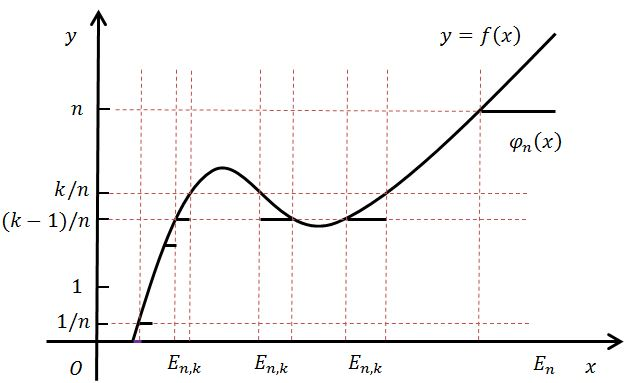
\includegraphics[width=0.8\textwidth]{image/kecehanshugouzao.jpg}
\vspace*{-0.2cm}
\caption{~可测函数的构造} \label{fig32} 
\end{figure}

注意到~$f$~在~$E$~上非负, 则有~$\big( \smallcup\limits_{k=1}^{n^2} E_{n,k} \big) \smallcup E_n = E$. 对~$\forall~x \in E$, 令
\[
\begin{array}{ll}
\varphi_n(x) = \left\{\!\!
\begin{array}{cl}
\dfrac{k-1}{n}, & x \in E_{n,k} \\[0.1cm]
n, & x \in E_n
\end{array}
\right.

\end{array}
\]
其中~$k = 1, \, \cdots, \, n^2$. 即
\[
\varphi_n(x) = \sum_{k=1}^{n^2} \frac{k-1}{n} \chi_{E_{n,k}}(x) + n \chi_{E_n}(x), \quad x \in E
\]

显然, $\varphi_n(x)$~是非负简单函数, 且
\[
\varphi_n(x) \leqslant \varphi_{n+1}(x) \leqslant f(x), \, \varphi_n(x) \leqslant n
\]
于是, 对~$\forall~x \in E$, 若~$f(x) < +\infty$, 则当~$n \geqslant f(x)$~时, 有
\[
0 \leqslant f(x) - \varphi_n(x) < \frac{1}{n}
\]
令~$n \to \infty$~得~$\lim\limits_{n \to \infty} \varphi_n(x) = f(x)$. 若~$f(x) = +\infty$, 则~$\varphi_n(x) = n, \, \forall~n \in \N$, 也有~$\lim\limits_{n \to \infty} \varphi_n(x) = f(x)$.

若~$f$~有界, 则存在~$M > 0$, 使得~$f(x) \leqslant M, \, \forall~x \in E$. 从而当~$n > M$~时, 有
\[
\sup_{x \in E} |f(x) - \varphi_n(x)| \leqslant \frac{1}{n}
\]
故~$\varphi_n \rightrightarrows f$.
\end{proof}

\begin{theorem} \label{thm312}
设~$f(x)$~为~$E$~上的可测函数, 则存在简单函数列~$\{ \varphi_n(x) \}$~满足
~$\varphi_n \to f$~且~$|\varphi_n(x)| \leqslant |f(x)|$. 若~$f$~有界, 则~$\varphi_n \rightrightarrows f$.
\end{theorem}

\begin{proof}
由于~$f(x) = f^+(x) - f^-(x)$, 则~$f^+(x),\,f^-(x)$~是非负可测函数. 由定理~\ref{thm311}, 存在简单函数列~$\{\varphi^{(1)}_n(x)\}, \{\varphi^{(2)}_n(x)\}$, 使得
\[
\lim_{n \to \infty} \varphi^{(1)}_n(x) = f^+(x), \quad \lim_{n \to \infty} \varphi^{(2)}_n(x) = f^-(x)
\]
令~$\varphi_n(x) = \varphi^{(1)}_n(x) - \varphi^{(2)}_n(x)$, 则容易验证~$\varphi_n(x)$~是简单函数, 且
\[
\lim_{n \to \infty} \varphi_n(x) = \lim_{n \to \infty} \big[\varphi^{(1)}_n(x) - \varphi^{(2)}_n(x) \big] = f^+(x) - f^-(x) = f(x)
\]
若~$f$~有界, 则~$f^+, \, f^-$~都有界, 由定理~\ref{thm311}, $\varphi^{(1)}_n \rightrightarrows f^+, \, \varphi^{(2)}_n \rightrightarrows f^-$, 从而
\[
\varphi_n = \varphi^{(1)}_n - \varphi^{(2)}_n \rightrightarrows f^+ - f^- = f
\]
定理得证.
\end{proof}

\begin{corollary}
$f$~可测~$\Leftrightarrow$~存在简单函数列~$\{ \varphi_n\}$~使得~$\varphi_n \rightarrow f$.
\end{corollary}

\begin{proof}
只需证充分性. 由于~$\varphi_n$~可测, 由命题~\ref{prop316}~知, $f(x) = \lim\limits_{n \to \infty} \varphi_n(x)$~可测.
\end{proof}

\section{可测函数列的收敛性}

可测函数列可以定义各种收敛性, 本节讨论几乎处处收敛、依测度收敛和接近一致收敛. 勒贝格定理、叶戈洛夫定理、里斯定理等揭示了几种收敛性之间的一些蕴含关系.

\subsection{几种收敛性}

\begin{definition}
设~$\{f_n(x)\}$~为~$E$~上的函数列, 对任意给定的~$x \in E$, 若对~$\forall~\varepsilon > 0$, $\exists~N_{\varepsilon,x} \in \N$, 使得当~$n \geqslant N_{\varepsilon,x}$~时, 有
\[
|f_n(x) - f(x)| < \varepsilon
\]
则称~$f_n(x)$~在~$E$~上处处收敛\index{处处收敛}\footnote{也称为点点收敛或收敛, 等价于~$\lim\limits_{n \to \infty} f_n(x) = f(x), \, \forall~x \in E$.}于~$f(x)$, 简记为~$f_n \rightarrow f$.
\end{definition}

\begin{definition}
设~$\{f_n(x)\}$~为~$E$~上的函数列, 若对~$\forall~\varepsilon > 0$,
$\exists~N_\varepsilon \in \N$, 使得当~$n \geqslant N_\varepsilon$~时, 有
\[
|f_n(x) - f(x)| < \varepsilon, \,\quad \forall~ x \in E
\]
或等价地, 若
\[
\lim_{n \to \infty} \sup_{x \in E} |f_n(x) - f(x)| = 0
\]
则称~$f_n(x)$~在~$E$~上一致收敛\index{一致收敛}于~$f(x)$, 简记为~$f_n \rightrightarrows f$.
\end{definition}

\begin{definition}
设~$\{f_n(x)\}$~为~$E$~上的函数列, 若存在零测集~$E_0 \subset E$, 使得~$f_n(x)$~在~$E - E_0$~上处处收敛于~$f(x)$, 则称~$f_n(x)$~在~$E$~上几乎处处收敛\index{几乎处处收敛}于~$f(x)$, 简记为~$f_n \xrightarrow{\mathrm{a.e.}} f$.
\end{definition}

\begin{remark}
在函数对等的意义下, 几乎处处收敛的极限函数是唯一的.
\end{remark}

\begin{proof}
设在可测集~$E$~上有~$f_n \xrightarrow{\mathrm{a.e.}} f,\, f_n \xrightarrow{\mathrm{a.e.}} g$. 则存在零测集~$E_1, \, E_2 \subset E$~使得
\[
f_n(x) \rightarrow f(x), \, \quad x \in E - E_1
\]
\[
f_n(x) \rightarrow g(x), \, \quad x \in E - E_2
\]
由于处处收敛的极限函数是唯一的, 故
\[
f(x) = g(x), \quad \forall~x \in E - (E_1 \cup E_2)
\]
注意到~$E_1 \cup E_2$~是零测集, 从而~$f(x) = g(x), \, \mathrm{~a.e.~} x \in E$.
\end{proof}

\begin{definition}
设~$\{f_n(x)\}$~为~$E$~上的函数列, 若对~$\forall~\varepsilon > 0$, 都有
\[
\lim_{n \to \infty} m\big( \{x \in E: \: |f_n(x) - f(x)| \geqslant \varepsilon\} \big) = 0
\]
或等价地,
若对~$\forall~\varepsilon > 0$~及~$\delta > 0$, 存在~$N_{\varepsilon,\delta} \in \N$, 使得当~$n \geqslant N_{\varepsilon,\delta}$~时, 有
\[
m\big( \{x \in E: \: |f_n(x) - f(x)| \geqslant \varepsilon\} \big) < \delta
\]
则称~$f_n(x)$~在~$E$~上依测度收敛\index{依测度收敛}于~$f(x)$, 简记为~$f_n \xrightarrow{~\mu~} f$.
\end{definition}

\begin{remark}
在函数对等的意义下, 依测度收敛的极限函数是唯一的.
\end{remark}

\begin{proof}
设在可测集~$E$~上有~$f_n \xrightarrow{~\mu~} f,\, f_n \xrightarrow{~\mu~} g$, 则对~$\forall k \in \N$, 有
\[
m(\{x \in E: |f_n(x) - f(x)| \geqslant \frac{1}{2k}\}) \to 0, \quad n \to +\infty
\]
\[
m(\{x \in E: |f_n(x) - g(x)| \geqslant \frac{1}{2k}\}) \to 0, \quad n \to +\infty
\]
对任意的~$n \in N$, 由于
\[
|f(x) - g(x)| \leqslant |f(x) - f_n(x)| + |f_n(x) - g(x)|
\]
故
\begin{eqnarray*}
&& \{x \in E: \: |f(x) - g(x)| \geqslant 1/k\} \\
&\subset& \Big\{x \in E: \: |f(x) - f_n(x)| \geqslant \frac{1}{2k} \Big\} \medcup \Big\{x \in E: \: |f_n(x) - g(x)| \geqslant \frac{1}{2k} \Big\}
\end{eqnarray*}
从而
\begin{eqnarray*}
	&& m(\{x \in E: \: |f(x) - g(x)| \geqslant 1/k\}) \\
	&\leqslant& m(\Big\{x \in E: \: |f(x) - f_n(x)| \geqslant \frac{1}{2k} \Big\}) + m(\Big\{x \in E: \: |f_n(x) - g(x)| \geqslant \frac{1}{2k} \Big\})
\end{eqnarray*}
令~$n \to \infty$, 可得~$m(\{x \in E: \: |f(x) - g(x)| \geqslant 1/k\})=0, \, \forall k \in \N$. 又
\[
\{x \in E: \: f(x) \neq g(x)\} = \medcup_{k=1}^\infty\{ x \in E: \: |f(x) - g(x)| \geqslant 1/k \}
\]
故
\[
m\big(\{x \in E: \: f(x) \neq g(x)\}\big) \leqslant \sum_{k=1}^\infty m(\{x \in E: \: |f(x) - g(x)| \geqslant 1/k\}) = 0
\]
因此，$f(x) = g(x), \, \mathrm{a.e.~} x \in E$.
\end{proof}

四种收敛间的关系: (前三个蕴含显然, 后一个蕴含见命题~\ref{prop321})
\[
f_n \rightrightarrows f ~ \Longrightarrow ~ f_n \rightarrow f ~ \Longrightarrow ~ f_n \xrightarrow{\mathrm{a.e.}} f \xLongrightarrow{m(E)<+\infty} f_n \xrightarrow{~\mu~} f
\]

\begin{example}[收敛但不一致收敛]
$f_n(x) = x^n, \, n=1,\,2,\,\cdots$~在~$[0,\,1]$~上处处收敛于
\[
f(x) = \left\{\!\!
\begin{array}{ll}
0, &  0 \leqslant x < 1 \\
1, &  x = 1
\end{array}
\right.
\]
但不一致收敛于~$f(x)$, 因为连续函数列的一致收敛极限必连续, 而~$f(x)$~不连续. 然而, 去掉任意小的一段之后
一致收敛, 即: 对~$\forall~\delta > 0$, $f_n(x)$~在~$[0,\,1-\delta]$~上一致收敛于~$0$.
\end{example}

\begin{example}[依测度收敛但不几乎处处收敛]
对每个~$n \in \N$, 都存在唯一的~$k,\,i \in \N$, 使得
\[
n = 2^k + i, \quad 0 \leqslant i < 2^k
\]
定义~$[0,\,1]$~上的函数
\[
f_n(x) = \chi_{[\frac{i}{2^k},\frac{i+1}{2^k})} (x), \quad n = 1,\,2,\,\cdots
\]
任取~$x_0 \in [0,\,1]$, 对每个~$k \in \N$, $\exists~0 \leqslant i_k < 2^k$~使得
\[
x_0 \in \big[\frac{i_k}{2^k},\frac{i_k+1}{2^k}\big)
\]
记~$n_k = 2^k + i_k$, 则
\[
f_{n_k}(x_0) = 1, \quad k = 1,\, 2,\,\cdots
\]
可见, $\{f_n(x_0)\}$~有无穷多项为~$1$, 无穷多项为~$0$. 故~$f_n(x)$~在~$[0,\,1]$~上每个点都不收敛(从而不是几乎处处收敛). 但对~$\forall~\varepsilon \in (0, \,1)$, 有
\[
m\big\{ x \in [0,\,1]: \: |f_n(x) - 0| \geqslant \varepsilon \big\} = \frac{1}{2^k} \to 0, \quad n \to \infty
\]
其中, $n = 2^k + i, \, 0 \leqslant i < 2^k$. 故~$f_n \xrightarrow{~\mu~} 0$. 这表明~$n$~越大, 出现~``~$1$''~的频率越趋于~$0$.
\end{example}

从几乎处处收敛与依测度收敛的定义来看, 几乎处处收敛是指在除去一个零测集~$E_0$~之外的每个点
~$x_0 \in E - E_0$~上, 其函数值数列~$\{f_n(x_0)\}$~都收敛;\
而依测度收敛是指函数列的不收敛点集~$\{x \in E: \: |f_n(x) - f(x)| \geqslant \varepsilon\}$~的测度是随着~$n$~的增大趋于~$0$~的.

\subsection{叶戈洛夫定理}

\begin{lemma} \label{lem321}
设~$\{f_n(x)\}$~为~$E$~上几乎处处有限的可测函数列, 且~$m(E) < +\infty$, 若~$f_n \xrightarrow{\mathrm{a.e.}} f$, 对~$\forall~\varepsilon > 0$, 令
\[
E_n(\varepsilon) = \big\{ x \in E: \: |f_n(x) - f(x)| \geqslant \varepsilon \big\}
\]
则有
\[
\lim_{N \to \infty} m \Big( \medcup_{n=N}^\infty E_n(\varepsilon) \Big) = 0
\]
\end{lemma}

\begin{proof}
由第一章~\S1.1~例~\ref{ex112}~的证明知, 对任意给定的~$\varepsilon > 0$, 上限集~$\mathop{\cap}\limits_{N=1}^\infty \mathop{\cup}\limits_{n = N}^\infty E_n(\varepsilon)$~中的点一定是不收敛点. 由于~$f_n \xrightarrow{\mathrm{a.e.}} f$, 故
~$m\big( \mathop{\cap}\limits_{N=1}^\infty \mathop{\cup}\limits_{n = N}^\infty E_n(\varepsilon) \big) = 0$. 注意到~$\big\{ \mathop{\cup}\limits_{n = N}^\infty E_n(\varepsilon) \big\}^\infty_{N=1}$~是单调递减集列, 由单调可测集列测度的极限性质可得
\[
\lim_{N \to \infty} m \big( \medcup_{n=N}^\infty E_n(\varepsilon) \big) =  m \big( \lim_{N \to \infty} \medcup_{n=N}^\infty E_n(\varepsilon) \big)= m\big( \medcap\limits_{N=1}^\infty \medcup\limits_{n = N}^\infty E_n(\varepsilon) \big) = 0
\]
引理证毕.
\end{proof}

\begin{theorem}[勒贝格定理\index{勒贝格定理}] \label{prop321}
设~$\{f_n(x)\}$~为~$E$~上几乎处处有限的可测函数列, 且~$m(E) < +\infty$, 若~$f_n \xrightarrow{\mathrm{a.e.}} f$, 则~$f_n \xrightarrow{~\mu~} f$.
\end{theorem}

\begin{proof}
由引理~\ref{lem321}, 对~$\forall~\varepsilon > 0$, 有
\[
\lim_{N \to \infty} m \big( \mathop{\cup}_{n=N}^\infty \big\{ x \in E: \: |f_n(x) - f(x)| \geqslant \varepsilon \big\} \big) = 0
\]
故由测度的单调性得
\begin{eqnarray*}
&& \lim_{n \to \infty} m\big( \{x \in E: \: |f_n(x) - f(x)| \geqslant \varepsilon \}\big) \\
&\leqslant& \lim_{n \to \infty} m \big( \mathop{\cup}_{k=n}^\infty \big\{ x \in E: \: |f_k(x) - f(x)| \geqslant \varepsilon \big\} \big) = 0
\end{eqnarray*}
从而, $f_n \xrightarrow{~\mu~} f$.
\end{proof}

\begin{remark}
勒贝格定理中条件~$m(E)< +\infty$~不能去掉. 例如, 取~$E = (0,\,+\infty)$, 令~$f_n(x) = \chi_{(0,n]}(x)$,
则
\[
f_n(x) \rightarrow f(x) \equiv 1, \quad x \in E
\]
但当取~$\delta = 1/2 >0$~时, 有
\[
m\big( \{x \in E: \: |f_n(x)-f(x)| \geqslant \delta\}\big) = m\big( (n,\, +\infty) \big) = +\infty
\]
故~$f_n$~不依测度收敛到~$f$.
\end{remark}

\begin{theorem}[叶戈洛夫定理\index{叶戈洛夫定理}]
设~$f_n(x),\,f(x)$~为~$E$~上几乎处处有限的可测函数, 且~$m(E) < +\infty$, 若~$f_n \xrightarrow{\mathrm{a.e.}} f$, 则对~$\forall~\delta > 0$, 存在~$E_\delta \subset E, \, m(E_\delta) < \delta$, 使得~$f_n(x)$~在~$E-E_\delta$~上一致收敛于~$f(x)$\footnote{也称~$f_n(x)$~在~$E$~上接近一致收敛于~$f(x)$.}.
\end{theorem}

\begin{proof}
由引理~\ref{lem321}, 对~$\forall~\varepsilon > 0$, 有
\[
\lim_{N \to \infty} m \big( \medcup_{n=N}^\infty E_n(\varepsilon) \big) = 0
\]
则对~$\forall~\delta > 0$, 以及每个~$k \in \N$, 都存在~$N_k$~使得
\[
m\Big( \medcup_{n = N_k}^\infty E_n\big( \frac{1}{k} \big) \Big) < \frac{\delta}{2^k}
\]
令~$E_\delta = \smallcup\limits_{k=1}^\infty \smallcup\limits_{n=N_k}^\infty E_n(1/k)$, 则
\[
m(E_\delta) \leqslant \sum_{k=1}^\infty m\Big( \medcup_{n=N_k}^\infty E_n\big( \frac{1}{k} \big) \Big) < \sum_{k=1}^\infty \frac{\delta}{2^k} = \delta
\]
下面证明~$f_n(x)$~在~$E - E_\delta$~上一致收敛于~$f(x)$. 注意到
\begin{eqnarray*}
E - E_\delta &=& E \cap E^c_\delta = E \cap \medcap\limits_{k=1}^\infty \medcap\limits_{n=N_k}^\infty E^c_n\Big( \frac{1}{k} \Big) \\
&=& \medcap\limits_{k=1}^\infty \medcap\limits_{n=N_k}^\infty \Big\{ x \in E: \: |f_n(x) - f(x)| < \frac{1}{k} \Big\}
\end{eqnarray*}
故只要~$x \in E - E_\delta$, 则对每一个~$k \in \N$, 都有
\[
x \in \medcap_{n=N_{k}}^\infty \Big\{ x \in E: \: |f_n(x) - f(x)| < \frac{1}{k} \Big\}
\]
于是, 对~$\forall~\varepsilon > 0$, 特别地, 取~$k_0 \in \N$~使得~$1/k_0 < \varepsilon$, 则
\[
x \in \medcap_{n=N_{k_0}}^\infty \Big\{ x \in E: \: |f_n(x) - f(x)| < \frac{1}{k_0} \Big\}
\]
即当~$n \geqslant N_{k_0}$~时, 有
\[
|f_n(x) - f(x)| < \frac{1}{k_0} < \varepsilon
\]
这说明~$f_n(x) \rightrightarrows f(x), \, \forall~x \in E - E_\delta$.
\end{proof}

\begin{remark}
(i) 条件~``~$m(E) < +\infty$''~不能少. 例如, 设~$E = (0,\,+\infty)$, 则~$m(E) = + \infty$. 作~$E$~上的函数列
\[
f_n(x) = \chi_{(0,\,n]} (x), \quad x \in E, \quad n = 1,\,2,\,\cdots
\]
则易知~$f_n(x)$~在~$E$~上处处收敛于~$1$. 但由于对~$\delta > 0$,
当~$m(E_\delta) < \delta$~时, 对每个~$n \in \N$, 都有~$(n,\,+\infty) - E_\delta \neq \emptyset$. 从而存在~$x_0 \in (n,\,+\infty) - E_\delta$, 于是~$f_n(x_0) = 0$.
因此, $f_n(x)$~在~$E - E_\delta$~上不一致收敛于~$1$.

\smallskip

(ii) 条件~``~$m(E_\delta) < \delta$''~不能加强到~``~$m(E_\delta) = 0$''.
例如
\[
f_n(x) = x^n, \quad x \in (0,\,1)
\]
则~$f_n(x)$~在~$(0,\,1)$~上处处收敛于~$0$. 但对任意的零测集~$E_0 \subset (0,\,1)$, 以及~$\forall~n \in \N$, 有~$(\left(1/2\right)^{\frac{1}{n}},\,1) - E_0 \neq \emptyset$. 取
\[
x_0 \in \Big(\left(\frac{1}{2}\right)^{\frac{1}{n}},\,1 \Big) - E_0 \subset E - E_0
\]
则~$f_n(x_0) = x^n_0 > 1/2$, 故~$f_n(x)$~在~$E - E_0$~上不一致收敛于~$0$.
\end{remark}

\begin{theorem}[叶戈洛夫定理的逆定理\index{叶戈洛夫定理的逆定理}]
设~$E$~上的可测函数列~$\{f_n(x)\}$~满足: $\forall~\delta > 0$, $\exists~E_\delta \subset E, \, m(E_\delta) < \delta$, 使得~$f_n(x)$~在~$E-E_\delta$~
上一致收敛于~$f(x)$, 则~$f_n \xrightarrow{\mathrm{a.e.}} f$.
\end{theorem}

\begin{proof}
分别取~$\delta_k = 1/k, \, k = 1,\,2,\, \cdots$, 则存在~$e_k \subset E, \, m(e_k) < 1/k$, 使得
\[
f_n(x) \rightrightarrows f(x), \quad x \in E - e_k
\]
记~$e = \smallcap\limits_{k=1}^\infty e_k$, 则
\[
m(e) \leqslant m(e_k) < \frac{1}{k}, \quad k = 1, \, 2, \, \cdots
\]
令~$k \to \infty$~得~$m(e) = 0$. 下面证明~$f_n(x)$~在~$E - e$~上处处收敛于~$f(x)$.

由于
\begin{eqnarray*}
E -e &=& E - \medcap\limits_{k=1}^\infty e_k = E \cap \Big( \medcup\limits_{k=1}^\infty e^c_k \Big) \\
&=& \medcup\limits_{k=1}^\infty (E \cap e^c_k) = \medcup\limits_{k=1}^\infty (E - e_k)
\end{eqnarray*}
故对~$\forall~x \in E - e$, 存在~$k_0 \in \N$, 使得~$x \in E - e_{k_0}$. 又~$f_n$~在~$E - e_{k_0}$~上一致收敛于~$f$, 从而处处收敛于~$f$, 于是在~$x$~处收敛.
\end{proof}

\subsection{里斯定理}

\begin{theorem}[里斯定理\index{里斯定理}] \label{Rieszth}
设~$\{f_n(x)\}$~为~$E$~上的可测函数列, 若~$f_n \xrightarrow{~\mu~} f$, 则存在子列~$\{f_{n_k}\} \subset \{f_n\}$~使得~$f_{n_k} \xrightarrow{\mathrm{a.e.}} f$.
\end{theorem}

\begin{proof}
由于~$f_n \xrightarrow{~\mu~} f$, 则对~$\forall~\varepsilon > 0$~及~$\delta > 0$, 存在~$N \in \N$, 使得当~$n \geqslant N$~时, 有
\[
m\big( \{ x \in E: \: |f_n(x) - f(x)| \geqslant \varepsilon \} \big) < \delta
\]
特别地, 对~$\forall~k \in \N$, 存在~$n_k \in \N$, 不妨设~$n_1 < n_2 < \cdots$, 使得
\[
m\Big( \Big\{ x \in E: \: |f_{n_k}(x) - f(x)| \geqslant \frac{1}{k} \Big\} \Big) < \frac{1}{2^k}
\]
这样就找到一个子列~$\{f_{n_k}\}$, 下面证明~$f_{n_k} \xrightarrow{\mathrm{a.e.}} f$.

记
\[
E_k = \big\{ x \in E: \: |f_{n_k}(x) - f(x)| \geqslant \frac{1}{k} \big\}
\]
则~$m(E_k)<1/2^k$. 令~$e = \mathop{\cap}\limits_{n=1}^\infty \mathop{\cup}\limits_{k=n}^\infty E_k$, 注意到, $\big\{ \mathop{\cup}\limits_{k=n}^\infty E_k \big\}_{n=1}^\infty$~是单调递减集列,
由单调可测集列测度的极限性质可得
\begin{eqnarray*}
m(e) &=& m \Big(\medcap\limits_{n=1}^\infty \medcup\limits_{k=n}^\infty E_k \Big) = \lim_{n \to \infty} m \big( \medcup\limits_{k=n}^\infty E_k \big) \\
&\leqslant& \lim_{n \to \infty} \sum_{k=n}^\infty m(E_k) < \lim_{n \to \infty} \sum_{k=n}^\infty \frac{1}{2^k} = \lim_{n \to \infty} \frac{1}{2^{n-1}} = 0
\end{eqnarray*}
下面证明~$\{f_{n_k}(x)\}$~在~$E - e$~上处处收敛于~$f(x)$. 注意到
\begin{eqnarray*}
E - e &=& E \cap e^c = E \cap \medcup\limits_{n=1}^\infty \medcap\limits_{k=n}^\infty E^c_k \\
&=& \medcup\limits_{n=1}^\infty \medcap\limits_{k=n}^\infty \Big\{ x \in E: \: |f_{n_k}(x) - f(x)| < \frac{1}{k} \Big\}
\end{eqnarray*}
则对每个~$x \in E - e$, 存在~$N \in \N$~(与~$x$~有关), 使得当~$k \geqslant N$~时有
\[
|f_{n_k}(x) - f(x)| < \frac{1}{k}
\]
令~$k \to \infty$, 可得~$\lim_{k \to \infty} |f_{n_k}(x) - f(x)| = 0$, 即~$\{f_{n_k}(x)\}$~收敛。因此~$f_{n_k}$~在~$E-e$~上处处收敛于~$f$.
\end{proof}

\begin{corollary} \label{cor321}
设~$m(E) < + \infty$, 则~$f_n \xrightarrow{~\mu~} f$, 当且仅当
对~$\{f_n\}$~的任意子列~$\{f_{n_k}\}$, 都存在子列~$\{f_{n_{k_i}}\}$~使得~$f_{n_{k_i}} \xrightarrow{\mathrm{a.e.}} f$.
\end{corollary}

\begin{proof}
``$\Rightarrow$''. 设~$f_n \xrightarrow{~\mu~} f$, 则~$f_{n_k} \xrightarrow{~\mu~} f$. 由里斯定理, 存在子列~$\{f_{n_{k_i}}\} \subset \{f_{n_k}\}$, 使得~$f_{n_{k_i}} \xrightarrow{\mathrm{a.e.}} f$.

``$\Leftarrow$''. 假设~$f_n(x)$~在~$E$~上不依测度收敛于~$f(x)$, 则~$\exists~ \varepsilon_0 > 0$, 使得
\[
m\big( \{ x \in E: \: |f_n(x) - f(x)| \geqslant \varepsilon_0\} \big) \nrightarrow 0, \, \quad n \to +\infty
\]
并且存在~$\delta_0 > 0$, 以及子列~$\{f_{n_k}\} \subset \{f_n\}$~使得
\[
m\big( \{ x \in E: \: |f_{n_k}(x) - f(x)| \geqslant \varepsilon_0\} \big) \geqslant \delta_0
\]
这表明~$\{f_{n_k}\}$~的任何子列都不依测度收敛于~$f$. 从而~$\{f_{n_k}\}$~的任何子列都不几乎处处收敛于~$f$  (否则, 若~$\{f_{n_k}\}$~存在子列~$f_{n_{k_i}} \xrightarrow{\mathrm{a.e.}} f$, 注意到~$m(E) < + \infty$,  由命题~\ref{prop321}, 则有~$f_{n_{k_i}} \xrightarrow{~\mu~} f$), 矛盾.
\end{proof}

\begin{remark}
若~$m(E) = + \infty$, 推论~\ref{cor321}~的结论不一定成立. 例如, 设~$E = \R$
\[
f_n(x) = e^{-(x-n)^2}, \, \quad n \in \N
\]
则易知对~$\forall~x \in \R$, 都有~$f_n(x) \to 0, \, n \to \infty$, 从而~$f_n \xrightarrow{\mathrm{a.e.}} 0$. 但对~$\forall~\varepsilon >0 ~ (\varepsilon < 1)$, 都有
\begin{eqnarray*}
&&\{x \in E: \: |f_n(x) - f(x)| \geqslant \varepsilon \} = \{x \in \R: \: e^{-(x-n)^2} \geqslant \varepsilon \} \\
&=& \Big\{ x \in \R: \: n - \Big[ \ln \Big(\frac{1}{\varepsilon} \Big) \Big]^{1/2} \leqslant x \leqslant n + \Big[ \ln \Big(\frac{1}{\varepsilon} \Big) \Big]^{1/2} \Big\}
\end{eqnarray*}
于是
\[
m\big(\{x \in E: \: |f_n(x) - f(x)| \geqslant \varepsilon \}\big) = 2 \Big[ \ln \Big(\frac{1}{\varepsilon} \Big) \Big]^{1/2} \nrightarrow 0, \quad n \to \infty
\]
因此, $f_n(x)$~不依测度收敛于~$0$, 从而~$f_n(x)$~的任何子列也不依测度收敛于~$0$.
\end{remark}

\subsection{依测度柯西列}

\begin{definition}
设~$\{f_n(x)\}$~为可测集~$E$~上几乎处处有限的可测函数列, 若对~$\forall~\varepsilon > 0$, 都有
\[
\lim_{n,m \to \infty} m\big( \{x \in E: \: |f_n(x) - f_m(x)| \geqslant \varepsilon \}\big) = 0
\]
或等价地, 对~$\forall~\varepsilon > 0$~及~$\delta > 0$, 存在~$N \in \N$, 使得当~$n,\,m \geqslant N$~时, 有
\[
m\big( \{x \in E: \: |f_n(x) - f_m(x)| \geqslant \varepsilon \}\big) < \delta
\]
则称~$\{f_n\}$~为~$E$~上的依测度柯西列\index{依测度柯西列}.
\end{definition}

\begin{remark}
若~$f_n \xrightarrow{~\mu~} f$, 则~$\{f_n\}$~为~$E$~上的依测度柯西列.
\end{remark}

\begin{proof}
由于
\[
|f_n(x) - f_m(x)| \leqslant |f_n(x) - f(x)| + |f_m(x) - f(x)|, \, \quad \forall~x \in E
\]
故对~$\forall~\varepsilon > 0$, 有
\begin{eqnarray*}
&& \{x \in E: \: |f_n(x) - f_m(x)| \geqslant \varepsilon\} \\
&\subset& \big\{x \in E: \: |f_n(x) - f(x)| \geqslant \varepsilon /2 \big\} \medcup \big\{x \in E: \: |f_m(x) - f(x)| \geqslant \varepsilon /2 \big\}
\end{eqnarray*}
注意到, 当~$n,\,m \to \infty$~时, 上式后两项的测度都趋于~$0$. 从而
\[
\lim_{n,m \to \infty} m\big(\{x \in E: \: |f_n(x) - f_m(x)| \geqslant \varepsilon\}\big) = 0
\]
因此, $\{f_n\}$~为~$E$~上的依测度柯西列.
\end{proof}

\begin{theorem}
设~$E$~为可测集且~$m(E) < +\infty$, $\{f_n\}$~为~$E$~上的依测度柯西列, 则存在~$E$~上的可测函数~$f(x)$~使得~$f_n \xrightarrow{~\mu~} f$.
\end{theorem}

\begin{proof}
$\{f_n\}$~为~$E$~上的依测度柯西列, 则对每个~$k \in \N$, 存在~$n_k \in \N$~使得
\[
m\Big( \Big\{ x \in E: \: |f_n(x) - f_m(x)| \geqslant \frac{1}{2^k} \Big\} \Big) < \frac{1}{2^k}, \, \quad n,\,m \geqslant n_k
\]
不妨设~$n_1 < n_2 < \cdots$, 则有
\[
m\Big( \Big\{ x \in E: \: |f_{n_{k+1}}(x) - f_{n_k}(x)| \geqslant \frac{1}{2^k} \Big\} \Big) < \frac{1}{2^k}, \, \quad k \in \N
\]
记
\[
E_k = \Big\{x \in E: \: |f_{n_{k+1}}(x) - f_{n_k}(x)| \geqslant \frac{1}{2^k} \Big\}
\]
令~$e = \mathop{\cap}\limits_{n=1}^\infty \mathop{\cup}\limits_{k=n}^\infty E_k$. 注意到, $\big\{ \mathop{\cup}\limits_{k=n}^\infty E_k \big\}_{n=1}^\infty$~是单调递减集列, 由单调可测集列测度的极限性质可得
\begin{eqnarray*}
m(e) &=& m \big(\medcap\limits_{n=1}^\infty \medcup\limits_{k=n}^\infty E_k \big) = \lim_{n \to \infty} m \big( \medcup\limits_{k=n}^\infty E_k \big) \\
&\leqslant& \lim_{n \to \infty} \sum_{k=n}^\infty m(E_k) < \lim_{n \to \infty} \sum_{k=n}^\infty \frac{1}{2^k} = \lim_{n \to \infty} \frac{1}{2^{n-1}} = 0
\end{eqnarray*}
下面证明存在~$E$~上的可测函数~$f(x)$~使得~$f_{n_k}(x)$~在~$E - e$~上处处收敛于~$f(x)$, 从而~$f_{n_k} \xrightarrow{\mathrm{a.e.}} f$. 注意到
\begin{eqnarray*}
E - e &=& E \cap e^c = E \cap \medcup\limits_{n=1}^\infty \medcap\limits_{k=n}^\infty E^c_k \\
&=& \medcup\limits_{n=1}^\infty \medcap\limits_{k=n}^\infty \Big\{ x \in E: \: |f_{n_{k+1}}(x) - f_{n_k}(x)| < \frac{1}{2^k} \Big\}
\end{eqnarray*}
则对每个~$x \in E - e$, 存在~$N \in \N$~(与~$x$~有关), 使得当~$k \geqslant N$~时有
\[
|f_{n_{k+1}}(x) - f_{n_k}(x)| < \frac{1}{2^k}
\]
于是对~$\forall~i,\,j \in \N~(i < j)$, 有
\[
|f_{n_j}(x) - f_{n_i}(x)| \leqslant \sum_{l=i}^{j-1} |f_{n_{l+1}}(x) - f_{n_l}(x)| \leqslant \sum_{l=i}^{j-1} \frac{1}{2^l} < \frac{1}{2^{i-1}}
\]
当~$i \to \infty$~时, 上式右端趋于~$0$. 故~$f_{n_k}(x)$~是~$E - e$~上的柯西列. 由函数列的柯西收敛准则, 存在~$E - e$~上的函数~$f(x)$~使得
\[
f_{n_k}(x) \rightarrow f(x), \, \quad x \in E - e
\]
$f$~是可测函数列~$\{f_{n_k}\}$~的极限函数, 从而在~$E - e$~上是可测函数. 又~$e$~为零测集, $f$~延拓到~$E$~上, 仍记为~$f$, 是可测函数.

最后, 证明~$f_n \xrightarrow{~\mu~} f$. 注意到~$m(E) < +\infty$, 由于~$f_{n_k} \xrightarrow{\mathrm{a.e.}} f$, 则由勒贝格定理~$f_{n_k} \xrightarrow{~\mu~} f$. 又
\[
|f_n(x) - f(x)| \leqslant |f_n(x) - f_{n_k}(x)| + |f_{n_k}(x) - f(x)|
\]
则对~$\forall~\varepsilon > 0$, 有
\begin{eqnarray*}
&& \{x \in E: \: |f_n(x) - f(x)| \geqslant \varepsilon\} \\
&\subset& \Big\{x \in E: \: |f_n(x) - f_{n_k}(x)| \geqslant \frac{\varepsilon}{2} \Big\} \medcup \Big\{x \in E: \: |f_{n_k}(x) - f(x)| \geqslant \frac{\varepsilon}{2} \Big\}
\end{eqnarray*}
注意到~$\{f_n\}$~为~$E$~上的依测度柯西列, 则当~$n \to \infty$~时, 上式后两项的测度都趋于~$0$(对足够大的~$n_k$~). 从而
\[
\lim_{n \to \infty} m\big( \{x \in E: \: |f_n(x) - f(x)| \geqslant \varepsilon\} \big) = 0
\]
因此, $f_n \xrightarrow{~\mu~} f$.
\end{proof}

本节最后总结几种收敛性之间的相互关系如图~3.3~所示.

\begin{figure}[!h]
\centering
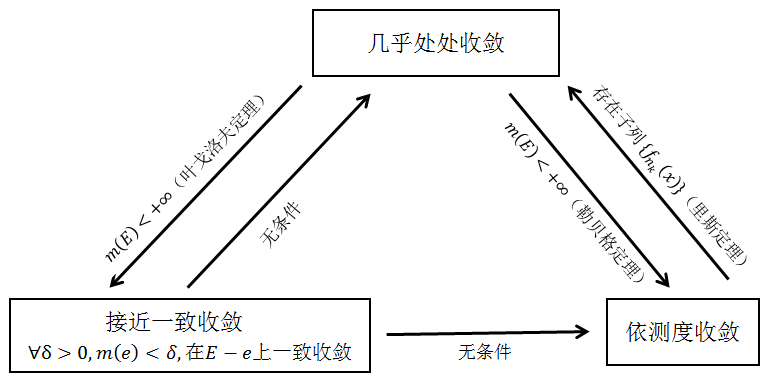
\includegraphics[width=0.8\textwidth]{image/Shoulianxing.png}
\caption{~几种收敛性间的关系} \label{fig33} 
\end{figure}

\section{可测函数与连续函数}

\subsection{卢津定理}

我们知道, 连续函数是可测函数, 可测函数可以由一列简单函数(互不相交闭集上的简单函数是连续函数)来逼近. 本节继续探讨可测函数与连续函数之间更进一步的联系.

\begin{lemma} \label{lem3.1}
设~$F_1,\,\cdots,\,F_n$~为~$\R^n$~中互不相交的闭集, 记~$F = \smallcup\limits_{k=1}^n F_k$, 则简单函数~$f(x) = \sum\limits_{k=1}^n c_k \chi_{F_k} (x)$~是~$F$~上的连续函数.
\end{lemma}

\begin{proof}
设~$x_0 \in F$, 则存在~$k_0$~使得~$x \in F_{k_0}$. 由于~$F_1,\,\cdots,\,F_n$~互不相交, 故~$x \notin \smallcup\limits_{k \neq k_0} F_k$. 又~$\smallcup\limits_{k \neq k_0} F_k$~闭, 则~$d\big(x_0,\,\smallcup\limits_{k \neq k_0} F_k\big) > 0$. 对~$\forall~\varepsilon > 0$, 记~$\delta = d\big(x_0,\,\smallcup\limits_{k \neq k_0} F_k\big)$. 则当~$x \in F$, 且~$d(x,\,x_0) < \delta$~时, 必有~$x \in F_{k_0}$. 从而
\[
|f(x) - f(x_0)| = |c_{k_0} - c_{k_0}| = 0 < \varepsilon
\]
因此, $f(x)$~在点~$x_0$~连续, 由~$x_0$~的任意性, $f(x)$~在~$F$~上连续.
\end{proof}

\begin{theorem}[卢津定理\index{卢津定理}]
设~$f(x)$~为可测集~$E$~上几乎处处有限的可测函数, 则对~$\forall~\delta > 0$, 存在闭集~$F \subset E$, 使得~$m(E - F) < \delta$, 且~$f(x)$~在~$F$~上连续.
\end{theorem}

\begin{proof}
由于~$m\big( \{x \in E: \: |f(x)| = +\infty\} \big) = 0$, 不妨设~$f(x)$~在~$E$~上处处有限.

(1) 若~$f(x)$~为简单函数, 即~$f(x) = \sum\limits_{k=1}^n c_k \chi_{E_k} (x)$, 其中~$E_1, \, \cdots, \, E_n$~可测互不相交且~$\mathop{\cup}\limits_{k=1}^n E_k = E$.

$E_k$~可测, 则对~$\forall~\delta > 0$, 存在闭集~$F_k \subset E_k$, 使得
\[
m(E_k - F_k) < \frac{\delta}{n}, \, \quad k = 1,\,\cdots,\,n
\]
令~$F = \mathop{\cup}\limits_{k=1}^n F_k$, 则~$F$~闭, $F \subset E$, 且
\begin{eqnarray*}
m(E - F) &=& m\big(\medcup\limits_{k=1}^n E_k - \medcup\limits_{k=1}^n F_k \big) = m\big( \medcup\limits_{k=1}^n (E_k - F_k) \big) \\
&\leqslant& \sum_{k=1}^n m(E_k - F_k) < \delta
\end{eqnarray*}
又~$f|_F(x) = \sum\limits_{k=1}^n c_k \chi_{F_k}(x)$, 由引理~\ref{lem3.1}~知~$f|_F$~连续.

(2) 若~$f(x)$~为有界可测函数, 由定理~\ref{thm312}, 存在简单函数列~$\{\varphi_n(x)\}$~在~$E$~上一致收敛于~$f(x)$.

由~(1), 对~$\forall~\delta > 0$~以及每个~$\varphi_n(x)$, 存在闭集~$F_n \subset E$~使得
\[
m(E - F_n) < \frac{\delta}{2^n}
\]
且~$\varphi_n(x)$~在~$F_n$~上连续. 令~$F = \mathop{\cap}\limits_{n=1}^\infty F_n$, 则~$F$~闭, $F \subset E$, 且
\begin{eqnarray*}
m(E - F) &=& m\big( E - \mathop{\cap}_{n=1}^\infty F_n \big) = m\big( \mathop{\cup}_{n=1}^\infty \big(E - F_n\big) \big) \\
&\leqslant& \sum_{n=1}^\infty m(E - F_n) < \sum_{n=1}^\infty \frac{\delta}{2^n} = \delta
\end{eqnarray*}
由于~$\varphi_n(x)$~在~$F$~上连续, 又
\[
\varphi_n(x) \rightrightarrows f(x), \, \quad x \in F \subset E
\]
故~$f(x)$~在~$F$~上连续(连续函数列的一致收敛极限是连续函数).

(3) 若~$f(x)$~为无界可测函数\footnote{可测函数有界与有限的区别: 有界必有限, 但有限不一定有界, 例如~$E=(0,\,1], \, f(x) = 1/x$~在~$E$~上每一点都有限, 但~$f(x)$~在~$E$~上无界.}, 做变换\footnote{``$\Rightarrow$''. $f(x) = g(x) \big( 1 + |f(x)|\big) = \frac{g(x)}{\frac{1}{1 + |f(x)|}} = \frac{g(x)}{1- \frac{|f(x)|}{1 + |f(x)|}} = \frac{g(x)}{1- |g(x)|}$; \\ ``$\Leftarrow$''. $g(x) = f(x)\big(1- |g(x)|\big) = \frac{f(x)}{\frac{1}{1- |g(x)|}} = \frac{f(x)}{1 + \frac{|g(x)|}{1- |g(x)|}} = \frac{f(x)}{1+ |f(x)|}$.}
\[
g(x) = \frac{f(x)}{1+ |f(x)|} \quad \Longleftrightarrow \quad f(x) = \frac{g(x)}{1- |g(x)|}
\]
则~$g(x)$~有界可测, 由~(2), 对~$\forall~\delta > 0$, 存在闭集~$F \subset E$~使得~$m(E - F) < \delta$, 且~$g|_F$~连续. 利用连续函数关于四则运算和~$|\cdot|$~运算封闭, $f(x)$~与~$g(x)$~的连续性
相同, 故~$f|_F$~连续.
\end{proof}

\begin{remark}
(i) 卢津定理说明, 可测函数可以在去掉任意小测度集~$E_\delta$~剩下的集合~$E - E_\delta$~上连续. 换句话说, 可测函数在某个小测度集上改变其函数值, 可以变成连续函数.

(ii) 卢津定理表明可测函数可由连续函数逼近(相差任意小的测度集的方式).

(iii) 定理条件~``~$m(E - F) < \delta$''~不能加强为~``~$m(E - F) = 0$''.
\end{remark}

\begin{example}
考虑狄利克雷函数
\[
D(x) = \left\{ \!\!
\begin{array}{ll}
1, & x \in \Q_{[0,1]} \\[0.1cm]
0, & x \in [0,\,1]-\Q_{[0,1]}
\end{array}
\right.
\]
记~$\Q_{[0,1]} = \{r_n\}_{n=1}^\infty$, 对~$\forall~\delta > 0$, 令
\[
F_\delta = [0,\,1] - \medcup_{n=1}^\infty \Big( r_n - \frac{\delta}{2^{n+1}},\, r_n + \frac{\delta}{2^{n+1}} \Big)
\]
则~$F_\delta$~闭, 且
\[
m\big([0,\,1] - F_\delta \big) = m \Big( \medcup_{n=1}^\infty \Big( r_n - \frac{\delta}{2^{n+1}},\, r_n + \frac{\delta}{2^{n+1}} \Big) \Big) \leqslant \sum_{n=1}^\infty \frac{\delta}{2^n} = \delta
\]
而~$D(x)$~在~$F_\delta$~上恒等于~$0$, 从而~$D(x)$~在~$F_\delta$~上是连续的.
\end{example}

\begin{theorem}[卢津定理的逆定理\index{卢津定理的逆定理}, 可测函数的又一定义]
设~$f(x)$~为可测集~$E$~上几乎处处有限的实值函数, 若对~$\forall~\delta > 0$, 存在闭集~$F_\delta \subset E$, 使得~$m(E - F_\delta) < \delta$, 且~$f(x)$~在~$F_\delta$~上连续, 则~$f(x)$~是~$E$~上的可测函数.
\end{theorem}

\begin{proof}
对每个~$n \in \N$, 都存在闭集~$F_n \subset E$~使得~$m(E - F_n) < 1/n$, 且~$f(x)$~在~$F_n$~上连续, 故~$f(x)$~在~$F_n$~上可测.

记~$F = \mathop{\cup}\limits_{n=1}^\infty F_n$, 则~$f(x)$~在~$F$~上可测. 由于~$F_n \subset F, \, n = 1,\,2,\,\cdots$, 故
\[
m(E - F) \leqslant m(E - F_n) < \frac{1}{n}, \, \quad n = 1,\,2,\,\cdots
\]
令~$n \to \infty$~得, $m(E - F) = 0$. 从而~$f(x)$~在~$E - F$~上可测. 因此, $f(x)$~在~$E = F \cup (E - F)$~上可测.
\end{proof}

\begin{theorem}[卢津定理的另一种形式\index{卢津定理的另一种形式}] \label{thm333}
设~$f(x)$~为可测集~$E$~上几乎处处有限的可测函数, 则对~$\forall~\delta > 0$, 都存在~$\R^n$~上的连续函数~$g(x)$~使得
\[
m\big(\{x \in E: \: f(x) \neq g(x)\} \big) < \delta
\]
且~$\sup\limits_{x \in \R^n} |g(x)| \leqslant \sup\limits_{x \in E} |f(x)|$. 若~$E$~是有界集, 则可要求~$g(x)$~具有紧支集\footnote{集合~$\{x \in D(f): \: f(x) \neq 0\}$~称为函数~$f$~的支撑集, 记为~$\mathrm{supp~}\!(f)$. 若~$\mathrm{supp~}\!(f)$~是紧集, 则称函数~$f$~具有紧支集. }.
\end{theorem}

\begin{proof}
由卢津定理, 对~$\forall~\delta > 0$, 存在闭集~$F \subset E$~使得~$m(E - F) < \delta$, 且~$f(x)$~在~$F$~上连续. 由连续函数延拓定理~\ref{thm1414}, 存在~$\R^n$~上的连续函数~$g(x)$~使得
\[
g(x) = f(x), \, \quad x \in F
\]
且~$\sup\limits_{x \in \R^n} |g(x)| \leqslant \sup\limits_{x \in E} |f(x)|$.
由于
\[
\{x \in E: \: f(x) \neq g(x)\} \subset E - F
\]
故
\[
m\big(\{x \in E: \: f(x) \neq g(x)\} \big) \leqslant m(E - F) < \delta
\]

若~$E$~有界, 不妨设~$E \subset B(0,\,r)$. 作~$\R^n$~上的连续函数~$\varphi(x)$, 满足~$0 \leqslant \varphi(x) \leqslant 1$, 且
\[
\varphi(x) = \left\{\!\!
\begin{array}{ll}
1, & x \in E \\[0.1cm]
0, & x \notin B(0,\,r)
\end{array}
\right.
\]
则把~$g(x)$~换成~$\varphi(x)g(x)$~即为所求.
\end{proof}

\begin{theorem}
设~$f(x)$~为可测集~$E$~上几乎处处有限的可测函数, 则存在~$E$~上的连续函数列~$\{f_n(x)\}$~
使得~$f_n \xrightarrow{\mathrm{a.e.}} f$.
\end{theorem}

\begin{proof}
由定理~\ref{thm333}, 对每个~$n \in \N$, 都存在~$\R^n$~上的连续函数~$g_n(x)$~满足
\[
m\big(\{x \in E: \: f(x) \neq g_n(x)\} \big) < \frac{1}{n}
\]
从而, 对~$\forall~\varepsilon > 0$
\begin{eqnarray*}
&& m\big( \{x \in E: \: |g_n(x) - f(x)| \geqslant \varepsilon \} \big) \\
&\leqslant& m\big(\{x \in E: \: f(x) \neq g_n(x)\} \big) < \frac{1}{n} \longrightarrow 0
\end{eqnarray*}
当~$n \to \infty$~时. 故~$g_n \xrightarrow{~\mu~} f$. 由里斯定理, 存在~$\{g_n\}$~的子列~$\{g_{n_k}\}$~
使得~$g_{n_k} \xrightarrow{\mathrm{a.e.}} f$. 再取~$f_k = g_{n_k}|_E$~即可.
\end{proof}

\section{测度论与概率论的关系$^\ast$}

测度论是概率论的理论基础, 所以, 概率论中的一些概念抽象化就是对应的测度论中的概念. 

概率是要度量``事件发生的可能性''的大小, 事件的抽象化描述就是集合, 需要考察``事件的全体'', 对应到测度论就是``集合系''. ``事件发生的可能性''是对事件的一种度量, 对应到测度论就是``集合的测度''. 

不是每个事件都可以定义其概率（发生的可能性的大小）的, 对应的就是不是每个集合都可以定义测度, 可以定义测度集合就是可测集. 同时, 事件必然要涉及到事件的组合运算（复杂事件是可由基本事件表示出来）, 对应的就是集合的交、并、差、余、极限的运算到复杂集合, 所以又需要保证做可列次这些运算不能超出全体范围（即可测集的范围要足够大, 以保证集合的可列次交、并、差、余、极限等的运算之后还在里面）.

那么什么样的集合系, 才能保证其中的集合是可测集（可以定义测度，又对那些运算封闭）呢? 测度论中讲了, 只要集合系是~$\sigma$-代数就可以了。$\sigma$-代数的基本定义是: 

\begin{publist}
	\item[(1)] 全集在里面; 
	
	\item[(2)] 里面每个集合的余集在里面; 
	
	\item[(3)] 里面任意可列个集合的并集在里面.
\end{publist}

\noindent 有了这三条基本定义, 就可以推出: 空集、可列次交、并、差、上限集、下限集等运算之后都能在里面, 就满足需要了.

所以, 集合~$X$, 再加上该集合上的一个~$\sigma$-代数~$\F$, $(X, \F)$~就是一个可测空间了, 即可以定义测度的空间, $\F$~中任一集合都可以定义其测度（集合大小的某种度量）. 进一步再定义了测度~$\mu$, 那么~$(X,\F,\mu)$~就是测度空间.

对应到概率论中, 样本空间（集合）~$\Omega$, 事件域~$\F$（$\sigma$-代数），概率测度~$P$（测度）, 放一起~$(\Omega,\F,P)$~就是概率测度空间, 简称概率空间. 概率测度~$P$~是满足特殊要求的一种测度: $P(\Omega)=1$.

Borel~$\sigma$-代数~$\mathfrak{B}_\R$, 表示实数轴~$\R$~上的~$\sigma$-代数, 可由实轴上的所有开集生成, 也可由实数轴上所有的~$(-\infty,a]$~这样的区间生成, 是相等的. 按~$\sigma$-代数定义, 实数轴上开集、闭集的至多可列次交、并、差（余）、上限集、下限集、极限集的运算, 都超不出该~Borel~$\sigma$-代数的范围.

$\mathfrak{B}_\R$~有什么用? 其实概率论中的随机变量, 对应测度论中的可测函数, 而可测函数就是从可测空间~$(X,\F)$~到~$(\R, \mathfrak{B}_\R)$~的可测映射: 即~$\mathfrak{B}_\R$~中的任一集合在该映射下的原像都属于~$\F$（即都是~$X$~上的可测集）.

再说说随机变量, 前面说了概率论中要用集合表示事件, 但事件五花八门, 怎么统一用一种简单的集合表示呢? 这就用到映射的概念, 建立一种从样本空间（基本事件的全体）到实数轴的映射（一一对应）就可以了, 这种映射就是随机变量. 有了它，基本事件映射到实数轴上就是的基本区间, 基本事件经过运算生成的复杂事件, 映射到实数轴上就是~$\mathfrak{B}_\R$中的集合, 即~Borel~集. 

因为有了这个对应关系, 要度量``事件发生的可能性的大小''（即概率测度）, 只要度量``实数轴上~Borel~$\sigma$-代数中的集合'' 就可以了. 而~$\mathfrak{B}_\R$~是~$\sigma$-代数是可以定义测度的, 于是给~$\mathfrak{B}_\R$~中的集合定义概率测度就行了.

所以, 随机变量的测度论语言定义是这样的: 设~$(\Omega,\F,P)$~为概率空间，若对实数轴上~$\sigma$-代数~$\mathfrak{B}_\R$~中的任一集合~$B$, 都有~$\{ \omega \in \Omega: X(\omega) \in B\} \in \F$, 则称~$X(\omega)$~为随机变量, 也简记为~$X$.

总之, 随机变量就是建立了``随机事件''到``实数轴上~Borel~$\sigma$-代数''的一种对应, 并且保证了建立了这种对应的随机事件都是可以定义概率测度的. 

既然随机事件~$\{\omega \in \Omega: X(\omega) \in B\}$~属于~$\F$, 那么可以有概率, 即~$P\{\omega \in \Omega: X(\omega) \in B\}$~是有意义的. 为了简单, 概率中简记
\[
P\{\omega \in \Omega: X(\omega) \in B\} = P\{X \in B\}
\] 

特别地, 若取~$B=(-\infty,x)$, 则事件~$\{X \in B\}$~的概率
\[
P\{X \in B\} = P\{X \leqslant x\} := F(x)
\]
就定义成随机变量~$X$~的分布函数. 因为对任意的区间~$(a,b]$, 都可表示成
\[
P\{X \in (a,b] \} = P\{a < X \leqslant b\} = P\{X \leqslant b\} - P\{X \leqslant a\} = F(b)-F(a)
\]
进而, 由这样的区间经过至多可列次交、并、差运算的复杂的实数轴上的~Borel~集都可以用~$F(x)$~给出其概率.

当然, 随机变量也可以定义为从样本空间到平面~$\R^2$~上的映射, 就是二元随机变量.

\newpage
\begin{problemset}

\item $f$~可测~$\Leftrightarrow$~对~$\forall~r \in \Q$, $\{x \in E: \: f(x) > r\}$~是可测集. 若~``~$f(x) > r$~''~换成~``~$f(x) = r$~'', 结论不成立.

\item 设~$f(x)$~是~$E$~上的可测函数, $G,\,F$~分别为~$\R$~中的开集和闭集, 问
    \[
    \{x \in E: \: f(x) \in G\}, \quad \{x \in E: \: f(x) \in F\}
    \]
    是否是可测集? 下列结论是否成立?

\begin{enumerate}
  \item[(1)] $f$~可测~$\Leftrightarrow$~对任意的开集~$G \subset \R$, $\{x \in E: \: f(x) \in G\}$~是可测集.
  \item[(2)] $f$~可测~$\Leftrightarrow$~对任意的闭集~$F \subset \R$, $\{x \in E: \: f(x) \in F\}$~是可测集.
\end{enumerate}

\item 从函数~$f^2(x)$~或~$|f(x)|$~可测, 能否推出~$f(x)$~也可测?

\item 由~$f(x)\pm g(x)$~可测, 能否推出~$f(x),\,g(x)$~都可测?

\item 设~$\{f_n(x)\}$~为~$E$~上的可测函数列, 能否断定~$\sum\limits_{n=1}^\infty f_n(x)$~为~$E$~上的可测函数?

\item 设~$E$~是~$[0,\,1]$~中的不可测集
\[
f(x) = \left\{\!\!
\begin{array}{cl}
x, \, & x \in E \\[0.1cm]
-x, \, & x \in [0,\,1] - E
\end{array}
\right.
\]
问~$f(x)$~在~$[0,\,1]$~上是否可测? $|f(x)|$~是否可测?

\item 设~$\{f_n(x)\}$~为~$E$~上的可测函数列, 则其收敛点集与发散点集都是可测的.

\item 试证如下的黎曼函数是可测函数
\[
R(x) = \left\{\!\!
\begin{array}{cl}
\dfrac{1}{n}, \, &  x = \dfrac{m}{n} \\[0.2cm]
0, \, &  x \mbox{~为无理数}
\end{array}
\right.
\]
(其中, $x \in [0,\,1],\,m,\,n$~互质, 且~$m \leqslant n$).

\item 设~$f(x)$~为~$E$~上几乎处处有限的可测函数, $m(E) < +\infty$, 则对~$\forall~\varepsilon > 0$, 都存在有界可测函数~$g(x)$~使得
\[
m\big( \{x \in E:\: f(x) \neq g(x) \}\big) < \varepsilon
\]

\item 设~$f(x)$~为~$E$~上的可测函数, $g(x)$~为~$\R$~上的波雷尔可测函数, 试证 $g(f)$~是~$E$~上的可测函数.

\item 设~$f(x)$~为~$[a,\,b]$~上的可微函数, 则~$f'(x)$~在~$[a,\,b]$~上可测.

\item 设在可测集~$E$~上有~$f_n \xrightarrow{\mathrm{a.e.}} f, \, g_n \xrightarrow{\mathrm{a.e.}} g$. 证明:

\begin{enumerate}
  \item[(1)] $a f_n + b g_n \xrightarrow{\mathrm{a.e.}} a f + b g, \, \forall~a,\,b \in \R$;
  \item[(2)] $|f_n| \xrightarrow{\mathrm{a.e.}} |f|$;
  \item[(3)] $\sup\{f_n,\,g_n\} \xrightarrow{\mathrm{a.e.}} \sup\{f,\,g\}$; $\inf\{f_n,\,g_n\} \xrightarrow{\mathrm{a.e.}} \inf\{f,\,g\}$.
\end{enumerate}

\item 设在可测集~$E$~上有~$f_n \xrightarrow{~\mu~} f, \, g_n \xrightarrow{~\mu~} g$. 证明:

\begin{enumerate}
  \item[(1)] $a f_n + b g_n \xrightarrow{~\mu~} a f + b g, \, \forall~a,\,b \in \R$;
  \item[(2)] $|f_n| \xrightarrow{~\mu~} |f|$;
  \item[(3)] $\sup\{f_n,\,g_n\} \xrightarrow{~\mu~} \sup\{f,\,g\}$; $\inf\{f_n,\,g_n\} \xrightarrow{~\mu~} \inf\{f,\,g\}$.
\end{enumerate}

\item 设~$m(E) > 0$, $\{f_n(x)\}$~为~$E$~上几乎处处有限的可测函数列, 且~$f_n \xrightarrow{\mathrm{a.e.}} f$, 则存在常数~$C$~与~$E_0 \subset E$, 满足~$m(E_0) > 0$, 且
    \[
    |f_n(x)| \leqslant C, \, \quad \forall~x \in E_0, \, n \in \N
    \]

\item 设~$m(E) < +\infty$, 对于在~$E$~中每点都趋于~$+\infty$~的函数列建立叶戈洛夫定理.

\item 问当~$m(E)=+\infty$~时, 卢津定理是否仍然成立?

\item 试作~$E = [0,\,1]$~上的可测函数~$f(x)$, 使得对~$E$~上任意连续函数~$g(x)$~都有
    \[
    m\big(\{x \in E: \: f(x) \neq g(x)\} \big) \neq 0
    \]
    此结果与卢津定理有无矛盾?

\item 设对每个给定的~$n$, 当~$k \to \infty$~时, $f_k^{(n)}(x) \xrightarrow{~\mu~} f^{(n)}(x)$, 且当~$n \to \infty$~时, $f^{(n)}(x) \xrightarrow{~\mu~} f(x)$. 则在~$\big\{ f_k^{(n)}(x) \big\}$~中可以选取函数列依测度收敛于~$f(x)$.

\item 设~$f_n \xrightarrow{~\mu~} f$, 且对每个~$n \in \N$~都有~$f_n(x) \leqslant g(x)$. 证明~$f(x) \leqslant g(x), \, \mathrm{~a.e.~} x \in E$.

\item 设~$f_n \xrightarrow{~\mu~} f$, 且对每个~$n \in \N$~都有~$f_n(x) \leqslant f_{n+1}(x), \, \mathrm{~a.e.~} x \in E$. 证明~$f_n \xrightarrow{\mathrm{a.e.}} f$.

\item 设~$f(x),\,f_1(x),\,\cdots,\, f_k(x),\,\cdots$~为~$E=[a,\,b]$~上几乎处处有限的可测函数, 且在~$E$~上有~$f_k \xrightarrow{\mathrm{a.e.}} f$. 则存在可测集~$E_n \subset [a,\,b]$, $n=1,\,2,\,\cdots$, 使得
    \[
    m\Big( [a,\,b]-\medcup_{n=1}^\infty E_n \Big) = 0
    \]
    而在每个~$E_n$~上有~$f_k \rightrightarrows f$.

\item 设~$f(x)$~为~$[a,\,b]$~上的几乎处处有限的可测函数, 则对任意的~$\varepsilon > 0$~及~$\delta > 0$, 都存在闭集~$F \subset [a,\,b]$~及多项式函数~$P(x)$, 使得~$m(F) > b-a-\delta$, 且
    \[
    \big| f(x) - P(x) \big| < \varepsilon, \quad x \in F
    \]

\item 设~$f(x)$~为~$[a,\,b]$~上的实值可测函数, 证明: 存在数列~$\{h_n\}$, 使得
    \[
    \lim_{n \to \infty} h_n = 0, \, \quad \lim_{n \to \infty} f(x+h_n) = f(x), \quad \mathrm{~a.e.~} x \in [a,\,b]
    \]

\item 设~$\{f_n(x)\}$~为~$[0,\,1]$~上几乎处处收敛于~$0$~的可测函数列, 证明: 存在数列~$\{t_n\}$, 使得
\[
\sum_{n=1}^\infty |t_n| = +\infty, \, \quad \sum_{n=1}^\infty \big| t_n f_n(x) \big| < +\infty, \quad \mathrm{~a.e.~} x \in [0,\, 1]
\]
\end{problemset}



\chapter{勒贝格积分}

前言中介绍了黎曼积分存在的某些缺陷, 这些缺陷限制了黎曼积分的应用. 二十世纪初,
法国数学家勒贝格~(1875--1941)~创建了一种新的勒贝格积分理论.

勒贝格积分是在勒贝格测度理论的基础上建立起来的, 这一理论可以统一处理函数有界和无界的情形. 黎曼积分通常讨论的是闭区间~$[a,\, b]$~上的函数, 而勒贝格积分定义域可以是更一般的点集即可测集. 更重要的是, 它提供了比黎曼积分更广泛而有用的收敛定理.

本章先由简单函数的勒贝格积分入手, 然后到非负可测函数, 再到一般可测函数的勒贝格积分; 并讨论了勒贝格积分的性质, 特别是列维定理, 法都引理与勒贝格控制收敛定理; 另外, 进一步发掘黎曼积分和勒贝格积分内在联系, 并给出黎曼可积函数的一个判别条件.

\section{勒贝格积分的定义}

\subsection{非负简单函数的勒贝格积分}

\begin{definition}
设~$f(x)$~为~$E$~上的非负简单函数, 记~$f(x) = \sum\limits_{i=1}^n a_i \chi_{E_i}(x)$,  其中~$E_i$~可测、互不相交, 且~$\smallcup\limits_{i=1}^n E_i = E$, 定义
\[
(L)\int_E f(x) \d \mu = \sum_{i=1}^n a_i m(E_i)
\]
称为~$f(x)$~在~$E$~上(关于测度~$m$~)的勒贝格积分.
\end{definition}

\begin{remark}
(1) $\int_E f(x) \d \mu$~可以是~$+\infty$.

\vspace{0.5ex}

(2) $\int_E f(x) \d \mu = \int_{\mathbb{R}^n} f(x) \chi_E (x) \d \mu$.

\vspace{0.5ex}

(3) 数值~$\int_E f(x) \d \mu$~是确定的, 即不依赖于~$f$~表达式的选取.
\end{remark}


\begin{lemma} \label{lem410}
设~$f(x)=\sum\limits_{i=1}^n a_i \chi_{E_i}(x)$, $g(x)=\sum\limits_{j=1}^m b_j \chi_{e_j}(x)$~为~$E$~上的简单函数，则它们可以表示为统一形式：
\[
f(x)=\sum\limits_{i=1}^n \sum\limits_{j=1}^m a_i \chi_{E_i \cap e_j}(x), \qquad g(x)= \sum\limits_{i=1}^n \sum\limits_{j=1}^m b_j \chi_{E_i \cap e_j}(x)
\]
实际上，对于~$E$~的两种划分：$E=\mathop{\smallcup}\limits_{i=1}^n E_i=\mathop{\smallcup}\limits_{j=1}^m e_j$, 其中，$E_i$~互不相交，$e_j$~互不相交。则
\[
E=\mathop{\smallcup}\limits_{i=1}^n E_i = \mathop{\smallcup}\limits_{i=1}^n (E_i \cap E) = \mathop{\smallcup}\limits_{i=1}^n \Big(E_i \cap \mathop{\smallcup}\limits_{j=1}^m e_j \Big) =\mathop{\smallcup}\limits_{i=1}^n \mathop{\smallcup}\limits_{j=1}^m (E_i \cap e_j)
\]
显然，$(E_i \cap e_j)$~互不相交，且包含于~$E_i$~和~$e_j$, 故结论成立。
\end{lemma}

\begin{proof}
设~$f(x) = \sum\limits_{j=1}^m b_j \chi_{e_j}(x)$~为~$f$~的又一表达式, 则由引理~\ref{lem410}~知
\[
f(x)=\sum\limits_{i=1}^n \sum\limits_{j=1}^m a_i \chi_{E_i \cap e_j}(x) = \sum\limits_{i=1}^n \sum\limits_{j=1}^m b_j \chi_{E_i \cap e_j}(x)
\]
注意到，在~$(E_i \cap e_j)$~上有~$a_i=b_j$, 从而
\[
\int_E f(x) \d \mu = \sum_{i=1}^n \sum_{j=1}^m a_i m(E_i \cap e_j) = \sum_{i=1}^n \sum_{j=1}^m b_j m(E_i \cap e_j)
\]
因此, 非负简单函数勒贝格积分的定义有意义.
\end{proof}

\begin{example}
狄利克雷函数
\[
D(x) = \left\{ \!\!
\begin{array}{ll}
1,\, & x \mbox{~为~} [0,\, 1] \mbox{~上的有理数~} \\[0.1cm]
0,\, & x \mbox{~为~} [0,\, 1] \mbox{~上的无理数~}
\end{array}
\right.
\]
则~$D(x)$~的勒贝格积分
\[
(L)\int_{[0,1]} D(x) \d \mu = 1 \cdot m\big(\mathbb{Q}_{[0,1]}\big) + 0 \cdot m\big([0,\, 1] - \mathbb{Q}_{[0,1]} \big) = 0
\]
\end{example}

\begin{example}
设~$E \subset \mathbb{R}^n$~可测, 则
\[
\int_E 1 \d \mu = \int_{\mathbb{R}^n} \chi_E(x) \d \mu = m(E)
\]
\end{example}

\begin{proposition} \label{prop411}
设~$f(x),\,g(x)$~为~$E$~上的非负简单函数, 则

(i) $\int_E c f(x) \d \mu = c \int_E f(x) \d \mu, \, c \geqslant 0$~为实数;

(ii) $\int_E \big[f(x) + g(x)\big] \d \mu = \int_E f(x) \d \mu + \int_E g(x) \d \mu$;

(iii) 若~$f(x) \leqslant g(x),\, \mathrm{~a.e.~} x \in E$, 则~$\int_E f(x) \d \mu \leqslant \int_E g(x) \d \mu$.
\end{proposition}

\begin{proof}
(i) 显然成立.

(ii) 设~$f(x) = \sum\limits_{i=1}^n a_i \chi_{A_i}(x),\,g(x) = \sum\limits_{j=1}^m b_i \chi_{B_j}(x)$, 则由引理~\ref{lem410}~知
\[
f(x) = \sum\limits_{i=1}^n \sum\limits_{j=1}^m a_i \chi_{A_i \smallcap B_j} (x), \qquad g(x) = \sum\limits_{i=1}^n \sum\limits_{j=1}^m b_j \chi_{A_i \smallcap B_j} (x)
\]
从而
\[
f(x) + g(x) = \sum\limits_{i=1}^n \sum\limits_{j=1}^m (a_i + b_j) \chi_{A_i \smallcap B_j} (x)
\]
于是
\begin{eqnarray*}
\int_E [f(x)+g(x)] \d \mu &=& \sum_{i=1}^n \sum_{j=1}^m (a_i + b_j) m(A_i \medcap B_j) \\
&=& \sum_{i=1}^n \sum_{j=1}^m a_i m(A_i \medcap B_j) + \sum_{i=1}^n \sum_{j=1}^m b_j m(A_i \medcap B_j) \\
&=& \int_E f(x) \d \mu + \int_E g(x) \d \mu
\end{eqnarray*}

(iii) 由引理~\ref{lem410}, 不妨设~$f(x) = \sum\limits_{i=1}^n a_i \chi_{A_i}(x),\, g(x) = \sum\limits_{i=1}^n b_i \chi_{A_i}(x)$, 其中, $E = \mathop{\smallcup}\limits_{i=1}^n A_i$. 由于~$f(x) \leqslant g(x),\, \mathrm{~a.e.~} x \in E$, 则存在~$e \subset E,\, m(e) = 0$, 使得
\[
f(x) \leqslant g(x),\quad  \forall~x \in E - e
\]
由于
\[
A_i = A_i \medcap E = A_i \medcap \big((E-e) \medcup e\big) = \big(A_i \medcap (E-e)\big) \medcup (A_i \medcap e)
\]
故
\[
f(x) = \sum_{i=1}^n \big[ a_i \chi_{A_i \cap (E-e)}(x) + a_i \chi_{A_i \cap e}(x) \big]
\]
注意到~$m(A_i \smallcap e) = 0$, 从而
\begin{eqnarray*}
\int_E f(x) \d \mu &=& \sum_{i=1}^n \big[ a_i m\big(A_i \medcap (E-e)\big) + a_i m(A_i \medcap e) \big] \\
&\leqslant& \sum_{i=1}^n b_i m\big(A_i \medcap (E-e)\big) \\
&=& \sum_{i=1}^n \big[ b_i m\big(A_i \medcap (E-e)\big) + b_i m(A_i \medcap e) \big] \\
&=& \int_E g(x) \d \mu
\end{eqnarray*}
\end{proof}

\subsection{非负可测函数的勒贝格积分}

\begin{definition}
设~$f(x)$~为~$E$~上的非负可测函数, 定义
\[
(L)\int_E f(x) \d \mu = \sup \Big\{ \int_E \varphi(x) \d \mu: \: \varphi \mbox{~为~} E \mbox{~上简单函数且~} 0 \leqslant \varphi \leqslant f \Big\}
\]
称为~$f(x)$~在~$E$~上的勒贝格积分.
\end{definition}

\begin{theorem} \label{thm411}
设~$f(x)$~为~$E$~上的非负可测函数, 则存在单调递增的非负简单函数列~$\{f_n(x)\}$~使得
\[
\int_E f(x) \d \mu = \lim_{n \to \infty} \int_E f_n(x) \d \mu
\]
\end{theorem}

\begin{proof}
$f(x)$~在~$E$~上非负可测, 由可测函数构造定理, 存在单调递增的非负简单函数列~$\{f_n(x)\}$~使得
\[
f(x) = \lim\limits_{n \to \infty} f_n(x),\, \quad x \in E
\]
只需证明
\[
\lim_{n \to \infty} \int_E f_n(x) \d \mu = \sup \Big\{ \int_E \varphi(x) \d \mu: \: \varphi \mbox{~为~} E \mbox{~上简单函数且~} 0 \leqslant \varphi \leqslant f \Big\}
\]
显然, 左端~$\leqslant$~右端.

反过来, 设~$\varphi(x)$~为~$E$~上的非负简单函数, 且~$\varphi(x) \leqslant f(x),\, x \in E$. 由于~$\{f_n(x)\}$~单调递增, 由命题~\ref{prop411}~(iii), $\int_E f_n(x) \d \mu$~也单调递增, 故~$\lim\limits_{n \to \infty} \int_E f_n(x) \d \mu$~存在(或~$= +\infty$).

记~$\varphi(x) = \sum\limits_{i=1}^m a_i \chi_{E_i}(x)$, 其中~$\mathop{\smallcup}\limits_{i=1}^m E_i = E$. 对~$\forall~\varepsilon > 0$(不妨设~$\varepsilon < 1$), 对每个~$i = 1, \, \cdots, \, m$, 以及~$n \in \mathbb{N}$, 令
\[
E_{i,n}=\big\{x \in E_i: \: f_n(x) \geqslant (1- \varepsilon) a_i \big\}
\]
则由~$\{f_n(x)\}$~可测且单调递增知, $\big\{E_{i,n} \big\}_{n=1}^\infty$~是单调递增的可测集列. 下面证明~$E_i = \mathop{\smallcup}\limits_{n=1}^\infty E_{i,n}$.

显然有~$\mathop{\smallcup}\limits_{n=1}^\infty E_{i,n} \subset E_i$. 对~$\forall~x \in E_i$,   则~$\varphi(x) = a_i$. 由于
\[
\lim_{n \to \infty} f_n(x) = f(x) \geqslant \varphi(x)
\]
则对上述~$\varepsilon$, 存在~$n_0 \in \mathbb{N}$~使得
\[
f_{n_0}(x) > (1 - \varepsilon) f(x) \geqslant (1- \varepsilon) \varphi(x) = (1- \varepsilon) a_i
\]
故
\[
x \in E_{i,n_0} \subset \mathop{\medcup}\limits_{n=1}^\infty E_{i,n}
\]
从而
\[
E_i \subset \mathop{\medcup}\limits_{n=1}^\infty E_{i,n}
\]
因此, $E_i = \mathop{\smallcup}\limits_{n=1}^\infty E_{i,n}$.

\vspace{0.2cm}

对每个~$n \in \mathbb{N}$, 令
\[
\varphi_n(x) = \sum_{i=1}^m (1- \varepsilon) a_i \chi_{E_{i,n}}(x),\, \quad x \in E
\]
则~$\{\varphi_n(x)\}$~为~$E$~上的非负简单函数列, 且满足~$f_n(x) \geqslant \varphi_n(x),\,  \forall~n \in \mathbb{N}$. 注意到~$\big\{E_{i,n} \big\}_{n=1}^\infty$~单调递增, 利用单调可测集列测度的极限性质
\begin{eqnarray*}
\lim_{n \to \infty} \int_E f_n(x) \d \mu &\geqslant& \lim_{n \to \infty} \int_E \varphi_n(x) \d \mu = \lim_{n \to \infty} \sum_{i=1}^m (1- \varepsilon) a_i m(E_{i,n}) \\
&=& \sum_{i=1}^m (1- \varepsilon) a_i \lim_{n \to \infty} m(E_{i,n}) \\
&=& \sum_{i=1}^m (1- \varepsilon) a_i m\Big( \medcup_{n=1}^\infty E_{i,n} \Big) \\
&=& \sum_{i=1}^m (1- \varepsilon) a_i m(E_i)
\end{eqnarray*}
令~$\varepsilon \to 0$~得
\[
\lim\limits_{n \to \infty} \int_E f_n(x) \d \mu \geqslant \sum_{i=1}^m a_i m(E_i) = \int_E \varphi(x) \d \mu
\]
再由~$\varphi(x)$~的任意性, 对所有这样的~$\varphi$~取~$\sup$~可得左端~$\geqslant$~右端.
\end{proof}

\begin{remark} \label{rem411}
该定理表明对于非负递增简单函数列, 积分号与极限号是可交换的, 即
\[
\int_E \lim_{n \to \infty} f_n(x) \d \mu = \lim_{n \to \infty} \int_E f_n(x) \d \mu
\]
\end{remark}

\begin{proposition} \label{prop412}
设~$f(x),\, g(x)$~为~$E$~上的非负可测函数, 则

(i) $\int_E c f(x) \d \mu = c \int_E f(x) \d \mu, \, c \geqslant 0$~为实数;

(ii) $\int_E \big[f(x) + g(x)\big] \d \mu = \int_E f(x) \d \mu + \int_E g(x) \d \mu$;

(iii) 若~$f(x) \leqslant g(x),\,  \mathrm{~a.e.~} x \in E$, 则~$\int_E f(x) \d \mu \leqslant \int_E g(x) \d \mu$.
\end{proposition}

\begin{proof}
由定理~\ref{thm411}, 命题~\ref{prop411}, 及极限性质易知~(i), (ii)~成立.

(iii) 取非负简单函数列~$\{f_n\} \nearrow f,\,  \{g_n\} \nearrow g$. 由于~$f(x) \leqslant g(x),\,  \mathrm{~a.e.~} x \in E$, 则可以适当选取~$f_n(x) \leqslant g_n(x),\,   \mathrm{~a.e.~} x \in E$. 由命题~\ref{prop411}~(iii)
\[
\int_E f(x) \d \mu = \lim_{n \to \infty} \int_E f_n(x) \d \mu \leqslant \lim_{n \to \infty}\int_E g_n(x) \d \mu = \int_E g(x) \d \mu
\]
故结论成立.
\end{proof}

\subsection{一般可测函数的勒贝格积分}

\begin{definition}
设~$f(x)$~为~$E$~上的可测函数, 记~$f(x) = f^+(x) - f^-(x)$, 其中，$f^+, \, f^-$~分别为~$f$~的正部和负部，若~$\int_E f^+(x) \d \mu$~与~$\int_E f^-(x) \d \mu$~至少有一个有限, 则定义
\[
(L) \int_E f(x) \d \mu = \int_E f^+(x) \d \mu - \int_E f^-(x) \d \mu
\]
称为~$f(x)$~在~$E$~上的勒贝格积分\index{勒贝格积分}, 也简称~$f(x)$~在~$E$~上的~L-积分存在.

若~$\int_E f(x) \d \mu$~有限, 或等价地
\[
\int_E f^+(x) \d \mu < +\infty \quad \mbox{~且~} \quad \int_E f^-(x) \d \mu < +\infty
\]
则称~$f(x)$~在~$E$~上是勒贝格可积\index{勒贝格可积}的, 简称~L-可积. 可测集~$E$~上勒贝格可积函数的
全体, 记为~$L(E)$.
\end{definition}

下面看勒贝格积分的几何意义, 考察一维可测点集~$E$~上的~L-可积函数~$f(x)$. 记
\[
G(f^+) = \{(x,\, y): \: x \in E, \,  0 \leqslant y \leqslant f^+(x) \}
\] \[
G(f^-) = \{(x,\, y): \: x \in E, \, 0 \leqslant y \leqslant f^-(x) \}
\]
则~$\int_E f(x) \d \mu$~的几何意义就是二维点集~``$G(f^+)$~的面积''~减去~``$G(f^-)$~的面积'', 即
\[
\int_E f(x) \d \mu = m\big( G(f^+) \big) - m\big( G(f^-) \big)
\]
这与黎曼积分的情形类似. 同理, 对于~$E \subset \mathbb{R}^n$, $G(f^+),\,  G(f^-)$~就是~$n+1$~维点集, 则~$m\big( G(f^+) \big),\, m\big( G(f^-) \big)$~表现为~$\mathbb{R}^{n+1}$~上的测度. 更一般地,

\begin{definition}
设~$f(x)$~为~$E \subset \R^n$~上的非负可测函数, 则称如下的~$n+1$~维点集
\[
G(E,\, f):=\big\{ (x,\, y): \: x \in E,\, 0 \leqslant y \leqslant f(x) \big\}
\]
为函数~$f$~的下方图形\index{下方图形}.
\end{definition}

\begin{figure}[!htb]
\centering
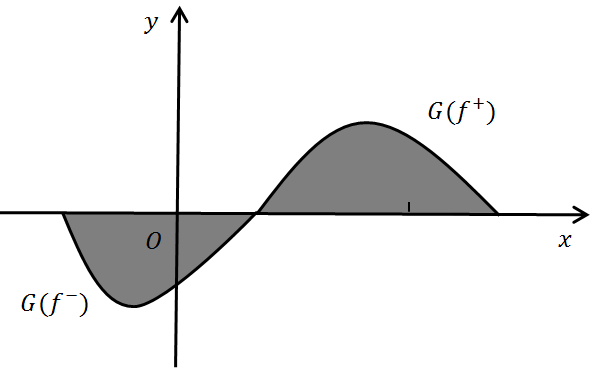
\includegraphics[width=0.6\textwidth]{image/Ljifenjiheyiyi.png}
\vspace*{-0.2cm}
\caption{~L-积分的几何意义} \label{fig41} 
\end{figure}


\section{勒贝格积分的性质}

\subsection{L-积分的基本性质}

\begin{proposition} \label{prop413}
设~$f(x),\, g(x)$~在~$E$~上的~L-积分存在, 则

(i) 对~$\forall~c \in \mathbb{R}$, $c f(x)$~的~L-积分存在, 且~$\int_E c f(x) \d \mu = c \int_E f(x) \d \mu$;

(ii) 若~$\int_E f(x) \d \mu + \int_E g(x) \d \mu$~有意义, 则~$f(x) + g(x)$~的~L-积分存在, 且
\[
\int_E \big[f(x) + g(x)\big] \d \mu = \int_E f(x) \d \mu + \int_E g(x) \d \mu
\]

(iii) 若~$f(x) \leqslant g(x),\,  \mathrm{~a.e.~} x \in E$, 则~$\int_E f(x) \d \mu \leqslant \int_E g(x) \d \mu$.
\end{proposition}

\begin{proof}
(i) 若~$c \geqslant 0$, 则~$(cf)^+ = c f^+,\, (cf)^- = c f^-$. 由~$f$~的~L-积分存在易知~$cf$~的~L-积分也存在. 再由命题~\ref{prop412}
\begin{eqnarray*}
\int_E cf(x) \d \mu &=& \int_E (cf)^+(x) \d \mu - \int_E (cf)^-(x) \d \mu \\
&=& \int_E c f^+(x) \d \mu - \int_E c f^-(x) \d \mu \\
&=& c \int_E f(x) \d \mu
\end{eqnarray*}
若~$c < 0$, 则~$(cf)^+ = -c f^-, \, (cf)^- = -c f^+$. 类似可证结论成立.

(ii) 由于~$(f+g)^+ - (f+g)^- = f + g = f^+ - f^- + g^+ - g^-$, 故
\[
(f+g)^+ + f^- + g^- = (f+g)^- + f^+ + g^+
\]
两边同时积分, 再由命题~\ref{prop412}, 得
\begin{eqnarray} \label{eq41}
&& \int_E (f+g)^+(x) \d \mu + \int_E f^-(x) \d \mu + \int_E g^-(x) \d \mu \nonumber \\
&=& \int_E (f+g)^-(x) \d \mu + \int_E f^+(x) \d \mu + \int_E g^+(x) \d \mu
\end{eqnarray}
注意到
\[
(f+g)^+ \leqslant f^+ + g^+,  \quad  (f+g)^- \leqslant f^- + g^-
\]
则有
\[
\int_E (f+g)^+(x) \d \mu \leqslant \int_E f^+(x) \d \mu + \int_E g^+(x) \d \mu
\]
\[
\int_E (f+g)^-(x) \d \mu \leqslant \int_E f^-(x) \d \mu + \int_E g^-(x) \d \mu
\]
由于~$\int_E f(x) \d \mu + \int_E g(x) \d \mu$~有意义, 故~$\int_E f^+(x) + \int_E g^+(x)$~与~$\int_E f^-(x) + \int_E g^-(x)$~至少有一个是有限的.

不妨设~$\int_E f^-(x) + \int_E g^-(x) < +\infty$, 从而~$\int_E (f+g)^-(x) \d \mu < +\infty$. 用式~\eqref{eq41}~两端同时减去
\[
\int_E (f+g)^-(x) \d \mu + \int_E f^-(x) \d \mu + \int_E g^-(x) \d \mu
\]
得
\begin{eqnarray*}
&& \int_E (f+g)^+(x) \d \mu - \int_E (f+g)^-(x) \d \mu \\
&=& \int_E f^+(x) \d \mu + \int_E g^+(x) \d \mu - \int_E f^-(x) \d \mu - \int_E g^-(x) \d \mu
\end{eqnarray*}
即
\[
\int_E \big[f(x) + g(x)\big] \d \mu = \int_E f(x) \d \mu + \int_E g(x) \d \mu
\]
这也表明~$f(x) + g(x)$~的~L-积分存在.

(iii) $f(x) \leqslant g(x),\, \mathrm{~a.e.~} x \in E$, 则~$f^+(x) \leqslant g^+(x),\, \mathrm{~a.e.~} x \in E$, $f^-(x) \geqslant g^-(x),\, \mathrm{~a.e.~} x \in E$. 由命题~\ref{prop412}~(iii)
\[
\int_E f^+(x) \d \mu \leqslant \int_E g^+(x) \d \mu, \quad \int_E f^-(x) \d \mu \geqslant \int_E g^-(x) \d \mu
\]
从而
\begin{eqnarray*}
\int_E f(x) \d \mu &=& \int_E f^+(x) \d \mu - \int_E f^-(x) \d \mu \\
&\leqslant& \int_E g^+(x) \d \mu - \int_E g^-(x) \d \mu = \int_E g(x) \d \mu
\end{eqnarray*}
故结论成立.
\end{proof}

\begin{remark}
特别地, ``~L-积分存在''换成~``~L-可积'', 相应的结论也成立.
\end{remark}

\begin{theorem} \label{thm421}
若~$f(x) = g(x),\, \mathrm{~a.e.~} x \in E$, 则~$\int_E f(x) \d \mu = \int_E g(x) \d \mu$.
\end{theorem}

\begin{proof}
由于~$f(x) = g(x)~\Leftrightarrow~f(x) \geqslant g(x)$~且~$f(x) \leqslant g(x)$,  再由命题~\ref{prop413}~(iii)~可得.
\end{proof}

定理~\ref{thm421}~表明, 函数改变零测集上的取值, 不影响其~L-积分值.

\begin{corollary}
(i) 若~$f(x) = 0,\, \mathrm{~a.e.~} x \in E$, 则~$\int_E f(x) \d \mu = 0$;

(ii) 若~$m(E) = 0$, 则对任意~$E$~上的可测函数~$f(x)$, 都有~$\int_E f(x) \d \mu = 0$;
\end{corollary}

\begin{proposition}
若~$f(x)$~在~$E$~上的~L-积分存在, 则~$\big| \int_E f(x) \d \mu \big| \leqslant \int_E |f(x)| \d \mu$.
\end{proposition}

\begin{proof}
$f$~的~L-积分存在, 则~$|f|$~的~L-积分也存在. 由于
\[
-|f(x)| \leqslant f(x) \leqslant |f(x)|
\]
由命题~\ref{prop413}~知
\[
-\int_E |f(x)| \d \mu \leqslant \int_E f(x) \d \mu \leqslant \int_E |f(x)| \d \mu
\]
故~$\big| \int_E f(x) \d \mu \big| \leqslant \int_E |f(x)| \d \mu$.
\end{proof}

\begin{theorem} \label{thm422}
$f(x)$~在~$E$~上~L-可积~$\Leftrightarrow$~$|f(x)|$~在~$E$~上~L-可积.
\end{theorem}

\begin{proof}
``$\Rightarrow$''. $f(x)$~在~$E$~上~L-可积, 则
\[
\int_E f^+(x) \d \mu < +\infty, \, \int_E f^-(x) \d \mu < +\infty
\]
又
\[
|f(x)| = f^+(x) + f^-(x)
\]
故
\[
0 < \int_E |f(x)| \d \mu = \int_E f^+(x) \d \mu + \int_E f^-(x) \d \mu < +\infty
\]
因此, $|f(x)|$~在~$E$~上~L-可积.

``$\Leftarrow$''. $|f(x)|$~在~$E$~上~L-可积, 则~$\int_E |f(x)| \d \mu < +\infty$. 故
\[
\Big|\int_E f(x) \d \mu \Big| \leqslant \int_E |f(x)| \d \mu < +\infty
\]
因此, $f(x)$~在~$E$~上~L-可积.
\end{proof}

\begin{theorem}
设~$m(E) < +\infty,\,  f(x)$~为~$E$~上的有界可测函数, 则~$f(x)$~在~$E$~上~L-可积.
\end{theorem}

\begin{proof}
$f(x)$~在~$E$~上有界, 则存在~$M > 0$~使得
\[
|f(x)| \leqslant M, \quad  \forall~x \in E
\]
从而
\[
\int_E |f(x)| \d \mu \leqslant \int_E M \d \mu = M \cdot m(E) < +\infty
\]
故~$|f(x)|$~在~$E$~上~L-可积, 再由定理~\ref{thm422}, $f(x)$~在~$E$~上~L-可积.
\end{proof}

\begin{proposition}
设~$f(x)$~在~$E$~上的~L-积分存在, 则

(i) $f(x)$~在~$E$~的任意可测子集~$E_0$~上的~L-积分也存在;

(ii) 设~$E_1,\, E_2$~为~$E$~的可测子集, 且~$E_1 \smallcap E_2 = \emptyset$, 则
\[
\int_{E_1 \cup E_2} f(x) \d \mu = \int_{E_1} f(x) \d \mu + \int_{E_2} f(x) \d \mu
\]
\end{proposition}

\begin{proof}
(i) 对任意可测集~$E_0 \subset E$, 都有
\[
\int_{E_0} f^+(x) \d \mu \leqslant \int_E f^+(x) \d \mu,
\quad \int_{E_0} f^-(x) \d \mu \leqslant \int_E f^-(x) \d \mu
\]
又~$f$~在~$E$~上的~L-积分存在, 则~$\int_E f^+(x) \d \mu$~与~$\int_E f^-(x) \d \mu$~至少有一个有限. 从而~$\int_{E_0} f^+(x) \d \mu$~与~$\int_{E_0} f^-(x) \d \mu$~至少有一个有限,  故~$f(x)$~在~$E_0$~上的~L-积分存在.

(ii) 由~(i)~知~(ii)~中的~L-积分都存在, $E_1 \smallcap E_2 = \emptyset$, 则
\[
\chi_{E_1 \cup E_2}(x) = \chi_{E_1}(x) + \chi_{E_2}(x)
\]
从而
\begin{eqnarray*}
\int_{E_1 \cup E_2} f(x) \d \mu &=& \int_{\mathbb{R}^n} f(x) \chi_{E_1 \cup E_2}(x) \d \mu \\
&=& \int_{\mathbb{R}^n} f(x) \big[\chi_{E_1}(x) + \chi_{E_2}(x) \big] \d \mu \\
&=& \int_{\mathbb{R}^n} f(x) \chi_{E_1}(x) \d \mu + \int_{\mathbb{R}^n} f(x) \chi_{E_2}(x) \d \mu \\
&=& \int_{E_1} f(x) \d \mu + \int_{E_2} f(x) \d \mu
\end{eqnarray*}
故结论成立.
\end{proof}

\begin{remark}
``L-积分存在''换成``L-可积'', 相应结论也成立. (ii)~的结论推广到有限个集合仍成立.
\end{remark}

\begin{theorem}
设~$f(x)$~在~$E$~上~L-可积, 则~$f(x)$~在~$E$~上几乎处处有限.
\end{theorem}

\begin{proof}
记~$E_\infty = \{x \in E: \: |f(x)| = +\infty\}$, 下面证明~$m(E_\infty) = 0$. 令
\[
E_n = \{x \in E: \: |f(x)| \geqslant n\}
\]
则~$\{E_n\}$~是单调递减的可测集列, 且~$E_\infty = \mathop{\smallcap}\limits_{n=1}^\infty E_n$. 又~$f(x)$~在~$E$~上~L-可积, 则~$|f(x)|$~~在~$E$~上~L-可积, 从而对每个~$n \in \mathbb{N}$, 都有
\[
n \cdot m(E_n) \leqslant \int_{E_n} |f(x)| \d \mu < \int_E |f(x)| \d \mu < +\infty
\]
故~$m(E_n) \to 0,\, n \to \infty$. 从而由单调可测集列测度的极限性质
\[
m(E_\infty) = m\Big( \medcap_{n=1}^\infty E_n \Big) = \lim_{n \to \infty} m(E_n) = 0
\]
因此, $f(x)$~在~$E$~上几乎处处有限.
\end{proof}

\begin{theorem} \label{thm425}
设~$f(x)$~为~$E$~上可测函数, 且~$\int_E |f(x)| \d \mu = 0$, 则~$f(x) = 0, \, \mathrm{~a.e.~} x \in E$.
\end{theorem}

\begin{proof}
记~$E_0 = \{x \in E: \: |f(x)| > 0\}$, 下面证明~$m(E_0) = 0$. 由于~$f$~可测, 则~$|f|$~可测. 令
\[
E_n = \Big\{x \in E: \: |f(x)| \geqslant \frac{1}{n}\Big\}
\]
则~$\{E_n\}$~是单调递增的可测集列, 且~$E_0 = \mathop{\cup}\limits_{n=1}^\infty E_n$. 由单调可测集列测度的极限性质
\[
m(E_0) = m\big(\medcup_{n=1}^\infty E_n\big) = \lim_{n \to \infty} m(E_n)
\]
若~$m(E_0) > 0$, 则对~$m(E_0)/2$, 存在~$n_0 \in \mathbb{N}$~使得
\[
m\big(E_{n_0}\big) > m(E_0)/2
\]
注意到, 当~$x \in E_{n_0}$~时, 有~$|f(x)| \geqslant 1/n_0$. 从而
\begin{eqnarray*}
\int_E |f(x)| \d \mu &=& \int_{E_0} |f(x)| \d \mu \geqslant \int_{E_{n_0}} |f(x)| \d \mu \\
&\geqslant& \int_{E_{n_0}} \frac{1}{n_0} \d \mu = \frac{1}{n_0} \cdot m\big(E_{n_0}\big) \\
&>& \frac{m(E_0)}{2n_0} > 0
\end{eqnarray*}
矛盾, 故~$m(E_0) = 0$. 因此, $f(x) = 0, \, \mathrm{~a.e.~} x \in E$.
\end{proof}

\begin{theorem}[L-积分的绝对连续性\index{勒贝格积分的绝对连续性}]
设~$f(x)$~在~$E$~上~L-可积, 则对~$\forall~\varepsilon > 0$, 都存在~$\delta > 0$, 使得当~$e \subset E, \, m(e) < \delta$~时, 有
\[
\Big| \int_e f(x) \d \mu \Big| \leqslant \int_e |f(x)| \d \mu < \varepsilon
\]
\end{theorem}

\begin{proof}
$f$~在~$E$~上~L-可积, 则~$|f|$~在~$E$~上~L-可积. 又~$|f(x)|$~是非负可测函数, 由定理~\ref{thm411},  存在非负简单函数列~$\{\varphi_n\} \nearrow |f|$, 且
\[
\lim_{n \to \infty} \int_E \varphi_n(x) \d \mu = \int_E |f(x)| \d \mu < +\infty
\]
故对~$\forall~\varepsilon > 0$, 存在~$n_0 \in \mathbb{N}$~使得
\[
0 \leqslant \int_E \big[ |f(x)| - \varphi_{n_0}(x) \big] \d \mu < \frac{\varepsilon}{2}
\]
又简单函数是有界函数, 故存在~$M > 0$~使得
\[
0 \leqslant \varphi_{n_0}(x) \leqslant M, \quad  \forall~x \in E
\]
令~$\delta = \varepsilon/2M$, 则对任意的~$e \subset E, \, m(e) < \delta$, 有
\begin{eqnarray*}
\int_e |f(x)| \d \mu &=& \int_e \big[ |f(x)| - \varphi_{n_0}(x) \big] \d \mu + \int_e \varphi_{n_0}(x) \d \mu \\
&\leqslant& \int_E \big[ |f(x)| - \varphi_{n_0}(x) \big] \d \mu + \int_e M \d \mu \\
&<& \frac{\varepsilon}{2} + M \cdot m(e) \\
&<& \frac{\varepsilon}{2} + \frac{\varepsilon}{2} = \varepsilon
\end{eqnarray*}
定理得证.
\end{proof}

勒贝格积分的绝对连续性表明, 当积分区域很小(趋于~$0$)时, 积分值也很小(趋于~$0$).

\begin{theorem}[积分变量的平移变换] \label{thm427}
设~$f(x)$~在~$\mathbb{R}^n$~上~L-可积, 则对~$\forall~h \in \mathbb{R}^n$,   都有~$f(x + h)$~也在~$\mathbb{R}^n$~上~L-可积, 且
\[
\int_{\mathbb{R}^n} f(x + h) \d \mu = \int_{\mathbb{R}^n} f(x) \d \mu
\]
\end{theorem}

\begin{proof}
只需考虑非负可测函数情形.

(i) 若~$f(x)$~是非负简单函数, 记
\[
f(x) = \sum_{k=1}^m c_k \chi_{E_k}(x), \quad x \in \mathbb{R}^n
\]
其中, $\{E_k\}$~可测、互不相交, 且~$\mathop{\smallcup}\limits_{k=1}^m = \mathbb{R}^n$. 显然
\[
f(x+h) = \sum_{k=1}^m c_k \chi_{E_k - \{h\}}(x), \quad x \in \mathbb{R}^n
\]
也是非负简单函数, 从而由测度的平移不变性
\[
\int_{\mathbb{R}^n} f(x + h) \d \mu = \sum_{k=1}^m c_k m\big( E_k - \{h\} \big)
= \sum_{k=1}^m c_k m(E_k) = \int_{\mathbb{R}^n} f(x) \d \mu
\]

(ii) 若~$f(x)$~是一般的非负可测函数, 则存在递增的非负简单函数列~$\{\varphi_n(x)\}$, 使得
\[
\lim_{n \to \infty} \varphi_n(x) = f(x), \quad x \in \mathbb{R}^n
\]
显然, $\{\varphi_n(x + h)\}$~仍是递增的非负简单函数列, 且
\[
\lim_{n \to \infty} \varphi_n(x+h) = f(x+h), \quad x \in \mathbb{R}^n
\]
从而, 由定理~\ref{thm411}~及~(i)
\begin{eqnarray*}
\int_{\mathbb{R}^n} f(x + h) \d \mu &=& \int_{\mathbb{R}^n} \lim_{n \to \infty} \varphi_n(x+h) \d \mu = \lim_{n \to \infty} \int_{\mathbb{R}^n} \varphi_n(x+h) \d \mu \\
&=& \lim_{n \to \infty} \int_{\mathbb{R}^n} \varphi_n(x) \d \mu =  \int_{\mathbb{R}^n} \lim_{n \to \infty} \varphi_n(x) \d \mu \\
&=& \int_{\mathbb{R}^n} f(x) \d \mu
\end{eqnarray*}
定理得证.
\end{proof}

\subsection{L-可积函数与连续函数}

下面讨论~L-可积函数与连续函数的关系: L-可积函数可用连续函数平均逼近.

\begin{lemma} \label{lem432}
设~$f(x)$~在~$E$~上~L-可积, 则对~$\forall~ \varepsilon > 0$, 都存在~$E$~上的简单函数~$\varphi(x)$~使得
\[
\int_E \big|f(x) - \varphi(x) \big| \d \mu < \varepsilon
\]
此时称~$f(x)$~可由~$\varphi(x)$~平均逼近\index{平均逼近}.
\end{lemma}

\begin{proof}
记~$f(x) = f^+(x) - f^-(x)$, 由非负可测函数~L-积分的定义知, 对~$\forall~ \varepsilon > 0$,  存在非负简单函数~$\varphi^+ \leqslant f^+, \, \varphi^- \leqslant f^-$~使得
\[
\int_E f^+(x) \d \mu - \int_E \varphi^+(x) \d \mu < \frac{\varepsilon}{2}
\]
\[
\int_E f^-(x) \d \mu - \int_E \varphi^-(x) \d \mu < \frac{\varepsilon}{2}
\]
令~$\varphi = \varphi^+ - \varphi^-$, 则~$\varphi(x)$~是~$E$~上的简单函数, 且
\begin{eqnarray*}
\int_E \big|f(x) - \varphi(x) \big| \d \mu &\leqslant& \int_E \big|f^+(x) - \varphi^+(x) \big| \d \mu + \int_E \big|f^-(x) - \varphi^-(x) \big| \d \mu \\
&=& \int_E \big[f^+(x) - \varphi^+(x) \big] \d \mu + \int_E \big[f^-(x) - \varphi^-(x) \big] \d \mu \\
&<& \frac{\varepsilon}{2} + \frac{\varepsilon}{2} = \varepsilon
\end{eqnarray*}
引理得证.
\end{proof}

\begin{theorem}
设~$f(x)$~为~$E$~上的~L-可积函数, 则对~$\forall~ \varepsilon > 0$,  都存在~$\mathbb{R}^n$~上具有紧支集的连续函数~$g(x)$~使得
\[
\int_E \big|f(x) - g(x) \big| \d \mu < \varepsilon
\]
\end{theorem}

\begin{proof}
$f(x)$~为~$E$~上的~L-可积函数, 由引理~\ref{lem432}, 对~$\forall~ \varepsilon > 0$,  存在~$E$~上的简单函数~$\varphi(x)$~使得
\[
\int_E \big|f(x) - \varphi(x) \big| \d \mu < \frac{\varepsilon}{2}
\]
又简单函数是有界函数, 不妨设~$|\varphi(x)| \leqslant M$. 由定理~\ref{thm333}, 对上述的~$\varepsilon$,  存在~$\mathbb{R}^n$~上具有紧支集的连续函数~$g(x)$~满足~$|g(x)| \leqslant M,  \,  \forall~x \in \mathbb{R}^n$, 且
\[
m\big( \{x \in E: \: |\varphi(x) - g(x)| > 0\} \big) < \frac{\varepsilon}{4M}
\]
从而
\begin{eqnarray*}
\int_E \big|\varphi(x) - g(x)\big| \d \mu &=& \int\limits_{E_{[|\varphi - g|> 0]}} \big|\varphi(x) - g(x)\big| \d \mu \\
&\leqslant& 2 M \cdot m\big( \{x \in E: \: |\varphi(x) - g(x)| > 0\} \big) \\
&<& \frac{\varepsilon}{2}
\end{eqnarray*}
因此
\begin{eqnarray*}
\int_E \big|f(x) - g(x)\big| \d \mu &\leqslant& \int_E \big|f(x) - \varphi(x)\big| \d \mu + \int_E \big|\varphi(x) - g(x)\big| \d \mu \\
&<& \frac{\varepsilon}{2} + \frac{\varepsilon}{2} = \varepsilon
\end{eqnarray*}
定理得证.
\end{proof}

\begin{remark}
该定理表明, 若~$f(x)$~在~$E$~上~L-可积, 则存在~$f$~的分解
\[
f(x) = g(x) + [f(x) - g(x)] = f_1(x) + f_2(x),  \quad x \in E
\]
其中, $f_1(x)$~为~$\mathbb{R}^n$~上具有紧支集的连续函数, $|f_2(x)|$~在~$E$~上的~L-积分任意小.
\end{remark}

\begin{theorem}[平均连续性\index{平均连续性}]
设~$f(x)$~为~$\mathbb{R}^n$~上的~L-可积函数, 则
\[
\lim_{h \to 0} \int_{\mathbb{R}^n} \big| f(x + h) - f(x) \big| \d \mu = 0
\]
\end{theorem}

\begin{proof}
对~$\forall~ \varepsilon > 0$, 作分解~$f(x) = f_1(x) + f_2(x)$, 其中, $f_1(x)$~为~$\mathbb{R}^n$~上具有紧支集的连续函数, $f_2(x)$~满足
\[
\int_{\mathbb{R}^n} \big|f_2(x)\big| \d \mu < \frac{\varepsilon}{4}
\]
由于紧集上的连续函数是一致连续的, 故易知对上述的~$\varepsilon$, 存在~$\delta > 0$, 使得当~$|h| < \delta$~时有
\[
\int_{\mathbb{R}^n} \big|f_1(x + h) - f_1(x) \big| \d \mu < \frac{\varepsilon}{2}
\]
从而, 由定理~\ref{thm427}
\begin{eqnarray*}
&& \int_{\mathbb{R}^n} \big| f(x + h) - f(x) \big| \d \mu \\
&\leqslant& \int_{\mathbb{R}^n} \big| f_1(x + h) - f_1(x) \big| \d \mu + \int_{\mathbb{R}^n} \big| f_2(x + h) - f_2(x) \big| \d \mu \\
&<& \frac{\varepsilon}{2} + \int_{\mathbb{R}^n} \big| f_2(x + h) \big| \d \mu + \int_{\mathbb{R}^n} \big| f_2(x) \big| \d \mu \\
&=& \frac{\varepsilon}{2} + 2 \int_{\mathbb{R}^n} \big| f_2(x) \big| \d \mu \\
&<& \varepsilon
\end{eqnarray*}
定理得证.
\end{proof}

\section{勒贝格积分的极限定理}

勒贝格积分的极限定理有三个重要定理, 即列维定理(单调收敛定理), 法都引理和勒贝格控制收敛定理.

\subsection{列维定理}

\begin{lemma} \label{lem431}
设~$\{E_n\}$~为单调的可测集列, $\varphi(x)$~为非负简单函数, 则
\[
\lim_{n \to \infty}  \int_{E_n} \varphi(x) \d \mu = \int_{\lim\limits_{n \to \infty} E_n} \varphi(x) \d \mu
\]
\end{lemma}

\begin{proof}
设~$\{E_n\}$~单调递增, 则~$\lim\limits_{n \to \infty} E_n = \mathop{\smallcup}\limits_{n=1}^\infty E_n$,  记为~$E$.

记~$\varphi(x) = \sum\limits_{k=1}^m a_k \chi_{A_k} (x)$, 注意到~$\{E_n \smallcap A_k\}_{n=1}^\infty$~是单调递增可测集列, 由单调集列测度的极限性质可得
\begin{eqnarray*}
\lim_{n \to \infty} \int_{E_n} \varphi(x) \d \mu &=& \lim_{n \to \infty} \sum_{k=1}^m a_k m(E_n \medcap A_k) \\
&=& \sum_{k=1}^m \lim_{n \to \infty} a_k m(E_n \medcap A_k) = \sum_{k=1}^m a_k m\Big(\medcup_{n=1}^\infty (E_n \medcap A_k)\Big) \\
&=& \sum_{k=1}^m a_k m(E \medcap A_k) = \int_E \varphi(x) \d \mu
\end{eqnarray*}
类似可证, 对于单调递减集列结论也成立.
\end{proof}

\begin{theorem}[列维定理\index{列维定理}]
设~$\{f_n(x)\}$~为~$E$~上的非负可测函数, 满足
\[
f_1(x) \leqslant \cdots \leqslant f_n(x) \leqslant \cdots \quad \mathrm{~a.e.~} x \in E
\]
且~$f_n \xrightarrow{\mathrm{a.e.}} f$, 即~$\lim\limits_{n \to \infty} f_n(x) = f(x),\, \mathrm{~a.e.~} x \in E$. 则
\[
\lim_{n \to \infty} \int_E f_n(x) \d \mu = \int_E f(x) \d \mu
\]
\end{theorem}

\begin{proof}
由~L-积分的单调性, 有
\[
\int_E f_1(x) \d \mu \leqslant \cdots \leqslant \int_E f_n(x) \d \mu \leqslant \cdots \leqslant \int_E f(x) \d \mu
\]
故~$\lim\limits_{n \to \infty} \int_E f_n(x) \d \mu$~存在(或~$=+\infty$), 且
\[
\lim_{n \to \infty} \int_E f_n(x) \d \mu \leqslant \int_E f(x) \d \mu
\]
下面证明相反的不等式.

任取~$c \in (0,\, 1)$, 以及非负简单函数~$\varphi(x)$~满足~$\varphi \leqslant f$. 记
\[
E_n = \{x \in E: \: f_n(x) \geqslant c ~\! \varphi(x)\}, \quad  n = 1,\, 2,\, \cdots
\]
则~$\{E_n\}$~是单调递增的可测集列, 且~$\lim\limits_{n \to \infty} E_n = E$.

事实上, 只需验证~$E \subset \mathop{\smallcup}\limits_{n=1}^\infty E_n$. 对~$\forall~x \in E$, 都有~$f(x) \geqslant \varphi(x)$. 由于
\[
\lim_{n \to \infty} f_n(x) = f(x) \geqslant \varphi(x)
\]
则对上述的~$c$, 存在~$n_0 \in \mathbb{N}$~使得
\[
f_{n_0}(x) > c ~\! f(x) \geqslant c ~\! \varphi(x)
\]
故~$x \in E_{n_0} \subset \mathop{\smallcup}\limits_{n=1}^\infty E_{n}$, 从而~$E \subset \mathop{\smallcup}\limits_{n=1}^\infty E_{n}$.

\vspace*{0.2cm}

于是, 由引理~\ref{lem431}~可得
\[
\lim_{n \to \infty} \int_{E_n} \varphi(x) \d \mu = \int_E \varphi(x) \d \mu
\]
从而
\begin{eqnarray*}
\lim_{n \to \infty} \int_E f_n(x) \d \mu &\geqslant& \lim_{n \to \infty} \int_{E_n} f_n(x) \d \mu \\
&\geqslant& \lim_{n \to \infty} \int_{E_n} c ~\! \varphi(x) \d \mu = c ~\! \int_E \varphi(x) \d \mu
\end{eqnarray*}
令~$c \to 1$~得~$\lim\limits_{n \to \infty} \int_E f_n(x) \d \mu \geqslant \int_E \varphi(x) \d \mu$. 再由~$\varphi(x)$~的任意性, 以及~$\int_E f(x) \d \mu$~的定义可得
\[
\lim_{n \to \infty} \int_E f_n(x) \d \mu \geqslant \int_E f(x) \d \mu
\]
定理得证.
\end{proof}

\begin{remark}
(i) 该定理表明对于非负递增可测函数列, L-积分号与极限号是可交换的, 即
\[
\int_E \lim_{n \to \infty} f_n(x) \d \mu = \lim_{n \to \infty} \int_E f_n(x) \d \mu
\]

(ii) 列维定理的非负条件可以放宽到: ``存在~$E$上的~L-可积函数~$g$~使得, $f_n \geq g$''. 实际上，取~$F_n=f_n-g$, 再对~$\{F_n\}$~应用列维定理即可.
\end{remark}

\begin{theorem}[勒贝格逐项积分定理\index{勒贝格逐项积分定理}, 列维定理的级数形式]
设~$\{f_n(x)\}$~为~$E$~上的非负可测函数列, 则
\[
\int_E \sum_{n=1}^\infty f_n(x) \d \mu = \sum_{n=1}^\infty \int_E f_n(x) \d \mu
\]
\end{theorem}

\begin{proof}
令~$g_n(x) = \sum\limits_{k=1}^n f_k(x),\, n = 1,\,  2,\, \cdots$, 则~$g_n(x)$~非负可测, 单调递增收敛到~$\sum\limits_{n=1}^\infty f_n(x)$. 由列维定理
\begin{eqnarray*}
\int_E \sum_{n=1}^\infty f_n(x) \d \mu &=& \int_E \lim_{n \to \infty} \sum_{k=1}^n f_k(x) \d \mu = \int_E \lim_{n \to \infty} g_n(x) \d \mu \\
&=& \lim_{n \to \infty} \int_E g_n(x) \d \mu = \lim_{n \to \infty} \int_E \sum\limits_{k=1}^n f_k(x) \d \mu \\
&=& \lim_{n \to \infty} \sum\limits_{k=1}^n \int_E  f_k(x) \d \mu \\
&=& \sum_{n=1}^\infty \int_E f_n(x) \d \mu
\end{eqnarray*}
定理得证.
\end{proof}

\begin{proposition}[L-积分对积分区域的可数可加性\index{勒贝格积分区域的可数可加性}]
设~$\{E_n\}$~为互不相交的可测集列, $f(x)$~是~$\mathop{\smallcup}\limits_{n=1}^\infty E_n$~上的非负可测函数, 则
\[
\int_{\mathop{\medcup}\limits_{n=1}^\infty E_n} f(x) \d \mu = \sum_{n=1}^\infty \int_{E_n} f(x) \d \mu
\]
\end{proposition}

\begin{proof}
由逐项积分定理
\begin{eqnarray*}
\int_{\mathop{\medcup}\limits_{n=1}^\infty E_n} f(x) \d \mu &=& \int_{\mathbb{R}^n} f(x) \chi_{\mathop{\medcup}\limits_{n=1}^\infty E_n}(x) \d \mu = \int_{\mathbb{R}^n} f(x) \sum_{n=1}^\infty \chi_{E_n}(x) \d \mu \\
&=& \sum_{n=1}^\infty \int_{\mathbb{R}^n} f(x) \chi_{E_n}(x) \d \mu = \sum_{n=1}^\infty \int_{E_n} f(x) \d \mu
\end{eqnarray*}
命题得证.
\end{proof}

\begin{remark}
特别地, 当~$f(x) \equiv 1$~时, 上述结论恰好体现了测度的可数可加性. 可见通过点集的特征函数,
L-积分与测度问题是可以相互转化的.
\end{remark}

\begin{example}
设~$E_1,\, \cdots,\, E_n$~为~$[0,\, 1]$~中的可测集, 若~$[0,\, 1]$~中的每一点都至少属于其中
的~$k$~个($k \leqslant n$), 则必存在~$i_0$~使得~$m(E_{i_0}) \geqslant k/n$.
\end{example}

\begin{proof}
由题设当~$x \in [0,\, 1]$~时, 有~$\sum\limits_{i=1}^n \chi_{E_i}(x) \geqslant k$. 故
\begin{eqnarray*}
\sum_{i=1}^n m(E_i) &=& \sum_{i=1}^n \int_{[0,1]} \chi_{E_i}(x) \d \mu \\
&=& \int_{[0,1]} \sum_{i=1}^n \chi_{E_i}(x) \d \mu \geqslant \int_{[0,1]} k ~\! \d \mu = k
\end{eqnarray*}
若对每一个~$i$~都有~$m(E_i) < k/n$, 则
\[
\sum\limits_{i=1}^n m(E_i) < n \cdot \frac{k}{n} = k
\]
矛盾. 故存在~$i_0$~使得~$m(E_{i_0}) \geqslant k/n$.
\end{proof}

\begin{example}
设~$f(x)$~在~$[a,\, b]$~上~L-可积, 若
\[
\int_a^c f(x) \d \mu = 0, \quad  \forall~c \in [a,\, b]
\]
则~$f(x) = 0,\, \mathrm{~a.e.~} x \in [a,\, b]$.
\end{example}

\begin{proof}
假设~$f(x)$~在~$[a,\, b]$~上不几乎处处为~$0$, 不妨设~$E_0 = \{x \in [a,\, b]:\: f(x) > 0\}$, $m(E_0) > 0$,  则有
\[
\int_{E_0} f(x) \d \mu > 0
\]
由~L-积分的绝对连续性, 取
\[
\varepsilon = \frac{1}{2}\int_{E_0} f(x) \d \mu > 0
\]
存在~$\delta > 0$, 当~$m(e) < \delta$~时, 有
\[
\Big| \int_e f(x) \d \mu \Big| < \varepsilon = \frac{1}{2}\int_{E_0} f(x) \d \mu
\]
由于对~$\forall~[c,\, d] \subset [a,\, b]$, 都有
\[
\int_{(c, d)} f(x) \d \mu = \int_{(a, d)} f(x) \d \mu - \int_{(a,c)} f(x) \d \mu = 0
\]
则对任意开集~$G \subset [a,\, b]$, 由一维开集构造定理, $G = \mathop{\smallcup}_k (\alpha_k,\, \beta_k)$,  从而
\[
\int_G f(x) \d \mu = \sum_k \int_{(\alpha_k,\beta_k)} f(x) \d \mu = 0
\]
又~$E_0$~可测, 则存在开集~$G \supset E_0$, 使得~$m(G - E_0) < \delta$, 故
\[
\Big|\int_{G-E_0} f(x) \d \mu \Big| < \frac{1}{2}\int_{E_0} f(x) \d \mu
\]
于是
\begin{eqnarray*}
\int_G f(x) \d \mu &=& \int_{G-E_0} f(x) \d \mu + \int_{E_0} f(x) \d \mu \\
&\geqslant& \int_{E_0} f(x) \d \mu - \Big|\int_{G-E_0} f(x) \d \mu \Big| \\
&>& \frac{1}{2}\int_{E_0} f(x) \d \mu > 0
\end{eqnarray*}
矛盾.
\end{proof}

下面利用~L-积分对积分区域的可数可加性, 给出非负可测函数~L-可积的另一种等价描述:

\begin{theorem}
设~$m(E) < +\infty$, $f(x)$~为~$E$~上几乎处处有限的非负可测函数, 对值域~$[0,\,  +\infty)$~作划分
\[
0 = y_0 < y_1 < \cdots < y_n < y_{n+1} < \cdots \rightarrow +\infty
\]
其中, $y_{n+1} - y_n \leqslant \delta, \,, n = 0,\, 1,\, \cdots$. 记
\[
E_n = \{x \in E: \: y_n \leqslant f(x) < y_{n+1} \},  \quad n = 0,\, 1,\, \cdots
\]
则~$f(x)$~在~$E$~上~L-可积, 当且仅当~$\sum\limits_{n=0}^\infty y_n m(E_n) < +\infty$, 且
\[
\int_E f(x) \d \mu = \lim_{\delta \to 0} \sum_{n=0}^\infty y_n m(E_n)
\]
\end{theorem}

\begin{proof}
由于
\[
y_n m(E_n) \leqslant \int_{E_n} f(x) \d \mu \leqslant y_{n+1} m(E_n),  \quad n = 0,\, 1,\, \cdots
\]
故
\[
\sum_{n=0}^{\infty} y_n m(E_n) \leqslant \sum_{n=0}^{\infty} \int_{E_n} f(x) \d \mu \leqslant \sum_{n=0}^{\infty} y_{n+1} m(E_n)
\]
注意到~$\{E_n\}$~是互不相交的可测集列, 且~$\mathop{\smallcup}\limits_{n=0}^\infty E_n = E$, 由~L-积分对积分区域的可数可加性
\[
\mathop{\sum}\limits_{n=0}^{\infty} \int_{E_n} f(x) \d \mu = \int_E f(x) \d \mu
\]
从而
\begin{eqnarray*}
\sum_{n=0}^{\infty} y_n m(E_n) &\leqslant& \int_E f(x) \d \mu \leqslant \sum_{n=0}^{\infty} y_{n+1} m(E_n) \\
&=& \sum_{n=0}^{\infty} (y_{n+1}-y_n) m(E_n) + \sum_{n=0}^{\infty} y_n m(E_n) \\
&\leqslant& \delta m(E) + \sum_{n=0}^{\infty} y_n m(E_n)
\end{eqnarray*}
令~$\delta \to 0$~可得
\[
\int_E f(x) \d \mu = \lim_{\delta \to 0} \sum_{n=0}^\infty y_n m(E_n)
\]
\end{proof}

\subsection{法都引理}

\begin{theorem}[法都引理\index{法都引理}]
设~$\{f_n(x)\}$~为~$E$~上的非负可测函数列, 则
\[
\int_E \liminf_{n \to \infty} f_n(x) \d \mu \leqslant \liminf_{n \to \infty} \int_E f_n(x) \d \mu
\]
\end{theorem}

\begin{proof}
令~$u_k(x) = \inf\limits_{n \geq k} f_n(x),  \,  k = 1,\,  2,\, \cdots$,  则~$\{u_k(x)\}$~为递增的非负可测函数列, 且收敛到~$\liminf\limits_{n \to \infty} f_n(x)$, 故由列维定理得
\[
\int_E \liminf_{n \to \infty} f_n(x) \d \mu = \lim_{k \to \infty} \int_E u_k(x) \d \mu = \lim_{k \to \infty}  \int_E \inf_{n \geq k} f_n(x) \d \mu
\]
又~$\int_E \inf_{n \geq k} f_n(x) \d \mu \leqslant \int_E f_k(x) \d \mu$, 两边取~``$\liminf$'', 注意到左端极限存在，则有
\[
\lim_{k \to \infty}  \int_E \inf_{n \geq k} f_n(x) \d \mu \leqslant \liminf_{k \to \infty} \int_E f_k(x) \d \mu
\]
从而, $\int_E \liminf\limits_{n \to \infty} f_n(x) \d \mu \leqslant \liminf\limits_{n \to \infty} \int_E f_n(x) \d \mu$. 
\end{proof}

\begin{remark}
(i) 法都引理的非负条件可以放宽到: ``存在~$E$上的~L-可积函数~$g$~使得, $f_n \geq g$''. 

(ii) 法都引理中的~``$<$''~有可能成立. 例如, 考虑~$[0,\, 1]$~上的可测函数列~$\{f_n(x)\}$
\[
f_n(x) = \left\{\!\!
\begin{array}{ll}
n, & x \in \big(0,\, \frac{1}{n}\big) \\[0.2cm]
0, & x \in [0,\, 1] - \big(0,\, \frac{1}{n}\big)
\end{array}
\right.
\]
其中~$n = 1,\, 2,\, \cdots$, 则~$\lim\limits_{n \to \infty} f_n(x) = 0$. 故~$\int_E \liminf\limits_{n \to \infty} f_n(x) \d \mu = 0$. 而
\begin{eqnarray*}
\int_{[0,1]} f_n(x) \d \mu &=& n \cdot m\big(0,\, \frac{1}{n}\big) + 0 \cdot m\big( [0,\, 1] - (0,\, \frac{1}{n}) \big) \\
&=& n \cdot \frac{1}{n} + 0 \cdot \big( 1 - \frac{1}{n} \big) = 1
\end{eqnarray*}
于是~$\liminf\limits_{n \to \infty} \int_E f_n(x) \d \mu = 1$.
\end{remark}

\begin{remark}
列维定理~$\Leftrightarrow$~法都引理.
\end{remark}

\begin{proof}
法都引理就是利用列维定理得到的, 故只需证充分性. 设~$\{f_n(x)\}$~为~$E$~上的递增的非负可测函数列, 且满足~$\lim\limits_{n \to \infty} f_n(x) = f(x)$. 则~$\lim_{n \to \infty} \int_E f_n(x)  \d \mu$~存在，且由极限保号性有
\[
\lim_{n \to \infty} \int_E f_n(x)  \d \mu \leq \int_E f(x) \d \mu
\]
从而，由法都引理
\begin{eqnarray*}
\int_E f(x) \d \mu &=& \int_E \liminf_{n \to \infty} f_n(x) \d \mu \\
&\leqslant& \liminf_{n \to \infty} \int_E f_n(x) \d \mu = \lim_{n \to \infty} \int_E f_n(x) \d \mu
\end{eqnarray*}
故列维定理成立.
\end{proof}

\begin{corollary} \label{cor431}
设~$\{f_n\}$~为~$E$~上的可测函数列, 若存在~$E$~上的~L-可积函数~$h$, 使得~$f_n \leqslant h$, 则
\[
\int_E \limsup_{n \to \infty} f_n(x) \d \mu \geqslant \limsup_{n \to \infty} \int_E f_n(x) \d \mu
\]
\end{corollary}

\begin{proof}
对每个~$n \in \mathbb{N}$, 令~$g_n=-f_n$, 则~$g_n \geqslant -h$. 又~$-h$~在~$E$~上~L-可积，由法都引理的注知
\[
\int_E \liminf_{n \to \infty} g_n(x) \d \mu \leqslant \liminf_{n \to \infty} \int_E g_n(x) \d \mu
\]
即
\[
\int_E \liminf_{n \to \infty} (-f_n)(x) \d \mu \leqslant \liminf_{n \to \infty} \int_E (-f_n)(x) \d \mu
\]
注意到，$\inf (-A) = - \sup A$, 从而
\[
\int_E -\limsup_{n \to \infty} f_n(x) \d \mu \leqslant \liminf_{n \to \infty} \Big\{-\int_E f_n(x) \d \mu \Big\} = - \limsup_{n \to \infty} \int_E f_n(x) \d \mu
\]
于是
\[
\int_E \limsup_{n \to \infty} f_n(x) \d \mu \geqslant \limsup_{n \to \infty} \int_E f_n(x) \d \mu
\]
\end{proof}

\subsection{勒贝格控制收敛定理}

勒贝格控制收敛定理提供了~L-积分与极限可交换次序的一个充分条件, 这一结果是勒贝格积分理论最重要的结果之一, 在函数论、微分方程、概率论等学科有着相当广泛的应用.

\begin{theorem}[勒贝格控制收敛定理\index{勒贝格控制收敛定理}]
设~$\{f_n(x)\}$~为~$E$~上的可测函数列, 满足

(i) $f_n \xrightarrow{\mathrm{a.e.}} f$;

(ii) 存在非负~L-可积函数~$F(x)$~使得\footnote{~$F(x)$~通常称为函数列~$\{f_n(x)\}$~的控制函数. }
\[
|f_n(x)| \leqslant F(x),  \quad \mathrm{~a.e.~} x \in E,\quad  \forall~n \in \mathbb{N}
\]
则~$f(x)$~在~$E$~上~L-可积, 且
\[
\int_E f(x) \d \mu = \lim_{n \to \infty} \int_E f_n(x) \d \mu
\]
\end{theorem}

\begin{proof}
不妨设~$f_n \to f$. 由题设知, $-F \leq f_n \leq F$, 且~$-F, \, F$~在~$E$~上~L-可积，由法都引理的注和推论~\ref{cor431}~可得
\begin{eqnarray*}
\int_E f(x) \d \mu &=& \int_E \lim_{n \to \infty} f_n(x) \d \mu \\
&=& \int_E \liminf_{n \to \infty} f_n(x) \d \mu \leqslant \liminf_{n \to \infty} \int_E f_n(x) \d \mu \\
&\leqslant& \limsup_{n \to \infty} \int_E f_n(x) \d \mu \leqslant \int_E \limsup_{n \to \infty} f_n(x) \d \mu \\
&=& \int_E \lim_{n \to \infty} f_n(x) \d \mu = \int_E f(x) \d \mu
\end{eqnarray*}

故上式必须都取~``$=$''. 因此, $\int_E f(x) \d \mu = \lim\limits_{n \to \infty} \int_E f_n(x) \d \mu$.
\end{proof}

\begin{remark}
勒贝格控制收敛定理条件下, 积分号与极限号是可交换的, 即
\[
\int_E \lim_{n \to \infty} f_n(x) \d \mu = \lim_{n \to \infty} \int_E f_n(x) \d \mu
\]
\end{remark}

\begin{corollary}[有界收敛定理]
设~$m(E) < +\infty$, $\{f_n(x)\}$~为~$E$~上的一致有界可测函数列, 即存在~$M > 0$~使得
\[
|f_n(x)| \leqslant M,\quad  \forall~ x \in E,\,  \forall~n \in \mathbb{N}
\]
且满足~$f_n \xrightarrow{\mathrm{a.e.}} f$, 则~$f(x)$~在~$E$~上~L-可积, 且
\[
\int_E f(x) \d \mu = \lim_{n \to \infty} \int_E f_n(x) \d \mu
\]
\end{corollary}

\begin{proof}
取控制函数~$F(x) \equiv M$~即可.
\end{proof}

\begin{example}
求极限~${\displaystyle \lim\limits_{n \to \infty} \int_0^1 \frac{nx^\frac{1}{2}}{1+ n^2 x^2} \sin^5 nx ~\! \d x}$.
\end{example}

\begin{solution}
令
\[
f_n(x) = \frac{nx^\frac{1}{2}}{1+ n^2 x^2} \sin^5 nx,\quad  x \in [0,\, 1]
\]
则~$f(x)$~为~$[0,\, 1]$~上的可测函数, 且
\[
|f_n(x)| = \Big| \frac{nx^\frac{1}{2}}{1+ n^2 x^2} \sin^5 nx \Big| \leqslant \Big| \frac{nx^\frac{1}{2}}{1+ n^2 x^2} \Big| \leqslant \Big| \frac{nx^\frac{1}{2}}{2 n x} \Big| = \frac{1}{2\sqrt{x}}
\]
而~$1/(2\sqrt{x})$~在~$[0,\, 1]$~上~L-可积, 由勒贝格控制收敛定理
\[
\lim_{n \to \infty} \int_0^1 \frac{nx^\frac{1}{2}}{1+ n^2 x^2} \sin^5 nx ~\! \d x = \int_0^1 \lim_{n \to \infty} \frac{nx^\frac{1}{2}}{1+ n^2 x^2} \sin^5 nx ~\! \d x = 0
\]
\end{solution}

若~$m(E) < +\infty$, 勒贝格控制收敛定理的条件~``$f_n \xrightarrow{\mathrm{a.e.}} f$''~可以放宽到更一般的~``$f_n \xrightarrow{~\mu~} f$'', 从而可以得到更一般的控制收敛定理:

\begin{theorem}
设~$m(E) < +\infty$, $\{f_n(x)\}$~为~$E$~上的可测函数列, 满足~$f_n \xrightarrow{~\mu~} f$,  且存在非负~L-可积函数~$F(x)$~使得
\[
|f_n(x)| \leqslant F(x),  \quad \mathrm{~a.e.~} x \in E
\]
则~$f(x)$~在~$E$~上~L-可积, 且
\[
\int_E f(x) \d \mu = \lim_{n \to \infty} \int_E f_n(x) \d \mu
\]
\end{theorem}

\begin{proof}
由于~$f_n \xrightarrow{~\mu~} f$, 由里斯定理, 存在子列~$\{f_{n_k}\} \subset \{f_n\}$~使得~$f_{n_k} \xrightarrow{\mathrm{a.e.}} f$. 又
\[
|f_{n_k}(x)| \leqslant F(x),  \,  \mathrm{~a.e.~} x \in E, \,  \forall~k \in \mathbb{N}
\]
令~$k \to \infty$~得
\[
|f(x)| \leqslant F(x),  \quad \mathrm{~a.e.~} x \in E
\]
故由~$F(x)$~在~$E$~上~L-可积知, $f(x)$~在~$E$~上~L-可积.

$F(x)$~在~$E$~上~L-可积, 由~L-积分的绝对连续性, 对~$\forall~\varepsilon > 0$, $\exists~ \delta > 0$,  使得当~$e \subset E, \, m(e) < \delta$~时有
\[
\int_e F(x) \d \mu < \frac{\varepsilon}{4}
\]
取~$\eta > 0$~满足~$\eta \cdot m(E) < \varepsilon/2$. 由于~$f_n \xrightarrow{~\mu~} f$, 故
对上述的~$\delta$~及~$\eta$, 存在~$n_0 \in \mathbb{N}$, 使得当~$n \geqslant n_0$~时, 有
\[
m \big( \{x \in E: \: |f_n(x) - f(x)| \geqslant \eta\} \big) < \delta
\]
于是, 当~$n \geqslant n_0$~时, 有
\begin{eqnarray*}
&&\Big| \int_E f_n(x) \d \mu - \int_E f(x) \d \mu \Big| \leqslant \int_E \big| f_n(x) - f(x) \big| \d \mu \\[0.2cm]
&=& \int\limits_{E_{[|f_n- f| \geqslant \eta]}} \big| f_n(x) - f(x) \big| \d \mu + \int\limits_{E_{[|f_n - f| < \eta]}} \big| f_n(x) - f(x) \big| \d \mu \\[0.2cm]
&\leqslant& \int\limits_{E_{[|f_n- f| \geqslant \eta]}} 2 F(x) \d \mu + \eta \cdot m(E) \\[0.2cm]
&<& 2 \cdot \frac{\varepsilon}{4} + \frac{\varepsilon}{2} = \varepsilon
\end{eqnarray*}
因此, 定理结论成立.
\end{proof}

\section{勒贝格积分与黎曼积分}

前三节已经基本建立了勒贝格积分理论, 本节将揭示勒贝格积分与黎曼积分的关系, 这一关系将用一个公式来表达, 它不但说明了勒贝格积分是黎曼积分的一种推广, 而且为一般有界实值函数黎曼可积提供了一个简明的判别准则.


\subsection{黎曼积分\index{黎曼积分}回顾}

设~$f(x)$~为定义在~$[a,\, b]$~上的有界实值函数, 作~$[a,\, b]$~的分割
\[
\Delta = \{x_0,\, x_1,\, \cdots, \, x_n\}
\]
其中
\[
a = x_0 < x_1 < \cdots < x_n = b
\]
记
\[
\|\Delta\| = \max \{ |x_i - x_{i-1}|: \: 1 \leqslant i \leqslant n\}
\]
设~$\Delta_1,\, \Delta_2$~为~$[a,\, b]$~的两个分割, 若~$\Delta_1 \subset \Delta_2$, 则称~$\Delta_2$~是~$\Delta_1$~的加细.

\smallskip

对每个~$i = 1,\, \cdots,\, n$, 记
\[
m_i = \inf\{f(x): \: x_{i-1} \leqslant x \leqslant x_i\},  \,  \quad M_i = \sup\{f(x): \: x_{i-1} \leqslant x \leqslant x_i\}
\]
则~$f(x)$~关于分割~$\Delta$~的达布下和与达布上和分别定义为
\[
s(f,\, \Delta) = \sum_{i=1}^n m_i (x_i - x_{i-1}),  \quad S(f,\, \Delta) = \sum_{i=1}^n M_i (x_i - x_{i-1})
\]
显然, $s(f,\,\Delta) \leqslant S(f,\, \Delta)$, 且容易验证, 对于~$\Delta_1 \subset \Delta_2 \subset \cdots
\subset \Delta_n$, 有
\begin{eqnarray*}
s(f,\, \Delta_1) \leqslant s(f,\, \Delta_2) \leqslant \cdots &\leqslant& s(f,\, \Delta_n) \\
&\leqslant& S(f,\, \Delta_n) \leqslant S(f,\, \Delta_{n-1}) \leqslant \cdots \leqslant S(f,\, \Delta_1)
\end{eqnarray*}
即数列~$\big\{ s(f,\, \Delta_n) \big\}$~单调递增有上界~$S(f,\, \Delta_1)$; 数列~$\big\{ S(f,\, \Delta_n) \big\}$~单调递减有下界~$s(f,\, \Delta_1)$. 故它们的极限存在, 记为
\[
\lim\limits_{n \to \infty} s(f,\,  \Delta_n) = s,\quad \lim\limits_{n \to \infty} S(f,\,  \Delta_n) = S
\]

\begin{definition}
若存在实数~$I$~使得\footnote{这里的极限不是一般意义下的极限, 只是具有极限的形式. }
\[
\lim_{\|\Delta\| \to 0} \sum_{i=1}^n f(\xi_i) (x_i - x_{i-1}) = I
\]
其中, $\xi_i \in [x_{i-1},\, x_i]$. 则称~$f(x)$~在~$[a,\, b]$~上是黎曼可积\index{黎曼可积}的, 简称~R-可积.
\end{definition}

\begin{theorem} \label{thm441}
$f(x)$~在~$[a,\, b]$~上~R-可积~$\Longleftrightarrow$~$s = S ~(= I)$.
\end{theorem}

\begin{proof}
``$\Rightarrow$'' . 设~$f(x)$~在~$[a,\,  b]$~上~R-可积, 则对~$\forall~\varepsilon > 0$, 存在~$\delta > 0$,
使得当~$\|\Delta\| < \delta$~时, 有
\[
\Big| \sum_{i=1}^n f(\xi_i) (x_i - x_{i-1}) - I \Big| < \frac{\varepsilon}{2}
\]
由于~$\xi_i \in [x_{i-1},\,  x_i]$~是任取的, 不妨取~$\xi_i$~满足
\[
\big| M_i - f(\xi_i) \big| < \frac{\varepsilon}{2(b-a)},  \quad i = 1,\, \cdots,\,  n
\]
从而
\begin{eqnarray*}
&& \Big| S(f,\, \Delta) - \sum_{i=1}^n f(\xi_i) (x_i - x_{i-1}) \Big| \\
&\leqslant& \Big| \sum_{i=1}^n M_i (x_i - x_{i-1}) - \sum_{i=1}^n f(\xi_i) (x_i - x_{i-1}) \Big| \\
&\leqslant& \sum_{i=1}^n \big| M_i - f(\xi_i) \big| (x_i - x_{i-1}) \\
&<& \frac{\varepsilon}{2(b-a)} \sum_{i=1}^n (x_i - x_{i-1}) = \frac{\varepsilon}{2}
\end{eqnarray*}
于是
\begin{eqnarray*}
&&\big| S(f,\, \Delta) - I \big| \\
&\leqslant& \Big| S(f,\, \Delta) - \sum_{i=1}^n f(\xi_i) (x_i - x_{i-1}) \Big| + \Big| \sum_{i=1}^n f(\xi_i) (x_i - x_{i-1}) - I \Big| \\
&<& \frac{\varepsilon}{2} + \frac{\varepsilon}{2} = \varepsilon
\end{eqnarray*}
故~$S = \lim\limits_{\|\Delta\| \to 0} S(f,\, \Delta) = I$. 类似地可证~$s = I$. 因此, $s = S$.

``$\Leftarrow$''. 对任意的分割~$\Delta$, 都有
\[
s(f,\, \Delta) \leqslant \sum_{i=1}^n f(\xi_i) (x_i - x_{i-1}) \leqslant S(f,\, \Delta)
\]
令~$\|\Delta\| \to 0$, 则有
\[
s \leqslant \lim_{\|\Delta\| \to 0} \sum_{i=1}^n f(\xi_i) (x_i - x_{i-1}) \leqslant S
\]
又~$s = S \triangleq I$, 则
\[
\lim\limits_{\|\Delta\| \to 0} \sum\limits_{i=1}^n f(\xi_i) (x_i - x_{i-1}) = I
\]
故~$f(x)$~在~$[a,\, b]$~上~R-可积.
\end{proof}

\subsection{R-积分与~L-积分的关系}

\begin{definition}
设~$f(x)$~为有界实值函数, 记
\[
m^{x_0}_\delta = \inf\{f(x): \: x \in (x_0 - \delta,\,  x_0 + \delta)\}
\]
\[
M^{x_0}_\delta = \sup\{f(x): \: x \in (x_0 - \delta,\,  x_0 + \delta)\}
\]
其中~$(x_0 - \delta, \, x_0 + \delta) \subset D(f)$. 则称
\[
\omega_f(x_0) = \lim\limits_{\delta \to 0} (M^{x_0}_\delta - m^{x_0}_\delta)
\]
为~$f(x)$~在点~$x_0$~的振幅, 称
\[
\omega_f(x),\, x \in D(f)
\]
为~$f(x)$~的振幅函数.
\end{definition}

\begin{proposition} \label{prop441}
$f(x)$~在点~$x_0$~连续~$\Longleftrightarrow$~$\omega_f(x_0) = 0$.
\end{proposition}

\begin{proof}
``$\Rightarrow$''. 设~$f(x)$~在点~$x_0$~连续, 则对~$\forall~\varepsilon > 0$, 存在~$\delta' > 0$~使得
当~$|x - x_0| < \delta'$~时, 有
\[
\big|f(x) - f(x_0)\big| < \varepsilon/2
\]
故当~$0 < \delta <\delta'$~时有
\[
\big|M^{x_0}_\delta - f(x_0) \big| \leqslant \frac{\varepsilon}{2},    \quad \big| m^{x_0}_\delta - f(x_0) \big| \leqslant \frac{\varepsilon}{2}
\]
从而
\[
M^{x_0}_\delta - m^{x_0}_\delta \leqslant \big|M^{x_0}_\delta - f(x_0) \big| + \big| f(x_0) - m^{x_0}_\delta\big| < \varepsilon
\]
因此
\[
\omega_f(x_0) = \lim\limits_{\delta \to 0} (M^{x_0}_\delta - m^{x_0}_\delta) = 0
\]


``$\Leftarrow$''. 若~$\omega_f(x_0)=0$, 则
\[
\lim\limits_{\delta \to 0} (M^{x_0}_\delta - m^{x_0}_\delta) = 0
\]
从而
\[
\lim_{\delta \to 0} M^{x_0}_\delta = \lim_{\delta \to 0} m^{x_0}_\delta = f(x_0)
\]
(关于上式右端的等式: 由于~$m^{x_0}_\delta \leqslant f(x_0) \leqslant M^{x_0}_\delta$, 令~$\delta \to 0$,  由夹逼准则可得)
由于当~$x \in (x_0 - \delta,\,  x_0 + \delta)$~时, 有~$m^{x_0}_\delta \leqslant f(x) \leqslant M^{x_0}_\delta$, 令~$\delta \to 0$, 有
\[
\lim_{\delta \to 0} m^{x_0}_\delta \leqslant \lim_{\delta \to 0} f(x) \leqslant \lim_{\delta \to 0} M^{x_0}_\delta
\]
由极限的夹逼准则, 上式取~``$=$''~且等于~$f(x_0)$, 从而
\[
\lim_{x \to x_0} f(x) = \lim_{\delta \to 0} f(x) = f(x_0)
\]
因此, $f(x)$~在点~$x_0$~连续.
\end{proof}

\begin{lemma} \label{lem441}
设~$f(x)$~为~$[a,\, b]$~上的有界实值函数, $\omega_f(x)$~为~$f(x)$~的振幅函数, 则
\[
\int_{[a,b]} \omega_f(x) \d \mu = S - s
\]
\end{lemma}

\begin{proof}
由于~$f(x)$~在~$[a,\, b]$~上有界, 故~$\omega_f(x)$~在~$[a,\, b]$~上也有界. 又~$\omega_f(x)$~可测,
从而~$\omega_f(x)$~在~$[a,\, b]$~上~L-可积. 作函数
\[
\omega_n(x) = \sum_{i=1}^n (M_i - m_i) \chi_{[x_{i-1},x_i]}(x)
\]
则~$\omega_f(x) = \lim\limits_{n \to \infty} \omega_n(x)$. 记
\[
m = \inf\{f(x):\: x \in [a,\, b]\}, \quad M = \sup\{f(x):\: x \in [a,\, b]\}
\]
则有
\[
\big|\omega_n(x)\big| \leqslant M - m,\quad \forall~n \in \mathbb{N}
\]
由勒贝格控制收敛定理可得
\[
\lim_{n \to \infty} \int_{[a,b]} \omega_n(x) \d \mu =  \int_{[a,b]} \lim_{n \to \infty} \omega_n(x)
\d \mu = \int_{[a,b]} \omega_f(x) \d \mu
\]
另一方面
\begin{eqnarray*}
\lim_{n \to \infty} \int_{[a,b]} \omega_n(x) \d \mu &=& \lim_{n \to \infty} \sum_{i=1}^n (M_i - m_i)
(x_i - x_{i-1}) \\
&=& \lim_{n \to \infty} \sum_{i=1}^n M_i (x_i - x_{i-1}) - \lim_{n \to \infty} \sum_{i=1}^n m_i (x_i - x_{i-1}) \\
&=& S - s
\end{eqnarray*}
因此, $\int_{[a,b]} \omega_f(x) \d \mu = S - s$.
\end{proof}

\begin{corollary} \label{cor441}
$f(x)$~在~$[a,\, b]$~上~R-可积~$\Longleftrightarrow$~$\int_{[a, b]} \omega_f(x) \d \mu = 0$.
\end{corollary}

\begin{theorem}[R-可积的充要条件\index{黎曼可积的充要条件}] \label{thm442}
设~$f(x)$~为~$[a,\, b]$~上的有界实值函数, 则
\[
f(x) \mbox{~在~} [a,\, b] \mbox{~上~R-可积} ~\Longleftrightarrow~f(x) \mbox{~的不连续点的全体是零测集
. }\footnote{即~$f(x)$~在~$[a,\, b]$~上几乎处处连续. }
\]
\end{theorem}

\begin{proof}
\begin{eqnarray*}
\mbox{$f(x)$~在~$[a,\, b]$~上~R-可积} &\Longleftrightarrow& \int_{[a, b]} \omega_f(x)\d \mu = 0 \\
&\Longleftrightarrow& \omega_f(x) = 0, \quad \mathrm{~a.e.~} x \in [a,\,  b] \\
&\Longleftrightarrow& \mbox{$f(x)$~在~$[a,\, b]$~上几乎处处连续}
\end{eqnarray*}
\end{proof}

\begin{theorem}[R-积分与~L-积分的关系\index{黎曼积分与勒贝格积分的关系}] \label{thm443}
若~$f(x)$~在~$[a,\, b]$~上~R-可积, 则~$f(x)$~在~$[a,\, b]$~上~L-可积, 且
\[
(R) \int_a ^b f(x) \d x = (L) \int_{[a,b]} f(x) \d \mu
\]
\end{theorem}

\begin{proof}
(i) $f(x)$~在~$[a,\, b]$~上~R-可积, 则~$f(x)$~在~$[a,\, b]$~上几乎处处连续, 从而~$f(x)$~在~$[a,\, b]$~上可测. 又~$f(x)$~有界, 故~$f(x)$~在~$[a,\, b]$~上~L-可积.

(ii) 由~L-积分的可加性, 对任一~$[a,\, b]$~上的分割~$\Delta = \{x_0,\,  x_1,\, \cdots,\,  x_n\}$, 都有
\[
\int_{[a,b]} f(x) \d \mu = \sum_{i=1}^n \int_{[x_{i-1}, x_i]} f(x) \d \mu
\]
注意到
\[
m_i(x_i - x_{i-1}) \leqslant \int_{[x_{i-1}, x_i]} f(x) \d \mu \leqslant M_i(x_i - x_{i-1})
\]
从而
\[
\sum_{i=1}^n m_i(x_i - x_{i-1}) \leqslant \sum_{i=1}^n \int_{[x_{i-1}, x_i]} f(x) \d \mu \leqslant
\sum_{i=1}^nM_i(x_i - x_{i-1})
\]
故
\[
\sum_{i=1}^n m_i(x_i - x_{i-1}) \leqslant \int_{[a,b]} f(x) \d \mu \leqslant \sum_{i=1}^nM_i(x_i - x_{i-1})
\]
令~$\|\Delta\| \to 0$, 得
\[
s \leqslant \int_{[a, b]} f(x) \d \mu \leqslant S
\]
又~$f(x)$~在~$[a,\, b]$~上~R-可积, 由引理~\ref{thm441}~知, $s = S~\Big( = \int_a ^b f(x) \d x \Big)$. 从而
\[
\int_{[a,b]} f(x) \d \mu = \int_a ^b f(x) \d x
\]
定理得证.
\end{proof}

\begin{remark}
广义黎曼积分(无穷积分, 瑕积分)与勒贝格积分无必然联系. 例如
\[
(R) \int_0 ^\infty \frac{\sin x}{x} \d x = \frac{\mathrm{\pi}}{2}
\]
但~$\sin x/x$~在~$(0,\, +\infty)$~上不~L-可积.
\end{remark}

\section{乘积测度与富比尼定理$^\ast$}

\subsection{乘积测度}

\begin{definition}\label{Def-5-1}
设~$A,\, B$~是任意两个集合, 对任意~$x\in A, \, y\in B$, 作有序元素对~$(x,\, y)$, 则称集合
\[
\big\{(x,\, y): \: x\in A,\, y\in B\big\}
\]
为集合~$A$~和~$B$~的笛卡儿积\index{笛卡儿积}, 记作~$A \times B$. 例如~$\mathbb{R}^{p}$~与~$\mathbb{R}^{q}$~的笛卡儿积为~$\mathbb{R}^{p+q}$.
\end{definition}

由定义~\ref{Def-5-1}~易知如下结论成立:

\begin{publist}
  \item [(1)] $A$~或~$B$~是空集~$\Longleftrightarrow$~$A\times B$~是空集;
  \item [(2)] $A_1\smallcap A_2=\emptyset$~或~$B_1\smallcap B_2=\emptyset$~$\Longleftrightarrow$~
  $(A_1\times B_1)\smallcap (A_2\times B_2)=\emptyset$;
  \item [(3)] 若~$A_1 \subset A_2$, $B_1 \subset B_2$, 则~$(A_1 \times B_1) \subset (A_2 \times B_2)$;
  \item [(4)] $\big(\smallcup\limits_{i=1}^{\infty}A_{i}\big)\times  \big(\smallcup\limits_{j=1}^{\infty}B_{j}\big)=\smallcup\limits_{i, j=1}^{\infty}(A_{i}\times B_{j})$;
  \item [(5)] $\big(\smallcap\limits_{n=1}^{\infty}A_{n}\big)\times  \big(\smallcap\limits_{n=1}^{\infty}B_{n}\big)=\smallcap\limits_{n=1}^{\infty}(A_{n} \times B_{n})$.
\end{publist}

\begin{definition}\label{Def-5-2}
若~$X,\, Y$~是两个空间, 则称~$X \times Y$~是乘积空间. 若~$A \subset X$, $B \subset Y$, 则称~$A \times B$~是乘积空间~$X\times Y$~中的矩形, 而~$A,\, B$~称为矩形~$A \times B$~的边.
\end{definition}

下面来看~$\mathbb{R}^{p}$, $\mathbb{R}^{q}$~与~$\mathbb{R}^{p+q}$~中可测集的关系.

\begin{theorem}[乘积测度定理\index{乘积测度定理}] \label{thm-5-1}
若~$A$~和~$B$~分别为~$\mathbb{R}^{p}$~和~$\mathbb{R}^{q}$~中的可测集, 则~$A\times B$~是~$\mathbb{R}^{p+q}$~中的可测集, 且
\[
m(A\times B)=m(A)\cdot m(B)
\]
\end{theorem}

\begin{proof}
先考虑~$A,\,  B$~均为有界集的情况.

(1) 若~$A,\,  B$~都是区间, 则~$A\times B$~是~$\mathbb{R}^{p+q}$~中的区间, 故结论成立.

(2) 若~$A,\,  B$~都是开集, 可将~$A,\, B$~分别表示为可数多个互不相交区间的并集
\[
A=\medcup\limits_{i=1}^{\infty}A_{i},\, \quad B=\medcup\limits_{j=1}^{\infty}B_{j}
\]
从而
\[
A\times B= \medcup\limits_{i, j=1}^{\infty}(A_{i}\times B_{j})
\]
并且~$A_{i}\times B_{j}$~是互不相交的. 于是~$A \times B$~是可测的
\begin{eqnarray*}
m(A\times B)&=& \sum_{i,j=1}^{\infty}m(A_{i}\times B_{j})=\sum_{i,j=1}^{\infty}\big(m(A_{i})\cdot m(B_{j})\big)\\
&=& \sum_{i=1}^{\infty}m(A_{i})\cdot \sum_{j=1}^{\infty}m(B_{j})= m(A)\cdot m(B)
\end{eqnarray*}

(3) 若~$A,\, B$~都是有界的~$G_{\delta}$~集合, 则存在~$\mathbb{R}^{p}$~和~$\mathbb{R}^{q}$~中递减的有界开集
列~$\{C_{n}\}$~和~$\{D_{n}\}$~使得
\[
A=\medcap\limits_{n=1}^{\infty}C_{n}, \quad B=\medcap\limits_{n=1}^{\infty}D_{n}
\]
故
\[
A\times B= \medcap\limits_{n=1}^{\infty}(C_{n}\times D_{n})
\]
由~(2)~的证明过程可知~$C_{n}\times D_{n}$~是~$\mathbb{R}^{p+q}$~中的可测集, 且
\[
m(C_{n}\times D_{n})=m(C_{n}) \cdot m(D_{n})<+\infty
\]
又知~$C_{n}\times D_{n}$~是递减的, 故
\begin{eqnarray*}
m(A\times B)&=& \lim\limits_{n\rightarrow\infty}m(C_{n}\times D_{n})=\lim\limits_{n\rightarrow\infty}\big(m(C_{n})\cdot m(D_{n})\big) \\
&=& \lim\limits_{n\rightarrow\infty} m(C_{n})\cdot \lim\limits_{n\rightarrow\infty} m(D_{n})\\
&=& m(A)\cdot m(B)
\end{eqnarray*}


(4) 对有界的~$A,\,  B$, 若~$m(A)$~和~$m(B)$~至少有一个为零, 不妨设~$m(A)=0$. 分别有~$\mathbb{R}^{p}$~和~$\mathbb{R}^{q}$~中有界的~$G_{\delta}$~集~
$C, \, D$~使得
\[
A \subset C, \; m(A)=m(C)=0, \;  B \subset D, \;   m(B)=m(D)
\]
由于~$A \times B \subset C\times D$, 且
\[
m(C\times D)=m(C) \cdot m(D)=0
\]
因此, $m^{*}(A\times B)=0$. 从而知~$A\times B$~可测且~$m(A\times B)=m(A)\cdot m(B)$.

(5) 对于一般的有界可测集~$A,\,  B$, 有~$\mathbb{R}^{p}$~和~$\mathbb{R}^{q}$~中有界的~$G_\delta$~集~
$C,\, D$~使得~$A\subset C, \, m(A)=m(C), \, B\subset D, \, m(B)=m(D)$. 从而
\[
\tilde{A}=C-A,\quad \tilde{B}=D-B
\]
分别为~$\mathbb{R}^{p}$~和~$\mathbb{R}^{q}$~中的可测集, 且
\[
C=A \medcup \tilde{A},\quad D=B \medcup \tilde{B}, \quad m \tilde{A}=0, \quad m \tilde{B}=0
\]
\[
C \times D=(\tilde{A} \times \tilde{B})\medcup (\tilde{ A}\times B)\medcup(A\times \tilde{B})\medcup (A\times B)
\]
则
\[
A \times B=C \times D-\tilde{A} \times \tilde{B}-\tilde{ A} \times B-A \times \tilde{B}
\]
由~(3)~和~(4)~知上式右侧的四个集合都是可测的, 且后三项为零测集. 因此, $A\times B$~可测且
\[
m(A\times B)=m(C\times D)=m(C)\cdot m(D)=m(A)\cdot m(B)
\]
对于~$A,\, B$~无界的情况, 总可以将~$A,\,  B$~表示为互不相交的有界可测集的并集
\[
A=\medcup\limits_{i=1}^{\infty}A_i,  \quad B=\medcup\limits_{j=1}^{\infty}B_j
\]
因此
\[
A \times B =\big(\medcup\limits_{i=1}^{\infty}A_i\big) \times \big(\medcup\limits_{j=1}^{\infty}B_j\big) = \medcup\limits_{i, j=1}^{\infty}(A_i \times B_j)
\]
又知~$A_i\times B_j$~可测, $m(A_i\times B_j)=m(A_i)\cdot m(B_j)$, 故~$A \times B$~是可测的, 并且
\begin{eqnarray*}
m(A\times B) &=& m(\medcup\limits_{i, j=1}^{\infty}A_i\times B_j)=\sum_{i, j=1}^{\infty}m (A_i)\cdot m (B_j) \\
&=&\Big(\sum_{i=1}^{\infty}m (A_i)\Big)\cdot\Big(\sum_{j=1}^{\infty}m (B_j)\Big) \\
&=& m(A)\cdot m(B)
\end{eqnarray*}
定理证毕.
\end{proof}

\begin{definition}
设~$X \times Y$~是乘积空间, $E$~是~$X \times Y$~的一个子集. 对于~$x_0 \in X$, 作~$Y$~的子集
\[
\{y:\: y\in Y,\,  (x_0,\, y)\in E\}
\]
此集合称为~$E$~在~$x_0$~处的截面或~$E$~的~$x_0$-截面, 记作~$E_{x_0}$. 对于~$y_0 \in Y$, 作~$X$~的子集
~$\{x:\: x\in X,\, (x_0,\, y)\in E\}$~称为~$E$~在~$y_0$~处的截面或~$E$~的~$y_0$-截面, 记作~$E^{y_0}$.
\end{definition}

\begin{theorem}\label{thm-5-2}
若~$E$~是~$\mathbb{R}^{p}\times \mathbb{R}^{q}$~中的可测集, 则

(i) $E_{x}$~是~$\mathbb{R}^{q}$~中可测集, 对~$\mathrm{~a.e.~} x\in \mathbb{R}^{p}$;

(ii) 函数~$f(x)=m(E_x)$~是在~$\mathbb{R}^{p}$~上几乎处处有定义的非负可测函数;

(iii) $m(E) =\int_{\mathbb{R}^{p}}m(E_{x}) \d \mu$.
\end{theorem}

\begin{proof}
(1) 设~$E$~为半开区间.

此时有分别含于~$\mathbb{R}^p,\, \mathbb{R}^q$~的半开区间~$I^p,\, I^q$~使得~$E=I^p \times I^q$. 当~$x \in I^p$~时
\[
E_x=I^q, \quad m(E_x)=m(I^q)
\]
当~$x \in \mathbb{R}^p- I^p$~时
\[
E_x=\emptyset, \quad m(E_x)=0
\]
因此, 定理的结论~(i)~和~(ii)~成立. 由积分的定义
\[
\int_{\mathbb{R}^{p}}m(E_x) \d \mu=\int_{I^{p}}m(E_{x}) \d \mu = m(I^p) \cdot m(I^q)=m(E)
\]

(2) 设~$E$~为有界开集.

此时~$E$~可表示为可数多个两两互不相交的半开区间~$I^{(n)}$~的并集,
设~$E=\mathop{\smallcup}\limits_{n=1}^{\infty}I^{(n)}$.
当~$x\in \mathbb{R}^p$~时有~$E_{x}=\mathop{\cup}\limits_{n=1}^{\infty}I^{(n)}_x$. 由~(1)~知~$I^{(n)}_x$~都是可测集, 故~$E_{x}$~是可测集并且
\[
m(E_x)=\mathop{\sum}_{n=1}^{\infty}m\big(I^{(n)}_x\big)
\]
由~(1)~知~$m\big(I^{(n)}_x\big)$~都是~$\mathbb{R}^{p}$~上的非负可测函数,
故~$f(x)=m(E_x)$~是~$\mathbb{R}^p$~上的非负可测函数. 由勒贝格逐项积分定理, 有
\[
\int_{\mathbb{R}^p}m(E_x) \d \mu = \sum_{n=1}^{\infty}\int_{\mathbb{R}^{p}}m\big(I^{(n)}_x\big) \d \mu =\sum_{n=1}^{\infty}m(I_{n})=m(E)
\]

(3) 设~$E$~为有界~$G_{\delta}$~集.

此时~$E$~可表示为有界递减开集列~$\{G^{(n)}\}$~的极限. 当~$x \in \mathbb{R}^p$~时, $\lim\limits_{n\rightarrow\infty} G^{(n)}_x = E_x$.
由~(2)~知所有~$G^{(n)}_x$~是可测集, 故~$E_{x}$~是可测的且
\[
\lim\limits_{n\rightarrow\infty} m\big(G^{(n)}_x\big) = m(E_x)
\]
由~(2)~知~$m\big(G^{(n)}_x\big)$~是~$\mathbb{R}^{p}$~上的~L-可积函数, 故~$f(x)=m(E_x)$~
是~$\mathbb{R}^{p}$~上的~L-可积函数. 利用勒贝格控制收敛定理, 有
\[
\int_{\mathbb{R}^{p}} m(E_x)\d \mu = \lim\limits_{n \to \infty}\int_{\mathbb{R}^{p}} m\big(G^{(n)}_x\big) \d \mu = \lim\limits_{n \to \infty} m(G^{(n)})=m(E)
\]

(4) 设~$E$~为有界~$F_{\sigma}$~集.

此时存在开区间~$I$, 使得~$E \subset I$, 令~$G = I- E$, 则~$G$~是有界~$G_{\delta}$~集, 且~$E = I- G$. 当~$x \in \mathbb{R}^{p}$~时,
$E_x=I_x - G_x$, 由~(2), (3)~可知~$I_{x},\, G_{x}$~都是可测的, 故~$E_{x}$~是可测集且
\[
m(E_{x})=m(I_{x})-m(G_{x})
\]
由~(2), (3)~可知~$m(I_{x}),  m(G_{x})$~都是~$\mathbb{R}^{p}$~上的~L-可积函数, 故~$f(x)=m(E_{x})$~也是~$\mathbb{R}^p$~上的~L-可积函数. 因此
\[
\int_{\mathbb{R}^{p}}m(E_{x}) \d \mu =\int_{\mathbb{R}^{p}}m(I_{x}) \d \mu -\int_{\mathbb{R}^{p}}m(G_{x}) \d \mu = m(I)-m(G)=m(E)
\]

(5) 设~$E$~为有界可测集.

此时存在~$\mathbb{R}^p\times \mathbb{R}^q$~中的有界~$G_{\delta}$~集~$G$~和有界~$F_\sigma$~集~$F$~满足
\[
F \subset E \subset G, \quad m(G)=m(E)=m(F)
\]
当~$x \in \mathbb{R}^{p}$~时, 有~$F_{x}\subset E_{x} \subset G_{x}$, 故
\[
m(G_{x}) \geqslant m^{*}(E_{x}) \geqslant m_{*}(E_{x}) \geqslant  m(F_{x})
\]
由~(3), (4)~可知~$m(G_{x}),\,  m(F_{x})$~都是~$\mathbb{R}^{p}$~上的~L-可积函数, 故
\begin{eqnarray*}
\int_{\mathbb{R}^{p}}\big(m(G_{x})-m(F_{x})\big) \d \mu &=& \int_{\mathbb{R}^{p}}m (G_{x}) \d \mu - \int_{\mathbb{R}^{p}}m(F_{x}) \d \mu\\
&=&m(G)-m(F)=0
\end{eqnarray*}
由于非负函数~$m(G_{x})-m(F_{x})$~在~$\mathbb{R}^{p}$~上几乎处处为~$0$, 故对几乎处处~$x\in \mathbb{R}^{p}$
\[
m(G_{x})=m^{*}(E_{x})=m_{*}(E_{x})= m(F_{x})
\]
因此, 对几乎处处~$x \in \mathbb{R}^{p}$, 截面~$E_{x}$~是可测集且
\[
m(E_{x})=m(G_{x})
\]
利用~(3)~可知~$m(G_{x})$~是~$\mathbb{R}^{p}$~上的~L-可积函数, 故~$f(x)=m(E_{x})$~是~$\mathbb{R}^{p}$~上
几乎处处有定义的~L-可积函数且满足
\[
\int_{\mathbb{R}^{p}}m(E_{x}) \d \mu =\int_{\mathbb{R}^{p}}m(G_{x}) \d \mu = m(G)=m(E)
\]

(6) 设~$E$~为任意可测集.

此时~$E$~可表示为可列个两两互不相交的有界可测集~$E^{(n)}$~的并集,
$E=\mathop{\smallcup}\limits_{n=1}^{\infty} E^{(n)}_x$, 由~(5)~知对几乎处处~$x\in \mathbb{R}^{p}$,  截面~$E^{(n)}_x$~是可测集, 因此对几乎处处~$x \in \mathbb{R}^{p}$, 截面~$E_{x}$~也是可测的且满足
\[
m(E_{x})=\sum_{n=1}^{\infty}m\big(E^{(n)}_x\big)
\]
由~(5)~知所有~$E^{(n)}_x$~是~$\mathbb{R}^{p}$~上乎处处有定义的~L-可积函数,
从而~$f(x)=m(E_{x})$~是~$\mathbb{R}^{p}$~上几乎处处有定义的非负可测函数,
利用勒贝格逐项积分定理, 有
\[
\int_{\mathbb{R}^{p}}m(E_{x}) \d \mu = \sum_{n=1}^{\infty}\int_{\mathbb{R}^{p}} m\big(E^{(n)}_x\big)\d \mu =\sum_{n=1}^{\infty}m(E_{n}) = m(E)
\]
定理证毕.
\end{proof}

\subsection{富比尼定理}

在数学分析中, 对于黎曼积分讨论过重积分与累次积分的关系: 两个累次积分存在且相等, 也不一定有重积分存在; 若~$f(x,\, y)$~在矩形区域~$I=[a,\,  b]\times[c,\, d]$~上连续, 则二重积分可转化为累次积分, 且与积分次序无关:
\[
\iint_{I}f(x,\, y)\d x \d y=\int_{a}^{b}\d x \int_{c}^{d}f(x,\, y)\d y=\int_{c}^{d}\d y \int_{a}^{b}f(x,\, y)\d x
\]
本节主要对勒贝格积分建立相应的理论\footnote{为了简便, 这里用~$\d x \d y$~表示勒贝格积分测度~$\d \mu_x \d \mu_y$.}.

\begin{theorem}[富比尼定理\index{富比尼定理}] \label{thm-5-3}
设~$f(x,\, y)$~为~$\mathbb{R}^{p}\times \mathbb{R}^{q}$~上的~L-可积函数, 则

(i) $f(x,\, y)$~关于~$y$~在~$\R^q$~上是~L-可积的, 对~$\mathrm{~a.e.~} x \in \mathbb{R}^{p}$;

(ii) 定义的函数
 \[
 g(x)=\int_{\mathbb{R}^{q}}f(x,\, y)\d y, \quad \mathrm{~a.e.~} x \in \mathbb{R}^{p}
 \]
 在~$\mathbb{R}^{p}$~上~L-可积;

(iii) 下列等式成立
 \[
 \iint_{\R^p \times \R^q}f(x,\,y) \d x \d y=\int_{\mathbb{R}^{p}}\d x\int_{\mathbb{R}^{q}}f(x,\, y)\d y
 \]
\end{theorem}

\begin{proof}
先设~$f(z)$~是非负可测函数, 其下方图形是~$G=G(\mathbb{R}^{p+q},\, f)$, 则
\[
m(G)=\int_{\mathbb{R}^{p+q}}f(z)\d z
\]
由题设知~$f(z)$~可积, 故~$m(G) < +\infty$. 由定理~\ref{thm-5-2},  $m(G_{x})$~是~$\mathbb{R}^{p}$~上几乎处处有定义的可测函数, 且
\[
m(G)=\int_{\mathbb{R}^{p}}m(G_{x}) \d x, \quad m(G_{x}) < +\infty \quad \mathrm{a.e.~} x \in \mathbb{R}^{p}
\]
事实上, $G_{x}$~恰是~$\mathbb{R}^{q}$~上的函数~$f(x,\, y)$(将~$x$~固定)的下方图形. 因此, 对几乎所有~$x \in \mathbb{R}^{p}$, $f(x,\, y)$~作为~$y$~的函数是非负可测的, 且
\[
m(G_{x})=\int_{\mathbb{R}^{q}}f(x,\, y)\d y
\]
在~$\mathbb{R}^{p}$~上几乎处处成立. 从而
\[
m(G)=\int_{\mathbb{R}^{p}} \d x \int_{\mathbb{R}^{q}}f(x,\, y)\d y=\int_{\mathbb{R}^{p+q}}f(z) \d z
\]

再来证明对于一般的可积函数~$f(z)$, 定理依然成立.

设~$f^{+}(z)$~和~~$f^{-}(z)$~分别为~$f(z)$~的正部和负部, 由于~$f(z)$~L-可积, 故~$f^{+}(z)$~
和~$f^{-}(z)$~都~L-可积
\[
f(x,\, y)=f^{+}(x,\, y)-f^{-}(x,\, y)
\]
\[
\int_{\mathbb{R}^{p+q}}f(z)\d z=\int_{\mathbb{R}^{p+q}}f^{+}(z)\d z -\int_{\mathbb{R}^{p+q}}f^{-}(z)\d z
\]

由前半部分证明可知, 对几乎所有~$x\in \mathbb{R}^{p}$, $f^{+}(x,\, y)$~和~$f^{-}(x,\, y)$~都是~$\mathbb{R}^{q}$~上的~L-可积函数. 因此, 对几乎所有~$x\in \mathbb{R}^{p}$, $f(x,\, y)$~也是~$\mathbb{R}^{q}$~上的~L-可积函数. 令
\[
g_1(x) = \int_{\mathbb{R}^{q}}f^{+}(x,\, y)\d y
\]
\[
g_2(x) = \int_{\mathbb{R}^{q}}f^{-}(x,\, y)\d y
\]
易知它们都是~$\mathbb{R}^{p}$~上几乎处处有定义的~L-可积函数, 故
\[
g(x)=g_1(x)-g_2(x)=\int_{\mathbb{R}^{q}}f(x,\, y)\d y
\]
因此
\begin{eqnarray*}
\int_{\mathbb{R}^{p+q}}f(z)\d z&=&\int_{\mathbb{R}^{p+q}}f^{+}(z)\d z-\int_{\mathbb{R}^{p+q}}f^{-}(z)\d z\\
&=&\int_{\mathbb{R}^{p}}\d x\int_{\mathbb{R}^{q}}f^{+}(x,\, y)\d y -\int_{\mathbb{R}^{p}}\d x \int_{\mathbb{R}^{q}}f^{-}(x,\, y)\d y\\
&=&\int_{\mathbb{R}^{p}}\d x \Big\{\int_{\mathbb{R}^{q}}f^{+}(x,\, y)\d y-\int_{\mathbb{R}^{q}}f^{-}(x,\, y)\d y \Big\}\\
&=&\int_{\mathbb{R}^{p}}\d x\int_{\mathbb{R}^{q}}f(x,\, y)\d y
\end{eqnarray*}
定理证毕.
\end{proof}

\begin{remark}
(i) 定理结论交换~$x$~与~$y$~也成立, 故若~$f(x,\, y)$~在~$\R^p \times \R^q$~上~L-可积, 则
 \[
 \iint_{\R^p \times \R^q}f(x,\,y) \d x \d y=\int_{\mathbb{R}^{p}}\d x\int_{\mathbb{R}^{q}}f(x,\, y)\d y = \int_{\mathbb{R}^{q}}\d y \int_{\mathbb{R}^{p}}f(x,\, y)\d x
 \]

(ii) 若定理条件换成~$f(x,\, y)$~在~$\mathbb{R}^{p+q}$~上可测, 上述等式两端的累次积分都有意义也不能保证该等式成立. 例如,
设~$I=\{(x,\, y):\: 0<x<1,\, 0<y<1\}$
\[
f(x,\,y)=\left\{\!\!
\begin{array}{cl}
\dfrac{x^{2}-y^{2}}{(x^{2}+y^{2})^{2}}, & (x,\, y)\in I \\[0.3cm]
0,  & (x,\, y)\in \mathbb{R}^{2} - I
\end{array}
\right.
\]
经计算可知
\[
\int_{\mathbb{R}^{1}}\d x\int_{\mathbb{R}^{1}}f(x,\, y)\d y=\frac{\mathrm{\pi}}{4}
\]
\[
\int_{\mathbb{R}^{1}}\d y\int_{\mathbb{R}^{1}}f(x,\, y)\d x=-\frac{\mathrm{\pi}}{4}
\]
\end{remark}

\begin{corollary}\label{cor-5-2}
若~$f(x,\,y)$~为~$\R^p \times \R^q$~上的非负可测函数, 则

(i) $f(x,\, y)$~在~$\mathbb{R}^{q}$~上是关于~$y$~的非负可测函数, 对~$\mathrm{~a.e.~} x \in \mathbb{R}^{p}$;

(ii) 下列等式成立
\[
\int_{\R^p \times \R^q}f(x,\, y)\d x \d y = \int_{\mathbb{R}^{p}}\d x \int_{\mathbb{R}^{q}}f(x,\,  y)\d y =\int_{\mathbb{R}^{q}}\d y \int_{\mathbb{R}^{p}}f(x,\, y)\d x
\]
\end{corollary}

\newpage
\begin{problemset}

\item 若~$f(x)$~为~$E$~上~L-可积函数, 则~$f^2(x),\, 1/f(x)$~在~$E$~上是否~L-可积?

\item 设~$f(x),\,  g(x)$~在~$E$~上~L-可积, 证明函数~$\sqrt{f^2(x)+g^2(x)}$~在~$E$~上~L-可积.

\item 设~$f(x)$~为~$E$~上的可测函数, $g(x)$~在~$E$~上~L-可积, 且满足
\[
f(x) \leqslant g(x),\quad \mathrm{~a.e.~} x \in E
\]
问: $f(x)$~在~$E$~上是否~L-可积?

\item (\textbf{L-可积的夹逼定理}) 设~$f(x)$~为~$E$~上的可测函数, 若对~$\varepsilon > 0$, 恒有两个~L-可积函数~$g(x)$~与~$h(x)$, 使得
    \[
    g(x) \leqslant f(x) \leqslant h(x)  \quad \mbox{~且~} \quad \int_E \big[ h(x) - g(x) \big] \d \mu \leqslant \varepsilon
    \]
    证明: $f(x)$~也是~$E$~上的~L-可积函数.

\item 设
\[
f(x) = \left\{ \!\!
\begin{array}{ll}
x^2,  & x \mbox{~为~} [0,\, 2] \mbox{~中的无理数} \\[0.2cm]
x,  & x \mbox{~为~} [2,\, 4] \mbox{~中的无理数} \\[0.2cm]
2,  & x \mbox{~为~} [0,\, 4] \mbox{~中的有理数}
\end{array}
\right.
\]
问: $f(x)$~在~$[0,\, 4]$~上是否~L-可积? 若~L-可积求其积分.

\item 设~$C$~为~Cantor~集, 定义函数
\[
f(x) = \left\{\!\!
\begin{array}{cl}
x^2,  & x \in C \\[0.2cm]
\dfrac{1}{2^n}, & x \in [0,\,  1] - C
\end{array}
\right.
\]
试计算~$\int_{[0,1]} f(x) \d \mu$.

\item 考察~$[0,\, 1]$~上的函数
\[
f(x) = \left\{\!\!
\begin{array}{cl}
\dfrac{1}{x} \sin \d
frac{1}{x},  & 0 < x \leqslant 1 \\[0.2cm]
0,  & x=0
\end{array}
\right.
\]
的~L-可积性.

\item 设~$m(E) > 0$, $f(x),\, g(x)$~为~$E$~上的~L-可积函数, 且满足~$f(x) < g(x)$, 证明
\[
\int_E f(x) \d \mu < \int_E g(x) \d \mu
\]

\item 设~$m(E) < +\infty$, $f(x)$~在~$E$~上~L-可积, $\{E_n\}$~为单调递增的可测集列, 且~$\lim\limits_{n \to \infty} E_n = E$, 证明
    \[
    \lim_{n \to \infty} \int_{E_n} f(x) \d \mu = \int_E f(x) \d \mu
    \]

\item 设~$f(x)$~为~$E$~上~L-可积函数, $m(E) < +\infty$, 试证对~$\forall~\varepsilon >0$
\begin{enumerate}
  \item 存在有界可测函数~$g(x)$, 使得
  \[
  \int_E \big| f(x)-g(x) \big| \d \mu < \varepsilon
  \]
  \item 若~$E = [a,\,  b]$, 则存在~$[a,\,  b]$~上的多项式函数~$P(x)$, 使得
  \[
  \int_E \big| f(x)-P(x) \big| \d \mu < \varepsilon
  \]
\end{enumerate}

\item 设~$f(x)$~为~$E$~上的非负可测函数, 令
\[
f_n(x) = \left\{ \!\!
\begin{array}{cl}
f(x), \quad &\mbox{~若~} f(x) \leqslant n  \\[0.2cm]
0,  \quad &\mbox{~若~} f(x) > n
\end{array}
\right.
\]
则当~$f(x)$~在~$E$~上几乎处处有限时, 有
\[
\lim_{n \to \infty} \int_E f_n(x) \d \mu = \int_E f(x) \d \mu
\]

\item 若~$f(x)$~在~$E$~上~L-可积, 则
\[
\lim_{n \to \infty} n \cdot m \big( \{ x \in E: \: f(x) \geqslant n\} \big) = 0
\]

\item 设~$m(E) < +\infty$, 则~$f(x)$~在~$E$~上~L-可积的充要条件是, 下面级数收敛
\[
\sum_{n=1}^\infty m\big( \{x \in E:\: |f(x)| \geqslant n \} \big)
\]

\item 列维定理中去掉函数列的非负性假设, 结论是否仍成立?

\item 试证明当~$m(E)=+\infty$~时的列维定理.

\item 试证明当~$m(E)=+\infty$~时的勒贝格控制收敛定理.

\item 举例说明勒贝格控制收敛定理中的控制函数的~L-可积性是不可缺少的.

\item 设~$f(x)$~在~$E$~上~L-可积, 则对任意有界可测函数~$\varphi(x)$, 都有
\[
\int_E f(x)\varphi(x) \d \mu = 0
\]
成立的充要条件是~$f(x) = 0,\,  \mathrm{~a.e.~} x \in E$.

\item (\textbf{黎曼\raisebox{0.5mm}{--}勒贝格定理}) 若~$f(x)$~为~$[a,\,  b]$~上的~L-可积函数, 则
\[
\lim_{n \to \infty} \int_{[a, b]} f(x) \sin nx \d \mu = 0, \quad \lim_{n \to \infty} \int_{[a, b]} f(x) \cos nx \d \mu = 0
\]

\item 设~$f(x)$~在~$(-\infty,\,  +\infty)$~上~L-可积, 试证~$f(x)$~的~L-积分具有绝对连续性.

\item 设~$m(E) = +\infty$, $f(x)$~在~$E$~上的~L-积分存在, 若~$E = \medcup\limits_{n =1} ^\infty E_n,\,   E_1,\,  \cdots,\, E_n,\, \cdots$~为一列互不相交的可测集, 则
    \[
    \int_E f(x) \d \mu = \sum_{n=1}^\infty \int_{E_n} f(x) \d \mu
    \]

\item 设~$\{f_n(x)\}$~为非负函数列, 且
\[
\lim_{n \to \infty} \int_E f_n(x) \d \mu = 0
\]
则必有~$f_n \xrightarrow{~\mu~} 0$, 但~$f_n(x)$~不一定几乎处处收敛到~$0$.

\item 设~$m(E) < +\infty$, $\{f_n(x)\}$~为~$E$~上一列可测函数, 证明
\[
\int_E \dfrac{|f_n(x)|}{1+ |f_n(x)|} \d \mu \longrightarrow 0,\quad   n \to \infty
\]
的充要条件是~$f_n \xrightarrow{~\mu~} 0$.

\item 证明:
\[
\lim_{n \to \infty} \int_0 ^{+\infty} \frac{\ln^p (x+n)}{n} \mathrm{e}^{-x} \cos x \d x = 0
\]

\item 设~$p > -1$, 证明:
\[
\int_0^1 \frac{x^p}{1-x} \ln \frac{1}{n} \d \mu = \sum_{n=1}^\infty \frac{1}{(p+n)^2}
\]

\item 设~$f(x)$~为~$(0,\, +\infty)$~上的~L-可积函数
\[
g(x) = \int_0^{+\infty} \frac{f(t)}{x+t} \d t,  \quad x \in (0,\, +\infty)
\]
问:~$g(x)$~是否为连续函数? 当~$x \to +\infty$~时, $g(x)$~的极限是否存在? 若存在, 试求出其极限值.

\item 设~$\{f_n(x)\}$~为~$E$~上的~L-可积函数列, 满足~$f_n \xrightarrow{~\mathrm{a.e.}~} f$, 且存在常数~$K$~使得
    \[
    \int_E \big|f_n(x)\big| \d \mu \leqslant K
    \]
    则~$f(x)$~在~$E$~上~L-可积.

\item 设~$f(x),\,  f_n(x), \, n=1,\, 2,\, \cdots$~都在~$E$~上~L-可积, 且在~$E$~上有~$f_n \xrightarrow{~\mathrm{a.e.}~} f$, 并且
    \[
    \lim_{n \to \infty} \int_E \big| f_n(x) \big| \d \mu = \int_E |f(x)| \d \mu
    \]
    试证在任意可测子集~$e \subset E$~上, 有
    \[
    \lim_{n \to \infty} \int_e \big| f_n(x) \big| \d \mu = \int_e |f(x)| \d \mu
    \]

\item 设~$f(x,\, y)$~为~$[a,\,  b] \times [c,\, d]$~上的~L-可积函数, 证明必可用
\begin{enumerate}
  \item[(1)] 平面上的阶梯函数;
  \item[(2)] 平面上的多项式函数;
  \item[(3)] 平面上的三角多项式函数.
\end{enumerate}
按积分逼近, 即对~$\forall~\varepsilon > 0$, 必有上述三类中的每一类中的一个函数~$\varphi(x,\, y)$, 使得
\[
\int_c^d \!\!\!\!\int_a^b \big| f(x,\, y) - \varphi(x,\, y) \big| \d x \d y < \varepsilon
\]

\item 设~$f(x),\,  g(y)$~都在~$[a,\,  b]$~上~L-可积, 则~$f(x)g(y)$~在
\[
S=\{(x,\, y):\: a \leqslant x \leqslant b, \, a \leqslant y \leqslant b \}
\]
上~L-可积.

\item 证明在~$S=\{(x,\, y):\: -\infty \leqslant x \leqslant +\infty, \, -\infty \leqslant y \leqslant +\infty \}$~上定义的函数
\[
f(x,\, y)= \left\{\!\!
\begin{array}{cl}
\dfrac{xy}{(x^2 + y^2)^2}, &  x^2 + y^2 > 0  \\[0.2cm]
0, &  x= y = 0
\end{array}
\right.
\]
其两个累次积分都存在且相等, 但~$f(x,\, y)$~不是~$S$~上的~L-可积函数.

\item 在~$S = \{(x,\, y):\: 0 < x < 1,\,  0 <y <1\}$~上定义函数
\[
f(x,\, y) = \frac{y^2-x^2}{(x^2+y^2)^2}
\]
证明
\[
\int_0^1 \d x \int_0^1 f(x,\, y) \d y \neq \int_0^1 \d y \int_0^1 f(x,\, y) \d x
\]
这是否与富比尼定理矛盾? 为什么?
\end{problemset}
\chapter{微分与不定积分}

数学分析中讲到, 微分与积分具有密切的联系:

\begin{theorem}[微积分学基本定理]
设~$f(x)$~在~$[a,\,b]$~上连续, 则
\[
\frac{\mathrm{d}}{\mathrm{d} x} \int_a^x f(t) \mathrm{d} t = f(x), \quad x \in [a,\,b]
\]
\end{theorem}

\begin{theorem}[微积分学基本公式, 牛顿\raisebox{0.5mm}{--}莱布尼茨公式]
设~$f(x)$~在~$[a,\,b]$~上连续, $F(x)$~为~$f(x)$~的任一原函数, 则
\[
\int_a^b f(x) \mathrm{d} x = F(b)-F(a)
\]
\end{theorem}

本章将利用勒贝格积分理论证明对一类更一般的函数得到相应的结果.

\section{单调函数的可微性}

\subsection{单调函数}

单调函数是最简单的函数之一, 它具有一系列良好的性质. 单调函数是~L-可积的并且几乎处处可导(可微). 维它利覆盖定理不仅是证明单调函数的可微性定理的基础, 它本身也是一个重要的结果.

\begin{definition}
设~$f(x)$~为定义在~$I \subset \R$~上的实值函数, 若对~$\forall~x_1,\,x_2 \in I$, 当~$x_1 < x_2$~时, 总有
\[
f(x_1) \leqslant f(x_2) \quad \big(~f(x_1) \geqslant f(x_2)~\big)
\]
则称~$f(x)$~在~$I$~上是单调递增(单调递减)函数\footnote{~若定义中的~``$\leqslant$''~或~``$\geqslant$''~
换成~``$<$''~或~``$>$'', 则称为严格单调递增或递减函数. }. 单调递增函数和单调递减函数, 统称为单调函数\index{单调函数}.
\end{definition}

设~$f(x)$~为~$I$~上的单调函数, 则由单调有界原理易知, 对~$\forall~x_0 \in I$, $f$~在~$x_0$~点的左右极限都存在, 因此, 单调函数的间断点一定是第一类间断点.

\begin{theorem} \label{thm511}
设~$f(x)$~为~$[a,\,b]$~上的单调函数, 则~$f(x)$~的不连续点的全体至多是可列集.
(见第一章~\S~1.3~例~1.3.5)
\end{theorem}

\begin{corollary}
设~$f(x)$~为~$[a,\,b]$~上的单调函数, 则~$f(x)$~在~$[a,\,b]$~上~L-可积.
\end{corollary}

\begin{proof}
由定理~\ref{thm511}, $f(x)$~的不连续点集是零测集, 再由定理~\ref{thm442}, $f(x)$~在~$[a,\,b]$~上~R-可积, 从而~L-可积.
\end{proof}

\subsection{维它利覆盖定理}

\begin{definition}
设~$E \subset \R, \, \mathcal{F} = \{I_\alpha\}_{\alpha \in \mathnormal{\Gamma}}$~为区间族(开、闭、半开半闭均可, 但不能是单点集). 若对~$\forall~\varepsilon > 0$, 及~$x \in E$, 都存在~$I_{\alpha_0} \in \mathcal{F}$, 使得
\[
x \in I_{\alpha_0}, \quad \big|I_{\alpha_0}\big| < \varepsilon
\]
或等价地, 对~$\forall~\varepsilon > 0$, 都存在一列区间~$\{I_n\}$~使得
\[
x \in I_n,\quad \forall~n \in \N \quad \mbox{~且~} \quad \lim_{n \to \infty} \big|I_n\big| = 0
\]
则称~$\mathcal{F}$~是~$E$~的一个维它利覆盖\index{维它利覆盖}.
\end{definition}

\begin{example}
设~$E = [a,\,b]$, 记~$\{r_n\}$~为~$[a,\,b]$~中有理数的全体, 令
\[
I_{n,m}=\Big[r_n -\frac{1}{m},\,r_n +\frac{1}{m}\Big]
\]
则~$\mathcal{F} = \{I_{n,m}\}_{n,m=1}^\infty$~是~$E$~的维它利覆盖.
\end{example}

\begin{proof}
任取~$x \in [a,\,b]$, 对~$\forall~\varepsilon > 0$, $\exists~m_0 \in \N$~使得~$1/m_0 < \varepsilon/2$. 对于~$1/m_0 > 0$, 由有理数的稠密性, 存在有理数~$r_{n_0} \in [a,\,b]$~使得
\[
\big|x-r_{n_0}\big| < \frac{1}{m_0} < \frac{\varepsilon}{2}
\]
从而
\[
x \in \Big[ r_{n_0} - \frac{1}{m_0}, \, r_{n_0} + \frac{1}{m_0} \Big] \subset \Big( r_{n_0} - \frac{\varepsilon}{2}, \, r_{n_0} + \frac{\varepsilon}{2} \Big)
\]
记~$I_{n_0,m_0} = \big[ r_{n_0} - 1/m_0, \, r_{n_0} + 1/m_0 \big]$, 则~$x \in I_{n_0,m_0}$~且~$\big| I_{n_0,m_0} \big| < \varepsilon$.
\end{proof}

\begin{theorem}[维它利覆盖定理\index{维它利覆盖定理}]
设~$E \subset \R$, $m^*(E) < +\infty$, $\mathcal{F}$~是~$E$~的一个~维它利覆盖, 则对~$\forall~\varepsilon > 0$, 都存在有限个互不相交的区间~$I_1,\,\cdots,\,I_n \in \mathcal{F}$, 使得
\[
m^*\Big(E- \medcup\limits_{k=1}^n I_k \Big) < \varepsilon
\]
\end{theorem}

\begin{proof}
由于对任意的~$I_1,\,\cdots,\,I_n \in \mathcal{F}$, 它们端点的全体是零测集, 故不妨设~$\mathcal{F}$~中的每个区间都是闭集.

由于~$m^*(E) < +\infty$, 由外测度定义, 存在开集~$G \supset E$~使得~$m(G) < +\infty$. 不妨设~$\mathcal{F}$~中的每个区间均包含在~$G$~中(否则用~$\mathcal{F}'=\{I: \: I \in \mathcal{F} \mbox{~且~} I \subset G\}$~代替~$\mathcal{F}$~即可).

(i) 若存在有限个区间~$I_1,\,\cdots,\,I_n \in \mathcal{F}$, 使得~$E \subset \mathop{\cup}\limits_{i=1}^n I_i$, 则~$m^*\Big(E- \mathop{\cup}\limits_{i=1}^n I_n \Big) = 0$. 定理结论成立.

(ii) 若对任意的~$I_1,\,\cdots,\,I_n \in \mathcal{F}$, 都有
~$E \nsubseteq \mathop{\cup}\limits_{i=1}^n I_i$. 在~$\mathcal{F}$~中任取一个区间记为~$I_1$, 假设已选定互不相交的区间~$I_1,\,\cdots,\,I_k$, 由于~$E - \mathop{\cup}\limits_{i=1}^k I_i \neq \emptyset$, 注意到~$\mathop{\cup}\limits_{i=1}^k I_i$~是闭集以及~$\mathcal{F}$~是~维它利覆盖, 故至少存在一个~$I \in \mathcal{F}$, 使得~$I$~与~$I_1,\,\cdots,\,I_k$~都互不相交. 令
\[
\lambda_k = \sup\big\{ |I|: \: I \in \mathcal{F}, \, I \cap I_i = \emptyset, \, i=1,\cdots,k \big\}
\]
注意到~$\mathcal{F}$~中每个~$I$~都含于~$G$~中, 故~$\lambda_k \leqslant m(G) < +\infty$. 在~$\mathcal{F}$~中选取区间~$I_{k+1}$, 使得
\begin{equation} \label{eq51}
\big| I_{k+1} \big| > \frac{\lambda_k}{2}, \, \quad I_{k+1} \cap I_i = \emptyset, \quad i = 1,\cdots,k
\end{equation}
继续这一个过程, 可得到~$G$~中一列互不相交的区间~$\{I_n\}$, 使得对每个~$k \in \N$~都满足式~\eqref{eq51}. 由于~$\mathop{\cup}\limits_{k=1}^\infty I_k \subset G$, 故
\begin{equation} \label{eq52}
\sum_{k=1}^\infty \big|I_k\big| \leqslant m(G) < +\infty
\end{equation}
于是, 对~$\forall~\varepsilon > 0$, 存在~$n \in \N$~使得~$\sum\limits_{k=n+1}^\infty \big|I_k\big| < \varepsilon/5$. 令~$A = E - \mathop{\cup}\limits_{k=1}^n I_k$, 下面证~$m^*(A) < \varepsilon$.

设~$x \in A$, 由于~$\mathop{\cup}\limits_{k=1}^n I_k$~是闭集且~$x \notin \mathop{\cup}\limits_{k=1}^n I_k
$. 又~$\mathcal{F}$~是~维它利覆盖, 故存在~$I \in \F$, 使得~$I$~包含~$x$~且与~$I_1,\,\cdots,\,I_n$~都不相交. 若进一步, $I$~与~$\{I_k\}_{k > n}$~中的每个区间都不相交, 则对任意的~$k > n$, 都有
\[
|I| \leqslant \lambda_k < 2\big|I_{k+1}\big|
\]
再由式~\eqref{eq52}~知, 当~$k \to \infty$~时有~$|I_k| \to 0$, 从而~$|I|=0$, 于是~$I$~是单点集, 矛盾. 因此~$I$~必与~$\{I_k\}_{k > n}$~中的某个区间相交.
令~$k_0 = \min\{k:\: I \cap I_k \neq \emptyset\}$, 则~$k_0 > n$, 且~$|I| \leqslant \lambda_{k_0-1} < 2 \big|I_{k_0}\big|$. 记~$I_{k_0}$~的中心为~$x_{k_0}$, 半径为~$r_{k_0}$. 由于~$x \in I$~
且~$I \cap I_{k_0} \neq \emptyset$, 故
\[
\big|x-x_{k_0}\big| \leqslant |I| + \frac{|I_{k_0}|}{2} < 2\big|I_{k_0}\big| + \frac{|I_{k_0}|}{2} = \frac{5}{2}\big|I_{k_0}\big|
\]
于是记~$J_{k_0} = \big[ x_{k_0}-5r_{k_0}, \, x_{k_0}+5r_{k_0} \big]$, 则~$x \in J_{k_0}$.
对每个~$I_k \in \{I_k\}_{k > n}$, 令~$J_k$~为与~$I_k$~具有相同中心且长度为~$I_k$~的~$5$~倍的区间, 则由前面的证明可知, $A \subset \mathop{\cup}\limits_{k=n}^\infty J_k$. 因此
\[
m^*(A) \leqslant \sum_{k=n+1}^\infty \big|J_k\big| = 5 \sum_{k=n+1}^\infty \big|I_k\big| < \varepsilon
\]
\end{proof}

\begin{remark}
维它利覆盖定理表明选出可列个互不相交的区间不一定能覆盖~$E$, 但覆盖不住的点集为一零测集.
\end{remark}

\subsection{单调函数的可微(可导)性}

我们知道, $\R$~上的函数在某一点处可导(可微), 则在该点一定连续, 反之不一定. 19~世纪初期, 许多数学家都以为连续函数在其定义域内的大多数点处都存在导数, 并试图严格证明这一点, 但没有成功.

1872~年, 德国数学家维尔斯特拉斯给出了一个著名的反例\raisebox{0.5mm}{-----}处处连续的函数可以处处不可导
\[
f(x) = \sum_{n=0}^\infty a^n \cos\big(b^n \pi x\big)
\]
其中, $0<a<1$, $b$~为正奇数满足: $ab > 1 + 3\pi/2$.

然而, 单调函数情况会不同. 下面先把导数的概念加以推广以便处理导数可能不存在的情形.

\begin{definition}
设~$f(x)$~为~$\R$~上的实值函数且在~$x_0$~的某邻域有定义, 令
\[
D^-f(x_0) = \limsup_{h \to 0^-} \frac{f(x_0 + h) - f(x_0)}{h}
\]
\[
D^+f(x_0) = \limsup_{h \to 0^+} \frac{f(x_0 + h) - f(x_0)}{h}
\]
\[
D_-f(x_0) = \liminf_{h \to 0^-} \frac{f(x_0 + h) - f(x_0)}{h}
\]
\[
D_+f(x_0) = \liminf_{h \to 0^+} \frac{f(x_0 + h) - f(x_0)}{h}
\]
(上述极限可以是~$\pm \infty$)分别称为~$f(x)$~在点~$x_0$~的左上导数、右上导数、左下导数、右下导数.
\end{definition}

由定义易知,

(i) $D^+f(x_0) \geqslant D_+f(x_0), \, D^-f(x_0) \geqslant D_-f(x_0)$;

(ii) $f$~在点~$x_0$~可导, 当且仅当
\[
D^+f(x_0) = D_+f(x_0) = D^-f(x_0) = D_-f(x_0) \neq \pm \infty
\]

\begin{theorem}[勒贝格定理, 单调函数可微性定理\index{单调函数可微性定理}] \label{thm513}
设~$f(x)$~为定义在~$[a,\,b]$~上的单调递增的实值函数, 则~$f(x)$~在~$[a,\,b]$~上几乎处处可导(可微), 且其导函数在~$[a,\,b]$~上~L-可积, 并满足
\begin{equation} \label{eq510}
\int_a^b f'(x) \mathrm{d} \mu \leqslant f(b) - f(a)
\end{equation}
\end{theorem}

\begin{proof}
先证明在~$[a,\,b]$~上几乎处处成立
\begin{equation} \label{eq513}
D^+f(x) = D_+f(x) = D^-f(x) = D_-f(x)
\end{equation}
令~$E_1 = \big\{x \in (a,\,b):\: D^+f(x) > D_-f(x)\big\}$, 则
\[
E_1 = \medcup_{r,s \in \Q} \big\{x \in (a,\,b):\: D^+f(x) > r > s >  D_-f(x)\big\}
\]
下面证明~$m^*(E_1) = 0$, 为此只需证明:对~$\forall~r,\,s \in \Q$, 都有
\[
m^*\big( \{x \in (a,\,b):\: D^+f(x) > r > s >  D_-f(x)\} \big) = 0
\]

记
\[
A = \{x \in (a,\,b):\: D^+f(x) > r > s >  D_-f(x)\}
\]
对任意的~$\varepsilon > 0$, 存在开集~$G \supset A$, 使得~$m(G) < m^*(A) + \varepsilon$. 对任意的~$x \in A$, 由于~$D^-f(x) < s$, 故存在~$h > 0$~使得~$[x-h,\,x] \subset G$, 并且
\begin{equation} \label{eq514}
f(x) - f(x-h) < sh
\end{equation}
所有这样的区间~$[x-h,\,x]$~构成了~$A$~的一个维它利覆盖. 由维它利覆盖定理, 存在有限个互不相交的
区间~$I_i = [x_i-h_i,\,x_i], \, i=1,\,\cdots,\,n$, 使得~$m^*\big( A- \mathop{\smallcup}\limits_{i=1}^n I_i \big) < \varepsilon$. 令~$B = A \cap \smallcup\limits_{i=1}^n I_i^\circ$, 则
\begin{equation} \label{eq515}
m^*(A) \leqslant m^*\Big( A \medcap \medcup_{i=1}^n I_i^\circ \Big) + m^*\Big( A - \medcup_{i=1}^n I_i^\circ \Big) < m^*(B) + \varepsilon
\end{equation}
由式~\eqref{eq514}, 我们有
\begin{equation} \label{eq516}
\sum_{i=1}^n \big( f(x_i)-f(x_i-h_i) \big) < s \sum_{i=1}^n h_i < s m(G) < s\big( m^*(A)+\varepsilon \big)
\end{equation}
对每个~$y \in B$, 由于~$D^+f(y) > r$, 故存在~$k > 0$, 使得区间~$[y,\,y+k]$~包含在某个区间~$I_i^\circ$~内, 并且
\begin{equation} \label{eq517}
f(y+k) - f(y) >rk
\end{equation}
所有这样的区间~$[y,\,y+k]$~构成了~$B$~的一个维它利覆盖. 再由维它利覆盖定理, 存在有限个互不相交的
区间~$J_j = [y_j,\,y_j+k_j], \, j=1,\,\cdots,\,m$, 使得~$m^*\big( B- \mathop{\cup}\limits_{j=1}^m J_j \big) < \varepsilon$. 利用式~\eqref{eq515}~得
\begin{eqnarray*}
m^*(A) < m^*(B) + \varepsilon &\leqslant& m^*\Big( B \medcap \medcup_{j=1}^m J_j^\circ \Big) + m^*\Big( B - \medcup_{j=1}^m J_j^\circ \Big) + \varepsilon \\
&\leqslant& m\big( \medcup_{j=1}^m J_j \big) + 2\varepsilon = \sum_{j=1}^m k_j + 2\varepsilon
\end{eqnarray*}
因此, $\sum\limits_{j=1}^m k_j > m^*(A) - 2\varepsilon$. 再由式~\eqref{eq517}, 我们有
\begin{equation} \label{eq518}
\sum_{j=1}^m \big( f(y_j+k_j) -f(y_j) \big) > r \sum_{j=1}^m k_j > r\big( m^*(A) -2\varepsilon \big)
\end{equation}
由于~$f(x)$~是单调递增函数, 并且每个~$J_j$~包含在某个~$I_i$~中, 于是
\begin{equation} \label{eq519}
\sum_{i=1}^n \big( f(x_i)-f(x_i-h_i) \big) \geqslant \sum_{j=1}^m \big( f(y_j+k_j) -f(y_j) \big)
\end{equation}
结合式~\eqref{eq516},~\eqref{eq518}~和~\eqref{eq519}, 可得
\[
r \big( m^*(A) -2\varepsilon \big) < s \big( m^*(A) + \varepsilon \big)
\]
由~$\varepsilon$~的任意性得~$r m^*(A) \leqslant s m^*(A)$. 由于~$r>s$, 故必有~$m^*(A) = 0$. 由此得到~$m^*(E_1)=0$. 类似地, 若令
\[
E_2 = \big\{x \in (a,\,b):\: D^-f(x) > D_+f(x)\big\}
\]
则可以证明~$m^*(E_2) = 0$, 令~$E = E_1 \cup E_2$, 则~$m^*(E) = 0$. 在~$(a,\,b) - E$~上, 我们有
\[
D_+f(x) \leqslant D^+f(x) \leqslant D_-f(x) \leqslant D^-f(x) \leqslant D_+f(x)
\]
因此, 在~$(a,\,b) - E$~上式~\eqref{eq513}~成立. 这表明极限
\[
g(x) = \lim_{h \to 0} \frac{f(x+h)-f(x)}{h}
\]
几乎处处存在(有限或~$\pm\infty$). 当~$g(x)$~有限时, $f$~在点~$x$~可导. 令
\[
g_n(x) = n \big[ f\big(x+ \frac{1}{n}\big) - f(x)\big], \quad n =1, \, 2,\,\cdots
\]
其中定义当~$x>b$~时, $f(x)=f(b)$, 则~$g_n \xrightarrow{\mathrm{a.e.}} g$, 从而~$g$~可测. 又~$f$~单调递增, 故~$g_n$~非负. 于是
\begin{eqnarray*}
\int_a^b g_n(x) \mathrm{d} \mu &=& n \int_a^b \big[f\big(x+ \frac{1}{n}\big) - f(x)\big] \mathrm{d} \mu \\
&=& n \int_{a+\frac{1}{n}}^{b+\frac{1}{n}} f(x) \mathrm{d} \mu - n \int_a^b f(x) \mathrm{d} \mu \\
&=& n \int_b^{b+\frac{1}{n}} f(x) \mathrm{d} \mu - n \int_a^{a+\frac{1}{n}} f(x) \mathrm{d} \mu \\
&=& f(b) - n \int_a^{a+\frac{1}{n}} f(x) \mathrm{d} \mu
\end{eqnarray*}
因此, 由法都引理可得
\begin{eqnarray} \label{eq5110}
\int_a^b g(x) \mathrm{d} \mu &\leqslant& \liminf_{n \to \infty} \int_a^b g_n(x) \mathrm{d} \mu \nonumber \\
&=& \liminf_{n \to \infty} \Big( f(b) - n \int_a^{a+\frac{1}{n}} f(x) \mathrm{d} \mu \Big) \\
&\leqslant& f(b) - f(a) \nonumber
\end{eqnarray}
这表明~$g(x)$~是~L-可积的, 因此~$g(x)$~几乎处处有限. 于是, $f$~几乎处处可导. 由于~$f'(x) = g(x), \, \mathrm{a.e.~} x \in [a,\,b]$, 故式~\eqref{eq5110}~表明式~\eqref{eq510}~成立.
\end{proof}

若~$f(x)$~为单调递减的实值函数, 对~$-f$~应用定理~\ref{thm513}~可得单调递减的实值函数也是几乎处处可导(可微)的. 下例说明单调函数几乎处处可导这一结论一般是不能改进的.

\begin{example}
设~$E$~为~$(a,\,b)$~中的零测集, 对每个~$n \in \N$, 取开集~$G \supset E$~满足~$m(G_n) < 1/2^n$. 令
\[
f_n(x) = m\big( (a,\,x) \medcap G_n \big), \quad x \in (a,\,b), \quad n = 1,\,2,\,\cdots
\]
显然, $f_n(x)$~单调递增, 非负, 且满足~$|f_n| \leqslant 1/2^n$. 又对~$\forall~x \in (a,\,b)$, 当~$a+h \in (a,\,b)$~时
\[
f(x+h) - f(x) \leqslant |h|
\]
故~$f_n(x)$~是~$(a,\,b)$~上的连续函数.

令~$f(x) = \sum\limits_{n=1}^\infty f_n(x)$, 则~$f(x)$~为单调递增的非负连续函数. 现设~$x \in E$, 对~$\forall~n \in \N$, 当~$|h|$~充分小时, 有~$[x,\,x+h] \subset G_i \cap (a,\,b), \, i=1,\,\cdots,\,n$.
由~$f_n$~的定义, 此时有
\[
\frac{f_i(x+h)-f_i(x)}{h} = 1, \quad i=1,\cdots,n
\]
于是
\[
\frac{f(x+h)-f(x)}{h} \geqslant \sum_{i=1}^n \frac{f_i(x+h)-f_i(x)}{h} = n
\]
因此, $f'(x) = +\infty$. 这表明~$f(x)$~在~$E$~上处处不可导.
\end{example}

\begin{theorem}[富比尼定理, 单调函数逐项求导定理\index{单调函数逐项求导定理}] \label{thm514}
设~$\{f_n(x)\}$~为~$[a,\,b]$~上的一列单调递增的实值函数, 且函数项级数~$\sum\limits_{n=1}^\infty f_n(x)$~在~$[a,\,b]$~上处处收敛于~$f(x)$, 则
\[
f'(x) = \Big[\sum\limits_{n=1}^\infty f_n(x)\Big]' = \sum\limits_{n=1}^\infty f'_n(x), \quad \mathrm{~a.e.~} x \in [a,\,b]
\]
\end{theorem}

\begin{proof}
不妨设~$f_n(a) =0, \, \forall~n \in \N$. 由于~$f(x),\,f_n(x)$~都是单调递增函数, 故至多去掉一个零测集~$E_0$~之外, $f'(x),\,f_n'(x)$~都存在.

记~$s_n(x) = \sum\limits_{k=1}^n f_k(x)$. 对每个~$n \in \N$, 由于~$s_n(x) - s_{n-1}(x) = f(x)$~和~$f(x) - s_n(x)$~都是单调递增的, 故它们的导数都非负, 从而
\[
s_{n-1}'(x) \leqslant s_n'(x) \leqslant f'(x), \quad \mathrm{~a.e.~ }x \in [a,\,b]
\]
因此, 级数~$\sum\limits_{k=1}^\infty f_n'(x)$~在~$[a,\,b]$~上几乎处处收敛. 由于~$\lim\limits_{n \to \infty} s_n(b) = f(b)$, 故存在~$\{s_n(b)\}$~的子列~$\{s_{n_k}(b)\}$~使得
\[
f(b) - s_{n_k}(b) < \frac{1}{2^k}, \quad k = 1,\,2,\,\cdots
\]
于是对~$\forall~x \in [a,\,b]$, 我们有
\[
0 \leqslant \sum_{k=1}^\infty \big( f(x) - s_{n_k}(x) \big) \leqslant \sum_{k=1}^\infty \big( f(b) - s_{n_k}(b) \big) < \sum_{k=1}^\infty \frac{1}{2^k} = 1
\]
这表明级数~$\sum\limits_{k=1}^\infty \big( f(x) - s_{n_k}(x) \big)$~处处收敛. 注意到该级数的每一项~$f(x) - s_{n_k}(x)$~也是单调递增函数, 将前面证明中关于级数~$\sum\limits_{n=1}^\infty f_n(x)$~的结论, 应用到级数~$\sum\limits_{n=1}^\infty \big( f(x) - s_{n_k}(x) \big)$~上, 可得级数~$\sum\limits_{n=1}^\infty \big( f'(x) - s_{n_k}'(x) \big)$~在~$[a,\,b]$~上几乎处处收敛. 由于收敛级数的通项必收敛于~$0$, 故
\[
\lim_{k \to \infty} \big( f'(x) - s_{n_k}'(x) \big) =0, \quad \mathrm{~a.e.~ }x \in [a,\,b]
\]
即~$\lim\limits_{k \to \infty} s_{n_k}'(x) = f'(x), \mathrm{~a.e.~ }x \in [a,\,b]$. 因此
\[
\lim\limits_{n \to \infty} s_n'(x) = f'(x), \mathrm{~a.e.~ }x \in [a,\,b]
\]
故定理结论成立.
\end{proof}

最后, 利用定理~\ref{thm514}~构造一个实例来说明一般情形下, 单调函数可微性定理中的不等式
~\eqref{eq510}~不能成为等式.

\begin{example}
记~$[0,\,1]$~中的有理数全体为~$\{r_n\}$, 定义
\[
f_n(x) = \left\{
\begin{array}{ll}
0, & 0 \leqslant x < r_n \\[0.2cm]
\dfrac{1}{2^n}, & r_n \leqslant x \leqslant 1
\end{array}
\right.
\]
其中~$n = 1,\,2,\,\cdots$, 则~$f(x)$~在~$[0,\,1]$~上单调递增, 显然~$f_n'(x) = 0, \mathrm{~a.e.~} x \in [0,\,1]$. 令
\[
f(x) = \sum_{n=1}^\infty f_n(x), \, \quad  x \in [0,\,1]
\]
注意到
\[
f(x) = \sum\limits_{r_n \leqslant x} 1/2^n, \quad 0<x<1
\]
易知~$f(x)$~在~$[0,\,1]$~上严格递增, 由定理~5.1.4~得, $f'(x) = \sum\limits_{n=1}^\infty f_n'(x) = 0, \mathrm{~a.e.~} x \in [0,\,1]$. 于是
\[
\int_0^1 f'(x) \mathrm{d} \mu = 0 < f(1) - f(0)
\]
(其中~$f(1) = 1$). 这说明, 一般情形下不等式~\eqref{eq510}~不能成为等式.
\end{example}

\section{有界变差函数}

本节介绍有界变差函数的概念及性质, 并证明有界变差函数的约当分解定理.

\begin{definition}
设~$f(x)$~为~$[a,\,b]$~上的实值函数, 对~$[a,\,b]$~的任一分割~$\Delta = \{x_0,\,x_1,\,\cdots,\,x_n\}$, 其中~$a=x_0 < x_1 < \cdots < x_n = b$, 则和式
\[
{\textstyle{\bigvee}}_f(x_0,\cdots,x_n) = \sum_{i=1}^n \big| f(x_i)-f(x_{i-1}) \big|
\]
称为函数~$f$~关于分割~$\Delta$~的变差\index{变差}
\[
\biancha_a^b(f) = \sup\big\{ \textstyle{\bigvee}_f(x_0,\cdots,x_n): \{x_0,\cdots,x_n\} \mbox{~是~} [a,\,b] \mbox{~上的分割~} \big\}
\]
称为~$f(x)$~在~$[a,\,b]$~上的全变差\index{全变差}. 若~$\bigvee\limits_a^b(f) < +\infty$, 则称~$f(x)$~是~$[a,\,b]$~上的有界变差函数\index{有界变差函数}. 用~$BV[a,b]$~表示~$[a,\,b]$~上的有界变差函数的全体.
\end{definition}

\begin{example} \label{ex521}
$[a,\,b]$~上的单调函数是有界变差函数.
\end{example}

\begin{proof}
不妨设~$f(x)$~在~$[a,\,b]$~上单调递增, 则对~$[a,\,b]$~的任一分割~$\Delta = \{x_0,\,x_1,\,\cdots,\,x_n\}$, 有
\begin{eqnarray*}
\textstyle{\bigvee}_f(x_0,\cdots,x_n) &=& \sum_{i=1}^n \big| f(x_i)-f(x_{i-1}) \big| \\
&=& \sum_{i=1}^n \big[ f(x_i)-f(x_{i-1}) \big] \\
&=& f(b)-f(a)
\end{eqnarray*}
从而~$\bigvee\limits_a^b(f) = f(b)-f(a)$. 因此, $f \in BV[a,b]$.
\end{proof}

\begin{example}
若~$f(x)$~在~$[a,\,b]$~上满足利普希兹条件\index{利普希兹条件}
\[
|f(x) - f(x')| \leqslant L |x - x'|, \quad \forall~x,\,x' \in [a,\,b]
\]
其中, $L \geqslant 0$~为常数, 则~$f(x)$~是有界变差函数.
\end{example}

\begin{proof}
对~$[a,\,b]$~的任一分割~$\Delta = \{x_0,\,x_1,\,\cdots,\,x_n\}$, 有
\begin{eqnarray*}
\textstyle{\bigvee}_f(x_0,\cdots,x_n) &=& \sum_{i=1}^n \big| f(x_i)-f(x_{i-1}) \big| \\
&\leqslant& \sum_{i=1}^n L |x_i - x_{i-1}| \\
&=& L(b-a)
\end{eqnarray*}
从而~$\bigvee\limits_a^b(f) = L(b-a)$. 因此, $f \in BV[a,b]$.
\end{proof}

\begin{example}
设~$f(x)$~在~$[a,\,b]$~上处处可导, 且导数一致有界:$\exists~M > 0$, 使得
\[
|f'(x)| \leqslant M, \quad \forall~x \in [a,\,b]
\]
则~$f(x)$~是有界变差函数.
\end{example}

\begin{proof}
对~$[a,\,b]$~的任一分割~$\Delta = \{x_0,\,x_1,\,\cdots,\,x_n\}$, 有
\[
{\textstyle{\bigvee}}_f(x_0,\cdots,x_n) = \sum_{i=1}^n \big| f(x_i)-f(x_{i-1}) \big|
\]
由微分中值定理, $f(x_i)-f(x_{i-1}) = f'(\xi_i)(x_i - x_{i-1}), \, \exists~\xi_i \in (x_{i-1},\,x_i)$. 从而
\begin{eqnarray*}
\textstyle{\bigvee}_f(x_0,\cdots,x_n) &\leqslant& \sum_{i=1}^n |f'(\xi_i)||x_i - x_{i-1}| \\
&\leqslant& \sum_{i=1}^n M |x_i - x_{i-1}| \\
&=& M(b-a)
\end{eqnarray*}
从而~$\bigvee\limits_a^b(f) = M(b-a)$. 因此, $f \in BV[a,b]$.
\end{proof}

下面的例子表明连续函数不一定是有界变差函数.

\begin{example}
设
\[
f(x) = \left\{\!\!
\begin{array}{cl}
x \cos \dfrac{\pi}{x}, & x \in (0,\,1] \\[0.3cm]
0, & x = 0
\end{array}
\right.
\]
则~$f(x)$~显然在~$[0,\,1]$~上连续, 但不是有界变差函数.
\end{example}

\begin{proof}
对~$[0,\,1]$~作如下分割
\[
\Delta = \{x_0,\,x_1,\,\cdots,\,x_n\} = \Big\{0,\,\frac{1}{n},\,\frac{1}{n-1},\,\cdots,\,\frac{1}{2},\,1 \Big\}
\]
则
\[
f\big( \frac{1}{k} \big) = \frac{1}{k} \cos k \pi = (-1)^k \frac{1}{k}, \quad k=1,\,\cdots,\,n
\]
从而
\begin{eqnarray*}
&&\textstyle{\bigvee}_f(x_0,\cdots,x_n) \\
&=& \Big| f\big( \frac{1}{n} \big)-f(0) \Big| + \Big| f\big( \frac{1}{n-1} \big) - f\big( \frac{1}{n} \big) \Big| + \cdots + \Big| f(1) - f\big( \frac{1}{2} \big)\Big| \\
&=& \frac{1}{n} + \Big( \frac{1}{n-1} + \frac{1}{n} \Big) + \Big( \frac{1}{n-2} + \frac{1}{n-1} \Big) + \cdots + \Big(1 + \frac{1}{2} \Big) \\
&=& 2 \sum_{k=1}^n \frac{1}{k} -1
\end{eqnarray*}
令~$n \to \infty$, 得~$\bigvee\limits_a^b(f) = +\infty$. 故~$f \notin BV[a,b]$.
\end{proof}

\begin{proposition} \label{prop521}
有界变差函数具有如下性质:

(i) 设~$f \in BV[a,b]$, 则~$f$~是有界函数;

(ii) 设~$f \in BV[a,b], \, k \in \R$, 则~$kf \in BV[a,b]$, 且~$\bigvee\limits_a^b(kf) \leqslant |k| \bigvee\limits_a^b(f)$;

(iii) 设~$f,\,g \in BV[a,b]$, 则~$f+g \in BV[a,b]$, 且~$\bigvee\limits_a^b(f+g) \leqslant \bigvee\limits_a^b(f) + \bigvee\limits_a^b(g)$;

(iv) 设~$f,\,g \in BV[a,b]$, 则~$fg \in BV[a,b]$;

(v) 设~$f \in BV[a,b]$, 则对~$\forall~c \in [a,\,b]$~都有~$\bigvee\limits_a^b(f) = \bigvee\limits_a^c(f) + \bigvee\limits_c^b(f)$.
\end{proposition}

\begin{proof}
(i) 假设~$f$~无界, 则存在~$\{x_n\} \subset [a,\,b]$~使得~$|f(x_n)| \to +\infty$. 由于~$f \in BV[a,b]$, 故~$\bigvee\limits_a^b(f) < +\infty$. 对~$\forall~n \in \N$, 作分割~$\Delta_n=\{a,\,x_n,\,b\}$. 则
\begin{eqnarray*}
\textstyle{\bigvee}_f(a,x_n,b) &=& |f(x_n) - f(a)| + |f(b) - f(x_n)| \\
&\geqslant& 2|f(x_n)| - |f(a)| - |f(b)|
\end{eqnarray*}
从而, 对任意的~$n \in \N$~有
\begin{eqnarray*}
|f(x_n)| &\leqslant& \frac{1}{2} \big[\textstyle{\bigvee}_f(a,x_n,b) + |f(a)| + |f(b)| \big]\\
&\leqslant& \frac{1}{2} \big[\biancha\limits_a^b(f) + |f(a)| + |f(b)|\big] < +\infty
\end{eqnarray*}
矛盾.

(ii), (iii) 容易验证(略).

(iv) $f,\,g \in BV[a,b]$, 由~(i)~知, $f,\,g$~有界, 故存在~$M_1,\,M_2 > 0$, 使得
\[
|f(x)| \leqslant M_1, \quad |g(x)| \leqslant M_2, \quad \forall~x \in [a,\,b]
\]
对~$[a,\,b]$~的任一分割~$\Delta = \{x_0,\,\cdots,\,x_n\}$, 有
\begin{eqnarray*}
&&\textstyle{\bigvee}_{fg}(x_0,\cdots,x_n) = \sum\limits_{i=1}^n \big| (fg)(x_i)-(fg)(x_{i-1}) \big| \\
&=& \sum_{i=1}^n |f(x_i)g(x_i) - f(x_{i-1})g(x_{i-1})| \\
&\leqslant& \sum_{i=1}^n \big[\big| f(x_i)g(x_i) - f(x_i)g(x_{i-1}) \big| + \big| f(x_i)g(x_{i-1}) - f(x_{i-1})g(x_{i-1}) \big|\big] \\
&\leqslant& M_1 \sum_{i=1}^n \big|g(x_i) - g(x_{i-1})\big| + M_2 \sum_{i=1}^n \big|f(x_i) - f(x_{i-1})\big| \\
&\leqslant& M_1 \biancha\limits_a^b(g) + M_2 \biancha\limits_a^b(f)
\end{eqnarray*}
从而~$\bigvee\limits_a^b(fg) \leqslant M_1 \bigvee\limits_a^b(g) + M_2 \bigvee\limits_a^b(f)$.

\medskip

(v) 对~$[a,\,c]$~的任一分割~$\{x_0,\,\cdots,\,x_n\}$, 以及~$[c,\,b]$~的任一分割~$\{x'_0,\,\cdots,\,x'_m\}$, 都可合并为~$[a,\,b]$~的一个分割
\[
a = x_0 < x_1 < \cdots < x_n = c = x'_0 < x'_1 < \cdots < x'_m = b
\]
则
\begin{eqnarray*}
&&\textstyle{\bigvee}_{f}(x_0,\cdots,x_n) + \textstyle{\bigvee}_{f}(x'_0,\cdots,x'_m) \\
&=& \sum_{i=1}^n \big|f(x_i)-f(x_{i-1})\big| + \sum_{j=1}^m \big|f(x'_j)-f(x'_{j-1})\big| \\
&=& \textstyle{\bigvee}_{f}(x_0,\cdots,x_n,x'_1,\cdots,x'_m) \\
&\leqslant& \biancha\limits_a^b(f)
\end{eqnarray*}
对左端所有分割取~``$\sup$'', 得~$\bigvee\limits_a^c(f) + \bigvee\limits_c^b(f) \leqslant \bigvee\limits_a^b(f)$.

另一方面, 对~$\forall~\varepsilon > 0$, 存在~$[a,\,b]$~的一个分割~$\{x_0,\, \cdots,\,x_n\}$~使得
\[
\textstyle{\bigvee}_{f}(x_0,\cdots,x_n) > \biancha\limits_a^b(f) - \varepsilon
\]
设~$c \in (x_{k-1},\,x_k]$, 则~$\{x_0,\, \cdots,\,x_{k-1},\,c\}$~和~$\{c,\, x_k,\, \cdots,\,x_n\}$~分别是~$[a,\,c]$~和~$[c,\,b]$~的分割. 注意到, 对分割增加分点后, 新的变差不会减小, 故
\begin{eqnarray*}
\textstyle{\bigvee}_{f}(x_0,\cdots,x_n) &\leqslant& \textstyle{\bigvee}_{f}(x_0,\cdots,x_{k-1},c,x_k,\cdots,x_n) \\
&=& \textstyle{\bigvee}_{f}(x_0,\cdots,x_{k-1},c) + \textstyle{\bigvee}_{f}(c,x_k,\cdots,x_n) \\
&\leqslant& \biancha\limits_a^c(f) + \biancha\limits_c^b(f)
\end{eqnarray*}
从而~$\biancha\limits_a^b(f) - \varepsilon \leqslant \biancha\limits_a^c(f) + \biancha\limits_c^b(f)$, 再由~$\varepsilon$~的任意性, $\biancha\limits_a^b(f) \leqslant \biancha\limits_a^c(f) + \biancha\limits_c^b(f)$.
\end{proof}

\begin{definition}
设~$f(x)$~为~$[a,\,b]$~上的有界变差函数, 则对每一个~$x \in [a,\,b]$, 由命题~5.2.1~(v)~知, $f$~在~$[a,\,x]$~上也是有界变差的, 从而~$\biancha\limits_a^x(f)$~
是~$[a,\,b]$~上的实值函数, 称~$f$~的变差函数.
\end{definition}

显然, $\biancha\limits_a^x(f)$~是单调递增函数.

\begin{theorem}[约当分解定理\index{约当分解定理}]
$f(x)$~是~$[a,\,b]$~上的有界变差函数, 当且仅当
\[
f(x) = g(x) - h(x)
\]
其中, $g(x),\,h(x)$~为~$[a,\,b]$~上的单调递增函数.
\end{theorem}

\begin{proof}
``$\Leftarrow$''. 由例~\ref{ex521}~和有界变差函数的性质~(iii), 可得.

``$\Rightarrow$''. $f \in BV[a,b]$, 令\footnote{~若取~$g(x) = \frac{1}{2}\big( \biancha\limits_a^x(f) + f(x) - f(a) \big), \, h(x) = \frac{1}{2}\big( \biancha\limits_a^x(f) - f(x) + f(a)\big)$, 则称为标准约当分解. }
\[
g(x) = \frac{1}{2}\big( \biancha\limits_a^x(f) + f(x)\big), \quad h(x) = \frac{1}{2}\big( \biancha\limits_a^x(f) - f(x)\big)
\]
则~$f(x) = g(x) - h(x)$. 下面证~$f$~单调递增. 设~$x_1 < x_2$, 由有界变差函数的性质~(v)
\[
f(x_1) - f(x_2) \leqslant \textstyle{\bigvee}_f(x_1,x_2) \leqslant \biancha\limits_{x_1}^{x_2}(f) =
\biancha\limits_{a}^{x_2}(f) - \biancha\limits_{a}^{x_1}(f)
\]
从而, $\biancha\limits_{a}^{x_1}(f) + f(x_1) \leqslant \biancha\limits_{a}^{x_2}(f) + f(x_2)$, 于是~$g(x_1) \leqslant g(x_2)$. 类似可证, $h$~也单调递增.
\end{proof}

\begin{corollary}
设~$f(x)$~为~$[a,\,b]$~上的有界变差函数, 则

(i) $f(x)$~不连续点的全体至多是可列集;

(ii) $f(x)$~在~$[a,\,b]$~上~R-可积, 从而~L-可积;

(iii) $f(x)$~在~$[a,\,b]$~上几乎处处可导, 且~$f'(x)$~是~L-可积的.
\end{corollary}

\begin{theorem}
设~$f(x)$~是~$[a,\,b]$~上的有界变差函数, 则
\[
\biancha\limits_{a}^{x}(f) \mbox{~在~} [a,\,b] \mbox{~上右连续(左连续)} \Longleftrightarrow f(x) \mbox{~在~} [a,\,b] \mbox{~上右连续(左连续)~}
\]
\end{theorem}

\begin{proof}
``$\Rightarrow$''. 设~$\biancha\limits_{a}^{x}(f)$~在~$[a,\,b]$~上右连续, 任取~$x_0 \in [a,\,b)$, 对~$\forall~x \in (x_0,\,b]$, 有
\[
\big| f(x) - f(x_0) \big| = \textstyle{\bigvee}_f(x_0,x) \leqslant \biancha\limits_{x_0}^{x}(f) =
\biancha\limits_{a}^{x}(f) - \biancha\limits_{a}^{x_0}(f)
\]
从而, $\biancha\limits_{a}^{x}(f)$~右连续~$\Rightarrow$~$f(x)$~右连续.

``$\Leftarrow$''. 设~$f(x)$~在~$[a,\,b]$~上右连续, 任取~$x_0 \in [a,\,b)$, 则对~$\forall~\varepsilon > 0$, $\exists~\delta > 0~(\delta \leqslant b-x_0)$, 当~$x \in (x_0,\,x_0+\delta)$~时, 有
\[
\big| f(x) - f(x_0) \big| < \frac{\varepsilon}{2}
\]
取~$[x_0,\,x_0+\delta]$~的一个分割~$\Delta = \{t_0,\,\cdots,\,t_n\}$, 其中
\[
x_0 = t_0 < t_1 < \cdots < t_n = x_0 + \delta
\]
使得
\begin{equation} \label{eq521}
\sum_{i=1}^n \big| f(t_i) - f(t_{i-1}) \big| > \bigvee_{x_0}^{x_0 + \delta}(f) - \frac{\varepsilon}{2}
\end{equation}
又~$\Delta_1 = \{t_1, \, \cdots,\,t_n\}$~是~$[t_1,\, x_0+\delta]$~的一个分割, 故
\begin{equation} \label{eq522}
\sum_{i=2}^n \big| f(t_i) - f(t_{i-1}) \big| \leqslant \bigvee_{t_1}^{x_0 + \delta}(f)
\end{equation}
由式~\eqref{eq521}~和~\eqref{eq522}~得
\begin{eqnarray*}
\bigvee\limits_{x_0}^{t_1}(f) &=& \bigvee_{x_0}^{x_0 + \delta}(f) - \bigvee_{t_1}^{x_0 + \delta}(f) \\
&\leqslant& \sum_{i=1}^n \big| f(t_i) - f(t_{i-1}) \big| + \frac{\varepsilon}{2} - \sum_{i=2}^n \big| f(t_i) - f(t_{i-1}) \big| \\
&=& \big| f(t_1) - f(t_0) \big| + \frac{\varepsilon}{2} \\
&<& \varepsilon
\end{eqnarray*}
从而, 当~$x \in [x_0,\,t_1]$~时, 有
\[
\biancha\limits_{a}^{x}(f) - \biancha\limits_{a}^{x_0}(f) = \biancha\limits_{x_0}^{x}(f) \leqslant \biancha\limits_{x_0}^{t_1}(f) < \varepsilon
\]
因此, $\biancha\limits_{a}^{x}(f)$~在点~$x_0$~右连续.
\end{proof}


\section{绝对连续函数与不定积分}

本节介绍绝对连续函数概念及性质, 并证明联系微分与积分的牛顿\raisebox{0.5mm}{--}莱布尼茨公式.

\begin{definition}
设~$f(x)$~为~$[a,\,b]$~上的实值函数, 若对~$\forall~\varepsilon > 0$, 存在~$\delta > 0$, 使得对~$[a,\,b]$~上任意有限个互不相交的开区间~$\big\{(a_i,\,b_i)\big\}_{i=1}^n$, 当~$\sum\limits_{i=1}^n (b_i-a_i) < \delta$~时, 有
\[
\sum_{i=1}^n \big| f(b_i)-f(a_i) \big| < \varepsilon
\]
则称~$f(x)$~在~$[a,\,b]$~上绝对连续\index{绝对连续函数}.
\end{definition}

易知, 绝对连续函数是连续函数. 若~$f(x),\,g(x)$~绝对连续, $k \in \R$, 则~$kf(x)$~和~$f(x)+g(x)$~都是绝对连续的.

\begin{proposition}[绝对连续函数与利普希兹条件的同型描述]
设~$f(x)$~为~$[a,\,b]$~的实值函数, 则~$f(x)$~在~$[a,\,b]$~上绝对连续的充要条件是: 对任意的~$\varepsilon > 0$, 存在~$M > 0$, 使得对~$[a,\,b]$~中任意有限个互不相交的区间~$\big\{(c_i,\,d_i)\big\}_{i=1}^n$, 有
\[
\sum_{i=1}^n \big| f(d_i)-f(c_i)\big| \leqslant M \sum_{i=1}^n |d_i - c_i| + \varepsilon
\]
\end{proposition}

\begin{proof}
``$\Rightarrow$''. 根据绝对连续函数的定义, 对~$\forall~\varepsilon > 0$, 存在~$\delta > 0$, 使得对~$[a,\,b]$~上任意有限个互不相交的开区间~$\big\{(a_i,\,b_i)\big\}_{i=1}^n$, 当~$\sum\limits_{i=1}^n (b_i-a_i) < \delta$~时, 都有
\[
\sum_{i=1}^n \big| f(b_i)-f(a_i) \big| < \varepsilon
\]
现在对互不相交的区间族~$[c_i,\,d_i]~(i=1,\,\cdots,\,n)$~来说, 必存在自然数~$N$, 使得
\[
(N-1)\delta \leqslant \sum_{i=1}^n (d_i - c_i) < N \delta
\]
再把每个~$[c_i,\,d_i]$~作~$N$~等分
\[
[c_i,\,d_i] = \medcup_{j=1}^N [\alpha_{i,j},\,\alpha_{i,j+1}], \quad \alpha_{i,1}=c_i, \, \alpha_{i,N+1}=d_i
\]
\[
(\alpha_{i,j+1}-\alpha_{i,j})=\frac{d_i-c_i}{N}, \quad i=1,\,\cdots,\,n
\]
易知
\[
\sum_{i=1}^n |\alpha_{i,j}-\alpha_{i,j+1}| < \delta, \quad j=1,\,\cdots,\,N
\]
从而
\[
\sum_{i=1}^n \big| f(\alpha_{i,j+1})-f(\alpha_{i,j})\big| < \varepsilon, \quad j=1,\,\cdots,\,N
\]
因此, 我们有
\begin{eqnarray*}
\sum_{i=1}^n \big|f(d_i)-f(c_i)\big| &\leqslant& \sum_{j=1}^N \sum_{i=1}^n \big| f(\alpha_{i,j+1})-f(\alpha_{i,j})\big| \\
&<& N \varepsilon \leqslant \Big( \sum_{i=1}^n \frac{|d_i-c_i|}{\delta}+1 \Big) \varepsilon \\
&=& \frac{\varepsilon}{\delta}\sum_{i=1}^n |d_i-c_i| + \varepsilon
\end{eqnarray*}
于是取~$M = \varepsilon/\delta$, 即得所证.

``$\Leftarrow$''. 显然.
\end{proof}

\begin{example} \label{ex531}
设~$f(x)$~为~$[a,\,b]$~上~L-可积函数, 则~$f(x)$~的不定积分\index{勒贝格不定积分}
\[
F(x) = \int_a^x f(t) \mathrm{d} \mu + C
\]
是~$[a,\,b]$~上的绝对连续函数($C$~为任意常数).
\end{example}

\begin{proof}
由~L-积分的绝对连续性, 对~$\forall~\varepsilon > 0$, $\exists~\delta >0$~使得对任意的~$e \subset [a,\,b]$, $m(e) < \delta$, 都有
\[
\int_e \big|f(t)\big| \mathrm{d} \mu < \varepsilon
\]
从而, 对~$[a,\,b]$~上任意有限个互不相交的开区间~$\big\{(a_i,\,b_i)\big\}_{i=1}^n$, 当~$\sum\limits_{i=1}^n (b_i-a_i) < \delta$~时, 令~$e = \mathop{\cup}\limits_{i=1}^n (a_i,\,b_i)$, 则~$m(e)=\sum\limits_{i=1}^n (b_i - a_i) < \delta$. 于是
\begin{eqnarray*}
\sum_{i=1}^n \big| F(b_i)-F(a_i) \big| &=& \sum_{i=1}^n \Big| \int_{a_i}^{b_i} f(t) \mathrm{d} \mu \Big| \\
&\leqslant& \sum_{i=1}^n \int_{a_i}^{b_i} \big| f(t) \big| \mathrm{d} \mu  = \int_e \big|f(t)\big| \mathrm{d} \mu < \varepsilon
\end{eqnarray*}
故~$F(x)$~在~$[a,\,b]$~上绝对连续.
\end{proof}

\begin{example}
设~$f(x)$~在~$[a,\,b]$~上满足利普希兹条件, 则~$f(x)$~在~$[a,\,b]$~上绝对连续.
\end{example}

\begin{proof}
设利普希兹常数为~$L$. 对~$\forall~\varepsilon > 0$, 令~$\delta = \varepsilon / L$. 则当对~$[a,\,b]$~上任意有限个互不相交的开区间~$\big\{(a_i,\,b_i)\big\}_{i=1}^n$, 当~$\sum\limits_{i=1}^n (b_i-a_i) < \delta$~时, 有
\[
\sum_{i=1}^n \big| f(b_i)-f(a_i) \big| \leqslant L \sum_{i=1}^n (b_i - a_i) < L \delta = \varepsilon
\]
故~$f(x)$~在~$[a,\,b]$~上绝对连续.
\end{proof}

\begin{theorem} \label{thm531}
绝对连续函数是有界变差函数.
\end{theorem}

\begin{proof}
设~$f(x)$~为~$[a,\,b]$~上的绝对连续函数, 则对~$\varepsilon = 1$, 存在~$\delta > 0$, 使得对~$[a,\,b]$~上任意有限个互不相交的开区间~$\big\{(a_i,\,b_i)\big\}_{i=1}^n$, 当~$\sum\limits_{i=1}^n (b_i-a_i) < \delta$~时, 有
\[
\sum_{i=1}^n \big| f(b_i)-f(a_i) \big| < 1
\]
取~$k \in \N$~满足~$(b-a)/k < \delta$. 将~$[a,\,b]$~等分为~$k$~等份, 记为~$[x_{i-1},\,x_i]$,
$i=1,\,\cdots,\,k$, 则~$x_i - x_{i-1} = (b-a)/k$.

对~$[x_{i-1},\,x_i]$~的任一分割~$\Delta = \{t_0,\,t_1,\,\cdots,\,t_m\}$, 其中
\[
x_{i-1} = t_0 < t_1 < \cdots < t_m = x_i
\]
由于~$\sum\limits_{j=1}^m (t_j - t_{j-1}) = x_i - x_{i-1} = (b-a)/k < \delta$, 故
\[
{\textstyle{\bigvee}}_{f}(t_0,\cdots,t_m) = \sum_{j=1}^m \big| f(t_j) - f(t_{j-1}) \big| < 1
\]
从而~$\biancha\limits_{x_{i-1}}^{x_i}(f) \leqslant 1$, $i = 1,\,\cdots,\,k$. 再由有界变差函数的性质~(v)
\[
\biancha_a^b(f) = \sum_{i=1}^k \biancha_{x_{i-1}}^{x_i}(f) \leqslant k
\]
因此, $f(x)$~是~$[a,\,b]$~上的有界变差函数.
\end{proof}

\begin{corollary} \label{cor531}
设~$f(x)$~为~$[a,\,b]$~上的绝对连续函数, 则~$f(x)$~在~$[a,\,b]$~上几乎处处可导, 且~$f'(x)$~是~L-可积的.
\end{corollary}

\begin{theorem}
设~$f(x)$~为~$[a,\,b]$~上的绝对连续函数, 则~$f$~的变差函数~$\biancha\limits_a^x(f)$~也是绝对连续函数.
\end{theorem}

\begin{proof}
$f(x)$~是~$[a,\,b]$~上的绝对连续函数, 由定理~\ref{thm531}, $f(x)$~是~$[a,\,b]$~上的有界变差函数, 故~$\biancha\limits_a^x(f)$~有意义. 再由~$f$~的绝对连续性, 对~$\forall~\varepsilon>0$, 存在~$\delta > 0$, 使得对有限个互不相交的开区间~$\big\{(a_i,\,b_i)\big\}_{i=1}^n$, 当~$\sum\limits_{i=1}^n (b_i-a_i) < \delta$~时, 有
\[
\sum_{i=1}^n \big| f(b_i)-f(a_i) \big| < \varepsilon
\]
对每个~$i = 1, \, 2,\, \cdots,\, n$, 考虑~$(a_i,\,b_i)$~的任一分割~$\Delta=\big\{x_0^{(i)},\,x_1^{(i)},\,\cdots,\,x_{k_i}^{(i)}\big\}$
\[
a_i = x_0^{(i)} <  x_1^{(i)} < \cdots <  x_{k_i}^{(i)} = b_i
\]
则~$\big\{ \big( x_{j-1}^{(i)},\, x_j^{(i)} \big) \big\}_{{j=1,\cdots,k_i} \atop {i=1,\cdots,n}}$~是~$[a,\,b]$~上有限个互不相交的开区间, 且长度和为
\[
\sum_{i=1}^n \sum_{j=1}^{k_i} \big( x_j^{(i)} - x_{j-1}^{(i)} \big) = \sum_{i=1}^n (b_i - a_i) < \delta
\]
从而
\[
\sum_{i=1}^n {\textstyle{\bigvee}}_{f} \big( x_0^{(i)},\cdots,x_{k_i}^{(i)} \big) = \sum_{i=1}^n \sum_{j=1}^{k_i} \big| f\big(x_j^{(i)}\big) - f\big(x_{j-1}^{(i)}\big) \big| < \varepsilon
\]
对~$(a_i,\,b_i)$~的所有分割取~``$\sup$''~得~$\sum\limits_{i=1}^n \biancha\limits_{a_i}^{b_i}(f) \leqslant \varepsilon$. 于是
\[
\sum_{i=1}^n \Big| \biancha_a^{b_i}(f) - \biancha_a^{a_i}(f) \Big| = \sum_{i=1}^n \biancha_{a_i}^{b_i}(f) \leqslant \varepsilon
\]
因此, $\biancha\limits_a^x(f)$~在~$[a,\,b]$~上绝对连续.
\end{proof}

\begin{theorem}[微积分学基本定理\index{勒贝格积分的微积分学基本定理}] \label{thm533}
设~$f(x)$~在~$[a,\,b]$~上~L-可积, 则~$f$~的不定积分
\[
F(x) = \int_a^x f(t) \mathrm{d} \mu + C
\]
在~$[a,\,b]$~上几乎处处可导, 且~$F'(x) = f(x), \mathrm{~a.e.~} x \in [a,\,b]$.
\end{theorem}

\begin{proof}
由例~\ref{ex531}, $F(x)$~在~$[a,\,b]$~上绝对连续, 再由推论~\ref{cor531}, $F(x)$~在~$[a,\,b]$~上几乎处处可导. 下面证~$F'(x) = f(x), \mathrm{~a.e.~} x \in [a,\,b]$.

先证明若~$\varphi(x)$~在~$[a,\,b]$~上~L-可积, 则有
\begin{equation} \label{eq531}
\int_a^b \Big| \Big( \int_a^x \varphi(t) \mathrm{d} \mu \Big)'_x \Big| \mathrm{d} \mu \leqslant \int_a^b \big| \varphi(x) \big| \mathrm{d} \mu
\end{equation}

注意到~$\int_a^x \varphi^+(t) \mathrm{d} \mu$~和~$\int_a^x \varphi^-(t) \mathrm{d} \mu$~都是单调递增函数, 由单调函数可微性定理, 有
\[
\int_a^b \Big( \int_a^x \varphi^+(t) \mathrm{d} \mu \Big)' \mathrm{d} \mu \leqslant \int_a^b \varphi^+(t) \mathrm{d} \mu - \int_a^a \varphi^+(t) \mathrm{d} \mu = \int_a^b \varphi^+(t) \mathrm{d} \mu
\]
\[
\int_a^b \Big( \int_a^x \varphi^-(t) \mathrm{d} \mu \Big)' \mathrm{d} \mu \leqslant \int_a^b \varphi^-(t) \mathrm{d} \mu - \int_a^a \varphi^-(t) \mathrm{d} \mu = \int_a^b \varphi^-(t) \mathrm{d} \mu
\]
从而
\begin{eqnarray*}
\int_a^b \Big| \Big( \int_a^x \varphi(t) \mathrm{d} \mu \Big)' \Big| \mathrm{d} \mu &\leqslant& \int_a^b \Big( \int_a^x \varphi^+(t) \mathrm{d} \mu \Big)' \mathrm{d} \mu + \int_a^b \Big( \int_a^x \varphi^-(t) \mathrm{d} \mu \Big)' \mathrm{d} \mu \\
&\leqslant& \int_a^b \varphi^+(t) \mathrm{d} \mu + \int_a^b \varphi^-(t) \mathrm{d} \mu \\
&=& \int_a^b \big| \varphi(x) \big| \mathrm{d} \mu
\end{eqnarray*}
故式~\eqref{eq531}~成立.

$f(x)$~在~$[a,\,b]$~上~L-可积, 由~L-可积函数的平均逼近定理, 对~$\forall~\varepsilon > 0$, 存在~$[a,\,b]$~上的连续函数~$g(x)$, 使得
\[
\int_a^b \big|f(t)-g(t)\big| \mathrm{d} \mu < \frac{\varepsilon}{2}
\]
而对连续函数~$g(x)$, 有~$\big( \int_a^x g(t) \mathrm{d} \mu \big)' = g(x), \, x \in [a,\,b]$. 于是
\begin{eqnarray*}
&&\int_a^b \Big| \Big( \int_a^x f(t) \mathrm{d} \mu \Big)' - f(x) \Big| \mathrm{d} \mu \\
&=& \int_a^b \Big| \Big( \int_a^x \big[f(t) - g(t)\big] \mathrm{d} \mu \Big)' + g(x) - f(x) \Big| \mathrm{d} \mu \\
&\leqslant& \int_a^b \Big| \Big( \int_a^x \big[f(t) - g(t)\big] \mathrm{d} \mu \Big)' \Big| \mathrm{d} \mu + \int_a^b \big|g(x) - f(x)\big| \mathrm{d} \mu \\
&\leqslant& 2\int_a^b \big| f(x)-g(x) \big| \mathrm{d} \mu < \varepsilon
\end{eqnarray*}
由~$\varepsilon$~的任意性, $\int_a^b \big|\big( \int_a^x f(t) \mathrm{d} \mu \big)' - f(x) \big| \mathrm{d} \mu = 0$. 因此
\[
\Big( \int_a^x f(t) \mathrm{d} \mu \Big)' - f(x) = 0, \quad \mathrm{~a.e.~} x \in [a,\,b]
\]
即~$F'(x) = f(x), \mathrm{~a.e.~} x \in [a,\,b]$.
\end{proof}

\begin{theorem} \label{thm534}
设~$f(x)$~在~$[a,\,b]$~上绝对连续, 且~$f'(x) =0, \mathrm{~a.e.~} x \in [a,\,b]$, 则~$f(x) \equiv C, \, x \in [a,\,b]$.
\end{theorem}

\begin{theorem}[微积分学基本公式\index{勒贝格积分的微积分学基本公式}] \label{thm535}
设~$F(x)$~为~$[a,\,b]$~上的实值函数, 则牛顿\raisebox{0.5mm}{--}莱布尼茨公式
\[
F(x) - F(a) = \int_a^x F'(t) \mathrm{d} \mu, \quad x \in [a,\,b]
\]
成立, 当且仅当~$F(x)$~绝对连续.
\end{theorem}

\begin{proof}
由例~\ref{ex531}, 必要性成立.

``$\Leftarrow$''. $F(x)$~在~$[a,\,b]$~上绝对连续, 由推论~\ref{cor531}, $F(x)$~在~$[a,\,b]$~上几乎处处可导, 且~$F'(x)$~L-可积. 令
\begin{equation} \label{eq532}
\mathnormal{\Phi}(x) = F(x) - \int_a^x F'(t) \mathrm{d} \mu, \quad x \in [a,\,b]
\end{equation}
由定理~\ref{thm533}, $\mathnormal{\Phi}'(x) = 0, \mathrm{~a.e.~} x \in [a,\,b]$. 再由定理~\ref{thm534}~知, $\mathnormal{\Phi}(x) \equiv C, \, x \in [a,\,b]$. 从而, $\mathnormal{\Phi}(x) = \mathnormal{\Phi}(a) = F(a)$, 代入式~\eqref{eq532}, 可得.
\end{proof}

\begin{corollary}[分部积分公式\index{勒贝格积分的分部积分公式}]
设~$f(x),\,g(x)$~在~$[a,\,b]$~上绝对连续, 则
\[
\int_a^b f(x)g'(x) \mathrm{d} \mu = f(x)g(x)\big|_a^b - \int_a^b g(x)f'(x) \mathrm{d} \mu
\]
\end{corollary}

\begin{proof}
$f(x),\,g(x)$~在~$[a,\,b]$~上绝对连续, 由定理~\ref{thm535}
\begin{eqnarray*}
f(b)g(b)-f(a)g(a) &=& \int_a^b \big(f(x)g(x)\big)' \mathrm{d} \mu \\
&=& \int_a^b f(x)g'(x) \mathrm{d} \mu + \int_a^b g(x)f'(x) \mathrm{d} \mu
\end{eqnarray*}
故定理结论成立.
\end{proof}

\begin{theorem}[勒贝格积分中值定理\index{勒贝格积分中值定理}]
设~$f(x)$~为~$[a,\,b]$~上的连续函数, $g(x)$~为~$[a,\,b]$~上非负~L-可积函数, 则存在~$\xi \in [a,\,b]$, 使得
\[
\int_a^b f(x)g(x) \mathrm{d} \mu = f(\xi) \int_a^b g(x) \mathrm{d} \mu
\]
\end{theorem}

\begin{proof}
记~$f\big([a,\,b]\big) = [m,\,M]$, 则有
\[
mg(x) \leqslant f(x)g(x) \leqslant Mg(x), \quad \mathrm{~a.e.~} x \in [a,\,b]
\]
上式两端同时积分得
\[
m\int_a^b g(x) \mathrm{d} \mu \leqslant \int_a^b f(x)g(x) \mathrm{d} \mu \leqslant M \int_a^b g(x) \mathrm{d} \mu
\]
若~$I=\int_a^b g(x) \mathrm{d} \mu > 0$, 则用它来除上式两端可得
\[
m \leqslant \frac{\int_a^b f(x)g(x) \mathrm{d} \mu}{I} \leqslant M
\]
再由~$f$~的连续性可知, 存在~$\xi \in [a,\,b]$, 使得
\[
f(\xi)=\frac{\int_a^b f(x)g(x) \mathrm{d} \mu}{\int_a^b g(x) \mathrm{d} \mu}
\]
故定理结论成立. 若~$I=0$, 则~$g(x)=0,\,\mathrm{a.e.~} x\in [a,\,b]$. 从而定理结论也成立.
\end{proof}

由于绝对连续函数的引进, 微积分基本定理成功地推广到勒贝格积分. 这使得勒贝格积分理论更加完善,  同时这也是新的积分理论成功的一个有力例证.

\newpage
\begin{problemset}

  \item 设~$\{x_n\} \subset [a,\,b]$, 试作~$[a,\,b]$~上的单调递增函数, 使其不连续点恰为~$x_n$.

  \item 设~$f(x)$~为~$[a,\,b]$~上的单调递增函数, 其值域在~$[f(a),\,f(b)]$~中稠密,       则~$f(x)$~为~$[a,\,b]$~上的连续函数.

  \item 设~$\{f_n(x)\}$~为~$[a,\,b]$~上的单调递增的函数列, 且处处收敛于~$f(x)$, 则~$f_n \rightrightarrows f$.

  \item 设~$f(x)$~为~$[a,\,b]$~上的单调函数, 当把它的不连续点的值修改为右连续(或左连续)时,       所得的函数记为~$\tilde{f}(x)$, 证明~$f(x),\,\tilde{f}(x)$~具有相同的可导点(具有有限导数的点).

  \item 设函数~$f(x)$~在~$[a,\,b]$~上几乎处处有有限导数, 证明对任意的~$\delta > 0$, 必存在可测集~$E_\delta \subset [a,\,b], \, m\big( [a,\,b]-E_\delta\big) <\delta$, 使得对~$\forall~\varepsilon > 0$, 都存在~$\eta > 0$, 对一切~$x \in E_\delta$, $x' \in [a,\,b]$, 当~$|x-x'| < \eta$~时, 有下式成立
      \[
      \Big| \frac{f(x)-f(x')}{x-x'} -f'(x) \Big| < \varepsilon
      \]

  \item 设~$f(x)$~为~$(a,\,b)$~上的单调递增函数, $E \subset (a,\,b)$, 若对~$\forall~\varepsilon > 0$, 都存在~$(a_i,\,b_i) \subset (a,\,b)~(i=1,\,2,\,\cdots)$, 使得
      \[
      \medcup_i \big(a_i,\,b_i\big) \supset E, \quad \sum_i \big[ f(b_i)-f(a_i) \big] < \varepsilon
      \]
      试证明~$f'(x)=0,\,\mathrm{a.e.~} x \in E$.

  \item 试在~$[0,\,1]$~上作一严格单调递增函数~$f(x)$, 使得~$f'(x)=0,\,\mathrm{a.e.~} x \in [0,\,1]$.

  \item 设~$f(x)$~为~$[a,\,b]$~上的有界变差函数, 且~$f(x) \leqslant c \, (c  > 0)$~在~$[a,\,b]$~上处处成立, 则~$1/f(x)$~也是~$[a,\,b]$~上的有界变差函数.

  \item 设~$f(x)$~为~$[0,\,a]$~上的有界变差函数, 证明函数
  \[
  F(x) = \frac{1}{x}\int_0^x f(t) \mathrm{d} \mu, \quad F(0)=0
  \]
  是~$[0,\,a]$~上的有界变差函数.

  \item 设~$f \in BV[a,b]$, 证明存在~$M > 0$, 使得当~$|h|$~充分小时, 有
  \[
  \frac{1}{|h|}\int_a^b \big| f(x+h)-f(x) \big| \mathrm{d} \mu \leqslant M
  \]

  \item 设~$\{f_n(x)\}$~为~$[a,\,b]$~上的有界变差函数列, 且~$\lim\limits_{n \to \infty} f_n(x) = f(x)$, $f(x)$~为~$[a,\,b]$~上的有限函数, 若
      \[
      \biancha_a^b (f_n) \leqslant K, \quad n =1,\,2,\,\cdots
      \]
      则~$f(x)$~也为~$[a,\,b]$~上的有界变差函数.

  \item 试证函数~$f(x)$~在~$[a,\,b]$~上为有界变差函数的充要条件是, 存在一个单调递增函数~$\varphi(x)$, 使得对任意的~$a \leqslant x_1 < x_2 \leqslant b$~有如下不等式成立
      \[
      \big| f(x_2) - f(x_1) \big| \leqslant \varphi(x_2) - \varphi(x_1)
      \]

  \item 设~$\alpha \in \R$, 函数
  \[
  f(x) = \left\{\!\!
  \begin{array}{cl}
  x^\alpha \sin \dfrac{1}{x}, & 0 < x \leqslant 1 \\[0.2cm]
  0, & x=0
  \end{array}
  \right.
  \]
  当~$\alpha$~取什么值时, $f(x)$~是~$[0,\,1]$~上的有界变差函数.

  \item 证明函数
  \[
  f(x) = \left\{\!\!
  \begin{array}{cl}
  x^2 \sin \dfrac{1}{x^2}, & x \neq 0 \\[0.2cm]
  0, & x=0
  \end{array}
  \right.
  \]
  在~$[-1,\,1]$~上处处可微, 但~$f(x)$~不绝对连续.

  \item 设~$f(x)$~为~$[a,\,b]$~上的有界变差函数, 则
  \[
  \frac{\mathrm{d}}{\mathrm{d} x} \biancha_a^x(f) = \big| f'(x) \big|, \quad  \mathrm{~a.e.~} x \in [a,\,b]
  \]

  \item 设~$f(x)$~是~$[a,\,b]$~上的全连续函数, 证明
  \[
  \int_a^b \big| f'(x) \big| \mathrm{d} \mu = \biancha_a^b(f)
  \]

  \item 若~$f(x)$~为~$[a,\,b]$~上的绝对连续函数, 且几乎处处存在非负导数, 则~$f(x)$~为单调递增函数.

  \item 证明定义在~$[a,\,b]$~上的函数~$f(x)$~满足利普希兹条件, 等价于~$f(x)$~为有界可测函数的不定积分. 

  \item 对于可测集~$E$, 定义
  \[
  \lim_{\delta \to 0} \frac{m\big(E \cap (x_0-\delta,\,x_0+\delta) \big)} {2\delta}
  \]
  为~$E$~在~$x_0$~处的密度, 试证明对几乎所有的~$x \in E$, $E$~的密度为~$1$; 对几乎所有的~$x \notin E$, $E$~的密度为~$0$.
\end{problemset}
% \chapter{$L^{p}$~空间$^*$}

前面章节告诉我们: 连续(或几乎处处连续)函数及其相应的黎曼积分理论的地位和作用, 在一定意义上已被可测函数及其勒贝格积分理论所代替. 新的积分理论不仅扩大了积分的对象, 而且新的~L-可积函数类的全体还呈现出与欧氏空间极其类似的结构与性质, 从而为我们在其上建立分析学奠定了基础.

所有~$p$~次幂~L-可积函数的全体构成的空间, 称为~$L^p$~空间. $L^p$~空间是里斯于~1910~年引入的, 他所使用的主要工具是赫德尔不等式以及闵可夫斯基不等式
\footnote{这些不等式最初是数列形式给出的, 由里斯将其推广到积分形式.}. 在勒贝格积分理论创立后, $L^2$~空间的重要性立即被人们所认识, 这是因为它紧密联系着傅里叶级数及其它的展开式. $L^p$~空间理论主要研究~L-可积函数类的整体结构及其相互关系.

我们知道在实数空间~$\R$~中, 有理数处处稠密, 且全体有理数是可列的, 此性质称为实数空间的可分性．同时, 实数空间还具有完备性, 即其中任何柯西列必收敛于某实数. 在空间理论的研究中, 可分性(可通过研究稠密子空间来研究整个空间)和完备性
(保证柯西列收敛的极限点跑不出该空间范围)是两个重要的性质, 本章将讨论~$L^p$~空间的完备性与可分性.

$L^p$~空间理论的应用涉及微分方程、积分方程、傅里叶分析、有限元分析等许多领域. 另外, 与~$L^p$~空间对应的~$\ell^p$空间是由~$p$~次幂可和的序列组成的空间, 在泛函分析和拓扑向量空间中, 他们构成了巴拿赫空间一类重要的例子.

本章所论述的内容既可以看成是勒贝格积分理论的应用, 也为学习后续课程
《泛函分析》提供了方便和模型.

\section{$L^2$~空间基本概念及不等式}

\subsection*{一、基本概念及不等式}

\begin{Definition}\label{Def-6-2}

设~$f(x)$~为~$\left[a,\,b\right]$~上的可测函数, 满足
\[
\int_{a}^{b}f^{2}(x)\mathrm{d}\mu<+\infty
\]
则称~$f(x)$~为平方~L-可积函数. 所有平方~L-可积函数的全体记为~$L^2[a,\,b]$\index{$L^2$~空间}.
\end{Definition}

\begin{Proposition}\label{Pro-6-1}

$L^2[a,\,b]\subset L[a,\,b]$.
\end{Proposition}

\begin{proof}
由不等式
\[
|f(x)|\leqslant \frac{1+f^{2}(x)}{2}
\]
可知该命题成立.
\end{proof}

\begin{Theorem} \label{thm-6-1}
(\textbf{施瓦兹不等式}\index{施瓦兹不等式}) 设~$f(x), g(x)\in L^2[a,\,b]$, 则
\[
\int_{a}^{b}f(x)g(x)\mathrm{d}\mu \leqslant \Big[\int_{a}^{b}f^{2}(x)\mathrm{d}\mu\Big]^{\frac{1}{2}}\Big[\int_{a}^{b}g^{2}(x)\mathrm{d}\mu\Big]^{\frac{1}{2}}
\]
\end{Theorem}

\begin{proof}
不妨设~$\int_{a}^{b}f^{2}(x)\mathrm{d}\mu>0$. 事实上, 若~$\int_{a}^{b}f^{2}(x)\mathrm{d}\mu=0$, 则函数~$f(x)$~在区间~$\left[a,\,b\right]$~上几乎处处为~0, 则上述不等式两端都为~0, 显然成立.
令
\begin{eqnarray*}
F(z)&=&\int_{a}^{b}\big[z f(x)+g(x)\big]^{2}\mathrm{d}\mu \\
&=& z^{2}\int_{a}^{b}f^{2}(x)\mathrm{d}\mu+2z\int_{a}^{b}f(x)g(x)\mathrm{d}\mu+\int_{a}^{b}g^{2}(x)\mathrm{d}\mu
\end{eqnarray*}
易知对所有~$z$, $F(z)\geqslant 0$. 注意到二次实系数多项式
\[
F(z)=Az^{2}+2Bz+C,\quad A>0
\]
若对所有~$z$, 有~$F(z)\geqslant 0$, 则一定有~$B^{2}\leqslant AC$. 否则将产生矛盾
\[
F\Big(-\frac{B}{A}\Big)=\frac{1}{A}(AC-B^{2})<0
\]
因此, 可得
\[
\Big[\int_{a}^{b}f(x)g(x)\mathrm{d}\mu\Big]^{2} \leqslant \Big[\int_{a}^{b}f^{2}(x)\mathrm{d}\mu\Big]\Big[\int_{a}^{b}g^{2}(x)\mathrm{d}\mu\Big]
\]
定理证毕.
\end{proof}



\begin{Corollary}\label{cor-6-1}
设~$f(x) \in L^2[a,\,b]$, 则
\[
\int_{a}^{b}|f(x)|\mathrm{d}\mu \leqslant \sqrt{b-a}\sqrt{\textstyle{\int_{a}^{b}f^{2}(x)\mathrm{d}\mu}}
\]
\end{Corollary}

\begin{proof}
只需在定理~\ref{thm-6-1}~中令~$f(x)=|f(x)|$, $g(x)=1$~即得.
\end{proof}

\begin{Theorem} \label{thm-6-2}
(\textbf{柯西不等式}\index{柯西不等式}) 设~$f(x), g(x)\in L^2[a,\,b]$, 则
\[
\sqrt{\textstyle{\int_{a}^{b}\big[f(x)+g(x)\big]^{2}\mathrm{d}\mu}} \leqslant \sqrt{\textstyle{\int_{a}^{b}f^{2}(x)\mathrm{d}\mu}}+\sqrt{\textstyle{\int_{a}^{b}g^{2}(x)\mathrm{d}\mu}}
\]
\end{Theorem}


\begin{proof}
由施瓦兹不等式
\[
\int_{a}^{b}f(x)g(x)\mathrm{d}\mu \leqslant \Big[\int_{a}^{b}f^{2}(x)\mathrm{d}\mu\Big]^{\frac{1}{2}}\Big[\int_{a}^{b}g^{2}(x)\mathrm{d}\mu\Big]^{\frac{1}{2}}
\]
则
\begin{eqnarray*}
&& \int_{a}^{b}f^{2}(x)\mathrm{d}\mu+\int_{a}^{b}g^{2}(x)\mathrm{d}\mu+2\int_{a}^{b}f(x)g(x)\mathrm{d}\mu \\
&\leqslant& \int_{a}^{b}f^{2}(x)\mathrm{d}\mu+\int_{a}^{b}g^{2}(x)\mathrm{d}\mu+2\Big[\int_{a}^{b}f^{2}(x)\mathrm{d}\mu\Big]^{\frac{1}{2}}
\Big[\int_{a}^{b}g^{2}(x)\mathrm{d}\mu\Big]^{\frac{1}{2}}
\end{eqnarray*}
即得
\[
\int_{a}^{b}\big[f(x)+g(x)\big]^{2}\mathrm{d}\mu\leqslant \Big(\sqrt{\textstyle{\int_{a}^{b}f^{2}(x)\mathrm{d}\mu}}+\sqrt{\textstyle{\int_{a}^{b}g^{2}(x)\mathrm{d}\mu}}\Big)^{2}
\]
定理证毕.
\end{proof}

柯西不等式使我们从一个新的视角来研究~$L^2[a,\,b]$.

\begin{Definition}
设~$X$~为线性空间, 若对任意的~$x \in X$, 都有一个正实数~$\|x\|$~与之对应, 且满足:

(i) $\|x\|\geqslant 0$, 且~$\|x\|= 0$~当且仅当~$x$~为~$X$~中的零元;

(ii) $\|kx\|=|k|\|x\|$, 其中~$k\in \mathbb{R}$;

(iii) $\|x+y\|\leqslant \|x\|+\|y\|$.

\noindent 则称~$\|\cdot\|$~为~$X$~上的一个范数\index{范数}, 定义了范数的线性空间~$(X,\,\|\cdot)$~称为赋范线性空间\index{赋范线性空间}.
\end{Definition}

\setcounter{footnote}{0}

若~$f(x)\in L^2[a,\,b]$, 令
\[
\|f\|=\sqrt{\textstyle{\int_{a}^{b}f^{2}(x)\mathrm{d}\mu}}
\]
$\|f\|=0$~当且仅当~$f$~几乎处处为~0\footnote{在~$L^2[a,\,b]$~中, 几乎处处为零的函数视为与零等价, 可看作零函数.}, 易知~$\|\cdot\|$~满足范数定义中的三条性质故是一个范数, 从而~$\big(L^p[a,b],\|\cdot\|\big)$~构成赋范线性空间. 利用范数~$\|\cdot\|$~可以在~$L^2[a,\,b]$~中自然诱导距离, 即
\[
d(f,\,g)=\|f-g\|
\]
在第一章~$\S1.5$~中, 我们已经介绍了距离的有关性质, 这里不再重复. $L^2[a,\,b]$~按距离~$d$~成为一个距离空间(或度量空间), 这种观点最初是由希尔伯特提出的, 因此, $L^2[a,\,b]$~也称为希尔伯特空间.

\medskip

\subsection*{二、依范数收敛}

\begin{Definition}\label{Def-6-3}
设~$f_{1}, f_{2}, \cdots, f_{n}, \cdots$~和~$f$~都是~$L^{2}\left[a,\,b\right]$~中的函数, 若对任意的~$\varepsilon>0$, 存在自然数~$N$, 当~$n>N$~时, 有
\[
\|f_{n}-f\|<\varepsilon
\]
则称~$\{f_{n}\}$~依范数收敛\index{依范数收敛}于~$f$, 称~$f$~为~$\{f_{n}\}$~的极限. 记为~$\lim\limits_{n\rightarrow \infty}f_{n}=f$~或~$f_{n}\xrightarrow{\mathrm{\|\cdot\|}} f$.
\end{Definition}

\begin{Remark}
$\lim\limits_{n\rightarrow \infty}f_{n}(x)=f(x)$~与~$\lim\limits_{n\rightarrow \infty}f_{n}=f$~所代表的意义是不同的, 前者表示对固定的元素~$x$, 数列~$\{f_{n}(x)\}$
~收敛于~$f(x)$. 而后者表示
\[
\lim\limits_{n\rightarrow \infty}\int_{a}^{b}\big[f_n(x)-f(x) \big]^{2}\mathrm{d}\mu=0
\]
这种收敛方式也称为函数列~$\{f_{n}(x)\}$~均方收敛于~$f(x)$.
\end{Remark}

\begin{Theorem}
设~$f_{1}, f_{2}, \cdots, f_{n}, \cdots$~和~$f$~都是~$L^{2}\left[a,\,b\right]$~中的函数, $f_{n}\xrightarrow{\mathrm{\|\cdot\|}} f$, 则
~$f_n \xrightarrow{~\mu~} f$.
\end{Theorem}

\begin{proof}
对任意的~$\varepsilon>0$, 令
\[
E_n(\varepsilon) = \big\{ x \in E: \: |f_n(x) - f(x)| \geqslant \varepsilon \big\}
\]
则
\[
\int_{a}^{b}\left[f_n(x)-f(x)\right]^{2}\mathrm{d}\mu\geqslant \int_{E_n(\varepsilon)}\left[f_n(x)-f(x) \right]^{2}\mathrm{d}\mu\geqslant \varepsilon^{2}\cdot m\big(E_n(\varepsilon)\big)
\]
因此, 当~$n\rightarrow \infty$~时, 有
\[
m\big(E_n(\varepsilon)\big)\rightarrow 0
\]
故~$f_n \xrightarrow{~\mu~} f$.
\end{proof}

\begin{Theorem}
设~$f_{1}, f_{2}, \cdots, f_{n}, \cdots$~和~$f$~都是~$L^{2}\left[a,\,b\right]$~中的函数, $f_{n}\xrightarrow{\mathrm{\|\cdot\|}} f$, 则
必存在子列~$\{f_{n_k}\} \subset \{f_n\}$~使得~$f_{n_k} \xrightarrow{\mathrm{a.e.}} f$.
\end{Theorem}

\begin{proof}
由里斯定理可得.
\end{proof}

\begin{Remark}
一方面, 由第三章~$\S3.2$~的例~2~可知
\[
f_{n}\xrightarrow{\mathrm{\|\cdot\|}} f \nRightarrow f_{n}\xrightarrow{\mathrm{a.e.}} f
\]
另一方面, $f_{n}$~点点收敛于~$f$~也推不出~$f_{n}$~依范数收敛于~$f$.
\end{Remark}


\begin{Example}
设定义在闭区间~$[0,\,1]$~上的函数列~$f_{n}(x)$~为
\[
f_{n}(x) = \left\{ \!\!
\begin{array}{ll}
n, & 0<x<\dfrac{1}{n}  \\[0.3cm]
0, & x \mbox{~为~} [0,\,1] \mbox{~上的其他点}
\end{array}
\right.
\]
显然
\[
\lim\limits_{n\rightarrow\infty}f_n(x)=0,\quad \forall x\in [0,\,1]
\]
但
\[
\int_{0}^{1}f_{n}^{2}(x)\mathrm{d}\mu=\int_{0}^{\frac{1}{n}}n^{2}\mathrm{d}\mu=n \longrightarrow +\infty
\]

\end{Example}

\begin{Theorem}(\textbf{范数极限的唯一性}) 在依范数收敛的意义下, 极限函数是唯一的.
\end{Theorem}

\begin{proof}
设~$f_{n}\xrightarrow{\mathrm{\|\cdot\|}} f,\, f_{n}\xrightarrow{\mathrm{\|\cdot\|}} g$, 则
\[
\|f-g\|\leqslant \|f-f_{n}\|+\|g-f_{n}\|
\]
从而, 当~$n\rightarrow \infty$~时, 有
\[
\|f-g\|=0
\]
定理证毕.
\end{proof}


\begin{Theorem}
若~$f_{n}\xrightarrow{\mathrm{\|\cdot\|}} f$, 则~$\|f_n\|\rightarrow \|f\|$.
\end{Theorem}

\begin{proof}
由于
\[
\|f\|\leqslant \|f_{n}\|+\|f_{n}-f\|
\]
\[
\|f_n\|\leqslant \|f\|+\|f_{n}-f\|
\]
即可知
\[
\left|\|f_n\|-\|f\|\right|\leqslant \|f_{n}-f\|
\]
定理证毕.
\end{proof}

\begin{Corollary}
依范数收敛的函数列其范数是有界的.
\end{Corollary}
%%%%%%%%%%%%%%%%%%%%%%%%%%%%%%%%%%%%%%%%%%%%%%%%%%%%%%%%%%%%%%%%%%%%%%%%%%%%%%%%%%%%%%

\begin{Definition}\label{Def-6-4}

设~$\{f_n\}$~为~$L^2[a,\,b]$~中的函数列, 若对任意的~$\varepsilon>0$, 都存在自然数~$N$, 当~$n,m>N$~时, 有
\[
\|f_{n}-f_{m}\|<\varepsilon
\]
则称函数列~$\{f_n\}$~为~$L^2[a,\,b]$~中的柯西列.
\end{Definition}


\begin{Theorem}
若~$f_{n}\xrightarrow{\mathrm{\|\cdot\|}} f$, 则~$\{f_n\}$~是柯西列.
\end{Theorem}

\begin{proof}
由题设~$f_{n}\xrightarrow{\mathrm{\|\cdot\|}} f$, 可知对任意的~$\varepsilon>0$, 存在自然数~$N$, 当~$n>N$~时, 有
\[
\|f_{n}-f\|<\frac{\varepsilon}{2}
\]
因此, 当~$n,m>N$~时
\[
\|f_{n}-f_{m}\|\leqslant \|f_{n}-f\|+\|f_{m}-f\|<\varepsilon
\]
定理证毕.
\end{proof}

下面来看上述定理的逆定理亦成立.

\begin{Theorem}\label{Fischer}
设~$\{f_n\}$~为~$L^2[a,\,b]$~中的柯西列, 则~$\{f_n\}$~依范数收敛.
\end{Theorem}

\begin{proof}
对每个正整数~$k$~取充分大的~$n_{k}$~使得当~$n,\,m\geqslant n_k$~时, 有
\[
\|f_n-f_m\|<\frac{1}{2^{k}}
\]
不失一般性, 可假设~$n_1<n_2<\cdots$, 从而
\[
\|f_{n_{k+1}}-f_{n_{k}}\|<\frac{1}{2^{k}}
\]
因此, 级数
\[
\sum_{k=1}^{\infty}\|f_{n_{k+1}}-f_{n_{k}}\|<+\infty
\]
收敛. 由施瓦兹不等式知
\[
\int_{a}^{b}\left|f_{n_{k+1}}(x)-f_{n_{k}}(x)\right|\mathrm{d}\mu\leqslant \sqrt{b-a}\|f_{n_{k+1}}-f_{n_{k}}\|
\]
可知级数
\[
\sum_{k=1}^{\infty}\int_{a}^{b}\left|f_{n_{k+1}}(x)-f_{n_{k}}(x)\right|\mathrm{d}\mu
\]
亦收敛. 由勒贝格逐项积分定理知, 级数
\[
|f_{n_{1}}(x)|+\sum_{k=1}^{\infty}\left|f_{n_{k+1}}(x)-f_{n_{k}}(x)\right|
\]
是几乎处处收敛的. 因此, 级数
\[
f_{n_{1}}(x)+\sum_{k=1}^{\infty}\left\{f_{n_{k+1}}(x)-f_{n_{k}}(x)\right\}
\]
也是几乎处处收敛的. 即极限~$\lim\limits_{k\rightarrow\infty}f_{n_{k}}(x)$~几乎处处存在. 令函数
\[
f(x) = \left\{ \!\!
\begin{array}{cl}
\lim\limits_{k\rightarrow\infty}f_{n_{k}}(x), & \mbox{若~}\lim\limits_{k\rightarrow\infty}f_{n_{k}}(x) \mbox{~存在}  \\[0.2cm]
0, & \mbox{若~}\lim\limits_{k\rightarrow\infty}f_{n_{k}}(x) \mbox{~不存在}
\end{array}
\right.
\]
显然, $f(x)$~是一可测函数, 并且~$f_{n_{k}} \xrightarrow{\mathrm{a.e.}} f$.

下证~$f\in L^2[a,\,b]$. 事实上, 由于~$\{f_n\}$~为~$L^2[a,\,b]$~中的柯西列, 对任意的$\varepsilon>0$, 存在自然数~$N$, 当~$n,\,m>N$~时, 有
\[
\|f_{n}-f_{m}\|<\varepsilon
\]
取充分大的~$k$~使得~$n_k>N$, 则有
\[
\|f_{n}-f_{n_k}\|^{2}=\int_{a}^{b}\left[f_{n}(x)-f_{n_{k}}(x)\right]^{2}\mathrm{d}\mu<\varepsilon^{2}
\]
由法都引理知
\[
\int_{a}^{b}\left[f_{n}(x)-f(x)\right]^{2}\mathrm{d}\mu\leqslant \varepsilon^{2}
\]
因此, 当~$n>N$~时, $(f_{n}-f)\in L^2[a,\,b]$, 故~$f\in L^2[a,\,b]$.
\end{proof}

\begin{Theorem}
设~$f\in L^2[a,\,b]$, 则对任意~$\varepsilon>0$, 存在有界可测函数~$g$~使得
\[
\|f-g\|<\varepsilon
\]
\end{Theorem}

\begin{proof}
由~L-积分的绝对连续性知, 对~$\forall~\varepsilon>0$, 存在~$\delta>0$, 当~$E\subset [a,\,b],\, m(E)<\delta$~时, 有
\[
\int_{E}f^{2}(x)\mathrm{d}\mu<\varepsilon^{2}
\]
由定理~\ref{thm312}~知, 对上述~$\delta>0$, 存在有界可测函数~$g$~使得
\[
m\big(\{x\in [a,\,b]:\: (f-g)\neq 0\}\big)<\delta
\]
记~$E_{0}=\{x\in [a,\,b]:\: (f-g)\neq 0\}$, 不妨设在~$E_0$~上~$g(x)=0$. 则
\begin{eqnarray*}
\|f-g\|^{2} &=&\int_{a}^{b}\left[f(x)-g(x)\right]^{2}\mathrm{d}\mu \\
&=&\int_{E_{0}}\left[f(x)-g(x)\right]^{2}\mathrm{d}\mu\\
&=&\int_{E_{0}}f^{2}(x)\mathrm{d}\mu\\
&<& \varepsilon^{2}
\end{eqnarray*}
即~$\|f-g\|<\varepsilon$.
\end{proof}


\begin{Theorem}
设~$f\in L^2[a,\,b]$, 则对任意~$\varepsilon>0$, 存在连续函数~$F$~使得
\[
\|f-F\|<\varepsilon
\]
\end{Theorem}

\begin{proof}
对任意~$\varepsilon>0$, 由上述定理知, 存在有界可测函数~$g$~使得
\[
\|f-g\|<\frac{\varepsilon}{2}
\]
设~$|g(x)|\leqslant M, x\in [a,\,b]$. 由卢津定理知, 存在连续函数~$F(x)$~使得
\[
m\big(\{x\in [a,\,b]:\: (F-g)\neq 0\}\big)<\frac{\varepsilon^{2}}{16M^{2}}
\]
\[
|F(x)|\leqslant M
\]
令~$E=\{x\in [a,\,b]:\: (F-g)\neq 0\}$, 则
\begin{eqnarray*}
\|F-g\|^{2}&=&\int_{a}^{b}\left[F(x)-g(x)\right]^{2}\mathrm{d}\mu\\
&=&\int_{E}\left[F(x)-g(x)\right]^{2}\mathrm{d}\mu\\
&\leqslant& 4M^{2}\cdot m\left(E\right)\\[0.1cm]
&<& \frac{\varepsilon^{2}}{4}
\end{eqnarray*}
因此, $\|F-g\|<\frac{\varepsilon}{2}$, 故~$\|f-F\|<\varepsilon$.
\end{proof}

%%%%%%%%%%%%%%%%%%%%%%%%%%%%%%%%%%%%%%%%%%%%%%%%%%%%%%%%%%%%%%%%%%%%%%%%%%%%%%%%%%%%%%%%%%%%%%%%%%%%%%%%%%%
\begin{Definition}\label{Def-6-5}

设~$\{f_n\}$~为~$L^2[a,\,b]$~中的函数列, 若存在~$f\in L^2[a,\,b]$, 使得
对任意函数~$g\in L^2[a,\,b]$, 都有
\[
\lim\limits_{n\rightarrow\infty}\int_{a}^{b}f_{n}(x)g(x)\mathrm{d}\mu=\int_{a}^{b}f_{n}(x)g(x)\mathrm{d}\mu
\]
则称函数列~$\{f_n\}$~弱收敛\index{弱收敛}于函数~$f$, 记为~$f_n\xrightarrow{\mathrm{~w~}} f$.
\end{Definition}

\begin{Theorem}\label{weak}
设~$f_{n}\xrightarrow{\mathrm{\|\cdot\|}} f$, 则~$f_n\xrightarrow{\mathrm{~w~}} f$
\end{Theorem}

\begin{proof}
由施瓦兹不等式知
\[
\int_{a}^{b}g(x)[f_{n}(x)-f(x)]\mathrm{d}\mu
\leqslant \Big[\int_a^{b}g^{2}(x)\mathrm{d}\mu\Big]^{\frac{1}{2}}\cdot\Big[\int_a^{b}[f_n(x)-f(x)]^{2}\mathrm{d}\mu\Big]^{\frac{1}{2}}
\]
因此
\[
\Big|\int_{a}^{b}f_{n}(x)g(x)\mathrm{d}\mu- \int_{a}^{b}f(x)g(x)\mathrm{d}\mu\Big|\leqslant \|g\|\cdot\|f_{n}-f\|\longrightarrow 0
\]
定理证毕.
\end{proof}

\section{正交系与线性相关性}

\subsection*{一、正交系}

\begin{Definition}\label{Def-6-6}

设~$f(x),\, g(x)$~为定义在~$\left[a,\,b\right]$~上的函数, 若满足
\[
\int_{a}^{b}f(x)g(x)\mathrm{d}\mu=0
\]
则称~$f(x)$~与~$g(x)$~是正交\index{正交}的.
\end{Definition}


\begin{Definition}\label{Def-6-7}

设~$f(x)$~为定义在~$\left[a,\,b\right]$~上的函数, 若满足
\[
\int_{a}^{b}f^{2}(x)\mathrm{d}\mu=1
\]
则称~$f(x)$~是规范\index{规范}的.
\end{Definition}



\begin{Definition}\label{Def-6-8}
设~$f_{1}(x), \, f_{2}(x), \, \cdots, \, f_{n}(x), \, \cdots$~为定义在~$\left[a,\,b\right]$~上的函数系, 若每个函数都是规范的, 且任意两个正交, 则称此函数系为规范正交系\index{规范正交系}.
\end{Definition}


易知函数系~$\{f_{n}(x)\}$~是规范正交系等价于如下条件

\[
\int_{a}^{b}f_{n}(x)f_{k}(x)\mathrm{d}\mu= \left\{ \!\!
\begin{array}{ll}
1, & n=k \\[0.2cm]
0, & n\neq k
\end{array}
\right.
\]
并且规范正交系中任意元素均属于~$L^2[a,\,b]$.

\begin{Example}
定义在闭区间~$[-\mathrm{\pi},\,\mathrm{\pi}]$~上的三角函数系
\[
\frac{1}{\sqrt{2\mathrm{\pi}}}, \frac{\cos x}{\sqrt{\mathrm{\pi}}}, \frac{\sin x}{\sqrt{\mathrm{\pi}}}, \frac{\cos 2x}{\sqrt{\mathrm{\pi}}}, \frac{\sin 2x}{\sqrt{\mathrm{\pi}}}, \cdots
\]
是一规范正交系.
\end{Example}


\begin{Definition}\label{Def-6-9}

设~$\{g_{n}(x)\}$~是一规范正交系, $f(x)\in L^2[a,\,b]$, 称数值
\[
c_{n}=\int_{a}^{b}f(x)g_{n}(x)\mathrm{d}\mu
\]
为函数~$f(x)$~关于~$\{g_{n}(x)\}$~的傅里叶系数\index{傅里叶系数}. 同时, 级数
\[
\sum_{n=1}^{\infty}c_{n}g_{n}(x)
\]
称为函数~$f(x)$~关于~$\{g_{n}(x)\}$~的傅里叶级数\index{傅里叶级数}.
\end{Definition}

%%%%%%%%%%%%%%%%%%%%%%%%%%%%%%%%%%%%%%%%%%%%%%%%%%%%%%%%%%%%%%%%%%%%%%%%%%%%%%%%%%%%%%%%%%%%%%%%%%%%%%%%%%%%%%%%%%
下面将在希尔伯特空间中考虑函数~$f(x)$~与其傅里叶级数之间的关系. 设
\[
S_{n}(x)=\sum_{k=1}^{n}c_{k}g_{k}(x)
\]
计算如下两个积分
\[
\int_{a}^{b}f(x)S_{n}(x)\mathrm{d}\mu,\quad \int_{a}^{b}S_{n}^{2}(x)\mathrm{d}\mu
\]
分别得到
\[
\int_{a}^{b}f(x)S_{n}(x)\mathrm{d}\mu=\sum_{k=1}^{n}c_{k}\int_{a}^{b}f(x)g_{k}(x)\mathrm{d}\mu=\sum_{k=1}^{n}c_{k}^{2}
\]
\[
\int_{a}^{b}S_{n}^{2}(x)\mathrm{d}\mu=\sum_{k,m}c_{k}c_{m}\int_{a}^{b}g_{k}(x)g_{m}(x)\mathrm{d}\mu=\sum_{k=1}^{n}c_{k}^{2}
\]
因此
\begin{eqnarray*}
\|f-S_{n}\|^{2}&=&\int_{a}^{b}(f^{2}(x)-2f(x)S_{n}(x)+S_{n}^{2}(x))\mathrm{d}\mu\\
&=&\int_{a}^{b}f^{2}(x)\mathrm{d}\mu-\sum_{k=1}^{n}c_{k}^{2}\\
&=&\|f\|^{2}-\sum_{k=1}^{n}c_{k}^{2}
\end{eqnarray*}
由此可得
\[
\sum_{k=1}^{n}c_{k}^{2}\leqslant \|f\|^{2}
\]
由~$n$~的任意性, 进一步可得贝塞尔不等式\index{贝塞尔不等式}
\[
\sum_{k=1}^{\infty}c_{k}^{2}\leqslant \|f\|^{2}
\]
特别地, 当等式
\[
\sum_{k=1}^{\infty}c_{k}^{2}= \|f\|^{2}
\]
成立, 称其为帕赛瓦等式. 当帕赛瓦等式\index{帕赛瓦等式}成立时, 有
\[
\|f-S_{n}\|\rightarrow 0
\]
即~$f(x)$~的傅里叶级数的部分和~$S_{n}(x)$~依范数收敛于~$f(x)$.


\begin{Definition}\label{Def-6-10}
设~$\{g_{n}(x)\}$~是一规范正交系, 若对任意的~$f(x)\in L^2[a,\,b]$, 帕赛瓦等式均成立, 则称~$\{g_{n}(x)\}$~是封闭\index{封闭}的.
\end{Definition}


\begin{Theorem}
设~$\{g_{n}(x)\}$~是封闭的, 则对任意的~$f(x), g(x)\in L^2[a,\,b]$, 等式
\[
\int_{a}^{b}f(x)g(x)\mathrm{d}\mu=\sum_{n=1}^{\infty}a_{n}b_{n}
\]
成立, 其中
\[
a_{n}=\int_{a}^{b}f(x)g_{n}(x)\mathrm{d}\mu,\quad b_{n}=\int_{a}^{b}g(x)g_{n}(x)\mathrm{d}\mu
\]
\end{Theorem}

\begin{proof}
由于~$\{g_{n}(x)\}$~是封闭的, 故
\[
\|f+g\|^{2}=\sum_{n=1}^{\infty}(a_{n}+b_{n})^{2}
\]
将等式两端展开后, 可得
\[
\int_{a}^{b}f(x)g(x)\mathrm{d}\mu=\sum_{n=1}^{\infty}a_{n}b_{n}
\]
定理证毕.
\end{proof}
%%%%%%%%%%%%%%%%%%%%%%%%%%%%%%%%%%%%%%%%%%%%%%%%%%%%%%%%%%%%%%%%%%%%%%%%%%%%%%%%%%%%%%%%%%%%%%%%%%%%%%%%%%%%%%%%%%%%%

\begin{Theorem}(\textbf{里斯\raisebox{0.5mm}{--}费舍尔定理}\index{里斯\raisebox{0.5mm}{--}费舍尔定理}) 设~$\{g_{n}(x)\}$~是一规范正交系, 若数列~$\{c_{n}\}$~满足
\[
\sum_{n=1}^{\infty}c_{n}^{2}<+\infty
\]
则存在函数~$f(x)\in L^2[a,\,b]$~满足:

(i) $c_{n}$~是~$f(x)$~的傅里叶系数;

(ii) $\sum\limits_{n=1}^{\infty}c_{n}^{2}=\|f\|^{2}$.
\end{Theorem}

\begin{proof}
令
\[
S_{n}(x)=\sum_{k=1}^{n}c_{k}g_{k}(x)
\]
不妨设~$m>n$, 则
\begin{eqnarray*}
\|S_{m}-S_{n}\|^{2}&=&\int_{a}^{b}\left[\sum_{k=n+1}^{m}c_{k}g_{k}(x)\right]^{2}\mathrm{d}\mu\\
&=& \sum_{k,p}c_{k}c_{p}\int_{a}^{b}g_{k}(x)g_{p}(x)\mathrm{d}\mu \\
&=& \sum_{k=n+1}^{m}c_{k}^{2}
\end{eqnarray*}

由题设知~$\sum\limits_{n=1}^{\infty}c_{n}^{2}$~收敛, 对任意的~$\varepsilon>0$, 存在自然数~$N$, 当~$m>n>N$~时
\[
\sum_{k=n+1}^{m}c_{k}^{2}<\varepsilon^{2}
\]
从而
\[
\|S_{m}-S_{n}\|<\varepsilon
\]
因此, $\{S_{n}\}$~是~$L^2[a,\,b]$~中的柯西列. 由定理~\ref{Fischer}~知, $\{S_{n}\}$~是依范数收敛的, 即存在~$f(x)\in L^2[a,\,b]$~使得
\[
S_{n}\xrightarrow{\mathrm{\|\cdot\|}} f
\]

下面验证~$f(x)$~即为所求函数. 由定理~\ref{weak}, 函数列~$\{S_{n}(x)\}$~弱收敛于~$f(x)$. 即对任意的~$g(x)\in L^2[a,\,b]$, 有
\[
\lim\limits_{n\rightarrow\infty}\int_{a}^{b}S_{n}(x)g(x)\mathrm{d}\mu=\int_{a}^{b}f(x)g(x)\mathrm{d}\mu
\]
特别地, 令~$g(x)=g_{m}(x)$, 则
\[
\int_{a}^{b}f(x)g_{m}(x)\mathrm{d}\mu=\lim\limits_{n\rightarrow\infty}\int_{a}^{b}S_{n}(x)g_{m}(x)\mathrm{d}\mu
\]
当~$n>m$~时
\[
\int_{a}^{b}S_{n}(x)g_{m}(x)\mathrm{d}\mu=\int_{a}^{b}\Big(\sum_{k=1}^{n}c_{k}g_{k}(x)\Big)g_{m}(x)\mathrm{d}\mu=c_{m}
\]
因此
\[
\int_{a}^{b}f(x)g_{m}(x)\mathrm{d}\mu=c_{m}
\]
$f(x)$~满足性质~(i), 并且~$S_{n}(x)$~为函数~$f(x)$~的傅里叶级数的部分和. 结合~$f(x)$~的定义可知帕赛瓦等式成立, 即~$f(x)$~亦满足性质~(ii).
\end{proof}
%%%%%%%%%%%%%%%%%%%%%%%%%%%%%%%%%%%%%%%%%%%%%%%%%%%%%%%%%%%%%%%%%%%%%%%%%%%%%%%%%%%%%%%%%%%%%%%%%%%%%%%%%
\begin{Remark}
满足上述定理的函数~$f(x)$~是唯一的. 若存在两个函数~$f(x), \, F(x)$~都满足定理的两条性质, 则由第一条性质知, $f(x)$~与~$F(x)$~有相同的傅里叶系数. 再由第二条性质, 可得
\[
\|S_{n}-f\|\rightarrow 0,\quad \|S_{n}-F\|\rightarrow 0
\]
故~$f=F$.
\end{Remark}

%%%%%%%%%%%%%%%%%%%%%%%%%%%%%%%%%%%%%%%%%%%%%%%%%%%%%%%%%%%%%%%%%%%%%%%%%%%%%%%%%%%%%%%%%%%%%%%%%%%%%%%%%%%%%%%%%%%%%%
\setcounter{footnote}{0}
\begin{Definition}\label{Def-6-11}
设~$\{g_{n}(x)\}$~是~$L^2[a,\,b]$~中的函数系, 若在~$L^2[a,\,b]$~中除零函数\footnote{几乎处处为零的函数也看作零函数.}外, 没有其他函数与所有的~$g_{n}(x)$~正交, 则称~$\{g_{n}(x)\}$~是完全正交系\index{完全正交系}.
\end{Definition}

下面我们来证明, 规范正交系的封闭性与完全性是一致的.

\begin{Theorem}
规范正交系~$\{g_{n}(x)\}$~是完全的充分必要条件是它是封闭的.
\end{Theorem}

\begin{proof}
设~$\{g_{n}(x)\}$~是封闭的. 若存在~$f(x)\in L^2[a,\,b]$~与~$\{g_{n}(x)\}$~中的所有函数都正交, 则~$f(x)$~的傅里叶系数均为~0.

由~$\{g_{n}(x)\}$~是封闭的, 可知
\[
\|f\|^{2}=\sum_{n=1}^{\infty}c_{n}^{2}=0
\]
因此, $f=0$, 即~$\{g_{n}(x)\}$~是完全的.

另一方面, 设~$\{g_{n}(x)\}$~是完全的. 若存在函数~$F(x)\in L^2[a,\,b]$~不满足帕赛瓦等式, 即有
\[
\sum_{n=1}^{\infty}c_{n}^{2}<\|F\|^{2},\quad c_{n}=\int_{a}^{b}F(x)g_{n}(x)\mathrm{d}\mu
\]
由里斯\raisebox{0.5mm}{--}费舍尔定理, 存在函数~$f(x)$~满足
\[
c_{n}=\int_{a}^{b}f(x)g_{n}(x)\mathrm{d}\mu, \quad \sum_{n=1}^{\infty}c_{n}^{2}=\|f\|^{2}
\]
注意到, $f(x)-F(x)$~与~$\{g_{n}(x)\}$~中的所有函数均正交, 而~$\{g_{n}(x)\}$~是完全的, 故~$f(x)=F(x)$.
但~$\|f\|<\|F\|$, 产生矛盾. 定理证毕.
\end{proof}

\subsection*{二. 线性相关性}

\begin{Definition}
设函数组~$f_{1}(x), f_{2}(x), \cdots,  f_{n}(x)$~是定义在~$[a,\,b]$~上的函数, 若存在不全为零的常数~$a_{1}, a_{2}, \cdots, a_{n}$~使得
\[
\int_{a}^{b}\left[a_{1}f_{1}(x)+a_{2}f_{2}(x)+\cdots+a_{n}f_{n}(x)\right]\mathrm{d}\mu=0
\]
则称~$f_{1}(x), f_{2}(x), \cdots,  f_{n}(x)$~是线性相关\index{线性相关}的. 否则, 称它们是线性无关的.
\end{Definition}

显然, 若~$f_{1}(x), f_{2}(x), \cdots,  f_{n}(x)$~中有一个函数与零函数等价, 则该函数组为线性相关的. 线性无关函数组的部分组亦为线性无关的.

\begin{Theorem}\label{norm}
规范正交系~$\{g_{m}(x)\}_{m=1}^{n}$~是线性无关\index{线性无关}的.
\end{Theorem}

\begin{proof}
假设存在常数~$a_{1}, \, a_{2}, \, \cdots, \, a_{n}$~使得
\[
\int_{a}^{b}\left[a_{1}g_{1}(x)+a_{2}g_{2}(x)+\cdots+a_{n}g_{n}(x)\right]\mathrm{d}\mu=0
\]
在上式两端分别乘以~$g_{m}(x)$, 可得
\[
a_{m}=0, \quad m=1, \, 2,\, \cdots,\, n
\]
因此, $\{g_{m}(x)\}_{m=1}^{n}$~是线性无关的.

\end{proof}

\begin{Definition}
若函数列~$\{f_n(x)\}$~中任意有限个函数组均为线性无关的, 则称该函数列是线性无关的.
\end{Definition}

由定理~\ref{norm}, 可数的规范正交函数系都是线性无关的.

\begin{Definition}
设~$f(x), \, g(x),\, f_{1}(x),\, f_{2}(x),\, \cdots, \, f_{n}(x)\in L^2[a,\,b]$, 定义
\[
\langle f,\,g\rangle=\int_{a}^{b}f(x)g(x)\mathrm{d}\mu
\]
称为~$f$~与~$g$~的内积\index{内积}, 定义行列式
\[
\triangle_{n}=\begin{vmatrix}
\langle f_{1},f_{1}\rangle & \langle f_{1},f_{2}\rangle & \cdots & \langle f_{1},f_{n}\rangle\\[0.1cm]
\langle f_{2},f_{1}\rangle & \langle f_{2},f_{2}\rangle & \cdots & \langle f_{2},f_{n}\rangle\\[0.1cm]
\vdots & \vdots & & \vdots\\[0.1cm]
\langle f_{n},f_{1}\rangle & \langle f_{n},f_{2}\rangle & \cdots & \langle f_{n},f_{n}\rangle
\end{vmatrix}
\]
称为函数系~$f_{1},\, f_{2},\, \cdots,\,  f_{n}$~的克莱姆行列式\index{克莱姆行列式}.
\end{Definition}

由于有了内积的概念, 在~$L^2[a,\,b]$~中可以引入元素~$f$~与~$g$~之间的夹角\index{夹角}~$\theta$
\[
\cos \theta=\frac{\langle f,\,g\rangle}{\|f\|\cdot\|g\|}, \,\quad 0\leqslant \theta \leqslant \mathrm{\pi}
\]

我们在前面定义~$f$~与~$g$~正交的条件为
\[
\langle f,\,g\rangle=0
\]
此时~$f$~与~$g$~之间的夹角~$\theta$~恰好为~$\mathrm{\pi}/2$. 反之, 若~$f$~与~$g$~之间的夹角~$\theta$~为~$\mathrm{\pi}/2$, 则可推出~
$\langle f,\,g\rangle=0$, 知~$f$~与~$g$~正交.

此外, 若~$\varphi\in L^2[a,\,b]$~是规范的, 即~$\|\varphi\|=1$, 可定义~$f$~在方向~$\varphi$~上的投影\index{投影}
\[
\mathrm{Proj}_{\varphi}f=\|f\|\cos \theta
\]
其中~$\theta$~表示~$f$~与~$\varphi$~之间的夹角. 进一步, 可知
\[
\mathrm{Proj}_{\varphi}f=\langle f,\,\varphi\rangle
\]
%%%%%%%%%%%%%%%%%%%%%%%%%%%%%%%%%%%%%%%%%%%%%%%%%%%%%%%%%%%%%%%%%%%%%%%%%%%%%%%%%%%%%%%%%%%%%%%%%%%%%%%%%%%%%%%%%%%%%%%%%%%%%%%%%%%

\begin{Theorem}\label{gram}
函数系~$f_{1},\, f_{2},\, \cdots,\,  f_{n}$~是线性相关的充分必要条件是其克莱姆行列式为~0.
\end{Theorem}

\begin{proof}
设函数系~$f_{1},\, f_{2},\, \cdots,\,  f_{n}$~是线性相关的, 则存在不全为零的一组常数
~$a_{1},\, a_{2},\, \cdots,\, a_{n}$~使得
\[
\int_{a}^{b}\left[a_{1}f_{1}(x)+a_{2}f_{2}(x)+\cdots+a_{n}f_{n}(x)\right]\mathrm{d}\mu=0
\]
将上式两端分别乘以~$f_{1},\, f_{2},\, \cdots,\,  f_{n}$, 可得
\begin{eqnarray}
\left\{
\begin{aligned}
a_{1}\langle f_{1},f_{1}\rangle+a_{2}\langle f_{1},f_{2}\rangle&+\cdots+a_{n}\langle f_{1},f_{n}\rangle=0\\
a_{1}\langle f_{2},f_{1}\rangle+a_{2}\langle f_{2},f_{2}\rangle&+\cdots+a_{n}\langle f_{2},f_{n}\rangle=0\\
&\vdots                   \\[0.2cm]
a_{1}\langle f_{n},f_{1}\rangle+a_{2}\langle f_{n},f_{2}\rangle&+\cdots+a_{n}\langle f_{n},f_{n}\rangle=0
\end{aligned}
\right.
\end{eqnarray}
在上式中将~$a_{1},\, a_{2},\, \cdots, a_{n}$~视为未知元, 则该式可看作以~$\triangle_{n}$~为系数行列式的齐次线性方程组. 由于~$a_{1},\, a_{2},\, \cdots,\, a_{n}$~不全为零, 故齐次线性方程组有非零解. 从而~$\triangle_{n}=0$.

反之, 设~$\triangle_{n}=0$, 则上述齐次线性方程组有非零解. 设~$a_{1},\, a_{2},\, \cdots,\, a_{n}$~是其一组非零解, 则
\begin{eqnarray*}
\int_{a}^{b}f_{1}(x)\big[a_{1}f_{1}(x)+a_{2}f_{2}\!\!\!\!\!&(&\!\!\!\!\!x)+\cdots+a_{n}f_{n}(x)\big]\mathrm{d}\mu=0\\
\int_{a}^{b}f_{2}(x)\big[a_{1}f_{1}(x)+a_{2}f_{2}\!\!\!\!\!&(&\!\!\!\!\!x)+\cdots+a_{n}f_{n}(x)\big]\mathrm{d}\mu=0\\
\!\!\!\!\!&\vdots&\!\!\!\!\!\\[0.2cm]
\int_{a}^{b}f_{n}(x)\big[a_{1}f_{1}(x)+a_{2}f_{2}\!\!\!\!\!&(&\!\!\!\!\!x)+\cdots+a_{n}f_{n}(x)\big]\mathrm{d}\mu=0
\end{eqnarray*}
将上述等式顺次乘以~$a_{1},\, a_{2},\,\cdots,\, a_{n}$~后相加, 可得
\[
\int_{a}^{b}\big[a_{1}f_{1}(x)+a_{2}f_{2}(x)+\cdots+a_{n}f_{n}(x)\big]^{2}\mathrm{d}\mu=0
\]
由此知~$a_{1}f_{1}+a_{2}f_{2}+\cdots+a_{n}f_{n}$~在~$[a,\,b]$~上几乎处处为~0, 故函数系~$f_{1},\, f_{2},\, \cdots,\, f_{n}$~是线性相关的. 定理证毕.
\end{proof}

\begin{Corollary}
若~$\triangle_{n}\neq 0$, 则行列式~$\triangle_{1},\, \triangle_{2},\, \cdots,\, \triangle_{n-1}$~均不为~0.
\end{Corollary}

\begin{proof}
若~$\triangle_{n}\neq 0$, 则~$\{f_{n}\}$~是线性无关的. 因此, 线性无关函数组的任何部分组仍是线性无关的, 故行列式~$\triangle_{1},\, \triangle_{2},\, \cdots,\, \triangle_{n-1}$~均不为~0.
\end{proof}

\begin{Lemma}
设~$f_{1}(x),\, f_{2}(x),\, \cdots,\,  f_{n}(x)\in L^2[a,\,b]$, 令
\[
\varphi_{n}(x)=\begin{vmatrix}
\langle f_{1},f_{1}\rangle & \langle f_{1},f_{2}\rangle & \cdots & \langle f_{1},f_{n-1}\rangle &f_{1}(x)\\[0.1cm]
\langle f_{2},f_{1}\rangle &\langle f_{2},f_{2}\rangle & \cdots & \langle f_{2},f_{n-1}\rangle & f_{2}(x)\\[0.1cm]
\vdots&\vdots&                     &\vdots &\vdots\\[0.1cm]
\langle f_{n},f_{1}\rangle & \langle f_{n},f_{2}\rangle & \cdots & \langle f_{n},f_{n-1}\rangle & f_{n}(x)
\end{vmatrix}
\]
则
\[
(\varphi_{n},f_{k})= \left\{\!\!
\begin{array}{cl}
0, & \quad k<n \\[0.1cm]
\varphi_{n}, & \quad k=n
\end{array}
\right.
\]
\end{Lemma}

\begin{proof}
由行列式的性质, $\varphi_{n}(x)$~与~$f_{k}(x)$~的乘积实际上只需将~$\varphi_{n}(x)$~的最后一列都乘以~$f_{k}(x)$, 取积分后即可得所要结果.
\end{proof}

\begin{Theorem}
线性无关组~$f_{1},\, f_{2},\, \cdots,\,  f_{n}$~的克莱姆行列式大于~0.
\end{Theorem}

\begin{proof}
将~$\varphi_{n}(x)$~按最后一列展开, 可得
\begin{equation}\label{equa1}
\varphi_{n}(x)=a_{1}f_{1}(x)+a_{2}f_{2}(x)+\cdots+a_{n-1}f_{n-1}(x)+\triangle_{n-1}f_{n}(x)
\end{equation}
由于~$f_{1},\, f_{2},\, \cdots,\,  f_{n}$~是线性无关的, 故~$\triangle_{n-1}\neq 0$. 因此, $\|\varphi_{n}\|\neq 0$. 在等式~\eqref{equa1}~两端乘以
~$\varphi_{n}(x)$~后再取积分, 可得
\[
\int_{a}^{b}\varphi_{n}^{2}(x)\mathrm{d}\mu=\triangle_{n-1}\triangle_{n}
\]
由此知~$\triangle_{n-1}$~与~$\triangle_{n}$~同号. 同理, $\triangle_{n-2}$~与~$\triangle_{n-1}$~也同号, 依此类推, 可知~$\triangle_{n}$~与~$\triangle_{1}$~同号. 注意到
~$\triangle_{1}=\langle f_{1},\,f_{1}\rangle>0$, 故~$\triangle_{m}>0,\, m=1,\,\cdots,\,n$.
\end{proof}

%%%%%%%%%%%%%%%%%%%%%%%%%%%%%%%%%%%%%%%%%%%%%%%%%%%%%%%%%%%%%%%%%%%%%%%%%%%%%%%%%%%%%%%%%%%%%%%%%%%%%%%%%%%%%%%%%%%%%%%%%%

\begin{Theorem}(\textbf{施密特规范正交化定理}\index{施密特规范正交化定理})
设~$\{f_{n}\}_{n=1}^{m}\subset L^2[a,\,b]$~是线性无关的函数列, 其中~$m<+\infty$~或~$m=+\infty$.
则在~$L^2[a,\,b]$~中存在规范正交系~$g_{1}, g_{2}, \cdots$~满足:


(1) 每个~$g_{n}$~是~$\{f_{k}\}_{k=1}^{n}$~中函数的线性组合;

(2)  每个~$f_{n}$~是~$\{g_{k}\}_{k=1}^{n}$~中函数的线性组合.
\end{Theorem}

\begin{proof}
由于~$\{f_{n}\}_{n=1}^{m}$~是线性无关的, 故每个~$f_{n}$~都不为零函数. 令
\[
g_{1}=\frac{f_{1}}{\|f_{1}\|}
\]
则~$\|g_{1}\|=1$, $f_{1}=\|f_{1}\|g_{1}$. 因为~$f_{1}$~与~$f_{2}$~是线性无关的, 令
\[
h_{2}=f_{2}-\langle f_{2},\,g_{1}\rangle g_{1}=f_{2}-\frac{\langle f_{2},\,g_{1}\rangle}{\|f_{1}\|}f_{1}\neq 0
\]
因此, 设~$g_{2}=h_{2}/\|h_{2}\|$, 则~$\|g_{1}\|=1$, 且
\begin{eqnarray*}
\langle g_{2},\,g_{1}\rangle &=& \frac{1}{\|h_{2}\|}\big\langle f_{2}-\langle f_{2},\,g_{1}\rangle g_{1},\,g_{1} \big\rangle\\
&=& \frac{1}{\|h_{2}\|}\big[\langle f_{2},\,g_{1}\rangle-\langle f_{2},\,g_{1}\rangle \langle g_{1},\,g_{1}\rangle\big]\\
&=& 0
\end{eqnarray*}
\[
f_{2}=\|h_{2}\|g_{2}+\langle f_{2},\,g_{1}\rangle g_{1}
\]

不妨设~$g_{1},\, g_{2},\, \cdots,\, g_{n}$~为规范正交系, 且每个~$g_{i}$~是~$\{f_{k}\}_{k=1}^{i}$~中函数的线性组合, 每个~$f_{i}$~也是~$\{g_{k}\}_{k=1}^{i}$~中函数的线性组合, $i=1,\,\cdots,\,n$. 令
\[
h_{n+1}=f_{n+1}-\sum_{i=1}^{n}\langle f_{n+1},\,g_{i}\rangle g_{i}
\]
由于~$f_{1}, f_{2}, \cdots, f_{n+1}$~是线性无关的, 故~$h_{n+1}$~不是零函数. 设~$g_{n+1}=h_{n+1}/\|h_{n+1}\|$, 则~$g_{n+1}$~为~$f_{1},\, f_{2},\,\cdots,\, f_{n+1}$~的线性组合, 且~$\|g_{n+1}\|=1$. 同时
\[
f_{n+1}=\|h_{n+1}\|g_{n+1}+\sum_{i=1}^{n} \langle f_{n+1},\,g_{i}\rangle g_{i}
\]
故~$f_{n+1}$~也是~$g_{1},\, g_{2},\, \cdots,\, g_{n+1}$~的线性组合. 又
\begin{eqnarray*}
\langle g_{n+1},\,g_{j}\rangle &=& \frac{1}{\|h_{n+1}\|}\Big\langle f_{n+1}-\sum_{i=1}^{n}\langle f_{n+1},\,g_{i}\rangle g_{i},g_{j} \Big\rangle \\
&=& \frac{1}{\|h_{n+1}\|}\big[\langle f_{n+1},\,g_{j}\rangle-\langle f_{n+1},\,g_{j}\rangle\big]\\
&=& 0
\end{eqnarray*}
其中~$j=1,\,\cdots,\,n$.

由数学归纳法, 可得一规范正交系~$g_{1},\, g_{2},\, \cdots$~满足定理所设的两个条件. 定理证毕.
\end{proof}

\begin{Example}
函数系
\[
1,\, x,\, x^{2},\, x^{3},\, \cdots
\]
在~$[-1,\,1]$~上是线性无关的, 由施密特规范正交化定理, 在~$[-1,\,1]$~上存在规范正交的多项式函数系
\[
L_{0}(x),\, L_{1}(x),\, L^{2}(x),\, \cdots
\]
其中~$L_{n}(x)$~是~$n$~次多项式, 称为勒让德多项式.
\end{Example}

\section{$L^{p}$~空间}

\subsection*{一、基本概念及不等式}

\setcounter{footnote}{0}

\begin{Definition}
设~$f(x)$~为~$\left[a,\,b\right]$~上的可测函数, $1 \leqslant p < +\infty$, 若
\[
\int_{a}^{b}|f(x)|^{p}\mathrm{d}\mu<+\infty
\]
则称~$f(x)$~为~$p$~次幂~L-可积函数. 所有~$p$~次幂~L-可积函数的全体记为~$L^p[a,\,b]$\index{$L^p$~空间}, 特别地, $L^{1}\left[a,\,b\right]=L\left[a,\,b\right]$\footnote{$L[a,\,b]$~表示~$[a,\,b]$~上~L-可积函数的全体.}.
\end{Definition}

\begin{Proposition} \label{Pro-6-1}
设~$1 \leqslant r < p < +\infty$, 则~$L^p[a,\,b]\subset L^r[a,\,b]$.
\end{Proposition}

\begin{proof}
设~$f \in L^p[a,\,b]$, 则
\[
\int_a^b |f(x)|^p \mathrm{d} \mu = \int_a^b \big[|f(x)|^r\big]^\frac{p}{r} \mathrm{d} \mu < +\infty
\]
故~$|f(x)|^r \in L^{p/r}~(p/r > 1)$, $p/r$~的共轭数~$p/(p-r) >1$. 显然~$1 \in L^{p/(p-r)}$, 从而
\[
\int_a^b |f(x)|^r \mathrm{d} \mu \leqslant \Big( \int_a^b \big[|f(x)|^r\big]^\frac{p}{r} \mathrm{d} \mu \Big)^\frac{r}{p} \cdot
\Big(\int_a^b 1^{p/(p-e)} \mathrm{d} \mu \Big)^\frac{p-r}{p}
\]
于是
\[
\Big(\int_a^b |f(x)|^r \mathrm{d} \mu\Big)^\frac{1}{r} \leqslant \Big( \int_a^b \big[|f(x)|^r\big]^\frac{p}{r} \mathrm{d} \mu \Big)^\frac{1}{p} \cdot
\Big(\int_a^b 1^{p/(p-e)} \mathrm{d} \mu \Big)^\frac{p-r}{pr}
\]
即
\[
\|f\|_r \leqslant \|f\|_p \cdot (b-a)^{\frac{1}{r}-\frac{1}{p}}, \quad p > r \geqslant 1
\]
因此, $f \in L^r[a,\,b]$.
\end{proof}

\begin{Theorem}\label{thm-2}
设~$f,\, g\in L^p[a,\,b]$, 则~$(f+g)\in L^p[a,\,b]$.
\end{Theorem}

\begin{proof}
令
\[
E=\{x\in [a,\,b]:\: |f(x)|<|g(x)|\}
\]
则在~$E$~上
\[
|f(x)+g(x)|^{p}\leqslant \left(|f(x)|+|g(x)|\right)^{p}\leqslant 2^{p}|g(x)|^{p}
\]
从而
\[
\int_{E}|f(x)+g(x)|^{p}\mathrm{d}\mu\leqslant 2^{p}\int_{E}|g(x)|^{p}<+\infty
\]
同理可证~$\int_{[a,\,b]- E}|f(x)+g(x)|^{p}\mathrm{d}\mu<+\infty$.
\end{proof}

设~$p>1$, 称
\[
q=\frac{p}{p-1}
\]
为~$p$~的共轭数\index{共轭数}. 易知~$q>1$~且
\[
\frac{1}{p}+\frac{1}{q}=1
\]
%%%%%%%%%%%%%%%%%%%%%%%%%%%%%%%%%%%%%%%%%%%%%%%%%%%%%%%%%%%%%%%%%%%%%%%%%%%%%%%%%%%%%%%%%%%%%
\begin{Theorem}(\textbf{赫德尔不等式}\index{赫德尔不等式})
设~$p>1$, $q$~为~$p$~的共轭数, $f\in L^p[a,\,b]$, $g\in L_{q}\left[a,\,b\right]$, 则
~$f\cdot g\in L\left[a,\,b\right]$~且
\begin{equation}\label{equa2}
\int_{a}^{b}|f(x)g(x)|\mathrm{d}\mu\leqslant \Big(\int_{a}^{b}|f(x)|^{p}\mathrm{d}\mu\Big)^{\frac{1}{p}}\Big(\int_{a}^{b}|g(x)|^{q}\mathrm{d}\mu\Big)^{\frac{1}{q}}
\end{equation}
\end{Theorem}

\begin{proof}
先来验证如下不等式成立
\begin{equation}\label{equa3}
AB\leqslant \frac{A^{p}}{p}+\frac{B^{q}}{q},\quad A,\, B\geqslant 0
\end{equation}
事实上, 若~$A$~或~$B$~至少有一个为~0, 则上述不等式一定成立. 不妨设~$A,\, B>0$, 令函数~$y=x^{p-1}$, 其反函数为~$y=x^{q-1}$, 观察其图像

\begin{figure}[!h]
\centering
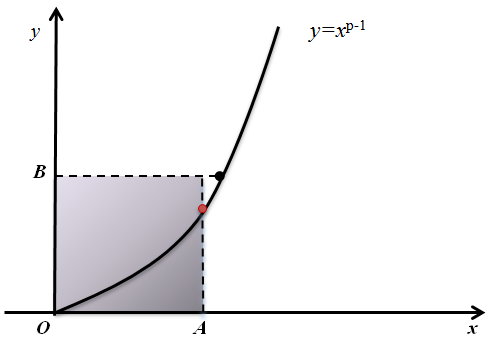
\includegraphics[width=0.65\textwidth]{image/holder.png}
\caption{~利用面积求不等式} \label{fig20}
\end{figure}

可知图~\ref{fig20}~中阴影区域面积恰为~$AB$, 且
\[
AB\leqslant \int_{0}^{A}x^{p-1}\mathrm{d} x+\int_{0}^{B}x^{q-1}\mathrm{d} x
\]
经计算得
\[
AB\leqslant \frac{A^{p}}{p}+\frac{B^{q}}{q}
\]

若~$f$~或~$g$~有一个为零函数, 则不等式~\eqref{equa2}~显然成立. 不妨设~$f$~和~$g$~都不是零函数, 从而
\[
\int_{a}^{b}|f(x)|^{p}\mathrm{d}\mu>0,\quad \int_{a}^{b}|g(x)|^{q}\mathrm{d}\mu>0
\]
由不等式~\eqref{equa3}, 可知
\[ \frac{|f(x)g(x)|}{\Big(\int_{a}^{b}|f(x)|^{p}\mathrm{d}\mu\Big)^{1/p}
\Big(\int_{a}^{b}|g(x)|^{q}\mathrm{d}\mu\Big)^{1/q}}
\leqslant \frac{1}{p}\frac{|f(x)|^{p}}{\int_{a}^{b}|f(x)|^{p}\mathrm{d}\mu}+\frac{1}{q}
\frac{|g(x)|^{q}}{\int_{a}^{b}|g(x)|^{q}\mathrm{d}\mu}
\]
将上式两端取积分后便可得所求不等式~\eqref{equa2}.
\end{proof}

\begin{Theorem}(\textbf{闵可夫斯基不等式}\index{闵可夫斯基不等式})
设~$p\geqslant 1$, $f,\, g\in L^p[a,\,b]$, 则
\begin{equation}\label{equa4}
\Big(\int_{a}^{b}|f(x)+g(x)|^{p}\mathrm{d}\mu\Big)^{\frac{1}{p}}\leqslant \Big(\int_{a}^{b}|f(x)|^{p}\mathrm{d}\mu\Big)^{\frac{1}{p}}+\Big(\int_{a}^{b}|g(x)|^{p}\mathrm{d}\mu\Big)^{\frac{1}{p}}
\end{equation}
\end{Theorem}

\begin{proof}
当~$p=1$~时, 定理显然成立. 设~$p>1$, $q$~为~$p$~的共轭数.

由定理~\ref{thm-2}, $(f(x)+g(x))\in L^p[a,\,b]$, 故~$|f(x)+g(x)|^{\frac{p}{q}}\in L_{q}[a,\,b]$.
将赫德尔不等式中~$g(x)$~换成~$|f(x)+g(x)|^{\frac{p}{q}}$, 可得
\[ \int_{a}^{b}|f(x)|\cdot|f(x)+g(x)|^{\frac{p}{q}}\mathrm{d}\mu
\leqslant \Big(\int_{a}^{b}|f(x)|^{p}\mathrm{d}\mu\Big)^{\frac{1}{p}}\Big(\int_{a}^{b}|f(x)+g(x)|^{p}\mathrm{d}\mu\Big)^{\frac{1}{q}}
\]
同理可知
\[
\int_{a}^{b}|g(x)|\cdot|f(x)+g(x)|^{\frac{p}{q}}\mathrm{d}\mu
\leqslant \Big(\int_{a}^{b}|g(x)|^{p}\mathrm{d}\mu\Big)^{\frac{1}{p}}\Big(\int_{a}^{b}|f(x)+g(x)|^{p}\mathrm{d}\mu\Big)^{\frac{1}{q}}
\]
又
\begin{eqnarray*}
|f(x)+g(x)|^{p}&=&|f(x)+g(x)||f(x)+g(x)|^{\frac{p}{q}}\\
&\leqslant& |f(x)|\cdot|f(x)+g(x)|^{\frac{p}{q}}+|g(x)|\cdot|f(x)+g(x)|^{\frac{p}{q}}
\end{eqnarray*}
因此
\begin{eqnarray*}\label{equa5}
\int_{a}^{b}|f(x)+g(x)|^{p}\mathrm{d}\mu &\leqslant& \Big(\int_{a}^{b}|f(x)|^{p}\mathrm{d}\mu\Big)^{\frac{1}{p}}\Big(\int_{a}^{b}|f(x)+g(x)|^{p}\mathrm{d}\mu\Big)^{\frac{1}{q}}\\
&& + \Big(\int_{a}^{b}|g(x)|^{p}\mathrm{d}\mu\Big)^{\frac{1}{p}}\Big(\int_{a}^{b}|f(x)+g(x)|^{p}\mathrm{d}\mu\Big)^{\frac{1}{q}}
\end{eqnarray*}

当~$\int_{a}^{b}|f(x)+g(x)|^{p}\mathrm{d}\mu\neq 0$~时, 在上述不等式两端都除以
~$\left(\int_{a}^{b}|g(x)|^{p}\mathrm{d}\mu\right)^{\frac{1}{p}}$, 即可得所求不等式~\eqref{equa4}; 当~$\int_{a}^{b}|f(x)+g(x)|^{p}\mathrm{d}\mu=0$~时, 不等式~\eqref{equa4}~自然成立. 定理证毕.
\end{proof}


\subsection*{二、$L^p$~空间的完备性与可分性}

\medskip

\qquad 设~$f(x)\in L^p[a,\,b]$, 定义
\[
\|f\|=\Big(\int_{a}^{b}f^{p}(x)\mathrm{d}\mu \Big)^{\frac{1}{p}}
\]
易知~$\|f\|$~满足范数定义中的性质~(i), (ii), 由闵可夫斯基不等式可知: $\|f\|$~亦满足范数定义中的性质~(iii). 因此, $\|f\|$~确为一范数.

\begin{Remark}
设~$f(x)$~为~$[a,\,b]$~上的可测函数, 若存在零测集~$E_0 \subset [a,\,b]$, 使得~$f(x)$~在~$[a,\,b]-E_0$~上有界．则称~$f(x)$~在~$[a,\,b]$~上本性有界\index{本性有界}. 记
\[
\mathop{\mathrm{ess}\sup}_{x \in [a,b]} f(x) =\inf_{E \subset [a,b] \atop m(E)=0} \Big\{ \sup_{t \in [a,b]-E} | f(x)| \Big\}
\]
称为~$f(x)$~在~$[a,\,b]$~上的本性上确界\index{本性上确界}.

$[a,\,b]$~上本性有界可测函数的全体, 记为~$L^\infty[a,\,b]$\index{$L^\infty$~空间}. 可以证明
\[
\lim_{p \to \infty} \|f\|_p = \|f\|_\infty
\]
事实上, 记~$M = \|f\|_\infty$, 则对任一满足~$M' < M$~的~$M'$, 点集
\[
A = \big\{ x \in [a,\,b]:\: |f(x)| > M'\big\}
\]
有正测度. 由不等式
\[
\|f\|_p = \Big( \int_a^b \big| f(x)\big|^p \mathrm{d} \mu \Big)^\frac{1}{p} \geqslant M' \big( m(A) \big)^\frac{1}{p}
\]
可知
\[
\liminf_{p \to \infty} \|f\|_p \geqslant M'
\]
令~$M' \to M$, 得
\[
\liminf_{p \to \infty} \|f\|_p \geqslant M
\]
另一方面, 我们总有
\[
\|f\|_p \leqslant \Big( \int_a^b M^p \mathrm{d} \mu \Big)^\frac{1}{p} = M \cdot (b-a)^\frac{1}{p}
\]
从而又得
\[
\liminf_{p \to \infty} \|f\|_p \geqslant M
\]
\end{Remark}

下面来看~$L^p[a,\,b]$~的完备性.

\begin{Definition}
设~$(X,\,\|\cdot\|)$~为赋范线性空间, 若对~$X$~中的任意柯西列~$\{x_n\}$, 都存在~$x \in X$, 使得~$x_n \xrightarrow {\|\cdot\|} x$. 则称~$X$~是完备\index{完备}的. 完备的赋范线性空间称为巴拿赫空间\index{巴拿赫空间}.
\end{Definition}

\begin{Theorem}
$L^p[a,\,b]$~空间是完备的, 即对任意柯西列~$\{f_n\} \subset L^p[a,\,b]$, 都存在~$f \in L^p[a,\,b]$~使得~$f_n \xrightarrow {\|\cdot\|} f$.
\end{Theorem}

\begin{proof}
设~$\{f_n\}\subset L^p[a,\,b]$~为柯西列, 则有
\[
\|f_{n}-f_{m}\|\rightarrow 0,\quad n,\,m\rightarrow \infty
\]
即对任意的~$k \in \N$, 存在正整数~$n_{k}$, 当~$n,\,m \geqslant n_{k}$~时, 有
\[
\|f_{n}-f_{m}\|\leqslant \frac{1}{2^{k}}
\]
不妨取~$n_{1}<n_{2}<\cdots$, 从而可得
\[
\sum_{k=1}^{\infty}\|f_{n_{k+1}}-f_{n_{k}}\|\leqslant \sum_{k=1}^{\infty}\frac{1}{2^{k}}=1
\]
令
\[
g_{m}(x)=|f_{n_{1}}(x)|+\sum_{k=1}^{m}|f_{n_{k+1}}(x)-f_{n_{k}}(x)|,\quad m=1,\,2,\,\cdots
\]
则~$g_{m}(x)\in L^p[a,\,b]$. 由范数的性质~(iii)~可知
\[
\|g_{m}\|\leqslant \|f_{n_{1}}\|+\sum_{k=1}^{m}\|f_{n_{k+1}}-f_{n_{k}}\|\leqslant \|f_{n_{1}}\|+1,\quad m=1,\,2,\,\cdots
\]

又~$g_{m}(x)\geqslant 0$~均是可测的, 由法都引理知
\begin{eqnarray*}
\int_{a}^{b}\liminf_{m \to \infty}g_{m}^{p}(x)\mathrm{d}\mu &\leqslant& \liminf_{m \to \infty}\int_{a}^{b}g_{m}^{p}(x)\mathrm{d}\mu \\
&=&\liminf_{m \to \infty}\|g_{m}\|^{p}\leqslant \big(\|f_{n_{1}}\|+1\big)^{p}
\end{eqnarray*}

由于~$\{g_{m}(x)\}$~是单调递增的函数列, 故~$\lim\limits_{m \to \infty}g_{m}(x)$~总存在(有限或者~$+\infty$). 从而
\[
\int_{a}^{b}\lim\limits_{m \to \infty}g_{m}^{p}(x)\mathrm{d}\mu\leqslant \big(\|f_{n_{1}}\|+1 \big)^{p}
\]
由此可知~$\lim\limits_{m \to \infty}g_{m}(x)$~是几乎处处有限的, 即
\[
|f_{n_{1}}(x)|+\sum_{k=1}^{\infty}|f_{n_{k+1}}(x)-f_{n_{k}}(x)|
\]
是几乎处处收敛的. 故函数列
\[
f_{n_{m+1}}(x)=f_{n_{1}}(x)+\sum_{k=1}^{m}(f_{n_{k+1}}(x)-f_{n_{k}}(x)),\quad m=1,\,2,\,\cdots
\]
也是几乎处处收敛的, 故存在几乎处处有限的可测函数~$f(x)$~使得
\[
\lim\limits_{m \to \infty}f_{n_{m}}(x)=f(x),\quad \mbox{~a.e.~} x\in \left[a,\,b\right]
\]
又
\begin{eqnarray*}
|f(x)|&\leqslant & |f_{n_{1}}(x)|+\sum_{k=1}^{\infty}|f_{n_{k+1}}(x)-f_{n_{k}}(x)|\\
&=& \lim\limits_{m \to \infty}g_{m}(x)
\end{eqnarray*}
可知~$f(x)\in L^p[a,\,b]$. 并且
\[
\|f-f_{n_{m}}\|\leqslant \sum_{k=m}^{\infty}\|f_{n_{k+1}}-f_{n_{k}}\| \longrightarrow 0,\quad m\rightarrow \infty
\]
由于
\[
\|f-f_{n}\|\leqslant \|f-f_{n_{m}}\|+\|f_{n}-f_{n_{m}}\|
\]
当~$n\rightarrow \infty$~时, 有
\[
\|f-f_{n}\|\rightarrow 0
\]
定理证毕.
\end{proof}
%%%%%%%%%%%%%%%%%%%%%%可分性%%%%%%%%%%%%%%%%%%%%%%%%%%%%%%%%%%%%%%%%%%%%%%%%%%%%%%%%%%%%%%%%%%%%%%%%

为得到空间~$L^p[a,\,b], p\geqslant 1$~的可分性, 先来介绍下面的一个著名定理:

\smallskip

定义在~$[a,\,b]$~上的所有连续函数的全体记为~$C[a,\,b]$, 设~$f(x)\in C[a,\,b]$, 定义
\[
\|f\|=\sup_{a\leqslant x\leqslant b}|f(x)|
\]
容易验证~$\|f\|$~满足范数定义的三条性质, 确为一范数.

\begin{Theorem}(\textbf{维尔斯特拉斯定理}\index{维尔斯特拉斯定理})
设~$f(x)$~为定义在~$[0,\,1]$~上的连续函数, 并有多项式
\[
B_{n}(x)=\sum_{k=0}^{n}\mathrm{C}_{n}^{k}f(\frac{k}{n})x^{k}(1-x)^{n-k},\quad n=1,\,2,\,\cdots
\]
则
\[
\|B_{n}-f\|=\sup_{0\leqslant  x\leqslant 1}|B_{n}(x)-f(x)| \longrightarrow 0
\]
\end{Theorem}

\begin{proof}
设
\[
b_{n,k}(x)=\mathrm{C}_{n}^{k}x^{k}(1-x)^{n-k},\quad k=1,\,2,\,\cdots, \,n
\]
对~$\forall x\in (0,\,1)$, 有
\[
\sum_{k=0}^{n}b_{n,k}(x)=1
\]
\begin{eqnarray*}
\sum_{k=0}^{n}k b_{n,k}(x)&=& nx\sum_{k=0}^{n}\frac{k}{n}\mathrm{C}_{n}^{k}x^{k-1}(1-x)^{n-k}\\
&=& nx\sum_{k=0}^{n-1}b_{n-1,k}(x)\\
&=& n x
\end{eqnarray*}
\[
\sum_{k=0}^{n}k(k-1) b_{n,k}(x)=n(n-1)x^{2}\sum_{k=0}^{n-2}b_{n-2,k}(x)=n(n-1)x^{2}
\]
因此
\begin{eqnarray*}
\sum_{k=0}^{n}(k-n x)^{2} b_{n,k}(x)&=& n^{2}x^{2}-(2nx-1)nx+n(n-1)x^{2}\\
&=& n x(1-x)
\end{eqnarray*}

由闭区间上连续函数的有界性和一致连续性可知, 存在~$M>0$~使得~$|f(x)|\leqslant M$, 且对任意的~$\varepsilon>0$, 存在~$\delta>0$, 对任意的~$x_{1},\, x_{2}\in [0,\,1]$,
当~$|x_{1}-x_{2}|<\delta$~时, 有
\[
|f(x_{1})-f(x_{2})|<\frac{\varepsilon}{2}
\]
取~$N=\big[M/(\delta^2\varepsilon)+1\big]$, 则
\begin{eqnarray*}
&&\big|B_{n}(x)-f(x)\big|= \Big|\sum_{k=0}^{n}\Big(f(\frac{k}{n})-f(x)\Big) b_{n,k}(x)\Big| \\
&=& \bigg|\sum_{\{k: |\frac{k}{n}-x|\leqslant \delta\}}\Big(f(\frac{k}{n})-f(x)\Big) b_{n,k}(x)+\sum_{\{k: |\frac{k}{n}-x|> \delta\}}\Big(f(\frac{k}{n})-f(x)\Big) b_{n,k}(x)\bigg|\\
&\leqslant& \frac{\varepsilon}{2}\cdot\sum_{k=0}^{n} b_{n,k}(x)+2M\sum_{\{k: |\frac{k}{n}-x|> \delta\}} b_{n,k}(x)\\
&\leqslant& \frac{\varepsilon}{2}+2M\sum_{k=0}^{n}\Big(\frac{k-n x}{n\delta}\Big)^{2}b_{n,k}(x)\\
&=& \frac{\varepsilon}{2}+\frac{2M}{n^{2}\delta^{2}}n x(1-x)\\
&\leqslant& \frac{\varepsilon}{2}+\frac{2M}{n\delta^{2}}\cdot\frac{1}{4} \\
&<&\varepsilon
\end{eqnarray*}
定理证毕.
\end{proof}

\begin{Definition}
设~$(X,\,\|\cdot\|)$~为赋范线性空间, 若~$X$~存在可数的稠密子集, 则称~$X$~是可分\index{可分}的.
\end{Definition}

若~$X$~可分, 则存在一列~$\{x_n\} \subset X$, 使得~$X$~中的每个元~$x$~可以用~$\{x_n\}$~中的元任意逼近, 即存在~$\{x_{n_k}\} \subset \{x_n\}$, 使得~$x_{n_k} \xrightarrow {\|\cdot\|} x$.

\begin{Theorem}
空间~$L^p[a,\,b], p\geqslant 1$~是可分的.
\end{Theorem}

\begin{proof}
对任意的~$f(x)\in L^p[a,\,b]$~及~$\varepsilon>0$, 可知存在有界可测函数列
~$\{f_{N}(x)\}\subset L^p[a,\,b]$~依范数收敛于~$f(x)$. 事实上, 由积分的绝对连续性, 对上述的~$\varepsilon>0$,
存在~$\delta>0$, 当~$m(E)<\delta$~时, 有
\[
\int_{a}^{b}|f(x)|^{p}\mathrm{d}\mu<(\frac{\varepsilon}{3})^{p}
\]
又因~$f(x)$~是几乎处处有限的可测函数, 故对上述的~$\delta>0$, 存在自然数~$N$, 使得
\[
m\big(\{x\in [a,\,b]:\: |f(x)|>N \}\big)<\delta
\]
令
\[
f_{N}(x)= \left\{\!\!
\begin{array}{cl}
f(x), & \quad |f(x)|<N \\[0.2cm]
0, & \quad |f(x)|\geqslant N
\end{array}
\right.
\]
显然, $f_{N}(x)\in L^p[a,\,b]$~是有界的, 且
\begin{eqnarray*}
\|f-f_{N}\|&=&\Big(\int_{a}^{b}|f(x)-f_{N}(x)|^{p}\mathrm{d}\mu\Big)^{\frac{1}{p}}\\
&=&\Big(\int_{\{x\in \left[a,\,b\right]:\: |f(x)|>N \}}|f(x)-f_{N}(x)|^{p}\mathrm{d}\mu\Big)^{\frac{1}{p}}<\frac{\varepsilon}{3}
\end{eqnarray*}
由卢津定理, 可知对每个有界可测函数~$f_{N}(x)$, 存在连续函数~$g_{N}(x)$~使得
\[
|g_{N}(x)|\leqslant N
\]
\[
m\big(\{x\in [a,\,b]:\: f_{N}(x)\neq g_{N}(x)\}\big)<\Big(\frac{\varepsilon}{6N}\Big)^{p}
\]
记~$E_0 = \{x\in [a,\,b]:\: f_{N}(x)\neq g_{N}(x)\}$, 从而
\begin{eqnarray*}
\|f_{N}-g_{N}\| &=& \Big(\int_{a}^{b}|f_{N}(x)-g_{N}(x)|^{p}\mathrm{d}\mu\Big)^{\frac{1}{p}}\\
&=&\left(\int_{E_0}|f_{N}(x)-g_{N}(x)|^{p}\mathrm{d}\mu\right)^{\frac{1}{p}}\\
&\leqslant& \Big(\int_{E_0}|f_{N}(x)|^{p}\mathrm{d}\mu\Big)^{\frac{1}{p}}
+ \Big(\int_{E_0}|g_{N}(x)|^{p}\mathrm{d}\mu\Big)^{\frac{1}{p}}\\
&\leqslant& \big[N^{p}\cdot m\big(E_0\big)\big]^{\frac{1}{p}}
+\big[N^{p}\cdot m\big(E_0\big)\big]^{\frac{1}{p}} \\
&<&\frac{\varepsilon}{3}
\end{eqnarray*}
再根据维尔斯特拉斯定理, 连续函数~$g_{N}(x)$~可由有理系数多项式一致逼近, 即存在有理系数多项式~$P_{N}(x)$~使得
\[
\max_{x\in [a,\,b]}|g_{N}(x)-P_{N}(x)|<\frac{\varepsilon}{3(b-a)^{1/p}}
\]
从而
\[
\|g_{N}-P_{N}\|=\Big(\int_{a}^{b}|g_{N}(x)-P_{N}(x)|^{p}\mathrm{d}\mu\Big)^{\frac{1}{p}}\leqslant \frac{\varepsilon}{3}
\]
则
\begin{eqnarray*}
\|f-P_{n}\|&\leqslant& \|f-f_{N}\|+\|f_{N}-g_{N}\|+\|g_{N}-P_{N}\|\\
&<&\frac{\varepsilon}{3}+\frac{\varepsilon}{3}+\frac{\varepsilon}{3}=\varepsilon
\end{eqnarray*}
因此, $[a,\,b]$~上的有理系数多项式在~$L^p[a,\,b]$~上是稠密的, 而所有有理系数多项式构成的集合是可数的, 故定理成立.
\end{proof}

\newpage

\vspace*{-0.6cm}

\section*{第六章习题}

%\addcontentsline{toc}{section}{~~~~~第六章习题}

\begin{enumerate}

\item 设~$f_{n}(x), f(x)\in L^2[a,\,b]$, $f_{n}$~依测度收敛于~$f$, 若存在~$M>0$~使得~$\|f_{n}\|\leqslant M$, 试证明~$f_{n}$~弱收敛于~$f$.

\item 设~$f_{n}(x), f(x)\in L^2[a,\,b]$, $f_{n}$~弱收敛于~$f$, 则存在~$M>0$~使得~$\|f_{n}\|\leqslant M$.

\item 举例说明~$L^2[a,\,b]$~中的弱收敛函数列未必是依测度收敛的.

\item 若对任意的~$f(x)\in L^2[a,\,b]$, 都有
\[
\int_{a}^{b}f(x)g(x)\mathrm{d}\mu<\infty
\]
则~$g(x) \in L^2[a,\,b]$.

\item 设~$f_{n}(x), f(x)\in L^2[a,\,b]$, $f_{n}$~弱收敛于~$f$, 且~$\|f_{n}\|\rightarrow \|f\|$, 则~$f_{n}$~依范数收敛于~$f$.

\item 试证明~$L^2[a,\,b]$~中的规范正交系至多是可数的.

\item 设~$\{g_{n}(x)\}$~是定义在~$\left[a,\,b\right]$~上封闭的规范正交系, 则~$\sum\limits_{n=1}^{\infty}g_{n}^{2}(x)=+\infty$~在~$\left[a,\,b\right]$~上几乎处处成立.


\item 设~$\{g_{n}(x)\}\subset L^2[a,\,b]$~是完全的规范正交系, 若~$\{\varphi_{n}(x)\}\subset L^2[a,\,b]$~满足
\[
\sum_{n=1}^{\infty}\int_{a}^{b}[g_{n}(x)-\varphi_{n}(x)]^{2}\mathrm{d}\mu<1
\]
则~$\{\varphi_{n}(x)\}$~也是完全的.

\item 试证明~$L^2[a,\,b]$~中有限的函数系不是完全的.

\item 设~$\{g_{n}(x)\}\subset L^2[a,\,b]$~是一规范正交系, $f(x)\in L^2[a,\,b]$. 对线性组合~$\sum\limits_{k=1}^{n}a_{k}g_{k}(x)$~作范数
\[
\Big\|f-\sum_{k=1}^{n}a_{k}g_{k}\Big\|
\]
则当~$a_{k}=(f,g_{k})$~时, 上述范数取最小值.

\item 试证明~$L^p[a,\,b], p\geqslant 1$~是完全的.

\item 设~$f\in L^p[a,\,b]\cap L^{p'}\left[a,\,b\right]$, $1\leqslant p<r<p'$, 试证明~$f\in L^{r}\left[a,\,b\right]$.

\item 设~$f \in L^p(E)$, $e \subset E$~可测, 证明
\[
\Big( \int_E |f(x)|^p \mathrm{d} \mu \Big)^\frac{1}{p} \leqslant \Big( \int_e |f(x)|^p \mathrm{d} \mu \Big)^\frac{1}{p} + \Big( \int_{E-e} |f(x)|^p \mathrm{d} \mu \Big)^\frac{1}{p}
\]

\item 设~$f \in L^p(-\infty,\,+\infty),\,g\in L^q(-\infty,\,+\infty)$, 其中~$\frac{1}{p}+\frac{1}{q} =1,\,p\geqslant 1$, 试证
    \[
    F(t)=\int_{-\infty}^{+\infty} f(x+t)g(x) \mathrm{d} \mu
    \]
    为~$t$~的连续函数.

\item 设~$f_{n}(x),\, f(x)\in L^p[a,\,b], p\geqslant 1$, 若~$f_{n}\xrightarrow{\mathrm{\|\cdot\|}} f$, 则~$\{f_n\}$~是柯西列.

\item 设~$f_{n}(x),\, f(x)\in L^p[a,\,b], p\geqslant 1$, 若~$f_{n}\xrightarrow{\mathrm{\|\cdot\|}} f$, 则~$\|f_n\|\rightarrow \|f\|$.

\item $L^p[a,\,b], p\geqslant 1$~中的函数列在依范数收敛的意义下, 极限函数是唯一的.

\item 设~$f\in L^p[a,\,b], p\geqslant 1$, 则对任意~$\varepsilon>0$, 存在有界可测函数~$g$~使得
\[
\|f-g\|<\varepsilon
\]

\item 设~$f\in L^p[a,\,b], p\geqslant 1$, 则对任意~$\varepsilon>0$, 存在连续函数~$F$~使得
\[
\|f-F\|<\varepsilon
\]

\end{enumerate}
% \chapter*{附 \ \ 录}
\addcontentsline{toc}{chapter}{\protect\numberline{附 \ \ 录}{}}
\markboth{附 \ \ 录}{附 \ \ 录}

\setcounter{chapter}{7}
\setcounter{Theorem}{0}
\setcounter{Definition}{0}
\setcounter{Proposition}{0}
\setcounter{Corollary}{0}
\setcounter{Remark}{0}
\setcounter{Lemma}{0}

\bigskip

\bigskip


\section*{斯蒂尔杰斯积分简介}

\setcounter{section}{1}

\bigskip

\subsection*{一、引言}

\qquad 对于连续函数~$g(x)$~的积分
\[
\int_0^1 g(x) \mathrm{d} x
\]
可以看作是~$g(x)$~在~$[0,\,1]$~上的平均值. 在某些情形下, 考虑~$g$~的不同的平均也是重要的, 它反映了~$g$~在~$[0,\,1]$~内各个地方的不同作用与影响. 例如考虑
\[
\int_0^1 g(x) x^2 \mathrm{d} x
\]
也是~$g$~的一种平均, 但此时在~$[0,\,1]$~中接近~$1$~的点与接近~$0$~的点上, 对~$g$~求平均的份量是不同的. 这种``偏重''的平均一般用一个``权''函数
\[
w:\:[0,\,1] \rightarrow [0,\,+\infty]
\]
来描述, 即~$g$~在~$[0,\,1]$~上的加权~$w$~平均为
\[
\int_0^1 g(x)w(x) \mathrm{d} x \Big/ \int_0^1 w(x) \mathrm{d} x
\]
有时我们还要考虑取平均时, 其权仅集中在某些点上, 如~$g(1/4)2 + g(3/4)2$.
这种情况相当于区间~$[0,\,1/4)$, $(1/4,\,3/4)$~以及~$(3/4,\,1]$~对积分没有贡献, 也可以说类似于某种零测集.
一般这一问题可描述为
\[
\sum_{n=1}^\infty p_n g(a_n), \quad a_n \in [0,\,1], \quad n=1,\,2,\,\cdots
\]
其中, $p_n \geqslant 0,\,\forall~n \in \N$~且~$\sum\limits_{n=1}^\infty p_n=1$.

下面我们来建立一种叫作斯蒂尔杰斯积分的理论, 在这一理论中, 上述种种情况将是
这一理论的特殊情形.

\medskip

\subsection*{二、黎曼\raisebox{0.5mm}{--}斯蒂尔杰斯积分}

\begin{Definition}
设~$g(x),\,f(x)$~为定义在~$[a,\,b]$~上的实值函数, 对于~$[a,\,b]$~的分割~$\mathrm{d}elta:\: a=x_0 < x_1 < \cdots < x_n =b$, 记
\[
\|\mathrm{d}elta\|=\max\{|x_i-x_{i-1}|: \: 1 \leqslant i \leqslant n\}
\]
任取~$\xi_i \in [x_{i-1},\,x_i], \, i=1,\,\cdots,\,n$, 若极限
\[
\lim_{\|\mathrm{d}elta\| \to 0} \sum_{i=1}^n g(\xi_i)[f(x_i)-f(x_{i-1})]
\]
存在, 记为~$I$, 则称该极限为~$g$~关于~$f$~在~$[a,\,b]$~上的黎曼\raisebox{0.5mm}{--}斯蒂尔杰斯积分\index{黎曼\raisebox{0.5mm}{--}斯蒂尔切斯积分}, 简称~R-S~积分, 记为
\[
I = \int_a^b g(x) \mathrm{d} f(x)
\]
\end{Definition}

注意, 要保证~$\int_a^b g(x) \mathrm{d} f(x)$~存在, 必须要求~$f$~与~$g$~在~$[a,\,b]$~上不能有公共不连续点(证明可参考文献~\cite{zhou}).

\begin{Remark}
(i) 若取~$f(x)=x$, 则~R-S~积分即为~R-积分;

(ii) 若~$f(x)$~是绝对连续的单调递增函数, 则~$\int_a^b \mathrm{d} f(x) = \int_a^b f'(x) \mathrm{d} \mu$, 故~R-S~积分变为~L-积分.
\end{Remark}

\begin{Proposition}
R-S~积分满足下列性质:

(i) 若~$\int_a^b g(x) \mathrm{d} f(x)$~存在, $c$~是常数, 则~$\int_a^b cg(x) \mathrm{d} f(x)$~与~$\int_a^b g(x) \mathrm{d} \big(cf(x)\big)$~存在, 且
\[
\int_a^b cg(x) \mathrm{d} f(x) = \int_a^b g(x) \mathrm{d} \big(cf(x)\big) = c\int_a^b g(x) \mathrm{d} f(x)
\]

(ii) 若~$\int_a^b g_1(x) \mathrm{d} f(x), \,\int_a^b g_2(x) \mathrm{d} f(x)$~存在, 则~$\int_a^b [g_1(x) + g_2(x)] \mathrm{d} f(x)$~存在, 且
\[
\int_a^b [g_1(x) + g_2(x)] \mathrm{d} f(x) = \int_a^b g_1(x) \mathrm{d} f(x) + \int_a^b g_2(x) \mathrm{d} f(x)
\]

(iii) 若~$\int_a^b g(x) \mathrm{d} f_1(x), \,\int_a^b g(x) \mathrm{d} f_2(x)$~存在, 则~$\int_a^b g(x) \mathrm{d} [f_1(x)+f_2(x)]$~存在, 且
\[
\int_a^b g(x) \mathrm{d} [f_1(x)+f_2(x)] = \int_a^b g(x) \mathrm{d} f_1(x) + \int_a^b g(x) \mathrm{d} f_2(x)
\]
\end{Proposition}

\begin{Proposition}
设~$\int_a^b g(x) \mathrm{d} f(x)$~存在, $c \in (a,\,b)$, 则~$\int_a^c g(x) \mathrm{d} f(x)$~与~$\int_c^b g(x) \mathrm{d} f(x)$~都存在, 且
\[
\int_a^b g(x) \mathrm{d} f(x) = \int_a^c g(x) \mathrm{d} f(x) + \int_c^b g(x) \mathrm{d} f(x)
\]
\end{Proposition}

\begin{Remark}
设~$f(x),\,g(x)$~为定义在~$[a,\,b]$~上的实值函数, 若对于~$c \in (a,\,b)$, 已知~$\int_a^c g(x) \mathrm{d} f(x), \, \int_c^b g(x) \mathrm{d} f(x)$~存在, 并不能推出~$\int_a^b g(x) \mathrm{d} f(x)$~存在.

例如, 令
\[
g(x)=\chi_{[0,1]}(x), \quad f(x)= \chi_{[0,1]}(x)
\]
易知
\[
\int_0^1 g(x) \mathrm{d} f(x) = 0, \quad \int_{-1}^0 g(x) \mathrm{d} f(x) = 0
\]
但积分~$\int_{-1}^1 g(x) \mathrm{d} f(x)$~并不存在. 不过下面结论成立:

\smallskip

若~$f(x)$~为~$[a,\,b]$~上的有界函数, 设~$c \in (a,\,b)$, $g(x)$~在~$x=c$~处连续, 则当~$\int_a^c g(x) \mathrm{d} f(x), \, \int_c^b g(x) \mathrm{d} f(x)$~存在时, 有积分~$\int_a^b g(x) \mathrm{d} f(x)$~存在.
\end{Remark}

在~R-S~积分定义中, 记
\[
S_\mathrm{d}elta = \sum_{i=1}^n g(\xi_i)[f(x_i)-f(x_{i-1})]
\]
称为关于分割~$\mathrm{d}elta$~的黎曼\raisebox{0.5mm}{--}斯蒂尔杰斯和式, 简称~R-S~和式.

\begin{Theorem} \label{thm711}
R-S~积分~$\int_a^b g(x) \mathrm{d} f(x)$~存在的充要条件是, 对~$\forall~\varepsilon > 0$, 存在~$\mathrm{d}elta > 0$, 使得当任意两个分割~$\mathrm{d}elta'$~与~$\mathrm{d}elta''$~满足~$\|\mathrm{d}elta'\|<\mathrm{d}elta,\,\|\mathrm{d}elta''\|<\mathrm{d}elta$~时, 都有
\[
|S_{\mathrm{d}elta'} - S_{\mathrm{d}elta''}| < \varepsilon
\]
\end{Theorem}

\begin{Theorem}
设~$\int_a^b g(x) \mathrm{d} f(x)$~存在, 则~$\int_a^b f(x) \mathrm{d} g(x)$~也存在, 且
\begin{equation} \label{eq711}
\int_a^b g(x) \mathrm{d} f(x) = [g(b)f(b)-g(a)f(a)]-\int_a^b f(x) \mathrm{d} g(x)
\end{equation}
\end{Theorem}

\begin{proof}
对于分割~$\mathrm{d}elta:\: a=x_0 < x_1 <\cdots < x_n =b$, 以及任意的~$\xi_i \in [x_{i-1},\,x_i], \, i=1,\,\cdots,\,n$, 有
\begin{eqnarray*}
S_\mathrm{d}elta &=& \sum_{i=1}^n g(\xi_i)[f(x_i)-f(x_{i-1})] \\
&=& \sum_{i=1}^n g(\xi_i)f(x_i) - \sum_{i=1}^n g(\xi_i)f(x_{i-1}) \\
&=& - \sum_{i=1}^n f(x_i) [g(\xi_{i+1})-g(\xi_i)] + g(\xi_n)f(b)-g(\xi_1)f(a) \\
&=& -T_{\mathrm{d}elta} + [g(b)f(b)-g(a)f(a)]
\end{eqnarray*}
其中
\[
T_\mathrm{d}elta=\sum_{i=1}^n f(x_i) [g(\xi_{i+1})-g(\xi_i)]+f(a)[g(\xi_1)-g(a)]+f(b)[g(b)-g(\xi_n)]
\]
是~$f(x)$~关于~$g(x)$~在~$[a,\,b]$~上的~R-S~和式. 由于分割~$\mathrm{d}elta$~是任意的, 令~$\|\mathrm{d}elta\| \to 0$~可得, $\int_a^b f(x) \mathrm{d} g(x)$~存在, 且式~\eqref{eq711}~成立.
\end{proof}

R-S~积分~$\int_a^b g(x) \mathrm{d} f(x)$~的一个最重要的特例是~$f(x)$~为单调函数或有界变差函数的情形.

设~$g(x)$~为~$[a,\,b]$~上的有界实值函数, $f(x)$~为~$[a,\,b]$~上的单调递增函数, 对于分割~$\mathrm{d}elta: \:  a=x_0 < x_1 <\cdots < x_n =b$, 记
\[
m_i=\inf\{g(x):\: x_{i-1} \leqslant x \leqslant x_i\}, \, \quad M_i = \sup\{g(x): \: x_{i-1} \leqslant x \leqslant x_i\}
\]
\[
L_\mathrm{d}elta = \sum_{i=1}^n m_i [f(x_i)-f(x_{i-1})], \quad U_\mathrm{d}elta = \sum_{i=1}^n M_i [f(x_i)-f(x_{i-1})]
\]
则显然有~$L_\mathrm{d}elta \leqslant S_\mathrm{d}elta \leqslant U_\mathrm{d}elta$, 且易证:

(i) 若~$\mathrm{d}elta'$~是~$\mathrm{d}elta$~的加细, 则~$L_{\mathrm{d}elta'} \geqslant L_\mathrm{d}elta,\, U_{\mathrm{d}elta'} \leqslant U_\mathrm{d}elta$;

(ii) 若~$\mathrm{d}elta',\,\mathrm{d}elta''$~是任意两个分割, 则~$L_{\mathrm{d}elta'} \leqslant U_{\mathrm{d}elta''}$, 且~R-S~积分存在当且仅当
\[
\lim_{\|\mathrm{d}elta\| \to 0} L_\mathrm{d}elta = \lim_{\|\mathrm{d}elta\| \to 0} S_\mathrm{d}elta = \lim_{\|\mathrm{d}elta\| \to 0} U_\mathrm{d}elta ~(~= I~)
\]

\begin{Theorem}
设~$g(x)$~为~$[a,\,b]$~上的连续函数, $f(x)$~是~$[a,\,b]$~上的有界变差函数, 则~$\int_a^b g(x) \mathrm{d} f(x)$~存在, 且
\begin{equation} \label{eq712}
\Big| \int_a^b g(x) \mathrm{d} f(x) \Big| \leqslant \sup_{x \in [a,b]} \big| g(x) \big| \cdot \biancha\limits_a^b(f)
\end{equation}
\end{Theorem}

\begin{proof}
先证明积分~$\int_a^b g(x) \mathrm{d} f(x)$~的存在性, 不妨假设~$f(x)$~是单调递增函数, 由定理~\ref{thm711}~只需证明极限~
$\lim\limits_{\|\mathrm{d}elta\| \to 0} L_\mathrm{d}elta$~和~$\lim\limits_{\|\mathrm{d}elta\| \to 0} U_\mathrm{d}elta$~存在且相等.

若~$f(x)$~是常数函数, 则结论显然成立. 否则, 由~$g(x)$~的连续性知, 对任给的~$\varepsilon > 0$, 存在~$\mathrm{d}elta > 0$, 只要分割~$\mathrm{d}elta$~满足~$\|\mathrm{d}elta\| < \mathrm{d}elta$, 就有
\[
M_i-m_i < \frac{\varepsilon}{f(b)-f(a)}
\]
于是, 当~$\|\mathrm{d}elta\| < \mathrm{d}elta$~时, 有
\[
U_\mathrm{d}elta - L_\mathrm{d}elta = \sum_{i=1}^n (M_i-m_i) [f(x_i)-f(x_{i-1})] < \varepsilon
\]
这说明
\begin{equation} \label{eq713}
\lim_{\|\mathrm{d}elta\| \to 0} (U_\mathrm{d}elta-L_\mathrm{d}elta) = 0
\end{equation}
下面证明~$\lim\limits_{\|\mathrm{d}elta\| \to 0} U_\mathrm{d}elta$~存在. 若不然, 则存在~$\varepsilon_0 > 0$~以及分割列~$\{\mathrm{d}elta_k'\}$~与~$\{\mathrm{d}elta_k''\}$, 满足~$\|\mathrm{d}elta_k'\|$~与~$\|\mathrm{d}elta_k''\| \to 0, \, k \to \infty$, 且
\[
U_{\mathrm{d}elta_k'} - U_{\mathrm{d}elta_k''} > \varepsilon_0
\]
从而由式~\eqref{eq713}~知, 当~$k$~足够大时有
\[
L_{\mathrm{d}elta_k'}-U_{\mathrm{d}elta_k''} > \frac{\varepsilon}{2} > 0
\]
这与分割的性质~$L_{\mathrm{d}elta'} \leqslant U_{\mathrm{d}elta''}$~矛盾.

最后, 由于对任意的分割~$\mathrm{d}elta$, 都有
\begin{eqnarray*}
S_\mathrm{d}elta \leqslant U_\mathrm{d}elta &=& \sum_{i=1}^n M_i [f(x_i)-f(x_{i-1})] \\
&\leqslant& \sup_{x \in [a,b]} \big| g(x) \big| \sum_{i=1}^n \big|f(x_i)-f(x_{i-1})\big|
\end{eqnarray*}
两边关于~$\mathrm{d}elta$~取极限可得不等式~\eqref{eq712}.
\end{proof}

\begin{Example}
设~$f(x)$~在~$\R^n$~的一个球层~$a \leqslant \|x\| \leqslant b$~上是可积的, $g\big(\|x\|\big)=g(r)$~是~$a \leqslant r \leqslant b$~上的连续函数, 其中~$0 \leqslant a < b < +\infty$. 若令
\[
F(r)=\int_{a\leqslant \|x\| \leqslant r} f(x) \mathrm{d} x, \quad a \leqslant r \leqslant b
\]
则有
\[
\int_{a \leqslant \|x\| \leqslant b} f(x) g\big(\|x\|\big) \mathrm{d} x = \int_a^b g(r) \mathrm{d} F(r)
\]
\end{Example}

\begin{proof}
先证上式右端的积分存在. 不妨设~$f(x) \geqslant 0$, 并记上式左端为~$I$. 作区间~$[a,\,b]$~的分割~$\mathrm{d}elta: \: a=r_0 < r_1 < \cdots < r_k = b$. 则有
\[
I = \sum_{i=1}^k \int_{r_{i-1} \leqslant \|x\| \leqslant r_i} f(x) g\big(\|x\|\big) \mathrm{d} x
\]
对每个~$i=1,\,\cdots,\,k$, 令
\[
m_i=\inf\{g(r):\: r_{i-1} \leqslant r \leqslant r_i\}, \quad M_i=\sup\{g(r):\: r_{i-1} \leqslant r \leqslant r_i\}
\]
则由~$f \geqslant 0$~可知
\[
\sum_{i=1}^k m_i \int_{r_{i-1} \leqslant \|x\| \leqslant r_i} f(x) \mathrm{d} x \leqslant I \leqslant \sum_{i=1}^k m_i \int_{r_{i-1} \leqslant \|x\| \leqslant r_i} f(x) \mathrm{d} x
\]
从而
\[
\sum_{i=1}^k m_i \big[ F(r_i)-F(r_{i-1}) \big] \leqslant I \leqslant \sum_{i=1}^k M_i \big[ F(r_i)-F(r_{i-1}) \big]
\]
由~R-S~积分的定义, 当~$\|\mathrm{d}elta\| \to 0$~时, 上式两端都趋于~$\int_a^b g(x) \mathrm{d} F(r)$. 因此, $I = \int_a^b g(r) \mathrm{d} F(r)$.
\end{proof}

\subsection*{三、勒贝格\raisebox{0.5mm}{--}斯蒂尔杰斯测度与积分}

\qquad 下面在~$\R$~上建立一种新的测度、积分理论\raisebox{0.5mm}{-----}勒贝格\raisebox{0.5mm}{--}斯蒂尔杰斯测度、积分理论, 它在概率论中有着非常重要的应用, 本书正文中所讲的勒贝格测度、积分是它的一种特殊情形.

我们还将讨论这种勒贝格\raisebox{0.5mm}{--}斯蒂尔杰斯积分与黎曼\raisebox{0.5mm}{--}斯蒂尔杰斯积分的关系, 并从
勒贝格\raisebox{0.5mm}{--}斯蒂尔杰斯测度的角度给出一个函数是黎曼\raisebox{0.5mm}{--}斯蒂尔杰斯可积的充要条件.

\begin{Definition}
设~$f(x)$~为~$\R$~上单调递增的实值函数, 对~$\R$~中非空子集~$E$, 令
\[
\mu_f^*(E)=\inf\Big\{ \sum_k [f(b_k)-f(a_k)]: \: E \subset \medcup_k(a_k,\,b_k] \Big\}
\]
并规定~$\mu_f^*(\emptyset)=0$. 下列事实成立:

(i)(\textbf{非负性}) $\mu_f^*(E) \geqslant 0$;

(ii)(\textbf{单调性}) 若~$E_1 \subset E_2$, 则~$\mu_f^*(E_1) \leqslant \mu_f^*(E_2)$;

(iii)(\textbf{次可加性}) $\mu_f^*\big(\smallcup\limits_{n=1}^\infty E_n \big) \leqslant \sum\limits_{n=1}^\infty \mu_f^*(E_n)$.

\smallskip

这说明~$\mu_f^*(\cdot)$~是定义在~$\R$~上的外测度, 称为相应于~$f$~的
勒贝格--斯蒂尔杰斯外测度\index{勒贝格--斯蒂尔杰斯外测度}, 简称~L-S~外测度.
\end{Definition}

若取~$f(x)=x$, L-S~外测度就是勒贝格外测度.

\begin{Theorem} \label{thm714}
设~$E_1,\,E_2$~为~$\R$~中的点集, 若~$d(E_1,\,E_2) > 0$, 则
\[
\mu_f^*(E_1) + \mu_f^*(E_2) = \mu_f^*\big(E_1 \medcup E_2\big)
\]
\end{Theorem}

\begin{proof}
注意到, 若~$a = a_0 < a_1 < \cdots < a_n =b$, 则有
\[
f(b)-f(a) = \sum_{i=1}^n [f(a_i)-f(a_{i-1})]
\]
故在~$\mu_f^*$~的定义中, 可以使每个覆盖子区间~$(a_k,\,b_k]$~取的充分小, 从而对任意的~$\varepsilon > 0$, 我们选取~$\big\{(a_k,\,b_k]\big\}$, 其中每个~$(a_k,\,b_k]$~的长度小于~$d(E_1,\,E_2)$, 使得~$E_1 \smallcup E_2 \subset \mathop{\textstyle{\smallcup}}\limits_k(a_k,\,b_k]$, 且
\[
\sum_k [f(b_k)-f(a_k)] \leqslant \mu_f^*\big( E_1 \medcup E_2 \big) + \varepsilon
\]
于是再把~$\big\{(a_k,\,b_k]\big\}$~分为两个覆盖族, 其一覆盖~$E_1$, 其二覆盖~$E_2$, 就可以得到
\[
\mu_f^*(E_1)+\mu_f^*(E_2) \leqslant \sum_k [f(b_k)-f(a_k)] \leqslant \mu_f^* \big(E_1 \medcup E_2 \big) + \varepsilon
\]
由~$\varepsilon$~的任意性可知
\[
\mu_f^*(E_1)+\mu_f^*(E_2) \leqslant \mu_f^*\big(E_1 \medcup E_2 \big)
\]
而相反的不等式可由~L-S~外测度的次可加性得到.
\end{proof}

有了~L-S~外测度, 再借助卡拉西尔德瑞条件就可以定义~L-S~可测集.

\begin{Definition}
若对任意的点集~$T \subset \R$, 都有
\[
\mu_f^*(T)=\mu_f^*\big(T \medcap E\big) + \mu_f^*\big(T \medcap E^c\big)
\]
则称~$E$~为~$\R$~中的~$\mu_f$~可测集\index{勒贝格\raisebox{0.5mm}{--}斯蒂尔切斯可测集}, 此时其测度称为勒贝格--斯蒂尔杰斯测度\index{勒贝格\raisebox{0.5mm}{--}斯蒂尔切斯测度}, 简称~L-S~测度, 记为~$\mu_f(E)$.
\end{Definition}

$\R$~中的可测集也构成一个~$\sigma$-代数. 由此可知, 为了证明~$\R$~中的波雷尔集都是~L-S~可测集, 只需证明~$\R$~中的区间是~L-S~可测集即可, 而~$\mu_f$~继承自~$\mu_f^*$~的距离外测度性质
(定理~\ref{thm714})可以保证这点.

\begin{Theorem}
设~$E \subset \R$, 则存在波雷尔集~$B: \: B \supset E$, 使得~$\mu_f^*(E)=\mu_f(B)$.
\end{Theorem}

\begin{proof}
对每个~$n \in \N$, 选取~$\big\{ (a_k^{(n)},\,b_k^{(n)}] \big\}$~满足
\[
E \subset \mathop{\textstyle{\medcup}}_k (a_k^{(n)},\,b_k^{(n)}], \quad
\sum_k \big[ f(b_k^{(n)})-f(a_k^{(n)}) \big] \leqslant \mu_f^*(E) + \frac{1}{n}
\]
令
\[
B_n = \mathop{\textstyle{\medcup}}_k (a_k^{(n)},\,b_k^{(n)}], \quad B =  \mathop{\textstyle{\medcap}}_n B_n
\]
则~$E \subset B$, 且~$B$~是波雷尔集. 从而
\[
\mu_f(B) \leqslant \mu_f(B_n) \leqslant \sum_k \big[ f(b_k^{(n)})-f(a_k^{(n)}) \big] \leqslant \mu_f^*(E) + \frac{1}{n}
\]
令~$n \to \infty$~得~$\mu_f(B) \leqslant \mu_f^*(E)$. 而相反的不等式是显然的.
\end{proof}

\begin{Proposition}
若~$f(x)$~为~$\R$~上单调递增的右连续函数, 则
\[
\mu_f\big( (a,\,b] \big) = f(b)-f(a)
\]
特别地, $\mu_f\big( \{a\} \big) = f(a) - f(a-0)$.
\end{Proposition}

\begin{proof}
由于~$(a,\,b]$~是其自身的一个覆盖, 故总有
\[
\mu_f\big( (a,\,b] \big) \leqslant f(b)-f(a)
\]
另一方面, 设~$(a,\,b] \subset \smallcup\limits_k (a_k,\,b_k]$, 对任意的~$\varepsilon > 0$, 由于~$f$~的右连续性, 故可选取~$\{b_k'\}$~使得
\[
b_k < b_k', \quad f(b_k) > f(b_k') - \frac{\varepsilon}{2^k}
\]
若~$a'$~满足~$a < a' < b$, 则~$\big\{(a_k,\,b_k')\big\}$~覆盖~$[a',\,b]$, 从而存在有限子覆盖, 不妨设
\[
[a',\,b] \subset \medcup_{k=1}^m (a_k,\,b_k')
\]
可以假定~$a_{k+1} < b_k', \, k=1,\,\cdots,\,m-1$ (必要时剔除一部分区间), 且~$a_1 < a',\, b < b_m'$. 从而
\[
f(a_1) \leqslant f(a'), \quad f(b) \leqslant f(b_m')
\]
\begin{eqnarray*}
\sum_k \big[ f(b_k)-f(a_k)\big] &\geqslant& \sum_{k=1}^m \big[ f(b_k)-f(a_k)\big] \\
&=& f(b_m)-f(a_1) + \sum_{k=1}^{m-1} \big[ f(b_k)-f(a_{k+1})\big]
\end{eqnarray*}
注意到
\begin{eqnarray*}
f(b_m)-f(a_1) &=& \big[f(b_m)-f(b_m')\big] + \big[f(b_m')-f(a_1)\big] \\
&\geqslant& -\varepsilon + \big[f(b)-f(a')\big]
\end{eqnarray*}
\[
f(b_k')-f(a_{k+1}) \geqslant 0, \quad k=1,\,\cdots,\,m-1
\]
于是
\begin{eqnarray*}
\sum_{k=1}^{m-1} \big[ f(b_k)-f(a_{k+1})\big] &=& \sum_{k=1}^{m-1} \big[ f(b_k)-f(b_k')\big] + \sum_{k=1}^{m-1} \big[ f(b_k')-f(a_{k+1})\big] \\
&\geqslant& \sum_{k=1}^{m-1} \frac{-\varepsilon}{2^k} \geqslant -\varepsilon
\end{eqnarray*}
因此
\[
\sum_k \big[ f(b_k)-f(a_k)\big] \geqslant -2 \varepsilon + \big[ f(b)-f(a') \big]
\]
令~$\varepsilon \to 0, \, a' \to a$~可得
\[
\sum_k \big[ f(b_k)-f(a_k)\big] \geqslant f(b)-f(a)
\]
即~$\mu_f\big( (a,\,b] \big) = f(b)-f(a)$.

\smallskip

第二部分的结论, 只要应用上述过程于~$(a-1/k,\,a],\ k=1,\,2,\,\cdots$~即可.
\end{proof}

\begin{Remark}
在~L-S~外测度的定义中, 若采用开区间代替半开半闭区间, 即令
\[
\mu_f^*(E)=\inf\Big\{ \sum_k [f(b_k)-f(a_k)]: \: E \subset \medcup_k(a_k,\,b_k) \Big\}
\]
则不难证明~$\mu_f^*$~是~$\R$~上的距离外测度, 且有

\noindent(i) $\mu_f^*(E) = \inf\big\{ \mu_f^*(G): \: G \supset E,\, G \mbox{~开} \big\}$;

\noindent(ii) 下列关系成立
 \[
 \mu_f^*\big( \{a\} \big) = f(a+0)-f(a-0)
 \]
 \[
 \mu_f^*\big( [a,\,b] \big) = f(b+0)-f(a-0)
 \]
 \[
 \mu_f^*\big( (a,\,b] \big) = f(b+0)-f(a+0)
 \]
 \[
 \mu_f^*\big( [a,\,b) \big) = f(b-0)-f(a-0)
 \]
 \[
 \mu_f^*\big( (a,\,b) \big) = f(b-0)-f(a+0)
 \]
易知, 在~$f(x)$~右连续的情形下, 两者所导出的外测度是相同的.

\end{Remark}

\begin{Remark}
若~$\nu$~是~$\R$~上波雷尔集类上的有限测度(若~$K$~是紧集, 则~$\nu(K)<+\infty$), 定义函数
\[
f_\nu(x)=\nu\big( (-\infty,\,x] \big), \quad x \in(-\infty,\, +\infty)
\]
则~$f_\nu$~为~$\R$~上的单调递增函数, 且
\[
\nu\big( (a,\,b]\big) = f_\nu(b)-f_\nu(a)
\]
可以证明, 由~$f_\nu(x)$~导出的~L-S~测度~$\mu_f$(看成是~$\R$~上波雷尔集类上的测度)与测度~$\nu$~是一致的(其中, $f_\nu(x)$~的右连续性扮演着重要的角色).
这说明每一个~$\R$~上波雷尔集类上的有限测度都是~L-S~测度.
\end{Remark}

\begin{Example}
对给定的点列~$\{x_n\}$~与正数列~$\{h_n\}$, 且~$\sum\limits_n h_n < +\infty$, 定义函数
\[
h(x)=\sum_{x_n \leqslant x} h_n
\]
称为跃阶函数, 它是~$\R$~上单调递增的右连续函数, 并在不连续点~$x_n$~处有跃阶值~$h_n$.
设与~$h(x)$~相应的~L-S~测度为~$\mu_h$, 则任一点集~$E$~都是~$\mu_h$~可测的, 且其测度为
\[
\mu_h(E)=\sum_{x_n \in E} h_n
\]
称相应于跃阶函数的~L-S~测度为离散测度\index{离散测度}.
\end{Example}

\begin{proof}
单点集~$\{x_n\}$~的测度为~$h_n$, 而点集~$\{x_1,\,\cdots,\,x_n\}$~的补集的测度为零, 从而由~$\mu_h$~的可数可加性推知上式是成立的.
\end{proof}

\begin{Example}
设~$f(x)$~为~$[a,\,b]$~上单调递增的绝对连续函数, 记相应于~$f$~的~L-S~测度为~$\mu_f$
(限于区间~$[a,\,b]$), 则~$[a,\,b]$~上任一个~L-可测集~$E$~都是~$\mu_f$-可测的, 且
\[
\mu_f(E)=\int_E f'(x) \mathrm{d} x
\]
\end{Example}

\begin{proof}
注意到对于区间~$(\alpha,\,\beta]$~有
\[
\mu_f\big( (\alpha,\,\beta] \big) = f(\beta)-f(\alpha) = \int_\alpha^\beta f'(x) \mathrm{d} x
\]
再利用通常的方法(通过开集)就可将上式推广到可测集.
\end{proof}

\begin{Example}
设~$f(x)$~为~$[a,\,b]$~上单调递增的绝对连续函数, 若~$E \subset [a,\,b]$~是~$\mu_f$-可测集, 则~$E-\{x \in E: \: f'(x) = 0\}$~是勒贝格可测集.
\end{Example}

在给定~L-S~测度的基础上, 利用第三章的方法就可以定义~$\mu_f$-可测函数\index{勒贝格\raisebox{0.5mm}{--}斯蒂尔切斯可测函数}.

\begin{Definition}
设~$E$~为~$\mu_f$-可测集, $f: \: E \to \mathbb{R} \cup \{\pm \infty\}$~为实值函数, 若对~$\forall~a \in \mathbb{R}$, 都有~$\{x \in E: \: f(x) > a\}$~是~$\mu_f$-可测集, 则称~$f$~为~$\mu_f$-可测函数.
\end{Definition}

易知, 若~$f(x)$~为单调递增的绝对连续函数, $g(x)$~为~L-可测函数, 则~$g(x)$~是~$\mu_f$-可测函数.

\begin{Definition}
对于~$\mu_f$-可测集~$E$~上的~$\mu_f$-可测函数~$g(x)$, 可以利用第四章的方法定义~$g$~关于~$\mu_f$~的积分, 并记为
\[
\int_E g(x) \mathrm{d} \mu_f
\]
称为~$g$~关于单调递增函数~$f$~的勒贝格\raisebox{0.5mm}{--}斯蒂尔杰斯积分\index{勒贝格\raisebox{0.5mm}{--}斯蒂尔切斯积分}, 简称为~L-S~积分. 若~$\int_E g(x) \mathrm{d} \mu_f$~是有限值, 则称~$g$~关于~$f$~是~L-S~可积的.
\end{Definition}

\begin{Example}
设~$f(x)$~为~$\R$~上单调递增的右连续函数, $E \subset \R$~为有界波雷尔集, 若~$g(x)$~是~$E$~上有界的波雷尔可测函数, 则~$g$~关于~$f$~的~L-S~积分存在.
\end{Example}

\begin{Example}
设~$h(x)$~为~$\R$~上的跃阶函数
\[
h(x) = \sum_{x_n \leqslant x} h_n
\]
从而~$\mu_h$~为离散测度, 且实值函数~$g(x)$~关于~$h$~的~L-S~积分为
\[
\int_\R g(x) \mathrm{d} \mu_h = \sum_n g(x_n) h_n
\]
\end{Example}

L-S~积分也具有若干类似于~L-积分的性质. 例如:

\begin{Theorem}
(\textbf{控制收敛定理}) 设~$f(x)$~为~$E$~上的单调递增函数, $\{g_n(x)\}$~为~$\mu_f$-可测集~$E$~上的
~$\mu_f$-可测函数列, 满足
\[
\lim_{n \to \infty} g_n(x) = g(x), \quad \mathrm{~a.e.~} x \in E
\]
且存在非负~L-S~可积函数~$G(x)$~使得
\[
|g_n(x)| \leqslant G(x), \quad \mathrm{~a.e.~} x \in E, \, \forall~n \in \mathbb{N}
\]
则~$g(x)$~在~$E$~上关于~$f$~的~L-S~积分存在, 且
\[
\int_E g(x) \mathrm{d} \mu_f = \lim_{n \to \infty} \int_E g_n(x) \mathrm{d} \mu_f
\]
\end{Theorem}

\begin{Theorem}
(\textbf{逐项积分定理}) 设~$f(x)$~为~$E$~上的单调递增函数, $\{g_n(x)\}$~为~$\mu_f$-可测集~$E$~上的
~$\mu_f$-可测函数列, 若
\[
\sum_{n=1}^\infty \int_E \big| g_n(x) \big| \mathrm{d} \mu_f < + \infty
\]
则有
\[
\int_E \sum_{n=1}^\infty \int_E g_n(x) \mathrm{d} \mu_f = \sum_{n=1}^\infty \int_E g_n(x) \mathrm{d} \mu_f
\]
\end{Theorem}

\begin{Example}
设~$f(x)$~为~$[a,\,b]$~上的单调递增函数, 若~$g(x)$~关于~$f$~的~L-S~积分存在, 或者~$g(x)\cdot f'(x)$~的~L-积分存在, 则有
\[
\int_a^b g(x) \mathrm{d} \mu_f = \int_a^b g(x) f'(x) \mathrm{d} x
\]
\end{Example}

最后, 我们来讨论~R-S~积分与~L-S~测度、积分之间的关系. 为叙述简明起见, 以下总假定~$f(x)$~为
~$[a,\,b]$~上单调递增的右连续函数.

设~$g(x)$~为~$[a,\,b]$~上的有界函数, 对~$[a,\,b]$~作逐步细化的分割列~$\{\mathrm{d}elta_k\}$~满足
~$\mathrm{d}elta_{k+1} \subset \mathrm{d}elta_k$, 且当~$k \to \infty$~时~$\|\mathrm{d}elta_k\| \to 0$. 记
\[
M_i^{(k)} = \sup \big\{ g(x): \: x \in [x_{i-1}^{(k)},\,x_i^{(k)}]  \big\}
\]
\[
m_i^{(k)} = \inf \big\{ g(x): \: x \in [x_{i-1}^{(k)},\,x_i^{(k)}]  \big\}
\]
其中~$i=1,\,\cdots,\,n_k$. 对~$k=1,\,\cdots,\,n_k$, 作函数列
\[
\varphi_k(x)=\sum_{i=1}^{n_k} M_i^{(k)} \chi_{(x_{i-1},x_i]}(x), \quad
\psi_k(x)=\sum_{i=1}^{n_k} m_i^{(k)} \chi_{(x_{i-1},x_i]}(x)
\]
沿用前文的记号, 我们有
\[
U_{\mathrm{d}elta_k} = \int_a^b \varphi_k(x) \mathrm{d} \mu_f, \quad L_{\mathrm{d}elta_k} = \int_a^b \psi_k(x) \mathrm{d} \mu_f
\]
显然有
\[
\varphi_k(x) \geqslant \varphi_{k+1}(x) \geqslant \cdots \geqslant g(x) \geqslant \cdots \geqslant \psi_{k+1}(x) \geqslant \psi_k(x)
\]
若令
\[
\lim_{k \to \infty} \varphi_k(x) = \varphi(x), \quad \lim_{k \to \infty} \psi_k(x) = \psi(x)
\]
则由控制收敛定理可得
\[
\int_a^b \varphi(x) \mathrm{d} \mu_f = \lim_{k \to \infty} \int_a^b \varphi_k(x) \mathrm{d} \mu_f \geqslant \lim_{k \to \infty} \int_a^b \psi_k(x) \mathrm{d} \mu_f = \int_a^b \psi(x) \mathrm{d} \mu_f
\]

从这一角度出发, 我们可将~R-S~积分的定义重述如下: 若积分
\[
\int_a^b \varphi(x) \mathrm{d} \mu_f \quad \mbox{与} \quad \int_a^b \psi(x) \mathrm{d} \mu_f
\]
(不依赖于分割列的选取)相同且等于~$I$, 则称~$g(x)$~关于~$f(x)$~在区间~$[a,\,b]$~上是~R-S~可积的, 记为
\[
\int_a^b g(x) \mathrm{d} f(x) = I
\]

\begin{Theorem}
设~$g(x)$~为~$[a,\,b]$~上的有界函数, $f(x)$~为~$[a,\,b]$~上单调递增的右连续函数, 则~$g(x)$~关于~$f(x)$~在~$[a,\,b]$~上~R-S~可积的充要条件是: $g(x)$~在~$[a,\,b]$~上
关于~$\mu_f$~几乎处处连续.
\end{Theorem}

\begin{proof}
假设~$\int_a^b g(x) \mathrm{d} f(x)$~存在, 考虑前面的分割列~$\{\mathrm{d}elta_k\}$~以及~$\{\varphi_k(x)\}, \, \{\psi_k(x)\}$, 则有
\[
\int_a^b \big[\varphi(x) - \psi(x) \big] \mathrm{d} \mu_f = 0
\]
从而
\[
\varphi(x)=\psi(x), \quad \mbox{~a.e.~} x \in [a,\,b] \quad \mbox{(关于~$\mu_f$)}
\]
设~$x \in [a,\,b]$~且~$x$~不属于一切分割~$\mathrm{d}elta_k$~的分点, 且~$\varphi(x)=g(x)=\psi(x)$. 则对任意的~$\varepsilon > 0$, 存在~$k \in \N$~使得
\[
\varphi_k(x) - \psi_k(x) < \varepsilon
\]
由于~$x$~是某一个区间~$\big( x_{i-1}^{(k)},\,x_i^{(k)} \big)$~的内点, 故存在~$\mathrm{d}elta > 0$, 使得~$(x-\mathrm{d}elta,\,x+\mathrm{d}elta) \subset \big( x_{i-1}^{(k)},\,x_i^{(k)} \big]$. 于是当~$|x-y| < \mathrm{d}elta$~时, 有
\[
\big| g(x) - g(y) \big| \leqslant \varphi_k(x) - \psi_k(x) < \varepsilon
\]
这说明~$g(x)$~在~$x$~处连续. 由于分割~$\{\mathrm{d}elta_k\}$~的分点全体为~$\mu_f$-零测集, 故~$g(x)$~在~$[a,\,b]$~上关于~$\mu_f$~是几乎处处连续的.

反过来, 设~$g(x)$~在~$[a,\,b]$~上关于~$\mu_f$~几乎处处连续. 若~$x \neq a$~是~$g(x)$~的连续点, 则对任意的~$\varepsilon > 0$, 存在~$\mathrm{d}elta > 0$, 使得
\[
\sup_{y \in (x-\mathrm{d}elta,x+\mathrm{d}elta)} g(y) - \inf_{y \in (x-\mathrm{d}elta,x+\mathrm{d}elta)} g(y) > \varepsilon
\]
考虑分割列~$\{\mathrm{d}elta_k\}$, 则对某个~$k$, 存在~$\mathrm{d}elta_k$~的分点~$x_{i-1},\,x_i$, 使得
\[
x \in (x_{i-1},\,x_i] \subset (x-\mathrm{d}elta,\,x+\mathrm{d}elta)
\]
于是
\[
\varphi(x) - \psi(x) \leqslant \varphi_k(x) - \psi_k(x) < \varepsilon
\]
由~$\varepsilon$~的任意性知
\[
\varphi(x)=g(x)=\psi(x), \quad \mbox{~a.e.~} x \in [a,\,b] \quad \mbox{(关于~$\mu_f$)}
\]
这说明~$g(x)$~是~$\mu_f$-可测的, 且~$\int_a^b g(x) \mathrm{d} \mu_f$~存在.
\end{proof}

\begin{Theorem}
若~$g(x)$~关于~$f(x)$~在~$[a,\,b]$~上~R-S~可积, 则~$g(x)$~关于~$f(x)$~的~L-S~积分存在, 且
\[
\int_a^b g(x) \mathrm{d} f(x) = \int_a^b g(x) \mathrm{d} \mu_f
\]
\end{Theorem}
% \chapter*{人物传记}

\addcontentsline{toc}{chapter}{\protect\numberline{人物传记}{}}
\markboth{人物传记}{人物传记}

\setlength{\parskip}{0.15\baselineskip}

\bigskip

\section*{(一) 康托尔}

\begin{figure}[!h]
\centering
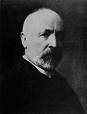
\includegraphics[width=0.3\textwidth]{image/Cantor.jpg}
\\
\centering{康托尔}
\end{figure}

康托尔(1845--1918)德国数学家, 集合论的创始人. 生于俄国圣彼得堡(今俄罗斯列宁格勒), 父亲是犹太血统的丹麦商人, 母亲出身艺术世家. 1856~年全家迁居德国的法兰克福,  先在一所中学, 后在威斯巴登的一所大学预科学校学习. 1862~年入苏黎世大学学工, 翌年转入柏林大学攻读数学和神学, 受教于库默尔、维尔斯特拉斯和克罗内克. 1866~年曾去格丁根学习一学期,  1867~年在库默尔指导下以解决一般整系数不定方程~$ax^2+by^2+cz^2=0$~求解问题的论文获博士学位. 毕业后受维尔斯特拉斯的直接影响, 由数论转向严格的分析理论的研究, 不久崭露头角. 他在哈雷大学任教(1869$\sim$1913年)的初期证明了复合变量函数三角级数展开的唯一性, 继而用有理数列极限定义无理数. 1872~年成为该校副教授, 1879~年任教授. 由于学术观点上受到的沉重打击, 使康托尔曾一度患精神分裂症,  虽在~1887~年恢复了健康, 继续工作, 但晚年一直病魔缠身. 1918~年~1~月~6~日在德国哈雷--维滕贝格大学
附属精神病院去世.

康托尔爱好广泛, 极有个性, 终身信奉宗教. 早期在数学方面的兴趣是数论, 1870~年他开始研究三角级数并由此产生~19~世纪末到~20~世纪初最伟大的数学成就\raisebox{0.5mm}{-----}集合论和超穷数理论的建立. 除此之外,  他还努力探讨在新理论创立过程中所涉及的数理哲学问题.

康托尔对数学的主要贡献是集合论和超穷数理论. 由康托尔首创的全新且具有划时代意义的集合论, 是自古希腊时代的两千多年以来, 人类认识史上第一次给无穷建立起抽象的形式符号系统和确定的运算, 它从本质上揭示了无穷的特性, 使无穷的概念发生了一次革命性的变化, 并渗透到所有的数学分支, 从根本上改造了数学的结构, 促进了数学的其他许多新的分支的建立和发展, 成为实变函数论、代数拓扑、群论和泛函分析等理论的基础, 还给逻辑和哲学带来了深远的影响.

不过康托尔的集合论并不是完美无缺的, 一方面, 康托尔对``连续统假设''和``良序性定理''始终束手无策; 另一方面, 19~和~20~世纪之交发现的布拉利--福蒂悖论、康托尔悖论和罗素悖论, 使人们对集合论的可靠性产生了严重的怀疑. 加之集合论的出现确实冲击了传统的观念, 颠覆了许多前人的想法, 很难为当时的数学家所接受, 遭到了许多人的反对, 其中反对的最激烈的是柏林学派的代表人物之一、构造主义者克罗内克. 克罗内克认为, 数学的对象必须是可构造出来的, 不可用有限步骤构造出来的都是可疑的, 不应作为数学的对象, 他反对无理数和连续函数的理论, 同样严厉批评和恶毒攻击康托尔的无穷集合和超限数理论不是数学而是神秘主义. 他说康托尔的集合论空空洞洞毫无内容,  除了克罗内克之外, 还有一些著名数学家也对集合论发表了反对意见. 法国数学家庞加莱说:``我个人, 而且还不只我一人, 认为重要之点在于, 切勿引进一些不能用有限个文字去完全定义好
的东西''. 他把集合论当作一个有趣的``病理学的情形''来谈, 并且预测说:``后一代将把集合论当作一种疾病
而人们已经从中恢复过来了''. 德国数学家魏尔斯特拉斯认为, 康托尔关于基数的等级观点是``雾上之雾''. 克莱因也不赞成集合论的思想. 数学家施瓦兹原来是康托尔的好友, 但他由于反对集合论而同康托尔断交. 集合论的悖论出现之后, 他们开始认为集合论根本是一种病态, 他们以不同的方式发展为经验主义、
半经验主义、直觉主义、构造主义等学派, 在基础大战中, 构成反康托尔的阵营.
1884~年, 由于连续统假设长期得不到证明, 再加上与克罗内克的尖锐对立, 精神上屡遭打击, 5~月底, 他支持不住了, 第一次精神崩溃. 他的精神沮丧, 不能很好地集中研究集合论, 从此深深地卷入神学、哲学及文学的争论而不能自拔. 不过每当他恢复常态时, 他的思想总变得超乎寻常的清晰, 继续他的集合论的工作.

康托尔的集合论得到公开的承认和热情的称赞应该说首先在瑞士苏黎世召开的第一届国际数学家大会上表现出来. 瑞士苏黎世理工大学教授胡尔维茨在他的综合报告中, 明确地阐述康托尔集合论对函数论的进展所起的巨大推动作用, 这破天荒地向国际数学界显示出了康托尔的集合论
不是可有可无的哲学, 而是真正对数学发展起作用的理论工具. 在分组会上, 法国数学家阿达玛也报告康托尔对他的工作的重要作用. 随着时间的推移, 人们逐渐认识到集合论的重要性. 希尔伯特高度赞誉康托尔的集合论是``数学天才最优秀的作品'', ``人类纯粹智力活动的最高成就之一'', ``这个时代所能夸耀的最巨大的工作''. 在~1900~年第二届国际数学家大会上, 希尔伯特高度评价了康托尔工作的重要性, 并把康托尔的连续统假设
列入~20~世纪初有待解决的~23~个重要数学问题之首. 当康托尔的朴素集合论出现一系列悖论时, 克罗内克的后继者布劳威尔等人借此大做文章, 希尔伯特用坚定的语言向他的同代人宣布:``没有任何人能将我们从康托尔所创造的伊甸园中驱赶出来''.
\bigskip

\section*{(二) 勒贝格}

\begin{figure}[!h]
\centering
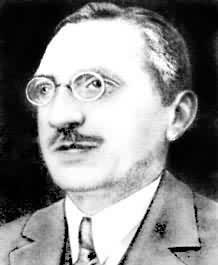
\includegraphics[width=0.3\textwidth]{image/Lebesguetu.jpg}
\\
\centering{勒贝格}
\end{figure}

勒贝格(1875--1941)法国数学家, 生于法国博韦, 父亲是一名印刷厂职工, 酷爱读书, 很有教养. 在父亲的影响下, 勒贝格从小勤奋好学, 成绩优秀, 特别擅长计算. 不幸, 父亲去世过早, 家境衰落. 在学校老师的帮助下进入中学, 后又转学巴黎. 1894~年考入高等师范学校.

1897~年大学毕业后, 勒贝格在该校图书馆工作了两年. 在这期间, 出版了波雷尔关于点集测度的新方法的《函数论讲义》, 特别是研究生贝尔发表了关于不连续实变函数理论的
第一篇论文. 这些成功的研究工作说明在这些崭新的领域中进行开拓将会获得何等重要的成就, 从而激发了勒贝格的热情. 从~1899$\sim$1902~年勒贝格在南锡的一所中学任教, 虽然工作繁忙, 但仍孜孜不倦地研究实变函数理论, 并于~1902~年发表了博士论文``积分、长度、面积'', 在这篇文章中, 勒贝格创立了后来以他的名字命名的积分理论. 此后, 他开始在大学任教(1902$\sim$1906~年在雷恩;1906$\sim$1910~年在普瓦蒂埃), 并出版了一些重要著作:
《积分法和原函数分析的讲义》(1904~年)、《三角级数讲义》(1906~年), 接着, 勒贝格又于~1910$\sim$1919~年在巴黎大学担任讲师, 1920~年转聘为教授, 这时他又陆续发表了许多关于函数的微分、积分理论的研究成果. 勒贝格于~1921~年获得``法兰西学院教授''称号, 翌年作为约当的后继人被选为巴黎科学院院士.

勒贝格对数学的主要贡献属于积分论领域, 这是实变函数理论的中心课题. 19~世纪以来, 微积分开始进入严密化的阶段. 1854~年, 黎曼引入以他的名字命名的积分, 这一理论的应用范围主要是连续函数. 随着维尔斯特拉斯和康托尔工作的问世, 在数学中出现许多``奇怪''的函数与现象, 致使黎曼积分理论暴露出较大的局限性. 几乎与
这一理论发展的同时(1870$\sim$1880~年), 人们就已广泛地开展了对积分理论的改造工作. 当时, 关于积分论的工作主要集中在
无穷集合的性质的探讨, 而无处稠密的集合具有正的外``容度''性质的发现, 使集合的测度概念在积分论的研究中占有重要地位. 积分的几何意义是曲线围成的面积, 黎曼积分的定义是建立在对区间长度的分割的基础上的. 因此, 人们自然会考虑到如何把长度、
面积等概念扩充到更广泛的集合类上, 从而把积分概念置于集合测度理论的框架之中. 这一思想的重要性在于使人们认识到:
集合的测度与可测性的推广将意味着函数的积分与可积性的推广. 勒贝格积分正是建立在勒贝格测度理论的基础上的, 它是黎曼积分的扩充.

为勒贝格积分理论的创立做出重要贡献的首先应推约当, 他在《分析教程》一书中阐述了后人称谓的约当测度论, 并讨论了定义在有界约当可测集上的函数, 采用把区域分割为有限个约当可测集的办法来定义积分. 虽然约当的测度论存在着严重的缺陷(例如存在着不可测的开集, 有理数集不可测等), 而且积分理论也并没有做出
实质性的推广, 但这一工作极大地影响着勒贝格研究的视野. 在这一方向上迈出第二步的杰出人物是波雷尔, 1898~年在他的《函数论讲义》中向人们展示了``波雷尔集''的理论. 他从~$\R$~中的开集是构成区间的
长度总和出发, 允许对可列个开集作并与补的运算, 构成了所谓以波雷尔可测集为元素的~$\sigma$-代数类, 并在其上定义了测度. 这一成果的要点是使测度具备完全可加性(约当测度只具备有限可加性), 即对一列互不相交
的波雷尔集~$\{E_n\}$, 若其并集是有界的, 则其并集的测度等于每个~$E_n$~的测度的和. 此外, 他还指出:集合的测度和可测性是两个不同的概念. 但在波雷尔的测度思想中, 却存在着不是波雷尔集的约当可测集(这一点很可能是使他没有进一步开创积分理论的原因之一). 特别是其中存在着零测度的稠密集, 引起了一些数学家的反感. 然而勒贝格却洞察了这一思想的深刻意义并接受了它. 他突破了约当对集合测度的定义中所作的有限覆盖的限制, 以更加一般的形式发展和完善了波雷尔的测度观念, 给出了集合测度的分析定义:

设~$E \subset [a,\,b]$, 考虑可数多个区间~$\{I_i\}$~对~$E$~作覆盖. 定义数值
\[
m^*(E)=\inf\Big\{ \mathop{\textstyle{\sum}}_i \big| I_i \big|: \: \medcup_i I_i \supset E \Big\}
\]
为勒贝格外测度, 且若
\[
m^*(E) + m^*\big( [a,\,b]-E \big) = b-a
\]
则称~$E$~为可测集(即~$E$~是勒贝格可测的).

在此基础上, 勒贝格引入了新的积分定义:

对于一个定义在~$[a,\,b]$~上的有界实值函数~$f(x)~(M_1 \leqslant f(x) \leqslant M_2)$, 作~$[M_1,\,M_2]$~的分割~$\delta$
\[
M_1 = y_0 < y_1 < \cdots < y_{n-1} < y_n = M_2
\]
令
\[
E_i = \big\{x \in [a,\,b]: \: y_{i-1} \leqslant f(x) \leqslant y_i \big\}, \quad i=1,\,\cdots,\,n
\]
并假定这些集合是可测的(即~$f(x)$~是勒贝格可测函数), 并用~$m(E_i)$~表示~$E_i$~的
勒贝格测度. 考虑和式
\[
s_\delta = \sum_{i=1}^n y_{i-1} \cdot m(E_i), \quad S_\delta = \sum_{i=1}^n y_i \cdot m(E_i)
\]
如果当~$\max\{y_i - y_{i-1}\} \to 0$~时, $s_\delta$~与~$S_\delta$~趋于同一极限值, 则称此值为~$f(x)$~在~$[a,\,b]$~上的积分.

勒贝格曾对他的这一积分思想做过一个生动有趣的描述:

\begin{quote}
``我必须偿还一笔钱. 如果我从口袋中随意地摸出来各种不同面值的钞票, 逐一地还给债主直到全部还清, 这就是黎曼积分;不过, 我还有另一种做法, 就是把钱全部拿出来并把相同面值的钞票放在一起, 然后再一起付给应还的数目, 这就是我的积分.''
\end{quote}


从他的这一新思想中, 任何约当可测集、波雷尔可测集都是勒贝格可测集. 勒贝格积分的范围包括了由贝尔引入的一切不连续函数.

从数学发展的历史角度看, 新的积分理论的建立是水到渠成的事情. 但是可贵的是, 与同时代的一些数学家不同, 在勒贝格看来, 积分定义的推广只是他对积分理论研究的出发点, 他深刻的认识到, 在这一理论中蕴含着一种新的
分析工具, 使人们能在相当大范围内克服黎曼积分中产生的许多理论困难. 而这些困难所引起的问题正是促使
勒贝格获得这一巨大成就的动力.

这方面的第一个问题是早在~19~世纪初期由傅里叶在关于三角级数的工作中不自觉地引发的: 当一个有界函数可以表示为一个三角级数时, 该级数是它的
傅里叶级数吗？这一问题与一个无穷级数是否可以逐项积分有着密切的关系. 傅里叶当时曾认为在其和为有界函数时
这一运算是正确的, 从而给上述问题以肯定的回答. 然而到了~19~世纪末期, 人们认识到逐项积分并不总是可行的, 甚至对于黎曼可积函数的一致有界的级数也是这样, 因为由该级数所表示的函数不一定是黎曼可积的. 这个问题的讨论
促使勒贝格在新的积分理论中获得了一个十分重要的结果\raisebox{0.5mm}{-----}控制收敛定理. 作为一个特殊情形他指出, 勒贝格可积的
一致有界级数都可以逐项进行积分, 从而支持了傅里叶的结论. 逐项积分在本质上就是积分号下取极限的问题, 它是积分论中经常遇到的最重要的运算之一. 从而这一定理的创立显示出勒贝格积分理论的极大优越性.

微积分基本公式
\[
\int_a^x f'(x) \mathrm{d} x = f(x)-f(a), \quad x \in [a,\,b]
\]
是微积分学的核心. 然而这一公式的运用在黎曼积分意义下却有较大的局限性. 在~1878$\sim$1881~年间, 迪尼和沃尔泰拉曾构造了这样的函数, 它们具有有界的导函数, 但是导函数不是黎曼可积的, 从而基本定理
对此是不适用的. 此后, 联系到黎曼积分对无界函数的推广也发现了类似的困难. 然而, 在新的积分理论中, 勒贝格指出, 对有界函数来说, 这一困难是不存在的. 在~$f'(x)$~是有限值但无界的情形, 只要是可积的, 基本定理仍是成立的, 而且这正相当于~$f(x)$~是有界变差函数. 同时, 逆向问题也被人们提出来了:
何时一个连续函数是某个函数的积分？为此, 哈纳克曾导入了后来叫作绝对连续的函数. 约在~1890~年期间, 绝对连续函数就被当作绝对收敛的积分
的特征性质来研究, 虽然还没有人能真正证明任何绝对连续函数都是一个积分. 然而, 勒贝格通过对于导数
几乎处处为零但函数本身并非常数的函数的考察, 认识到在他的积分意义下, 上述结论是正确的. 从而得出了积分与原函数之间的一个完整结果: 微积分基本公式成立的充要条件是, $f(x)$~是~$[a,\,b]$~
上的绝对连续函数.

另一个与积分论有关的问题是曲线的长度问题. 19~世纪前期, 很少有人注意到一条曲线长度的定义和可求长问题. 一般都认为以~$y=f(x)~(a \leqslant x \leqslant b)$~所描述的曲线段总是有长度的, 且长度可用
\[
L=\int_a^b \big[ 1+[f'(x)]^2 \big]^\frac{1}{2} \mathrm{d} x
\]
表示. 杜布瓦雷蒙在研究关于两点间长度最短的曲线的变分问题时, 从狄利克雷关于函数的一般观点出发探讨了曲线长度的概念. 由于用到了极限过程这一分析手段, 他认为积分理论对曲线长度的概念和可求长性质的陈述是必不可少的. 而到了~19~世纪末期, 这一见解由于希弗尔举出了反例而更为尖锐, 这一反例致使定积分
\[
\int_{x_0}^{x_1} \big[ 1+[f'(x)]^2 \big]^\frac{1}{2} \mathrm{d} x
\]
在黎曼积分的定义下没有意义. 勒贝格对这一问题很感兴趣, 并应用他的积分理论中的方法和结果, 证明了曲线长度与积分概念是密切相关的, 从而恢复了杜布瓦雷蒙断言的可信性.

勒贝格关于微积分基本公式和曲线可求长理论的研究, 促使他发现有界变差函数是几乎处处可微的这一事实.
%\footnote{约当曾指出不定积分是有界变差函数. }% 
这一定理的重要性在于: 人们对连续函数的可微性已经讨论
了一个多世纪, 在~19~世纪的几乎前半个世纪, 人们还一直认为连续函数在其定义区域中绝大多数点上都是
可微的. 虽然连续函数总被误认为是逐段单调的, 但这使单调性与可微性联系起来了, 尽管是脆弱的. 到~19~世纪末期, 这一看法逐渐被人怀疑, 甚至有些其地位不低于维尔斯特拉斯的数学家都觉得存在这无处可微的连续的单调函数. 于是, 在这一意义下, 勒贝格的定理支持了老一代数学家的直觉印象.

在传统的关于二重积分与累次积分的恒等性定理上, 黎曼积分也反映出它的不足之处, 人们发现了使该定理不成立的
例子. 而作为一个结论, 这一定理的传统说法必须修改, 然而在把积分推广到无界函数的情形时, 这一修改变得更加严峻. 对此, 勒贝格的重积分理论, 使得用累次积分来计算二重积分的函数范围扩大了. 他在~1902~年给出的一个结果奠定了~1907~年富比尼创立的著名定理的基础.

\setcounter{footnote}{0}

勒贝格积分理论作为分析学中的一个有效工具的出现, 尤其是他在三角级数中应用的高度成功, 吸引了许多数学家的兴趣. 例如法都、里斯、费舍尔等都来探讨有关的问题, 使这一领域开始迅速发展, 其中特别是里斯关于~$L^p$~空间的工作\footnote{勒贝格可积函数的全体
构成的距离空间是完备的. }, 使得勒贝格积分在积分方程和函数空间的理论中持久地占有重要的位置.

虽然勒贝格在最初阶段专注于他自己的积分理论, 然而在激励抽象测度和积分论研究的开展上, 他的工作仍是先导性的. 1910~年, 勒贝格发表题为~``关于不连续函数的积分''的重要专题报告. 在这里他不仅把积分、微分理论推广到~$n$~维空间, 而且引入了可数可加集合函数的概念(定义在勒贝格可测集类上), 指出这些函数是定义在集合类上的有界变差函数. 正是因为对于
有界变差与可加性概念之间联系的考察, 使得拉东作出了更广的积分定义, 其中把斯蒂尔杰斯积分和勒贝格积分作为它的特殊情形. 他还在~1913~年的文章中指出, 勒贝格的思想在更一般的背景上也是有效的.

勒贝格的一生都献给了数学事业. 1922~年被推举为院士时, 他的著作和论文已达~90~多种之多, 内容除积分理论外, 还涉及集合与函数的构造\footnote{后来由苏联数学家卢津及其他学者进一步做出发展. }、变分法、曲面面积以及维数理论等重要课题. 在勒贝格生前最后~20~年, 研究工作仍然十分活跃并反映出广泛的兴趣, 不过作品内容大都涉及教育、历史等.

勒贝格的工作是对本世纪科学领域的一个重大贡献, 但和科学史上所有新思想运动一样, 并不是没有遇到阻力的. 原因是在勒贝格的研究中扮演了重要角色的那些不连续函数和不可微函数被人认为违反了所谓的完美性法则, 是数学中的变态和不健康部分. 因此, 他的工作受到了某些数学家的漠视, 甚至有人曾企图阻止他关于一篇讨论不可微曲面的论文的发表. 勒贝格曾感叹地说:``我被称为是一个没有导数的函数的那种人了！''
然而, 不论人们的主观愿望如何, 这些具有种种奇异性质的对象都自动地进入了研究者曾企图避开它们的问题之中. 勒贝格充满信心地指出:``使得自己在这种研究中变得迟钝了的那些人, 是在浪费他们的时间, 而不是在从事有用的工作. ''

由于在实变函数理论方面的杰出成就, 勒贝格相继获得胡勒维格奖(1912~年);
彭赛列奖(1914~年)和赛恩吐奖(1917~年). 许多国家和地区(如伦敦、罗马、丹麦、
比利时、罗马尼亚和波兰)的科学院都聘他为院士, 许多大学授予他名誉学位, 以表彰他的贡献.

\bigskip

\section*{(三) 黎曼}

\begin{figure}[!h]
\centering
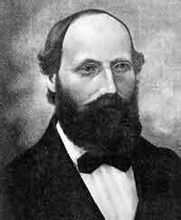
\includegraphics[width=0.3\textwidth]{image/Riemanntu.jpg}
\\
\centering{黎曼}
\end{figure}

1826~年~9月~17~日, 在德国汉诺威的布列斯伦茨, 黎曼(1826--1866)出生在一个乡下牧师之家, 是六个孩子中的次子. 黎曼从小酷爱数学. 他~6~岁时开始学习算术, 并显现出他的数学天才. 他不仅能解决所有留给他的数学问题, 而且还经常提一些问题来捉弄他的兄弟姐妹. 10~岁时他跟一位职业教师学习高级算数和几何, 很快便超过了老师, 常常对一些问题能做出更好的答案.

黎曼~14~岁时到汉诺威市上中学. 由于经济拮据, 他总是靠步行奔波于汉诺威市与乡间小村庄之间. 当然他更没钱去买参考书. 幸运的是中学校长及时地发现了他的数学才能, 考虑到他经济上的困难, 校长特许黎曼可以从自己私人藏书室里借阅数学书籍. 在校长的
推荐下, 黎曼借了一部数学家勒让德的《数论》, 这是一部共~859~页的四大本的名著. 黎曼十分珍惜这种读书机会, 他如饥似渴地自学起来, 六天之后, 黎曼便学完并归还了这本书. 校长问他:``你读了多少？''黎曼说:``这是一本了不起的书, 我已经掌握了它. ''几个月之后, 校长就这本书的内容考他, 黎曼对答如流, 并且回答得很全面. 利用校长的藏书, 黎曼还抓紧时间很快地
自学了大数学家欧拉的著作, 由此掌握了微积分及其分支. 黎曼
不仅从欧拉的著作中学到了数学知识, 还学到了欧拉研究数学的技巧.

19~岁时, 黎曼进入格丁根大学学习, 为了在经济上帮助家庭以尽快找到一个有报酬的
工作, 他先攻读哲学和神学. 但是, 除了这两门课程以外, 他也去听数学、物理学课程. 他听了斯特恩关于方程论和定积分、高斯关于最小二乘法以及戈尔德斯米特关于地磁学的
数学讲座, 对数学专业产生了难以割舍的兴趣.

黎曼向父亲讲述了这一切, 请求允许自己改学数学专业. 父亲由衷地同意了他的请求. 黎曼极为高兴, 并深深地感激父亲. 1847~年, 为了师从更多的大师, 黎曼转学到柏林大学, 就学于大数学家雅可比、
狄利克雷、斯泰纳和艾森斯坦门下. 他从雅可比那里学到高等力学和高等代数, 从狄利克雷那
里学到数论和分析学, 从斯泰纳那里学到现代几何, 从艾森斯坦那里学到椭圆函数论. 在此期间, 他极为勤奋, 甚至放假期间也不休息. 1847~年秋假, 黎曼找到几份巴黎科
学院《院刊》, 上面载有数学家柯西新发表的关于单复变量解析函数的论文, 他一眼便看
出这是一种新数学理论, 于是一连几个星期闭门不出, 潜心研究柯西的论文, 并酝酿出他
在这个专题上的新见解, 为四年后撰写博士论文``单复变量函数的一般理论的基础''奠定了
基础.

黎曼不仅认真研读大师的学术专著, 而且虚心地向大师求教. 有一次, 狄利克雷来格
丁根度假, 黎曼趁此机会向他求教数学问题, 并将自己未定稿论文交给他, 请他提意见. 狄利克雷被黎曼的谦虚、真诚和天才迷住了. 他与黎曼长谈了两个小时, 给黎曼的论文提
了不少意见, 给黎曼正在研究的课题作了许多指点, 黎曼深感受益匪浅, 他说没有狄利克
雷的指点, 他将不得不在图书馆里做好几天的吃力研究. 生活虽然清贫, 但学习极为勤勉, 这使得黎曼在大学毕业时获得了丰硕的成果. 1851~年底, 黎曼将其博士论文呈交给大数学家高斯审阅. 高斯在看了论文之后兴奋不已, 对黎曼的论文做出了高度评价, 这对高斯来说是罕见的. 高斯评语道:``黎曼先生交来的论文提供了令人信服的证据, 说明作者对该文所论述的这一问题做了
全面深入的研究, 说明作者具有创造性的、活跃的、真正的数学头脑, 具有灿烂丰富的创造力. ''

1852~年初, 黎曼凭借优异的学术表现取得了博士学位, 并留在了格丁根大学. 19~世
纪中叶的德国, 科学几乎与国家的经济全然无关. 大学的设立仅在训练律师、医师、教师
和传教士, 以及提供贵族子弟和富家子弟度过引人侧目及受尊敬的岁月的场所. 只有正
教授才可以领政府的津贴, 并且可以教正规标准课程, 这些课程都是一些基础科目.上课
的学生多, 因此教授收到的学费也就多了, 这就是为什么当时课程水准低落的原因, 因为
如果课程太难, 就没有办法收到许多学生, 从而影响到教授们的收入, 毕竟贵族子弟和富
家子弟上大学的目的并非真心向学. 讲师们则没有政府津贴并且轮不到教基本正规课程的
机会, 全然靠来听课的学生的学费维生, 通常, 听课的学生不会多, 因此收入也就相当微
薄, 生活非常困苦. 担任讲师是成为正教授的必经途径, 但是却没有明文规定什么时候能
将一位讲师升级为教授, 为了照顾特別值得重视的学者而却没有正教授的空缺时, 政府可
任命他为``客座教授'', 使他具有教基本正规课程的资格, 增多他的收入, 但是这个任命
附有条件, 言明政府不付任何津贴. 因此, 在担任讲师期间, 黎曼没有任何自主的生活费
来源, 生活依旧贫穷. 但黎曼不顾生活上的贫困, 仍然把全部精力投向数学. 他认为只要
能够勉强维持生活, 能够让他研究数学, 他就心满意足了. 他从不因经济上的拮据而感到沮丧. 他一方面积极准备``无薪讲师''的就职演讲论文, 另一方面认真从事数学物理方面的研究工作. 他的
就职论文具有相当的难度. 当初为了确定论文的选题, 他向高斯提交了~3~个题目, 以便让高
斯在其中选定一个. 其中第~3~个题目是涉及几何基础的, 这个题目黎曼当时并没有多少案头
准备工作, 因此黎曼从心底里希望高斯不要选中它. 可是, 高斯对第~3~个题目却深有研究, 他已思考这个问题达~60~年之久. 出于想看看黎曼对这个深奥的问题会做些什么样的创造性
工作, 高斯指定第~3~个题目作为黎曼就职演讲论文的题目. 事后, 黎曼在向父亲谈起这件事
时说, ``所以我又处在绝境中了'', ``我不得不做出这个题目''.

对数学物理研究, 黎曼也具有无限的热情, 他当时曾对人说:``我对于把一切与物理
规律结合起来的数学研究非常入迷. ''``我通过对电、光、磁等之间联系的总研究, 发现
了对这个现象的解释. 这件事对我很重要, 因为这是我第一次能够把我的工作应用到未知
的现象上. ''这两项研究在当时都是高水平的, 因而也是极困难的. 黎曼不顾生活清贫、
营养不良, 超负荷地忘我工作, 长时期过度紧张地思索, 以致他常常体力衰竭, 甚至
病倒. 一旦身体稍有复原, 他又继续研究. 功夫不负有心人, 1854~年~6~月~10~日, 黎曼以``关
于构成几何基础的假设''论文做了就职演讲, 受到了与会数学家们的认可和好评. 高斯听
完之后大为惊异, 感到这个年轻人处理这个难题非常之好, 他赞不绝口. 黎曼的这篇论文
被人们认为是~19~世纪数学史上的杰作之一.

1855~年格丁根大学开始给黎曼发薪金, 但相当的低, 一年仅相当于~200~美元. 这一年黎
曼~29~岁, 他家里遭到巨大的不幸, 父亲和一个妹妹相继去世, 原来依靠父亲生活的~3~个妹妹
失去了生活来源. 于是黎曼和他的哥哥两人挑起了照顾~3~个妹妹生活的担子, 黎曼时时为一
家人的生活感到焦虑. 1857~年黎曼一年的薪金被加到相当于~300~美元的水平. 由于收入不多, 又要照顾~3~个妹妹, 生活担子重, 黎曼连自己的婚姻大事都不敢考虑. 然而就在这一年, 不幸又从天而降, 黎曼的哥哥又去世了, 这对黎曼来说如同雪上加霜, 照料~3~个妹妹生活的
担子全部落在他一人的肩上. 从~1855~年到~1859~年这~5~年中, 经济拮据、生活清贫一直困绕着
黎曼, 有时一家甚至陷入对口粮都需要算计的地步. 就是在这种情况下, 黎曼仍不顾物质
生活的贫乏, 全身心地投入到数学研究工作之中, 在科学的崎岖小道上艰苦奋斗, 并获得
了令人惊异的成就. 他在数学上的许多重要成果都是在这个时期内完成的. 他对阿贝尔积
分和阿贝尔函数的研究, 开创了现代代数几何;他首创用复解析函数研究数论问题, 开创
了现代意义的解析数论;他对超几何级数的研究, 推动了数学物理和微分方程理论的发展. 随着研究成果的问世, 黎曼在数学界的学术声望迅速提高. 他受到许多世界著名数学家
的赞扬, 获得了一个科学家通常可能得到的最高荣誉.

1859~年黎曼~33~岁时, 高斯去世, 他被任命为格丁根大学正教授, 成为继狄利克雷之后
高斯的第二个继任者. 这时黎曼的生活才开始得到改善, 才开始考虑个人的婚姻问题, 并
在~36~岁时与朋友的妹妹结了婚, 一年后, 他的女儿出生在比萨. 但是, 长时期清贫的生活、
过度的操劳、发奋的研究, 使得黎曼身体虚弱、精力衰竭. 1862~年黎曼患了胸膜炎, 不久又患了肺病, 
一年后又患了黄疽病. 在病魔缠身之际, 只
要有一些力气, 黎曼仍坚持数学研究工作. 虽然这个时期黎曼积极就医和疗养, 但因病入
膏盲终无疗效, 1866~年~7~月~20~日, 黎曼那颗纯洁、高尚的心停止了跳动, 他过早地离开了人
世, 也过早地离开了数学, 终年仅~40~岁.

黎曼是数学史上最具独创性精神的数学家之一, 他在众多的数学领域里做出了许多奠
基性和创造性的研究工作\raisebox{0.5mm}{-----}他从几何方向开创了复变函数论;是现代意义的解析数论的奠
基者;他亲手建立了黎曼几何, 是组合拓扑学的开拓者;他对微积分的严格处理作出了重
要贡献;在数学物理和微分方程等领域内也成果丰硕. 1859~年, 黎曼被选为柏林科学院通
讯院士, 1866~年他被选为法国巴黎科学院通讯院士和英国皇家学会国外会员.

%%%%%%%%%%%%%%%%%%%%%%%%%%%%%%%%%%%%%Fubini%%%%%%%%%%%%%%%%%%%%%%%%%%%%%%%%%%%%%%%%%
%\bigskip
%
%\section*{4. 富比尼(Fubini)}
%
%\begin{figure}[!h]
%\centering
%
\includegraphics[width=0.3\textwidth]{images/Fubini.jpg}
%\caption{富比尼(Fubini)}
%\end{figure}
%
%富比尼(G. Fubini, 1879-1943)意大利数学家, 最著名是他的富比尼定理. 富比尼生于威尼斯,
% 早年即因他的老师们和他作数学老师的父亲影响而醉心数学. %1896~年他进了~Scuola Normale Superiore di Pisa, 跟随著名数学家乌利塞·迪尼和路易吉·比安基学习. 他早时已经名声鹊起, 1900~年发表的博士论文《椭圆空间中的克利福德平行》, %在比安基广泛流传的微分几何著作中作了讨论. %
%他获得博士后, 开始担任一连串的教授职位. 1901~年他在西西里的卡塔尼亚大学开始教学, 不久后转到热那亚大学; 1908~年转到都灵的~Politecnico, 接着在都灵大学, 他留在这里数十年. %他这时的研究主要在数学分析, 特别是微分方程、泛函分析和复分析; 但他也研究了变分学、群论、非欧几里得几何和射影几何等学科. %第一次世界大战开始, 他转为从事应用层面的工作, 研究发射炮弹的准确度; 战后他的研究依然朝向应用, 工作成果应用到电路和声学问题. 1939~年, 富比尼年已六旬, 将近退休时, 贝尼托·墨索里尼的法西斯党采取阿道夫·希特勒的纳粹党鼓吹了数年的
%反犹太政策. 身为犹太人, 富比尼担心家庭的安全, 所以应邀到普林斯顿大学任教, 4~年后于纽约市逝世.
\nocite{*}
\printbibliography
\addcontentsline{toc}{chapter}{参考文献}

\end{document}

% 运行方式Tinytex + RStudio
% library(tinytex)
% xelatex("main.tex", bib_engine = "biber")
